% This is LLNCS.DEM the demonstration file of
% the LaTeX macro package from Springer-Verlag
% for Lecture Notes in Computer Science,
% version 2.4 for LaTeX2e as of 16. April 2010
%

%\iffalse

\documentclass[12pt,final]{llncs}
\usepackage{iftex}
\usepackage{calc}
\usepackage{lastpage}

%\fi % above for final

%\documentclass[12pt]{llncs}
%\usepackage{todonotes}
%\usepackage{nla}

\ifPDFTeX
\usepackage{amsmath,amssymb}
\usepackage[T2A]{fontenc}
\usepackage[utf8]{inputenc}
\usepackage[english,russian]{babel}
\fi
\usepackage{amscd}
\usepackage{amsfonts,amsmath,array}
\usepackage{amssymb}
%\usepackage[dvips]{graphicx}
\usepackage{graphicx}
\usepackage{longtable,cite,wrapfig}
% \usepackage{makeidx}


 \usepackage[russian]{nla}
 \usepackage{bm}
 \usepackage{euscript}
 \usepackage{upgreek}
 \usepackage{fancyhdr}
 \usepackage{lastpage}

 \usepackage{enumitem}
 \usepackage{pifont}

 \setlist[itemize]{label=\ding{113}}

%\usepackage{showframe}
%
%\usepackage{makeidx}  % allows for indexgeneration
%
\usepackage{fancyhdr}
\pagestyle{fancy}
\lhead{}
\chead{}
\rhead{}
\lfoot{}
\cfoot{\normalsize{\textrm{\thepage}}}
\rfoot{}
\renewcommand{\headrulewidth}{0pt}
\renewcommand{\footrulewidth}{0pt}
\pagestyle{fancy}
% \usepackage{etoolbox} % for "\patchcmd" macro
% \makeatletter
% \patchcmd{\ps@headings}{\rlap{\thepage}}{}{}{}
% \patchcmd{\ps@headings}{\llap{\thepage}}{}{}{}
% \makeatother
% \pagestyle{headings}

\RequirePackage{algorithm}
\RequirePackage{algpseudocode}

%%%%%%%%%%%%%%%%%%%%%%%%%%%%%%%%%%%%%% below from files 2022
\newcommand{\rd}{\mathbb{R}^d}
\newcommand{\prd}{\mathcal{P}^p(\rd)}
\newcommand{\pp}{\mathbb{P}}
\usepackage{amssymb}



% Delova-r-f:
\usepackage{bm}
\def\dfrac#1#2{\displaystyle{#1\over #2}}
%\def\Div{\mbox{div}\,}
%\def\bB{{\bf B}}
\def\bx{{\bf x}}
%\def\bE{{\bf E}}
\def\bV{{\bf V}}
\def\bv{{\bf v}}
\def\br{{\bf r}}
\def\bp{{\bf p}}
%\def\bV{{\bf V}}


%Lade:
%\usepackage{amsmath}
\newcommand{\Si}[1][\theta]{\sin_{\Omega}{#1}}

\newcommand{\So}[1][\theta^o]{\sin_{\Omega^o}{#1}}

\newcommand{\Ci}[1][\theta]{\cos_{\Omega}{#1}}

\newcommand{\Co}[1][\theta^o]{\cos_{\Omega^o}{#1}}

\newcommand{\Ti}[1][\theta]{\tan_{\Omega}{#1}}

\newcommand{\To}[1][\theta^o]{\tan_{\Omega^o}{#1}}

\newcommand{\ATi}{\arctan_{\Omega}\theta}

\newcommand{\ATo}[1][\theta^o]{\arctan_{\Omega^o}{#1}}


%Yufereva:






%%%%%%%%%%%%%%%%%%%%%%%%%%%%%%%%%%%% above from files 2022


\begin{document}%
%
\frontmatter          % for the preliminaries
\setcounter{page}{1}
%
%\pagestyle{headings}  % switches on printing of running heads
%\addtocmark{~} % additional mark in the TOC
%

\begin{center}
{\bf
  \thispagestyle{empty}
  \pagestyle{fancy}

   	Matrosov Institute for System Dynamics and Control Theory of  SB RAS\\[0.3em]

 	Sobolev Institute of Mathematics  of SB RAS\\[0.3em]

  Krasovskii Institute of Mathematics and Mechanics of UrB RAS\\[0.3em]

 	Irkutsk State University\\[0.3em]
 	Mathematical center in Akademgorodok   }


%\vspace{2cm}
\vfill

{  \Large Proceedings of the 7th International Conference on\\[0.3em]

Nonlinear Analysis and Extremal Problems\\[0.3em]

  (NLA-2022)\\[0.2em] }

{\Large  Irkutsk, Russia, July 15--22, 2022 }

% \vspace{4cm}
\vfill
\vfill



Irkutsk\\
ISDCT SB RAS\\
2022

\end{center}

\newpage

\thispagestyle{empty}
\noindent{}UDC \ 517.9

 \vspace{3cm}

Proceedings of the 7th International Conference on Nonlinear
Analysis and Extremal Problems  (NLA-2022). Irkutsk\;:
ISDCT SB RAS, 2022, \pageref{LastPage}~p.\\
ISBN 978-5-6041814-2-3

 \vspace{1cm}

This volume contains proceedings of the 7th International Conference ``Nonlinear
Ana\-ly\-sis and Extremal Problems''  (NLA-2022). The conference talks present recent developments in
various fields of nonlinear analysis,  partial differential equations, dynamical systems,
calculus of variations, mathematical control theory, and optimization.

This volume is intended for researchers specializing in the corresponding fields of  ma\-the\-ma\-tics.

  \vspace{1cm}

NLA-2022  is a satellite of the International Congress of Mathematicians 2022 (ICM 2022)

 \vfill

  \vfill

 Scientific Editor: Prof. A.\;A. Tolstonogov\\[0.3em]

 Editors: E.\;Yu. Baturina, O.\;N. Samsonyuk\\[0.3em]

 Computer layout by E.\;A. Cherkashin

 \vfill



 \begin{flushright}
 \copyright ISDCT SB RAS, 2022
  \end{flushright}



\chapter*{Preface}
%




 \begin{englisharticle}

This volume contains proceedings of the 7th  International Conference ``Nonlinear Analysis and Extremal Problems'' (NLA-2022) that takes place in Irkutsk, Russia. NLA-2022 is a satellite of the International Congress of Mathematicians 2022 (ICM 2022) and is held on 15-22 July 2022. NLA-2022 aims at sharing recent advances in various areas of modern nonlinear analysis and exposing young researchers to some fast-paced topics in the field.

The main topics of the  conference are
\begin{itemize}
\item Nonlinear analysis and its applications,
\item Partial differential equations,
\item Dynamical systems,
\item Calculus of variations,
\item Mathematical control theory,
\item Optimization
\end{itemize}
The conference featured six lecture courses devoted to various aspects of theoretical and applied nonlinear analysis and control theory:
\begin{itemize}
\item \emph{``Geometry and topology of the spaces of measures''}\\ by  \textbf{Vladimir I. Bogachev} (Lomonosov Moscow State University, Russia),\smallskip
\item \emph{``Variational analysis and optimization theory: selected topics''}\\ by \textbf{Alexander Y. Kruger} (Federation University Australia, Australia),\smallskip
\item \emph{``Introduction to sub-Riemannian and sub-Finsler geometries from the optimal control viewpoint''}\\ by  \textbf{Lev V. Lokutsievskiy} (Steklov Mathematical Institute of RAS, Russia),
\item \emph{``Controllability and optimality''}\\ by \textbf{Georgii G. Magaril-Il'yaev} (Lomonosov Moscow State University, Russia),
\item \emph{``Optimal control of sweeping processes''}\\ by \textbf{Boris Sh. Mordukhovich} (Wayne State University, USA),
\item \emph{``Nonlinear Fokker-Planck-Kolmogorov equations''}\\ by \textbf{Stanislav V. Shaposhnikov} (Lomonosov Moscow State University, Russia).\smallskip
\end{itemize}








 \end{englisharticle}

%
\chapter*{Organization}
\vspace{-2em}
 \begin{englisharticle}
NLA-2022 is organized by Matrosov
Institute for System Dynamics and Control Theory of SB RAS in cooperation with
Sobolev Institute of Mathematics  of SB RAS,
  Krasovskii Institute of Mathematics and Mechanics of UB RAS,
 	Irkutsk State University, and Mathematical center in Akademgorodok (Novosibirsk).
 \end{englisharticle}


%
\vspace{-1em}
\section*{Program Commitee}
 \begin{englisharticle}

\textbf{Chairs:   }

\begin{tabular}{@{}p{6cm}@{}p{10cm}@{}}
  Alexander A. Tolstonogov &   Matrosov
Institute for System Dynamics and Control Theory of SB RAS (Russia)\\
Igor V. Bychkov &   Matrosov
Institute for System Dynamics and Control Theory of SB RAS (Russia)
\end{tabular}

\textbf{Committee members:}

\begin{tabular}{@{}p{5.5cm}@{}p{0.5cm}@{}p{10cm}@{}}
Vladimir I. Bogachev & & Lomonosov Moscow State University  (Russia)\\[0.5em]
Alexander G. Chentsov  &&  Krasovskii Institute of Mathematics and Mechanics of UrB RAS (Russia)\\[0.5em]
Gennadii V. Demidenko &&  Sobolev Institute of Mathematics of SB RAS (Russia)\\[0.5em]
Ivan A. Finogenko &&  Matrosov
Institute for System Dynamics and Control Theory of SB RAS (Russia)  (Russia)\\[0.5em]
Alexander L. Kazakov &&  Matrosov
Institute for System Dynamics and Control Theory of SB RAS (Russia) (Russia)\\[0.5em]
Yuri S. Ledyaev & & Western Michigan University  (USA)	\\[0.5em]
Nikolai Yu. Lukoyanov &&  Krasovskii Institute of Mathematics and Mechanics of UrB RAS (Russia)\\[0.5em]
Georgii G. Magaril-Il'yaev &&  Lomonosov Moscow State University  (Russia)\\[0.5em]
Manuel~D.P.~Monteiro   && University of Lisbon  (Portugal)\\ 
~~~~~~~~~ Marques && ~\\[0.5em]
Boris Sh. Mordukhovich &&  Wayne State University  (USA)\\[0.5em]
Alla A. Shcheglova &&  Matrosov
Institute for System Dynamics and Control Theory of SB RAS (Russia)\\[0.5em]
Vladimir N. Ushakov &&  Krasovskii Institute of Mathematics and Mechanics of UrB RAS (Russia)
 \end{tabular}









 \end{englisharticle}

\vspace{-1em}
%

%
\section*{Organizing Committee}

 \begin{englisharticle}
{\bf Chair:}   Vladimir A. Dykhta\\[0.5em]
%${}$\hspace{\parindent}
{\bf Secretary:}   Nikolay I. Pogodaev\\[0.5em]
${}$\hspace{\parindent}\textbf{Committee members:\\[0.5em]}
\begin{tabular}{@{${}$\hspace{\parindent}}p{5cm}@{}p{5cm}@{}p{5cm}@{}}
Anton S. Anikin&
  Elena V. Chistyakova &
  Alexey A. Kumachev\\
Anna A. Lempert &
Taras I. Madzhara &
Nadezhda S. Maltugueva \\
Pavel S. Petrenko &
Olga N. Samsonyuk&
Stepan P. Sorokin \\
Pavel S. Sorokovikov &
Maxim V. Staritsyn&
Tatiana S. Zarodnyuk
\end{tabular}




 \end{englisharticle}



 \begin{englisharticle}
  \tableofcontents
 \end{englisharticle}
\thispagestyle{fancy}
%
\mainmatter              % start of the contributions

%


\begin{englishtitle} % Настраивает LaTeX на использование английского языка
% Этот титульный лист верстается аналогично.
\title{Estimation Problem for Discrete Systems with Information Delays\thanks{Работа выполнена в рамках исследований, проводимых в Уральском математическом центре
при финансовой поддержке Министерства науки и высшего образования Российской Федерации
(номер соглашения \textnumero~075-02-2022-874).}}
% First author
\author{Boris Ananyev  \and Polina Yurovskikh 
}
\institute{IMM UB RAS, Yekaterinburg, Russia\\
  \email{abi@imm.uran.ru, polina2104@list.ru}}
% etc

\maketitle
\begin{abstract}
We consider an estimation problem for a linear stationary discrete system under
uncertainty with measurement delay. The problem is an approximation of the
corresponding problem for a continuous system. Restrictions on disturbances are
integral, on the initial state are geometric. The problem consists in constructing
information sets based on measurement data containing the true state of the system, and
is solved using cone programming methods. Convergence in the Hausdorff metric of the
set of the discrete problem to the corresponding set of the continuous system is
proved.
\keywords{discrete system, delay, guaranteed estimation, support function, conic optimization} % в конце списка точка не ставится
\end{abstract}
\end{englishtitle}

\iffalse


\documentclass[12pt]{llncs}
\usepackage[T2A]{fontenc}
\usepackage[utf8]{inputenc}
\usepackage[english,russian]{babel}
\usepackage[russian]{nla}
\usepackage[active]{srcltx}
\begin{document}
\fi

\title{Задача оценивания дискретных систем с запаздыванием в измерении
}
\author{Б.~И.~Ананьев   \and П.~А.~Юровских 
} % обязательное поле
\institute{ИММ УрО РАН, Екатеринбург, Россия\\
  \email{abi@imm.uran.ru, polina2104@list.ru}}
\maketitle
\begin{abstract}
Рассматривается задача оценивания для линейной стационарной дискретной системы в
условиях неопределенности с запаздыванием в измерении. Данная задача представляет собой
аппроксимацию соответствующей проблемы для непрерывной системы. Ограничения на
возмущения -- интегральные, на начальное состояние -- геометрические. Рассматриваемая
задача состоит в построении информационных множеств по данным измерения, содержащих
истинное состояние системы, и она решается с помощью методов конического
программирования. Доказывается сходимость в метрике Хаусдорфа множеств дискретной
задачи к соответствующему множеству непрерывной системы. \keywords{дискретная система,
запаздывание, гарантированное оценивание, опорная функция, коническая оптимизация}
\end{abstract}

Пусть задана дискретная система с наблюдением
\begin{equation}\label{Yurovskikh-eq1}
	\begin{gathered}
		x_k=Ax_{k-1} + bv_k, \ \ x_k\in\mathbb{R}^n, \ \ k\in1:N, \\
		y_k=Gx_{k-1} + cv_k + G_1x_{k-s},\ \ y_k\in\mathbb{R}^m,
	\end{gathered}	
\end{equation}
где $s\in \mathbb{N}$ --- задержка в получении наблюдений, $A,b,G,G_1$ --- матрицы
соответствующих размерностей. Неизвестные возмущения $v_k$ и начальное состояние $x_0$
подчинены ограничениям
\begin{equation}\label{Yurovskikh-eq2}
	\sum_{k=1}^N|v_k|^2\leq 1, \ \ x_0\in X_0,
\end{equation}
где $X_0 = \{x\in\mathbb{R}^n:|x_{(j)}-x_{(j)}^c| \leq \mu_{(j)}\}$ --- бокс,  $x_{(j)}^c
> 0 $,  $ \mu_{(j)} > 0$, $j = \{1,\ldots,n\}$.
\begin{definition}\label{Yurovskikh-Dfn2}
Семейство $\mathcal{X}^N(y)\subset\mathbb{R}^n$ назовем \emph{информационным множеством
(сокращенно ИМ)}, если оно состоит из всех векторов $x_N$, для каждого из которых
существует порождающая совместимая пара $(x_0,v_\bullet)$ при $1:N$, удовлетворяющая
ограничениям \eqref{Yurovskikh-eq2}.
\end{definition}

Из определения \ref{Yurovskikh-Dfn2} вытекает, что
$
	\mathcal{X}^N (y) = \{x_N \in \mathbb{R}^n | \min_v J^N(x_N,v_{1:N})\leq 1 - \sum_{k=1}^N |y_k|^2_C\},
$
где функционал представим в виде $J^N(x_N,v_{1:N}) = \sum_{k=1}^N |v_k|^2_{C_1} -|Gx_{k-1}|^2_C -
 |G_1x_{k-s}|^2_C - 2(cv_k)'CGx_{k-1} - 2(cv_k)'CG_1x_{k-s} - 2(G_1x_{k-s})'CGx_{k-1}  \leq p$. К виду функционала
можно прийти, используя ортогональное разложение $v_k=c'Ccv_k+C_1v_k$ в пространстве
$\mathbb{R}^q$, где $C_1=I_q-c'Cc$ --- ортогональная проекция на подпространство
ker$\,c$.

Поскольку замкнутое выпуклое множество однозначно определяется своей опорной функцией,
определим для  информационного множества системы \eqref{Yurovskikh-eq1} с ограничениями
\eqref{Yurovskikh-eq2} величину
\begin{equation}\label{Yurovskikh-eq5}
	\rho(l,\mathcal{X}^N(y)) = \max_{x_N} l'x_N, \ \ x_N \in \mathcal{X}^N(y), \ l  \in\mathbb{R}^{n}.
\end{equation}
При фиксированном $l$ значение опорной функции можно найти как решение задачи конического
программирования
\begin{equation}\label{Yurovskikh-eq7}
	\begin{gathered}
		||Q r|| \leq p, \ \
		Mr \leq w, \ \
		Hr = h,
	\end{gathered}
\end{equation}
где $r = (x_0, x_1, \dots, x_N, v_1,\dots,v_N )' \in \mathbb{R}^{n+(n+q)N}$. Суммарным
ограничениям \eqref{Yurovskikh-eq2} соответствует первое неравенство из
\eqref{Yurovskikh-eq7}, геометрическим ограничениям --- второе неравенство, а последнее
равенство описывает динамику системы  \eqref{Yurovskikh-eq1}.

В докладе приводится связь параметров непрерывной и дискретной задач и рассматриваются
примеры. Результаты работы продолжают исследования \cite{Yurovskikh-Ananyev} и используют
методы из \cite{Yurovskikh-Luenberger}.

\begin{thebibliography}{9} % или {99}, если ссылок больше десяти.
\bibitem{Yurovskikh-Ananyev} {   Ананьев~Б.И., Юровских~П.А.} О задаче оценивания с
    раздельными ограничениями на начальные состояния и возмущения~// Тр. Ин-та математики
    и механики УрО РАН. 2022. Т.~28, №~1. C.~27--39.

\bibitem{Yurovskikh-Luenberger} {  Luenberger~D.G, Ye~Y.} Conic Linear Programming. In:
    Linear and Nonlinear Prog\-ramming~// International Series in Operations Research and
    Management Science, 2016, vol 228. Springer, Cham.
    https://doi.org/10.1007/978-3-319-18842-3 6
\end{thebibliography}


%\end{document}


 \begin{englisharticle}



\iffalse
% !TeX spellcheck = en_US
%%%%%%%%%%%%%%%%%%%%%%%%%%%%%%%%%%%%%%%%%%%%%%%%%%%%%%%%%%%%%%%%%%%%%%%%
%
% This is the template file for the 6th International conference
% NONLINEAR ANALYSIS AND EXTREMAL PROBLEMS
% June 25-30, 2018
% Irkutsk, Russia
%
%%%%%%%%%%%%%%%%%%%%%%%%%%%%%%%%%%%%%%%%%%%%%%%%%%%%%%%%%%%%%%%%%%%%%%%%
% The preparation of the article is based on the standard llncs class
% (Lecture Notes in Computer Sciences), which is adjusted with style
% file of the conference.
%
% There are two ways of compilation of the file into PDF
% 1. Use pdfLaTeX (pdflatex), (LaTeX+DVIPS will not work);
% 2. Use LuaLaTeX (XeLaTeX will work too).
% When using LuaLaTeX You will need TTF or OTF CMU fonts
% (Computer Modern Unicode). The fonts are installed with 'cm-unicode' package in
% a distribution of LaTeX % (https://www.ctan.org/tex-archive/fonts/cm-unicode),
% either by downloading and installing these fonts system wide, the address of their page is
% http://canopus.iacp.dvo.ru/%7Epanov/cm-unicode/
% The second option won't work in XeLaTeX.
%
% For MiKTeX (LaTeX distribution for Windows),
%  1. Package 'cm-unicode' is installed manually with the MiKTeX administration Console.
%  2. For the compilation of this example, namely, the stub figure, one will also need to
% download package 'pgf' manually. This package uses in the popular
% package tikz.
%  3. Tests showed that the rest of the required packages MiKTeX loads automatically (if
%     it is allowed). The 'auto download' option is
%     configured in 'Settings' section in MiKTeX Console.
%
%
% The easiest way to compile an article is to use pdfLaTeX, but
% the final layout of the book will be compiled with LuaLaTeX,
% as a result will be of better quality thanks to the package 'microtype' and
% use vector OTF instead of standard raster fonts of pdfLaTeX.
%
% In the case of questions and problems with the article compilation,
% write letters to e-mail: eugeneai@irnok.net, Cherkashin Evgeny.
%
% New version of the correcting style file will be available at the website:
%     https://github.com/eugeneai/nla-style
%     file - nla.sty
%
% Further instructions are in the text body of the template. The template itself
% is an article example.
%
% The LaTeX2e format is used!

% 12 points font size is used.
\documentclass[12pt]{llncs}

% The correcting style file is added.
\usepackage{todonotes}

\usepackage{nla} % This package is needed for compiling
                 % this template, it should be removed
                 % from your article.

% Many popular packages (amsXXX, graphicx, etc.) are already imported in the style file.
% If there is a conflict with your packages, try disabling them and compile
% the text.
%
% It would be convenient in the layout of the proceedings if the file names
% of the figures of different authors do not clash.
% To minimize the clash, the drawings can be placed in a separate subfolder
% named after the author or the title of the paper.
%
% \graphicspath{{ivanov-petrov-pics/}} % specifies the folder with images in png, pdf formats.
% or
% \graphicspath{{great-problem-solving-paper-pics/}}.

\begin{document}

% Text should be formatted in accordance with the 'article' class, using extensions like
% AMS.
%
\fi

\title{About one Modification of Broyden-family Quasi-Newton Methods}
% First author
\author{Anton Anikin}
\institute{ISDCT SB RAS, Irkutsk, Russia\\
  \email{anikin@icc.ru}
}
% etc

\maketitle

\begin{abstract}
\keywords{unimodal optimization, BFGS-family methods, inexact line-search}
\end{abstract}

Quasi-Newton-type algorithms are still one of the most popular and effective approaches to solving a wide range of applied finite-dimensional optimization problems. The most famous representative of this family is, perhaps, the BFGS algorithm, named after its creators -- Broyden–Fletcher–Goldfarb–Shanno, who published their work on this topic in 1970 \cite{broyden_1970}, \cite{fletcher_1970}, \cite{goldfarb_1970}, \cite{shanno_1970}. The most important stage in the development of Broyden-family methods, in our opinion, was the creation of its memory-limited version -- L-BFGS method \cite{nocedal_1989}, which made it possible to radically increase the dimensions of the optimization problems being solved.

The paper considers an attempt to modify BFGS-type methods aimed at increasing their practical effectiveness on non-convex optimization problems. The basis of the proposed modifications is the use of ``correctly-done'' scaling of the descent direction, as well as specialized (extremely economical) variants of line-search algorithms. The main idea of the proposed approach is to simplify the iteration as much as possible in the sense of reducing the number of calls to the function oracle. The ideal situation from this point of view is one where each iteration of the method requires a single oracle call and at the same time relaxation of the minimized functional is provided.

To study the properties of the proposed methods modifications, various variants of the well-known atomic-molecular potentials - Morse, Keating, etc., as well as some variants of convolutional neural networks with different architectures and dimensions were used. The conducted numerical experiments have confirmed not only the operability of the proposed ideas, but also their high computational efficiency in solving some types of non-convex op\-ti\-mi\-za\-tion problems. The results obtained inspire cautious optimism and hope for further improvement of the presented approaches, as well as adaptation of the experience of other finite-dimensional optimization specialists engaged in similar areas. %, for example \cite{andrei_2020}.

\begin{thebibliography}{5}

\bibitem{broyden_1970}
Broyden  C.G. 
The convergence of a class of double-rank minimization algorithms. Journal of the Institute of Mathematics and Its Applications. 1970. Vol. 6. Pp. 76--90.

\bibitem{fletcher_1970}
Fletcher  R. 
A New Approach to Variable Metric Algorithms. Computer Journal. 1970. Vol. 13, no. 3. Pp. 317--322.

\bibitem{goldfarb_1970}
Goldfarb  D. 
A Family of Variable Metric Updates Derived by Variational Means. Mathematics of Computation. 1970. Vol. 24, no. 109. Pp. 23--26.

\bibitem{shanno_1970}
Shanno  D.F.  Conditioning of quasi-Newton methods for function minimization. Mathematics of Computation. 1970. Vol. 24, no. 111. Pp. 647--656.

\bibitem{nocedal_1989}
Liu  D.C., Nocedal  J. 
On the limited-memory BFGS method for large scale optimization.
Mathematical Programming B. 1989. Vol. 45. Pp. 503--528.

%\bibitem{andrei_2020}
%Andrei  N. A double parameter self-scaling memoryless BFGS method
%for unconstrained optimization. Computational and Applied Mathematics. 2020.  Vol. 39, no. 159.

\end{thebibliography}
%\end{document}

%%% Local Variables:
%%% mode: latex
%%% TeX-master: t
%%% End:

\end{englisharticle}



\iffalse
\documentclass[12pt]{llncs}  % Необходимо использовать шрифт 12 пунктов.

% При использовании pdfLaTeX добавляется стандартный набор русификации babel.
% Если верстка производится в LuaLaTeX, то следующие три строки надо
% закомментировать, русификация будет произведена в корректирующем стиле автоматом.
\usepackage{iftex}

\ifPDFTeX
\usepackage[T2A]{fontenc}
\usepackage[utf8]{inputenc} % Кодировка utf-8, cp1251 и т.д.
\usepackage[english,russian]{babel}
\fi

% Для верстки в LuaLaTeX текст готовится строго в utf-8!

% В операционной системе Windows для редактирования в кодировке utf-8
% можно использовать программы notepad++ https://notepad-plus-plus.org/,
% techniccenter http://www.texniccenter.org/,
% SciTE (самая маленькая по объему программа) http://www.scintilla.org/SciTEDownload.html
% Подойдет также и встроенный в свежий дистрибутив MiKTeX редактор
% TeXworks.

% Добавляется корректирующий стилевой файл строго после babel, если он был включен.
% В параметре необходимо указать russian, что установит не совсем стандартные названия
% разделов текста, настроит переносы для русского языка как основного и т.п.

\usepackage{todonotes} % Этот пакет нужен для верстки данного шаблона, его
                       % надо убрать из вашей статьи.

\usepackage[russian]{nla}

% Многие популярные пакеты (amsXXX, graphicx и т.д.) уже импортированы в корректирующий стиль.
% Если возникнут конфликты с вашими пакетами, попробуйте их отключить и сверстать
% текст как есть.
%
%


% Было б удобно при верстке сборника, чтобы названия рисунков разных авторов не пересекались.
% Чтоб минимизировать такое пересечение, рисунки можно поместить в отдельную подпапку с
% названием - фамилией автора или названием статьи.
%
% \graphicspath{{ivanov-petrov-pics/}} % Указание папки с изображениями в форматах png, pdf.
% или
% \graphicspath{{great-problem-solving-paper-pics/}}.


\begin{document}

% Текст оформляется в соответствии с классом article, используя дополнения
% AMS.
%
\fi

\begin{englishtitle} % Настраивает LaTeX на использование английского языка
% Этот титульный лист верстается аналогично.
\title{Block Integral Methods for the Numerical Solution of the Volterra Equation of the First Kind\thanks{Работа выполнена при поддержке РНФ \textnumero~22-11-00173.}}
% First author
\author{E.D. Antipina \inst{1,3}
  \and
  M.~V.~Bulatov\inst{2}
  \and
  V.~V.~Biryukov\inst{3}
}
\institute{Melentiev Energy Systems Institute SB RAS, Irkutsk, Russia\\
  \email{kate19961231@gmail.com}
  \and
Matrosov Institute for System Dynamics and Control Theory SB RAS, Irkutsk, Russia\\
\email{mvbul@icc.ru}
  \and
Irkutsk State University, Irkutsk, Russia\\
\email{stukov.biryuckov2017@yandex.ru}}
% etc

% Аффилиации пишутся в следующей форме, соединяя каждый институт при помощи \and.

\maketitle

\begin{abstract}
The paper considers an approximate solution of the Volterra integral equation of the first kind. This solution is built on the basis of block type methods. These methods were based on interpolation and extrapolation quadrature formulas. An example based on this method is considered.

\keywords{
Volterra equation, numerical solution, block type methods } % в конце списка точка не ставится
\end{abstract}
\end{englishtitle}

\title{Блочные методы для численного решения интегрального уравнения Вольтерра I рода}
% Первый автор
\author{Е.~Д.~Антипина\inst{1,3}  % \inst ставит циферку над автором.
  \and  % разделяет авторов, в тексте выглядит как запятая.
% Второй автор
  М.~В.~Булатов\inst{2}
  \and
% Третий автор
  В.~В.~Бирюков\inst{3}
} % обязательное поле

% Аффилиации пишутся в следующей форме, соединяя каждый институт при помощи \and.
\institute{ИСЭМ СО РАН, Иркутск, Россия \\
  \email{kate19961231@gmail.com}
  \and   % Разделяет институты и присваивает им номера по порядку.
ИДСТУ СО РАН, Иркутск, Россия \\
  \email{mvbul@icc.ru}
    \and   % Разделяет институты и присваивает им номера по порядку.
ИГУ, Иркутск, Россия \\
  \email{stukov.biryuckov2017@yandex.ru}
% \and Другие авторы...
}

\maketitle

\begin{abstract}
В работе рассмотрено приближенное решение интегрального уравнения Вольтерра I рода. Данные решение строится на основе методов блочного типа. В основу этих методов были заложены интерполяционные и экстраполяционные квадратурные формулы. Рассмотрен пример на основе данного метода.

\keywords{уравнение Вольтерра, численное решение,  методы блочного типа} % в конце списка точка не ставится
\end{abstract}

\section{Основные результаты} % не обязательное поле

Рассматривается уравнение Вольтерра I рода
\begin{equation}\label{aa1}
\int\limits_0^t K(t,s)x(s)ds=y(t),\; t=[0,T]
\end{equation}
где $x(t)$ -- искомая функция, $K(t,t)\neq 0$, $K(t,s)\in C_{[0,T]}$, $y(t) \in C_{[0,T]}$, $y(0)=0$.
Для решения уравнения (\ref{aa1}) были построены численные схемы с применение различных методов. Например, методов правых \cite{Kar}  и средних \cite{Bul} прямоугольников, а также применялись коллокационно-вариационные подходы \cite{Bul_Mark}.


Для построения решения (\ref{aa1}) будем применять метод блочного типа по следующей схеме:
\begin{enumerate} 
  \item вводим равномерную сетку $t_i=ih$, где $h=\frac{T}{n}$ -- шаг сетки, $i=\overline{1,n}$;
  \item полагаем, что подынтегральная функция представима в виде интерполяционного многочлена Лагранжа $L_k$, где $k\geq 0$ (в зависимости от порядка точности выбираем степень многочлена);
  \item интегрируем, полученный многочлен на промежутках от $0$ до $ih$, где $i=\overline{1,n}$ (в случае, когда степень многочлена Лагранжа больше $i+1$, необходимо представить считаемый интеграл в виде суммы интегралов, длина промежутков которых  больше $r\cdot k\cdot h$ но меньше $r\cdot i\cdot h$, где $r \in \mathbb{N}$),
  \item строим численную схему.

\end{enumerate}

Рассмотрим работу данного метода на примере.

Пусть (\ref{aa1}) рассматривается на отрезке $[0,3h]$, где $h=1$. Также положим, что $k=2$. Теперь мы можем найти $L_2(t,x_0,x_1,x_2)$, где $x_i=x(jh)$, $j=\overline{0,2}$. Таким образом 
\begin{equation}\label{aa2}
L_2(t,x_0,x_1,x_2)=\frac{t^2}{2h^2}(x_0-2x_1+y_2)-\frac{t}{2h}(3x_0-4x_1+x_2)+x_0.
\end{equation}

Далее, проинтегрировав (\ref{aa2}) на промежутках, получаем
\begin{equation}
\int \limits_0^{h} L_2dt=
\frac{5}{12}x_0 h+\frac{2}{3}x_1 h-\frac{1}{12}x_2 h,
\int \limits_0^{2h} L_2dt=
\frac{1}{3}x_0 h+\frac{4}{3}x_1 h+\frac{1}{3}x_2 h,
\end{equation}

\begin{equation}\label{aa3}
\int \limits_0^{3h} L_2dt=
\frac{3}{4}x_0 h+\frac{9}{4}x_2 h.
\end{equation}

Теперь, используя, полученные коэффициенты, мы можем построить численную схему, представивв ее в операторном виде
\begin{equation*}
h\cdot Ax=y,
\end{equation*}
где $x$ -- вектор искомых значений, $y$ -- вектор известных значений, $A$ -- матрица коэффициентов
\begin{equation*}
A=
\begin{pmatrix}
   5/12 & 2/3&  -1/12\\
   1/3  & 4/3&  1/3\\
   4/3& 0&  9/4\\
\end{pmatrix}.
\end{equation*}
Теперь, подставляя $y$, можно найти $x$.

\begin{thebibliography}{9} % или {99}, если ссылок больше десяти.

\bibitem{Kar} Каракеев~Т.Т., Мустафаева~Н.Т. Численное решение линейных интегральных уравнений Вольтерра первого рода // Journal of Advanced Research in Technical Science. 2018. \textnumero~8.  С.~56--62. 

\bibitem{Bul} Булатов, М. В. Численное решение систем интегральных уравнений первого рода // Вычислительные технологии. 2001. Т.~6. \textnumero~4.  С.~3--8.

\bibitem{Bul_Mark} Булатов~М.В.,Маркова~Е.В.  Коллокационно-вариационные подходы к решению интегральных уравнений Вольтерра I рода // Ж. вычисл. матем. и матем. физ. 2022. Т.~62. С.~105--112.


\end{thebibliography}

% После библиографического списка в русскоязычных статьях необходимо оформить
% англоязычный заголовок.




%\end{document}

%%% Local Variables:
%%% mode: latex
%%% TeX-master: t
%%% End:


 \begin{englisharticle}
\iffalse
% This is LLNCS.DEM the demonstration file of
% the LaTeX macro package from Springer-Verlag
% for Lecture Notes in Computer Science,
% version 2.4 for LaTeX2e as of 16. April 2010
%
\documentclass[12pt]{llncs}
\usepackage{iftex}
\usepackage{nla}
%\usepackage{showframe}
%
%
\begin{document}
%
\fi
\title{Variational Optimality Condition in Control \\ of Hyperbolic Systems with \\ Boundary Delay Parameters}
%
\titlerunning{Hamiltonian Mechanics}  % abbreviated title (for running head)
%                                     also used for the TOC unless
%                                     \toctitle is used
%
\author{Alexander~Arguchintsev, Vasilisa~Poplevko}
%
\authorrunning{Alexander Arguchintsev et al.} % abbreviated author list (for running head)
%
%%%% list of authors for the TOC (use if author list has to be modified)
\tocauthor{Alexander Arguchintsev, Vasilisa Poplevko}
%
\institute{Institute of Mathematics and Information Technologies, Irkutsk State University,\\ 
Irkutsk, Russia,\\
\email{arguch@math.isu.ru}}

\maketitle              % typeset the title of the contribution

\begin{abstract}
This paper deals with an optimal control of a first-order hyperbolic system, in which the boundary condition at one of the ends is determined from a controlled system of ordinary differential equations (ODEs) with a constant state delay. The system of ODEs on the boundary is linear in state, but the matrix of coefficients at phase variables depends on control functions. Therefore, the optimality condition of Pontryagin's maximum principle type in this problem is a necessary but not sufficient optimality condition. The main result of the work is in reduction of the original problem to the problem of optimal control of a system of ODEs. The proposed approach is based on the use of an exact (without remainder terms) increment formula of the objective functional. The corresponding statement is formulated as a variational optimality condition.
\keywords{hyperbolic systems, boundary delay, variational optimality condition, reduction of optimal control problems}
\end{abstract}
%
\section{Problem statement}
%
We consider a system
\begin{equation} \label{aE1}
x_{t} + B(s,t)x_{s} = F(s,t)x + f(s,t),
\end{equation}
$$
(s, t) \in \Pi, \;\; \Pi= S\times T, \;\; S= [s_{0}, s_{1}], \;\;  T= [t_{0}, t_{1}].
$$
Here $x= x(s, t)$ is $n - $ dimensional vector-function, $B= B(s,t)$ is a matrix of order $(n\times n)$, We suppose that system (\ref{aE1}) is written in an invariant form, that is $B$ is a diagonal matrix. Diagonal elements $b_{i}(s,t)$ of $B$ are of constant sign in $\Pi$:
$$
b_{i}(s,t)>0, \;\; i=1,2, \ldots, m_{1};
$$
$$
b_{i}(s,t)=0,\;\; i=m_{1}+ 1, m_{1}+ 2, \ldots, m_{2};
$$
$$
b_{i}(s,t)<0, \;\; i=m_{2}+ 1, m_{2}+2, \ldots, n.
$$
We consider two subvectors $ x^{+}=(x_{1}, x_{2}, \ldots, x_{m_{1}}),  \;  x^{-}= (x_{m_{2}+1}, x_{m_{2}+2}, \ldots, x_{n}),
$
which correspond to the positive and negative diagonal elements of  matrix $B$.

The initial-boundary conditions for the system (\ref{aE1}) are given in the form:
\begin{equation} \label{aE2}
\frac{dx^{+}(s_{0}, t)}{dt} = A(u(t), t) x^{+}(s_{0}, t-\alpha) + d(u(t), t), \;\;\; t\in T,
\end{equation}
$$
x(s, t_{0}) = x^0 (s), \;\; s\in S, \;\;\; x^{-}(s_{1}, t) = \nu(t), \;\; t\in T,
$$
$$
x^{+}(s_{0}, t) = q(t), \;\;  t\in [-\alpha; t_{0}];  \;\; \alpha>0,
$$
where $\alpha$ is a constant, which is a state delay. Thus, the boundary conditions at $s=s_{0}$ are determined from the controlled system of ordinary differential equations with delay.

We consider bounded and measurable $r$ - dimensional control vector functions $u(t)$ on $T$ satisfying almost everywhere  the inclusion-type restrictions
\begin{equation} \label{aE3}
u(t)\in U\subset E^r, \;\;\; t\in T,
\end{equation}
$U$ is a compact set.

The objective functional is given in the following form
\begin{equation} \label{aE4}
J(u)= \int_{s} \langle c(s), x(s, t_{1}) \rangle ds \rightarrow \; {\rm min}, \;\;\; u\in U.
\end{equation}

%
\section{Variational optimality condition}
%
Under two arbitrary different admissible processes $\{u,x\}$ and $ \{\tilde{u}=u+ \triangle u, \tilde{x}=x+ \triangle x\}$ we get exact increment formula (without remainder terms) which allows us to reduce the original problem of optimal control of a hyperbolic system to the optimal control problem for the system of ODEs
$$
I(v)= - \int_{T} \langle p(t, u), A(v(t), t) - A(u((t), t))z(t-\alpha, v) +
$$
\begin{equation} \label{aE10}
d(v(t), t) - d(u(t), t) \rangle dt \rightarrow \; {\rm min},
\end{equation}
\begin{equation} \label{aE11}
\dot{z} = A(v(t), t), z(t-\alpha)+ d(v(t), t) ,  \;\; t\in T;
\end{equation}
$$
z(t) = 0, \; t \in [t_0-\alpha, t_0]; \;\;  v(t) \in U.
$$
Here $p(t,u)$ is a solution of the one adjoint problem.

This result enables us to formulate a new variational optimality condition.

\begin{theorem}
A control $u^{*}(t)$ is optimal in the problem  (\ref{aE1})--(\ref{aE4}) if and only if the function $v^{*}=u^{*}(t)$  is optimal in problem (\ref{aE10})--(\ref{aE11}) for any fixed admissible $u(t)$.
\end{theorem}

The reduced problem can be solved using a wide range of efficient methods used for this class of optimal control problems in systems of ODEs (for example, see reviews \cite{Gol,B,Sr}). This approach was proposed in \cite{Arg1} for classic optimal control problems with fixed boundary conditions and without delay. Two symmetric variational conditions were proved. Delay parameters lead to only one variational optimality condition.

\paragraph{Notes and Comments.}
The reported study was funded by RFBR and the Government of the Irkutsk Region, project
number 20-41-385002, and by RFBR, project number 20-07-00407.
%
% ---- Bibliography ----
%
\begin{thebibliography}{5}
%
\bibitem{Gol}
Golfetto  W.A., Silva Fernandes  S. 
A Review of Gradient Algorithms for Numerical Ccomputation of Optimal Trajectories.
J. Aerosp. Technol. Manag. 2012. Vol. 4. Pp. 131--143.

\bibitem{B}
Biral  F., Bertolazzi  E., Bosetti  P. 
Notes on Nnumerical Methods for Solving Optimal Control Pproblems.
IEEJ J. of Industry Appl. 2016. Vol.  5, no. 2. Pp. 154--166.

\bibitem{Sr}
Srochko  V.A., Aksenyushkina  E.V., Antonik  V.G. 
Resolution of a Llinear-Quadratic Optimal Ccontrol Pproblem Based on Finite-dimensional Models.
The Bulletin of Irkutsk State University. Ser. Mathematics. 2021. Vol. 37. Pp. 3--16.

\bibitem{Arg1}
Arguchintsev  A., Poplevko  V. 
An Optimal Control Problem by a Hybrid System of Hyperbolic and Ordinary Differential Equations.
Games 12, 23, 2021 https://doi.org/10.3390/g12010023 

\end{thebibliography}
%\end{document}

\end{englisharticle}


\begin{englishtitle}
\title{Exact Solutions of a Nonclassical Nonlinear Partial Equation\thanks{Исследование выполнено за счет гранта Российского научного фонда № 22-21-00449.}}
% First author
\author{Anatoly Aristov}
\institute{MSU, Moscow, Russia\\
   \and
FRCCSC, Moscow, Russia\\
\email{ai\_aristov@mail.ru}}
% etc

\maketitle

\begin{abstract}
A nonclassical nonlinear partial equation is studied. 15 sets of exact solutions of it are built. Their properties are analysed.

\keywords{nonlinear partial equations, exact solutions}
\end{abstract}
\end{englishtitle}

\iffalse
\documentclass[12pt]{llncs}  % Необходимо использовать шрифт 12 пунктов.

% При использовании pdfLaTeX добавляется стандартный набор русификации babel.
% Если верстка производится в LuaLaTeX, то следующие три строки надо
% закомментировать, русификация будет произведена в корректирующем стиле автоматом.
\usepackage[T2A]{fontenc}
\usepackage[cp1251]{inputenc} % Кодировка utf-8, win1251 (cp1251) не тестировалась.
\usepackage[english,russian]{babel}

% Для верстки в LuaLaTeX текст готовится строго в utf-8!

% В операционной системе Windows для редактирования в кодировки utf-8
% можно использовать программы notepad++ https://notepad-plus-plus.org/,
% techniccenter http://www.texniccenter.org/,
% SciTE (самая маленькая по объему программа) http://www.scintilla.org/SciTEDownload.html
% Подойдет также и встроенный в свежий дистрибутив MiKTeX редактор
% TeXworks.

% Добавляется корректирующий стилевой файл строго после babel, если он был включен.
% В параметре необходимо указать russian, что установит не совсем стандартные названия
% разделов текста, настроит переносы для русского языка как основного и т.п.

\usepackage{todonotes} % Удрать из вашей статьи, нужен для верстки данного шаблона.

\usepackage[russian]{nla}
%\usepackage[english,russian]{nla}

% \graphicspath{{pics/}} %Set the subfolder with figures (png, pdf).

%\usepackage{showframe}
\begin{document}
%\selectlanguage{russian}
\fi

\title{Точные решения неклассического нелинейного уравнения в частных производных}
% Первый автор
\author{А.~И.~Аристов
  } % обязательное поле
\institute{МГУ им. М.В. Ломоносова, Москва, Россия\\
    \and
ФИЦ ИУ РАН, Москва, Россия\\
\email{ai\_aristov@mail.ru}
}




\maketitle

\begin{abstract}
В работе построено 15 классов точных решений одного нелинейного уравнения в частных производных. Проанализированы их качественные свойства.

\keywords{нелинейные уравнения в частных производных, точные решения}
\end{abstract}

%\section{Основные результаты} % не обязательное поле

Работа посвящена построению точных решений уравнения
$$
\frac{\partial}{\partial t}\Delta u+D[u]=0,\label{1}
$$
где
$$
D[u]=\alpha\frac{\partial}{\partial x}\left(\frac{\partial u}{\partial y}\frac{\partial u}{\partial z}\right)+
\beta\frac{\partial}{\partial y}\left(\frac{\partial u}{\partial x}\frac{\partial u}{\partial z}\right)+
\gamma\frac{\partial}{\partial z}\left(\frac{\partial u}{\partial x}\frac{\partial u}{\partial y}\right),
$$
$u$ --- действительнозначная функция трех координат и времени.
Предполагается, что $\alpha+\beta+\gamma=0$, причём эти коэффициенты не все равны нулю.

Нелинейные уравнения в частных производных, содержащие смешанные производные высоких порядков по времени и по пространственным
переменным, редко встречаются в литературе о точных решениях (например, [1]), тогда как имеются обширные исследования их качественных
свойств (например, [2]). Данное уравнение предложено в [1, гл. 3, \S 7]: оно может описывать спиновые волны в магнетиках при отсутствии
внешнего магнитного поля.

Здесь построено 15 классов точных решений данного уравнения. Проанализированы их качественные свойства. При этом применялись
методы обобщенного и функционального разделения переменных, поиск решений специального вида.


% Список литературы.
\begin{thebibliography}{99}
\bibitem{1}
Полянин А.Д., Зайцев В.Ф., Журов А.И. Метода решения нелинейных уравнений математической физики и механики. М.: Физматлит, 2005.
% Format for books
\bibitem{2}
Свешников А.Г., Альшин А.Б., Корпусов М.О., Плетнер Ю.Д. Линейные и нелинейные уравнения соболевского типа. М.: Физматлит, 2007.

\end{thebibliography}






%\end{document}

%%% Local Variables:
%%% mode: latex
%%% TeX-master: t
%%% End:


\begin{englishtitle} % Настраивает LaTeX на использование английского языка
% Этот титульный лист верстается аналогично.
\title{Blow up of Solutions and Local Solvability of an Abstract Cauchy Problem for Second-order Differential Equation with a Non-coercive Source}
% First author
\author{M.~V.~Artemeva\inst{1}
  \and
  M.~O.~Korpusov\inst{2}
%  \and
%  Name FamilyName3\inst{1}
}
\institute{Lomonosov Moscow State University, Moscow, Russia\\
  \email{artemeva.mv14@physics.msu.ru}
  \and
Lomonosov Moscow State University, Moscow, Russia\\
\email{korpusov@gmail.com}}
% etc

\maketitle

\begin{abstract}
An abstract Cauchy problem for a second-order differential equation with nonlinear operator coefficients and a non-coercive source is considers. Local solvability is proved and sufficient conditions for the blow up of solutions in finite time are obtained. Estimates from above and below for the blow up time are found and sufficient conditions for global solvability in time are obtained.

\keywords{nonlinear Sobolev type equations, blow-up, local solvability, nonlinear capacity,  blow up time estimates} % в конце списка точка не ставится
\end{abstract}
\end{englishtitle}

\iffalse
%%%%%%%%%%%%%%%%%%%%%%%%%%%%%%%%%%%%%%%%%%%%%%%%%%%%%%%%%%%%%%%%%%%%%%%%
%
%  This is the template file for the 6th International conference
%  NONLINEAR ANALYSIS AND EXTREMAL PROBLEMS
%  June 25-30, 2018
%  Irkutsk, Russia
%
%%%%%%%%%%%%%%%%%%%%%%%%%%%%%%%%%%%%%%%%%%%%%%%%%%%%%%%%%%%%%%%%%%%%%%%%

%  Верстка статьи осуществляется на основе стандартного класса llncs
%  (Lecture Notes in Computer Sciences), который корректируется стилевым
%  файлом конференции.
%
%  Скомпилировать файл в PDF можно двумя способами:
%  1. Использовать pdfLaTeX (pdflatex), (LaTeX+DVIPS не работает);
%  2. Использовать LuaLaTeX (XeLaTeX будет работать тоже).
%  При использовании LuaLaTeX потребуются TTF- или OTF-шрифты CMU
%  (Computer Modern Unicode). Шрифты устанавливаются либо пакетом
%  дистрибутива LaTeX cm-unicode
%              (https://www.ctan.org/tex-archive/fonts/cm-unicode),
%  либо загрузкой и установкой в операционной системе, адрес страницы:
%              http://canopus.iacp.dvo.ru/%7Epanov/cm-unicode/
%  Второй вариант не будет работать в XeLaTeX.
%
%  В MiKTeX (дистрибутив LaTeX для ОС Windows):
%  1. Пакет cm-unicode устанавливается вручную в программе MiKTeX Console.
%  2. Для верстки данного примера, а именно, картинки-заглушки необходимо,
%     также вручную, загрузить пакет pgf. Этот пакет используется популярным
%     пакетом tikz.
%  3. Тест показал, что остальные пакеты MiKTeX грузит автоматически (если
%     ему разрешено автоматически грузить пакеты). Режим автозагрузки
%     настраивается в разделе Settings в MiKTeX Console.
%
%
%  Самый простой способ сверстать статью - использовать pdfLaTeX, но
%  окончательный вариант верстки сборника будет собран в LuaLaTeX,
%  так как результат получится лучшего качества, благодаря пакету microtype и
%  использованию векторных шрифтов OTF вместо растровых pdfLaTeX.
%
%  В случае возникновения вопросов и проблем с версткой статьи,
%  пишите письма на электронную почту: eugeneai@irnok.net, Черкашин Евгений.
%
%  Новые варианты корректирующего стиля будут доступны на сайте:
%        https://github.com/eugeneai/nla-style
%        файл - nla.sty
%
%  Дальнейшие инструкции - в тексте данного шаблона. Он одновременно
%  является примером статьи.
%
%  Формат LaTeX2e!

\documentclass[12pt]{llncs}  % Необходимо использовать шрифт 12 пунктов.

% При использовании pdfLaTeX добавляется стандартный набор русификации babel.
% Если верстка производится в LuaLaTeX, то следующие три строки надо
% закомментировать, русификация будет произведена в корректирующем стиле автоматом.
\usepackage{iftex}

\ifPDFTeX
\usepackage[T2A]{fontenc}
\usepackage[utf8]{inputenc} % Кодировка utf-8, cp1251 и т.д.
\usepackage[english,russian]{babel}
\fi

% Для верстки в LuaLaTeX текст готовится строго в utf-8!

% В операционной системе Windows для редактирования в кодировке utf-8
% можно использовать программы notepad++ https://notepad-plus-plus.org/,
% techniccenter http://www.texniccenter.org/,
% SciTE (самая маленькая по объему программа) http://www.scintilla.org/SciTEDownload.html
% Подойдет также и встроенный в свежий дистрибутив MiKTeX редактор
% TeXworks.

% Добавляется корректирующий стилевой файл строго после babel, если он был включен.
% В параметре необходимо указать russian, что установит не совсем стандартные названия
% разделов текста, настроит переносы для русского языка как основного и т.п.

\usepackage{todonotes} % Этот пакет нужен для верстки данного шаблона, его
                       % надо убрать из вашей статьи.

\usepackage[russian]{nla}

% Многие популярные пакеты (amsXXX, graphicx и т.д.) уже импортированы в корректирующий стиль.
% Если возникнут конфликты с вашими пакетами, попробуйте их отключить и сверстать
% текст как есть.
%
%


% Было б удобно при верстке сборника, чтобы названия рисунков разных авторов не пересекались.
% Чтоб минимизировать такое пересечение, рисунки можно поместить в отдельную подпапку с
% названием - фамилией автора или названием статьи.
%
% \graphicspath{{ivanov-petrov-pics/}} % Указание папки с изображениями в форматах png, pdf.
% или
% \graphicspath{{great-problem-solving-paper-pics/}}.


\begin{document}

% Текст оформляется в соответствии с классом article, используя дополнения
% AMS.
%
\fi

\title{Разрушение решений и локальная разрешимость абстрактной задачи Коши для дифференциального уравнения второго порядка с некоэрцитивным источником}
% Первый автор
\author{М.~В.~Артемьева\inst{1}  % \inst ставит циферку над автором.
  \and  % разделяет авторов, в тексте выглядит как запятая.
% Второй автор
  М.~О.~Корпусов \inst{2}
  \and
% Третий автор
%  И.~О.~Фамилия\inst{1}
} % обязательное поле

% Аффилиации пишутся в следующей форме, соединяя каждый институт при помощи \and.
\institute{МГУ им. М.~В.~Ломоносова, физический факультет, Москва, Россия \\
  \email{artemeva.mv14@physics.msu.ru}
  \and   % Разделяет институты и присваивает им номера по порядку.
%Институт (название в краткой форме), Город, Страна\\
МГУ им. М.~В.~Ломоносова, физический факультет, Москва, Россия \\
  \email{korpusov@gmail.com}
% \and Другие авторы...
}

\maketitle

\begin{abstract}
В работе рассматривается одна абстрактная задача Коши для дифференциального уравнения второго порядка с нелинейными операторными коэффициентами и некоэрцитивным источником. Доказана локальная разрешимость и получены достаточные условия разрушения решений за конечное время. Найдены оценки сверху и снизу на время разрушения и получены достаточные условия глобальной во времени разрешимости.

\keywords{нелинейные уравнения соболевского типа, разрушение, blow-up, локальная разрешимость, нелинейная емкость, оценки времени разрушения} % в конце списка точка не ставится
\end{abstract}

%\section{Основные результаты} % не обязательное поле

Математические модели реальных физических процессов в нелинейных электромагнитных средах сводятся к изучению абстрактных дифференциальных уравнений с нелинейными операторными коэффициентами и некоэрцитивными источниками~\cite{korpusov3,rab1}. Такие задачи стали активно исследоваться начиная с 1970-х годов~\cite{levine2,Straughan,Kalantar}. При этом существенный интерес представляют вопросы разрушения указанных задач за конечное время. С точки зрения физики эффект разрушения есть процесс электрического пробоя в электромагнитной среде.	

Рассмотрим абстрактную задачу Коши для дифференциального уравнения второго порядка следующего вида:
\begin{equation}\label{levine-eq-vved-10-2}
	\dfrac{d^2}{d t^2}\left(A_0u+\sum\limits_{j=1}^NA_j(u)\right)+\dfrac{d}{d t}DP(u)+Lu=\dfrac{d}{d t}F(u),\quad u(0)=u_0,\quad u'(0)=u_1
\end{equation}
где операторы $A_0$ и $L$ линейные, а операторы $A_j(u)$, $DP(u)$ и $F(u)$ нелинейные. Нелинейное слагаемое
$$
\dfrac{d}{d t}DP(u),
$$
в приложениях имеет следующий, например, вид:
$$
\dfrac{\partial^2 u^2(x,t)}{\partial t\partial x_1}.
$$

В этой работе доказывается существование непродолжаемого во времени классического решения задачи Коши  (\ref{levine-eq-vved-10-2}) при некоторых условиях на операторные коэффициенты. Для доказательства разрушения за конечное время используется модификация энергетического метода H.\,A.~Levine, изложенная в работе \cite{korpusov3}. Отметим, что уравнение (\ref{levine-eq-vved-10-2}) содержит некоэрцитивный источник
$$
\dfrac{d}{d t}F(u),
$$
что сильно усложняет получение достаточных условий разрушения задачи Коши (\ref{levine-eq-vved-10-2}) за конечное время. 

Оценки снизу и сверху на время разрушения, а также получим достаточные условия существования глобального решения задачи для произвольных начальных данных (не обязательно малых).

% Рисунки и таблицы оформляются по стандарту класса article. Например,

%\begin{figure}[htb]
%  \centering
  % Поддерживаются два формата:
  %\includegraphics[width=0.7\linewidth]{figure.pdf} % Растровый формат
  %\includegraphics[width=0.7\linewidth]{figure.png} % Векторный и растровый формат
  %
  % Векторные рисунки можно рисовать в редакторе Inkscape
  % https://inkscape.org/ru/download/
  % Основной формат этого редактора - SVG, поэтому рисунки необходимо экспортировать в
  % PDF или PNG (с разрешением - минимум 150 dpi, максимум - 300dpi).
%  \begin{center}
%    \missingfigure[figwidth=0.7\linewidth]{Уберите меня из статьи!}
%  \end{center}
%  \caption{Заголовок рисунка}\label{fig:example}
%\end{figure}

% Современные издательства требуют использовать кавычки-елочки << >>.

% В конце текста можно выразить благодарности, если этого не было
% сделано в ссылке с заголовка статьи, например,
%Работа выполнена при поддержке РФФИ (РНФ, другие фонды), проект \textnumero~00-00-00000.
%

% Список литературы оформляется подобно ГОСТ-2008.
% Примеры оформления находятся по этому адресу -
%     https://narfu.ru/agtu/www.agtu.ru/fad08f5ab5ca9486942a52596ba6582elit.html
%

\begin{thebibliography}{9} % или {99}, если ссылок больше десяти.
\bibitem{korpusov3}  Al'shin~A.B., Korpusov~M.O.,  Sveshnikov~A.G. Blow-up in nonlinear Sobolev type equations. De Gruyter Ser. Nonlinear Anal. Appl. 2011. Vol.~15. Pp.~648.

\bibitem{rab1}  Рабинович~М.И. Автоколебания распределенных систем~// Изв. вузов. Радиофизика. 1974. Т.~17. № 4. С.~477--510.		

\bibitem{levine2}   Levine~H.A. Instability and nonexistence of global solutions to nonlinear wave equations of the form $Pu_{tt}=-Au+F(u)$. Trans. Amer. Math. Soc. 1973. vol.~51. pp.~371--386.

\bibitem{Straughan} Straughan~B. Further global nonexistence theorems for abstract nonlinear wave equations. Proc. Amer. Math. Soc. 1975. Vol.~48. Issue 2. Pp.~381--390.

\bibitem{Kalantar} Калантаров~В.К., Ладыженская~О.А. О возникновении коллапсов для квазилинейных уравнений параболического и гиперболического типов~// Зап. научн. сем. ЛОМИ. 1977. Т.~69. №10. стр.~77--102.


%\bibitem{Gantmakher} Гантмахер~Ф.Р. Теория матриц. М.:~Наука,~1966.
%
%\bibitem{Kholl} Современные численные методы решения обыкновенных дифференциальных уравнений~/ Под~ред.~Дж.~Холл, Дж.~Уатт. М.:~Мир,~1979.
%
%\bibitem{Aleksandrov1} Александров~А.Ю. Об устойчивости сложных систем в критических случаях~// Автоматика и телемеханика. 2001. \textnumero~9. С.~3--13.
%
%\bibitem{Moreau1977} Moreau~J.-J. Evolution problem associated with a moving convex set in a Hilbert space~// J.~Differential~Eq. 1977. Vol.~26. Pp.~347--374.
%
%\bibitem{Semenov} Семенов~А.А. Замечание о вычислительной сложности известных предположительно односторонних функций~// Тр.~XII Байкальской междунар. конф. <<Методы оптимизации и их приложения>>. Иркутск, 2001. С.~142--146.

\end{thebibliography}

% После библиографического списка в русскоязычных статьях необходимо оформить
% англоязычный заголовок.




%\end{document}

%%% Local Variables:
%%% mode: latex
%%% TeX-master: t
%%% End:


 \begin{englisharticle}
\iffalse

%%%%%%%%%%%%%%%%%%%%%%%%%%%%%%%%%%%%%%%%%%%%%%%%%%%%%%%%%%%%%%%%%%%%%%%%
%
% This is the template file for the 6th International conference
% NONLINEAR ANALYSIS AND EXTREMAL PROBLEMS
% June 25-30, 2018
% Irkutsk, Russia
%
%%%%%%%%%%%%%%%%%%%%%%%%%%%%%%%%%%%%%%%%%%%%%%%%%%%%%%%%%%%%%%%%%%%%%%%%
% The preparation of the article is based on the standard llncs class
% (Lecture Notes in Computer Sciences), which is adjusted with style
% file of the conference.
%
% There are two ways of compilation of the file into PDF
% 1. Use pdfLaTeX (pdflatex), (LaTeX+DVIPS will not work);
% 2. Use LuaLaTeX (XeLaTeX will work too).
% When using LuaLaTeX You will need TTF or OTF CMU fonts
% (Computer Modern Unicode). The fonts are installed with 'cm-unicode' package in
% a distribution of LaTeX % (https://www.ctan.org/tex-archive/fonts/cm-unicode),
% either by downloading and installing these fonts system wide, the address of their page is
% http://canopus.iacp.dvo.ru/%7Epanov/cm-unicode/
% The second option won't work in XeLaTeX.
%
% For MiKTeX (LaTeX distribution for Windows),
%  1. Package 'cm-unicode' is installed manually with the MiKTeX administration Console.
%  2. For the compilation of this example, namely, the stub figure, one will also need to
% download package 'pgf' manually. This package uses in the popular
% package tikz.
%  3. Tests showed that the rest of the required packages MiKTeX loads automatically (if
%     it is allowed). The 'auto download' option is
%     configured in 'Settings' section in MiKTeX Console.
%
%
% The easiest way to compile an article is to use pdfLaTeX, but
% the final layout of the book will be compiled with LuaLaTeX,
% as a result will be of better quality thanks to the package 'microtype' and
% use vector OTF instead of standard raster fonts of pdfLaTeX.
%
% In the case of questions and problems with the article compilation,
% write letters to e-mail: eugeneai@irnok.net, Cherkashin Evgeny.
%
% New version of the correcting style file will be available at the website:
%     https://github.com/eugeneai/nla-style
%     file - nla.sty
%
% Further instructions are in the text body of the template. The template itself
% is an article example.
%
% The LaTeX2e format is used!

% 12 points font size is used.
\documentclass[12pt]{llncs}

% The correcting style file is added.
\usepackage{todonotes}

\usepackage{nla} % This package is needed for compiling
                 % this template, it should be removed
                 % from your article.

% Many popular packages (amsXXX, graphicx, etc.) are already imported in the style file.
% If there is a conflict with your packages, try disabling them and compile
% the text.
%
% It would be convenient in the layout of the proceedings if the file names
% of the figures of different authors do not clash.
% To minimize the clash, the drawings can be placed in a separate subfolder
% named after the author or the title of the paper.
%
% \graphicspath{{ivanov-petrov-pics/}} % specifies the folder with images in png, pdf formats.
% or
% \graphicspath{{great-problem-solving-paper-pics/}}.

\newcommand{\rd}{\mathbb{R}^d}
\newcommand{\prd}{\mathcal{P}^p(\rd)}
\newcommand{\pp}{\mathbb{P}}
\usepackage{amssymb}


\begin{document}

% Text should be formatted in accordance with the 'article' class, using extensions like
% AMS.
%
\fi

\title{Necessary Optimality Condition\\ for Deterministic Mean Field Type Control Problem\thanks{The work was performed as part of research conducted
		in the Ural Mathematical Center with the financial support
		of the Ministry of Science and Higher Education of the Russian Federation
		(Agreement number 075-02-2022-874).}}
% First author
\author{Yurii Averboukh 
  \and
  Dmitry Khlopin 
}
\institute{IMM UrB RAS, Yekaterinburg, Russia\\
  \email{ayv@imm.uran.ru}}
% etc

\maketitle

\begin{abstract}
We consider the mean field type optimal control problem in the case where the evolution of each agent is driven by an ordinary differential equation. We consider this problem within Lagrangian, Kantarovich and Eulerian approach. The main results are the necessary optimality condition in the form of Pontryagin maximum principle for all aforementioned approaches and the link between the local minima.

\keywords{mean field type control, Pontryagin maximum principle, Lagrangian approach, Kantorovich approach, Eulerian approach}
\end{abstract}

% at the end of the list, there should be no final dot
The talk is concerned with the optimal control problem for the system of infinitely many identical agents who are governed by the ordinary differential equation
\begin{equation*}\label{eq:system}
	\frac{d}{dt}x(t)=f(t,x(t),m(t),u(t)),\ \ t\in [0,T],\ \ x(t)\in\rd, \ \ m(t)\in\prd,\ \ u(t)\in U. 
\end{equation*} Here $x(t)$ is the state,  $u(t)$ is the control of the agent at time $t$, while $m(t)$ describes the distribution of all agents at time $t$. We fix the initial distribution of agents $m_0$. The purpose of control is to maximize the averaged  individual cost. We assume that the individual cost is equal to
\begin{equation*}\label{system:payoff}
	\sigma(x(T),m(T))+\int_0^Tf_0(t,x(t),m(t),u(t))dt.
\end{equation*} 

We start with the Lagrangian approach. It presumes that a standard probability space $(\Omega,\mathcal{F},\pp)$ is given. Additionally, elements of $\Omega$ now serve as labels of agents. Thus, the control process within the Lagrangian formulation is a pair of processes $(X,u_L)$, while the dynamics obeys the equations
\[\frac{d}{dt}X(t,\omega)=f(t,X(t,\omega), X(t)\sharp \pp, u_L(t,\omega)).\] Here $X(t)\sharp\pp$ stands for the push-forward measure, i.e., for any Borel set $E\subset\rd$, $(X(t)\sharp\pp)(E)\triangleq \pp(\{\omega:X(t,\omega)\in E)\})$.
The payoff within the Lagrangian approach is given by 
\[J_L(X,u)\triangleq \mathbb{E}\left[\sigma(X(T),X(T)\sharp \pp)+\int_0^T f_0(t,X(t),X(t)\sharp \pp,u_L(t))dt\right].\]

The second approach is named after Kantorovich one. This formalization deals with the probabilities defined on the set of curves $\Gamma\triangleq C([0,T];\rd)$. A Kantorovich control process is a pair $(\eta,u_K)$, where $\eta$ is a probability on $\Gamma$, whereas $u_K$ is a function defined on  $[0,T]\times\Gamma$ with values in $U$, such that $\eta$ is concentrated on the curves satisfying
\[\frac{d}{dt}\gamma(t)=f(t,\gamma(t),e_t\sharp \eta,u_K(t,\gamma(\cdot))).\] Here, $e_t\sharp\eta$ is a push-forward of the measure $\eta$ through the evaluation operator $e_t$, i.e., for any measurable $E\subset\rd$, $(e_t\sharp\eta)(E)=\eta(\{\gamma(\cdot):\gamma(t)\in E\})$. 
The payoff within the Kantorovich approach is computed by
  \[J_K(\eta,u_K)\triangleq \int_{\Gamma}\sigma(\gamma(T),e_T\sharp \eta)\eta(d\gamma)+\int_\Gamma\int_0^T f_0(\gamma(t),e_t\sharp \eta,u_K(t,\gamma))  dt \,\eta(d\gamma).\]

Finally, the Eulerian approach implies that the control process is $(m(\cdot),u_E)$, where for each $t$, $m(t)$ is a probability on $\rd$, $u(t,x)$ is a measurable feedback strategy, satisfying the continuity equation
\[\frac{\partial}{\partial t}m(t)+\operatorname{div}(v(t,x)m(t))=0\] in the distributional sense for the velocity field $v(t,x)\triangleq f(t,x,m(t),u(t,x))$. The payoff in this case is equal to
\[J_E(\mu,u_E)\triangleq \int_{\rd}\sigma(x,m(T))m(T,dx)+ \int_0^T\int_{\rd} f_0(t,x,m(t),u_E(t,x)) m(t,dx)dt.\]

The main results of the talk are the following.
\begin{itemize}
	\item We show that, for any given  local minimizer within the Kantorovich approach, there exists a least one corresponding local minimizer within the Lagrangian approach. Additionally, if $f$ is affine w.r.t. $u$ and $f_0$ is convex w.r.t. $u$, one can construct a local Lagrangian minimizer that corresponds to the given Eulerian local minimizer.
	\item We obtain the Pontryagin maximum principle for the Lagrangian approach. In this case the costate variable depends on $\omega$ and $t$, while the costate equation includes not only derivative w.r.t. $x$ but also the term depending on intrinsic derivative w.r.t. measure (see for details of intrinsic  derivatives \cite{Lions}).
	\item Using the link between the local minimizers in various approaches we deduce the Pontryagin maximum principle in the Kantorovich and Eulerian processes. In the latter case, the costate equation is replaced by the joint continuity equation of state and costate variables. To illustrate the general theory, we consider the mean field type linear-quadratic regulator and prove that the optimal control in this case is given by a linear feedback. Additionally,  we give a precise formula for this strategy via solutions of Riccati differential equations.
\end{itemize}

\begin{thebibliography}{9} % or {99}, if there is more than ten references.
	\bibitem{Lions}  Cardaliaguet P.,  Delarue F.,  Lasry J.-M.,  Lions P.-L. The Master Equation and the Convergence Problem in Mean Field Games. Princeton University Press, Princeton, 2019.
\end{thebibliography}

%\end{document}

%%% Local Variables:
%%% mode: latex
%%% TeX-master: t
%%% End:

\end{englisharticle}


 \begin{englisharticle}
\iffalse

%%%%%%%%%%%%%%%%%%%%%%%%%%%%%%%%%%%%%%%%%%%%%%%%%%%%%%%%%%%%%%%%%%%%%%%%
%
% This is the template file for the 6th International conference
% NONLINEAR ANALYSIS AND EXTREMAL PROBLEMS
% June 25-30, 2018
% Irkutsk, Russia
%
%%%%%%%%%%%%%%%%%%%%%%%%%%%%%%%%%%%%%%%%%%%%%%%%%%%%%%%%%%%%%%%%%%%%%%%%
% The preparation of the article is based on the standard llncs class
% (Lecture Notes in Computer Sciences), which is adjusted with style
% file of the conference.
%
% There are two ways of compilation of the file into PDF
% 1. Use pdfLaTeX (pdflatex), (LaTeX+DVIPS will not work);
% 2. Use LuaLaTeX (XeLaTeX will work too).
% When using LuaLaTeX You will need TTF or OTF CMU fonts
% (Computer Modern Unicode). The fonts are installed with 'cm-unicode' package in
% a distribution of LaTeX % (https://www.ctan.org/tex-archive/fonts/cm-unicode),
% either by downloading and installing these fonts system wide, the address of their page is
% http://canopus.iacp.dvo.ru/%7Epanov/cm-unicode/
% The second option won't work in XeLaTeX.
%
% For MiKTeX (LaTeX distribution for Windows),
%  1. Package 'cm-unicode' is installed manually with the MiKTeX administration Console.
%  2. For the compilation of this example, namely, the stub figure, one will also need to
% download package 'pgf' manually. This package uses in the popular
% package tikz.
%  3. Tests showed that the rest of the required packages MiKTeX loads automatically (if
%     it is allowed). The 'auto download' option is
%     configured in 'Settings' section in MiKTeX Console.
%
%
% The easiest way to compile an article is to use pdfLaTeX, but
% the final layout of the book will be compiled with LuaLaTeX,
% as a result will be of better quality thanks to the package 'microtype' and
% use vector OTF instead of standard raster fonts of pdfLaTeX.
%
% In the case of questions and problems with the article compilation,
% write letters to e-mail: eugeneai@irnok.net, Cherkashin Evgeny.
%
% New version of the correcting style file will be available at the website:
%     https://github.com/eugeneai/nla-style
%     file - nla.sty
%
% Further instructions are in the text body of the template. The template itself
% is an article example.
%
% The LaTeX2e format is used!

% 12 points font size is used.
\documentclass[12pt]{llncs}

% The correcting style file is added.
\usepackage{todonotes}

\usepackage{nla} % This package is needed for compiling
                 % this template, it should be removed
                 % from your article.

% Many popular packages (amsXXX, graphicx, etc.) are already imported in the style file.
% If there is a conflict with your packages, try disabling them and compile
% the text.
%
% It would be convenient in the layout of the proceedings if the file names
% of the figures of different authors do not clash.
% To minimize the clash, the drawings can be placed in a separate subfolder
% named after the author or the title of the paper.
%
% \graphicspath{{ivanov-petrov-pics/}} % specifies the folder with images in png, pdf formats.
% or
% \graphicspath{{great-problem-solving-paper-pics/}}.

\begin{document}

% Text should be formatted in accordance with the 'article' class, using extensions like
% AMS.
%
\fi

\title{A Sequential Approach to a Minimum Norm Partial Pole Assignment Problem}
% First author
\author{Bazaragchaa Barsbold\inst{1}
  \and
  Balkhuu Batbayasgalan\inst{1}
  \and
  Dovdon Batsuuri\inst{2}
  \and
  Dorjkhuu Enkhtaivan\inst{3}
}
\institute{School of Engineering and Applied Sciences\\ National University of Mongolia\\ 
	Ulaanbaatar, Mongolia\\
  \email{barsbold@seas.num.edu.mn}
  \and
Bussiness School\\ University of the Humanities\\
\email{batsuuri@humanities.mn}
\and
Alfa Agula LLC\\ 
\email{enkhtaivan@agula.mn}
}
% etc

\maketitle

\begin{abstract}
In this research we propose a numerical procedure for solving the partial eigenvalue
assignment problem with minimum norm feedback force. Our approach is based on 
sequential combination of techniques related to matrix optimization, projection and 
deflation.
\keywords{pole assignment, matrix optimization, projection, deflation}
\end{abstract}

% at the end of the list, there should be no final dot
%\section{The main results}


%The text of the report.

% The figures and tables are drawn according to the standard class 'article'.

\begin{thebibliography}{9}  
\bibitem{BND98} Datta B.N., Numerical Linear Algebra and Applications. Brook/Cole Publishing Co., Pacific Grove, California, 1998.
\bibitem{BND03} Datta B.N. Numerical Methods for Linear Control Systems Design and Analysis. Elsevier 
Academic Press, 2003.
\bibitem{chu96} Chu E.K. and Datta B.N. Numerically Robust Pole Assignment for the Second-Order 
Systems. Int. J. Control 1996. Vol. 4. Pp. 1113–-1127.
\bibitem{keel85}  Keel L.H., Fleming J.A. and Bhattacharyya S.P. Minimum norm pole assignment via 
Sylvester equation, Contemporary Mathematics  1985. Vol. 47. Pp. 265--272.
\end{thebibliography}
%\end{document}

%%% Local Variables:
%%% mode: latex
%%% TeX-master: t
%%% End:

\end{englisharticle}


\begin{englishtitle} % Настраивает LaTeX на использование английского языка
% Этот титульный лист верстается аналогично.
\title{Optimal Object Trajectories under Unfriendly Observation\thanks{Работа выполнена в рамках исследований, проводимых в Уральском математическом центре при финансовой поддержке Министерства науки и высшего образования Российской Федерации (номер соглашения \textnumero~075-02-2022-874). }}
% First author
\author{V.I.~Berdyshev 
  \and
  V.B.~Kostousov 
  \and
  A.A.~Popov 
}
\institute{IMM UrB RAS, Ekaterinburg, Russia\\
  \email{bvi@imm.uran.ru,  vkost@imm.uran.ru, aap@imm.uran.ru}
%  \and
%Affiliation, City, Country\\
%\email{email@example.com}}
% etc
}

\maketitle

\begin{abstract}
In applied problems associated with the construction of trajectories of autonomous moving objects, sometimes there are requirements for the maximum distance of the trajectory from undesirable stationary objects-observers.  Often observers have a means of observation that allows you to capture moving objects in a certain cone of observation, but outside the cone the observer does not see the object.
Similar situations lead to statement of the problems of constructing optimal trajectories in a given corridor $ Y\subset X $.
The report considers the problem of forming of such trajectory that maximizes the minimum distance from the observers in their field of view. The problem is investigated in the space $X=\mathbb{R}^n, (n=2,3)$.
For a point object, an optimal corridor~$Y^* \subset Y$ is constructed. It is such a connected set that any continuous trajectory that passes in this corridor and connects the given start and end points is optimal.
A similar problem is also solved on the plane for the case when the moving object is a solid, namely it is a circle \cite{Berdyshev}.
For practical calculations, the report proposes algorithms for constructing an optimal corridor and the shortest optimal trajectory for a solid object on a plane.
For these purposes the initial continuous conditions of the problem, such as the boundaries of the bounding corridor and observation cones, are projected onto a discrete regular grid.  After that a discrete implementation of the optimal corridor is constructed, its boundaries is built on the grid, and the shortest optimal trajectory of the solid object is found using the Dijkstra algorithm.

\keywords{route planning in the presence of obstacles, optimal trajectory, observers, shortest path} % в конце списка точка не ставится
\end{abstract}
\end{englishtitle}


\iffalse
%%%%%%%%%%%%%%%%%%%%%%%%%%%%%%%%%%%%%%%%%%%%%%%%%%%%%%%%%%%%%%%%%%%%%%%%
%
%  This is the template file for the 6th International conference
%  NONLINEAR ANALYSIS AND EXTREMAL PROBLEMS
%  June 25-30, 2018
%  Irkutsk, Russia
%
%%%%%%%%%%%%%%%%%%%%%%%%%%%%%%%%%%%%%%%%%%%%%%%%%%%%%%%%%%%%%%%%%%%%%%%%

%  Верстка статьи осуществляется на основе стандартного класса llncs
%  (Lecture Notes in Computer Sciences), который корректируется стилевым
%  файлом конференции.
%
%  Скомпилировать файл в PDF можно двумя способами:
%  1. Использовать pdfLaTeX (pdflatex), (LaTeX+DVIPS не работает);
%  2. Использовать LuaLaTeX (XeLaTeX будет работать тоже).
%  При использовании LuaLaTeX потребуются TTF- или OTF-шрифты CMU
%  (Computer Modern Unicode). Шрифты устанавливаются либо пакетом
%  дистрибутива LaTeX cm-unicode
%              (https://www.ctan.org/tex-archive/fonts/cm-unicode),
%  либо загрузкой и установкой в операционной системе, адрес страницы:
%              http://canopus.iacp.dvo.ru/%7Epanov/cm-unicode/
%  Второй вариант не будет работать в XeLaTeX.
%
%  В MiKTeX (дистрибутив LaTeX для ОС Windows):
%  1. Пакет cm-unicode устанавливается вручную в программе MiKTeX Console.
%  2. Для верстки данного примера, а именно, картинки-заглушки необходимо,
%     также вручную, загрузить пакет pgf. Этот пакет используется популярным
%     пакетом tikz.
%  3. Тест показал, что остальные пакеты MiKTeX грузит автоматически (если
%     ему разрешено автоматически грузить пакеты). Режим автозагрузки
%     настраивается в разделе Settings в MiKTeX Console.
%
%
%  Самый простой способ сверстать статью - использовать pdfLaTeX, но
%  окончательный вариант верстки сборника будет собран в LuaLaTeX,
%  так как результат получится лучшего качества, благодаря пакету microtype и
%  использованию векторных шрифтов OTF вместо растровых pdfLaTeX.
%
%  В случае возникновения вопросов и проблем с версткой статьи,
%  пишите письма на электронную почту: eugeneai@irnok.net, Черкашин Евгений.
%
%  Новые варианты корректирующего стиля будут доступны на сайте:
%        https://github.com/eugeneai/nla-style
%        файл - nla.sty
%
%  Дальнейшие инструкции - в тексте данного шаблона. Он одновременно
%  является примером статьи.
%
%  Формат LaTeX2e!

\documentclass[12pt]{llncs}  % Необходимо использовать шрифт 12 пунктов.

% При использовании pdfLaTeX добавляется стандартный набор русификации babel.
% Если верстка производится в LuaLaTeX, то следующие три строки надо
% закомментировать, русификация будет произведена в корректирующем стиле автоматом.
\usepackage{iftex}

\ifPDFTeX
\usepackage[T2A]{fontenc}
\usepackage[utf8]{inputenc} % Кодировка utf-8, cp1251 и т.д.
\usepackage[english,russian]{babel}
\fi

% Для верстки в LuaLaTeX текст готовится строго в utf-8!

% В операционной системе Windows для редактирования в кодировке utf-8
% можно использовать программы notepad++ https://notepad-plus-plus.org/,
% techniccenter http://www.texniccenter.org/,
% SciTE (самая маленькая по объему программа) http://www.scintilla.org/SciTEDownload.html
% Подойдет также и встроенный в свежий дистрибутив MiKTeX редактор
% TeXworks.

% Добавляется корректирующий стилевой файл строго после babel, если он был включен.
% В параметре необходимо указать russian, что установит не совсем стандартные названия
% разделов текста, настроит переносы для русского языка как основного и т.п.

%\usepackage{todonotes} % Этот пакет нужен для верстки данного шаблона, его
                       % надо убрать из вашей статьи.

\usepackage[russian]{nla}

% Многие популярные пакеты (amsXXX, graphicx и т.д.) уже импортированы в корректирующий стиль.
% Если возникнут конфликты с вашими пакетами, попробуйте их отключить и сверстать
% текст как есть.
%
%


% Было б удобно при верстке сборника, чтобы названия рисунков разных авторов не пересекались.
% Чтоб минимизировать такое пересечение, рисунки можно поместить в отдельную подпапку с
% названием - фамилией автора или названием статьи.
%
% \graphicspath{{ivanov-petrov-pics/}} % Указание папки с изображениями в форматах png, pdf.
% или
% \graphicspath{{great-problem-solving-paper-pics/}}.

\begin{document}

% Текст оформляется в соответствии с классом article, используя дополнения
% AMS.
%
\fi

\title{Оптимальные траектории при недружественных наблюдателях}
% Первый автор
\author{В.~И.~Бердышев   % \inst ставит циферку над автором.
  \and  % разделяет авторов, в тексте выглядит как запятая.
% Второй автор
  В.~Б.~Костоусов 
  \and
  А.~А.~Попов 
} % обязательное поле

% Аффилиации пишутся в следующей форме, соединяя каждый институт при помощи \and.
\institute{Институт математики и механики им. Н.Н.Красовского УрО РАН, Екатеринбург, Россия \\
  \email{bvi@imm.uran.ru,  vkost@imm.uran.ru, aap@imm.uran.ru}
%  \and   % Разделяет институты и присваивает им номера по порядку.
%Институт (название в краткой форме), Город, Страна\\
%  \email{email@example.com}
% \and Другие авторы...
}

\maketitle

\begin{abstract}

В прикладных задачах, связанных с построением траекторий автономных движущихся объектов, иногда возникают требования максимальной удаленности траектории от нежелательных неподвижных объектов-наблюдателей.
Нередко такие объекты имеют средство наблюдения, позволяющее фиксировать движущиеся объекты в некотором конусе наблюдения, а за пределами этого конуса наблюдатель объекта не видит.
Подобные ситуации приводят к постановкам задач построения оптимальных траекторий в заданном коридоре $Y\subset X$.
В  докладе рассматривается задача формирования траектории в пространстве $X=\mathbb{R}^n, (n=2,3)$, максимизирующей минимум расстояния от наблюдателей в их поле зрения. Для точечного объекта строится оптимальный коридор~$Y^*\subset Y$~--- это такое связное множество, что любая непрерывная траектория, проходящая в этом коридоре и соединяющая заданные начальную и конечную точки, является оптимальной.  Аналогичная задача решается  на плоскости и для случая, когда движущийся объект~--- телесный, а именно представляет собой круг \cite{Berdyshev}.
 В дискретной постановке для практических расчетов в докладе предлагаются алгоритмы построения оптимального коридора и кратчайшей оптимальной траектории для телесного объекта на плоскости. Исходные непрерывные условия задачи, такие как границы ограничивающего коридора и конусов наблюдения, проектируются на дискретную регулярную сетку, и на ней строятся дискретная реализация оптимального коридора, его границ, а также находится с помощью алгоритма Дейкстры кратчайшая оптимальная траектория телесного объекта.

\keywords{планирование маршрута при наличии препятствий, оптимальная траектория, наблюдатели, кратчайший путь} % в конце списка точка не ставится
\end{abstract}

%\section{Основные результаты} % не обязательное поле
%
% Рисунки и таблицы оформляются по стандарту класса article. Например,

%\begin{figure}[htb]
%  \centering
  % Поддерживаются два формата:
  %\includegraphics[width=0.7\linewidth]{figure.pdf} % Растровый формат
  %\includegraphics[width=0.7\linewidth]{figure.png} % Векторный и растровый формат
  %
  % Векторные рисунки можно рисовать в редакторе Inkscape
  % https://inkscape.org/ru/download/
  % Основной формат этого редактора - SVG, поэтому рисунки необходимо экспортировать в
  % PDF или PNG (с разрешением - минимум 150 dpi, максимум - 300dpi).
%  \begin{center}
%    \missingfigure[figwidth=0.7\linewidth]{Уберите меня из статьи!}
%  \end{center}
%  \caption{Заголовок рисунка}\label{fig:example}
%\end{figure}

% Современные издательства требуют использовать кавычки-елочки << >>.

% В конце текста можно выразить благодарности, если этого не было
% сделано в ссылке с заголовка статьи, например,
%Работа выполнена при поддержке РФФИ (РНФ, другие фонды), проект \textnumero~00-00-00000.
%

% Список литературы оформляется подобно ГОСТ-2008.
% Примеры оформления находятся по этому адресу -
%     https://narfu.ru/agtu/www.agtu.ru/fad08f5ab5ca9486942a52596ba6582elit.html
%

\begin{thebibliography}{9} % или {99}, если ссылок больше десяти.
\bibitem{Berdyshev} Berdyshev V.~I., Kostousov V.B., Popov A.A. Optimal Trajectory in $R^2$ under Observation. Proc.~Steklov~Inst.~Mathematics. 2019. Vol.~304, Suppl.~1. Pp.~S31–S43.

\end{thebibliography}

% После библиографического списка в русскоязычных статьях необходимо оформить
% англоязычный заголовок.




%\end{document}

%%% Local Variables:
%%% mode: latex
%%% TeX-master: t
%%% End:


\begin{englishtitle}
\title{On Solvability of the Cauchy Problem for one Pseudohyperbolic System}
% First author
\author{Lina Bondar\inst{1},
Sanzhar Mingnarov\inst{2}}
\institute{IM SO RAN, Novosibirsk, Russia\\
  \email{b\underline{ }lina@ngs.ru}
  \and
NSU, Novosibirsk, Russia\\
\email{s.mingnarov@g.nsu.ru}}
% etc

\maketitle

\begin{abstract}
The paper considers a system that occurs when modeling bending-torsional vibrations in a rod.
We study the solvability of the Cauchy problem for such a system in the Sobolev space.

\keywords{equations unsolvable for the highest derivative, pseudohyperbolic system, the Cauchy problem, anisotropic Sobolev space}
\end{abstract}
\end{englishtitle}


\iffalse
\documentclass[12pt]{llncs}
\usepackage[T2A]{fontenc}
\usepackage[utf8]{inputenc}
\usepackage[english,russian]{babel}
\usepackage[russian]{nla}

%\usepackage[english,russian]{nla}

% \graphicspath{{pics/}} %Set the subfolder with figures (png, pdf).

%\usepackage{showframe}
\begin{document}
%\selectlanguage{russian}
\fi

\title{О разрешимости задачи Коши для одной псевдогиперболической системы}
% Первый автор
\author{Л.~Н.~Бондарь\inst{1}
  \and
% Второй автор
  С.~Б.~Мингнаров\inst{2}
  \and
% Третий автор
 % И.~О.~Фамилия\inst{2}
} % обязательное поле
\institute{ИМ СО РАН, Новосибирск, Россия\\
  \email{b\underline{ }lina@ngs.ru}
  \and
НГУ, Новосибирск, Россия\\
\email{s.mingnarov@g.nsu.ru}}
% Другие авторы...

\maketitle

\begin{abstract}
В работе рассматривается система, возникающая при моделировании изгибно-крутильных колебаний в стержне. 
Исследуется разрешимость задачи Коши для такой системы в соболевском пространстве.

\keywords{уравнения, не разрешенные относительно старшей производной по времени, псевдогиперболическая система, задача Коши, анизотропное соболевское пространство}
\end{abstract}

В докладе рассматривается 
задача Коши для одной системы дифференциальных уравнений, не разрешенной относительно старшей производной по времени:
$$
\begin{array}{l}
\left(
\begin{array}{ll}
(I-\alpha D_x^2)& \varepsilon D^2_x \\
\varepsilon D^2_x &  (I-\beta D_x^2)
\end{array} \right)
 D_t^2U 
+ 
c^2\left(
\begin{array}{ll}
1 & -\varepsilon \\
-\varepsilon &  1
\end{array} \right)
 D_x^4U 
-\delta^2 
\left(
\begin{array}{ll}
1 & 0 \\
0 &  0
\end{array} \right)D_x^2U = F(t, x)
\end{array} 
\eqno(1)
$$
в полуплоскости $R^2_+=\{t>0,\,x\in R\}$,
где $\alpha$, $\beta> 1$, $c> 0$, $0<\varepsilon <1$, $\delta\in R$. 
Такие системы возникают при описании волновой динамики в стержне 
(см., например, [1, 2]). 


Рассматриваемая система (1) относится к классу псевдогиперболических уравнений, введенных Г.В. Демиденко в [3]. 

В вырожденном случае, когда 
$\varepsilon=0$, 
система (1)
распадается на два псевдогиперболических уравнения:
$$
(I-\alpha D_x^2)D_t^2u + c^2 D_x^4 u -\delta^2 D^2_x u =f_1(t,x),
\eqno(2)
$$
$$
(I-\beta D_x^2)D_t^2v + c^2 D_x^4 v =f_2(t,x).
$$
Уравнение (2) в литературе называется уравнением Власова (см.~[1, 2]), а также~--- уравнением Рэлея--Бишопа (см.~[4, 5]).
Теоремы о разрешимости задачи Коши для псевдогиперболических уравнений см., например,~[3, 6--8].

В работе доказывается однозначная разрешимость задачи Коши для псевдогиперболической системы (1) в анизотропных соболевских пространствах с весом.

\begin{thebibliography}{99}

\bibitem{1}                          
Власов В.З. Тонкостенные упругие стержни. Стройиздат, 1940.

\bibitem{2}                          
Герасимов~С.~И., Ерофеев~В.~И. Задачи волновой динамики элементов конструкций. Саров: ФГУП ``РФЯЦ-ВНИИЭФ'', 2014.

\bibitem{3}
Демиденко~Г.~В., Успенский~С.~В. Уравнения и системы, не разрешенные относительно старшей производной. Новосибирск: Научная книга, 1998. 

\bibitem{4}                          
Bishop R.E.D. {\it Longitudinal waves in beams}. Aeronautical Quarterly. 1952. Vol.~3, Issue 4. Pp.~280--293.

\bibitem{5}                          
Rao J.S. Advanced Theory of Vibration. John Wiley \& Sons, 1992. 

\bibitem{6}                          
Demidenko~G.~V. {\it On solvability of the Cauchy problem for pseudohyper\-bolic equations}. Sib. Adv. Math. 2001. Vol~.11, No~4. Pp.~25--40. 

\bibitem{7}                          
Fedotov I., Volevich L. R. {\it The Cauchy problem for hyperbolic equations not resolved with respect to the highest time derivative}. Russ. J. Math. 
Phys. 2006. Vol.~13, No~3. Pp.~278--292.

\bibitem{8}                          
Демиденко~Г.~В. {\it Условия разрешимости задачи Коши для псевдогиперболических уравнений}. Сиб. мат. журн. 
2015. Т.~56, \textnumero~6. С.~1289--1303. 


\end{thebibliography}





%\end{document}

%%% Local Variables:
%%% mode: latex
%%% TeX-master: t
%%% End:


 \begin{englisharticle}
\input{ChistyakovaEV-e}
\end{englisharticle}


\begin{englishtitle}
\title{On the Reduction of a Singular Linear-quadratic 
	Control Problem to the Problem of Calculus of Variations\thanks{Результаты получены в рамках госзадания Минобрнауки России по проекту "Теория и методы исследования эволюционных уравнений и управляемых систем с их приложениями", \textnumero гос регистрации: ~121041300060-4.}}
% First author
\author{V.F. Chistyakov}
\institute{ISDCT SB RAS, Irkutsk, Russia\\
  \email{chist@icc.ru}
 }
% etc

\maketitle

\begin{abstract}

\keywords{optimal control, calculus of variations, differential algebraic equations}
\end{abstract}
\end{englishtitle}

\iffalse


\documentclass[12pt]{llncs}
\usepackage[T2A]{fontenc}
\usepackage[utf8]{inputenc}
\usepackage[english,russian]{babel}
\usepackage[russian]{nla}

%\usepackage[english,russian]{nla}

% \graphicspath{{pics/}} %Set the subfolder with figures (png, pdf).

%\usepackage{showframe}
\begin{document}
%\selectlanguage{russian}
\fi

\title{О сведении вырожденной линейно-квадратичной задачи управления к задачам вариационного исчисления}
% Первый автор
\author{В.~Ф.~Чистяков
 % Второй автор
%  И.~О.~Фамилия\inst{2}
%  \and
% Третий автор
%  И.~О.~Фамилия\inst{2}
} % обязательное поле
\institute{ИДСТУ СО РАН, Иркутск, Россия\\
  \email{chist@icc.ru}
}
% Другие авторы...

\maketitle

%\begin{abstract}
%В докладе рассматривается сведение вырожденной линейно-квадратичной задачи
%управления к задачам вариационного исчисления

%\keywords{оптимальное управление, вариационное исчисление, диф\-фе\-рен\-ци\-ально-алебраические уравнения}
%\end{abstract}

%\section{Основные результаты} % не обязательное поле

В последние два десятилетия появилось большое число публикаций, в которых исследуются
свойства так называемых ``анормальных''\ задач оптимального управления (ОУ) и вариационного исчисления (ВИ).
Под ``анормальными''\ задачами часто понимаются задачи ОУ или ВИ, у которых 
система обыкновенных дифференциальных уравнений (ОДУ), вытекающая из принципов максимума Понтрягина или Лагранжа имеет особенности.

Наиболее исследованным классом ``анормальных''\ задач  ОУ  являются линейно- квадратичные задачи, когда функционал качества
\begin{equation}\label{post1}
\Phi (u)=\int\limits_{\alpha}^{\beta}[\left\langle A(t)u,u \right\rangle +2
\left\langle B(t)u,x \right\rangle+\left\langle  C(t)x,x \right\rangle ]dt,
\end{equation}
а связи имеют вид линейной системы ОДУ
\begin{equation}\label{post2}
\Lambda_1x=A_1(t)\dot x+A_0(t)x= H(t)u,\ t\in T=[\alpha,\ \beta],
\end{equation}
\begin{equation}\label{post3}
x(\alpha)=a,
\end{equation}
где $A(t)-(m\times m)$-матрица, $B(t)-(n\times m)$-матрица,
$C(t)-(n\times n)$-матрица,
$\left\langle  .\ ,. \right\rangle -$скалярное
произведение в пространствах ${\bf R}^q,\ q=1,2,\ ...\ $,
$A_1(t),\  A_0(t)-(n\times n)$-матрицы,
$H(t)-(n\times m)$-матрицa, $x\equiv x(t)-n$-мерная вектор-функция состояния системы, гладкая на  $T$,
$\dot {x}\equiv dx/dt$, $u\equiv u(t)-m$-мерная вектор-функция управления, $a -$известный вектор из ${\bf R}^n$.
Обычно предполагают, что нарушается усиленное условие Лежандра на  дискретном множестве отрезка $T$ \cite{aru} или множестве $T_1\subseteq T$ с ненулевой мерой \cite{dmit2021}, \cite{kurmerz}.

В докладе предполагается,  что
\begin{equation}\label{post4}
1. \ \det A_1(t)=0 \ \forall t\in T,\ 2. \ \det A(t)=0 \ \forall t\in T,
\end{equation}
и входные данные в формулах (\ref{post1}), (\ref{post2}) обладают гладкостью,
необходимой при дальнейших рассуждениях.
Системы ОДУ вида (\ref{post2}), удовлетворяющие условию 1 из формулы (\ref{post4}), называют в настоящее время диф\-фе\-ренциально- ал\-геб\-раическими уравнениями (ДАУ).

При выполнении условий (\ref{post4}) система ОДУ, вытекающая из принципов максимума Понтрягина или Лагранжа является ДАУ.
Множество допустимых управлений в докладе имеет вид
\begin{equation}\label{post31}
u\equiv u(t)\in {\bf U}=\{u: {\bf C}^{\infty }(T), \ u^{(i)}(\alpha )=u^{(i)}(\beta )=0,\ i=\overline{0,q}\},
\end{equation}
где  $q-$некоторое целое число, $u^{(i)}(t)=(d/dt)^iu(t)$, $u^{(0)}(t)=u(t)$.



В ряде работ (см., например, \cite{kurmerz}) предполагается выпуклость
подынтегрального выражения в (\ref{post1}), что эквивалентно выполнению
соотношения
$
\begin{pmatrix}{A}(t) & {B(t)}\cr  {B}^\top(t) &
	{C}(t)\end{pmatrix}\geq 0\ \forall t\in T.
$
В докладе не предполагается выполнение этого условия и исследуется задача общего вида.

В докладе на основе теории ДАУ излагаются результаты, относительно свойств задачи (\ref{post1})-(\ref{post3}), удовлетворяющей условиям (\ref{post4}), начатые в статьях \cite{chistpesh}, \cite{chist2Fu2020}.

Основными задачами исследования являются:
\par \noindent
1) {\it  поиск условий, при выполнении которых  $\Phi (u)\geq 0\ \forall u\in {\bf U}$};
\par \noindent
2)
{\it поиск условий, при  которых из неравенства $\Phi (u)-\Phi (u^\ast)\leq \varepsilon ,$
	вытекают соотношения:\\ \centerline {$\Vert u^\ast(t)-u(t)\Vert _{{\bf L}_{2}(T)}^2\leq \kappa_0 \varepsilon $ или $\Vert x^\ast(t)-x(t)\Vert _{{\bf L}_{2}(T)}^2\leq \kappa_1\varepsilon $},
	\vskip 0.15cm
	\par \noindent
	где $\varepsilon\in [0,\varepsilon_0],\ \varepsilon_0 -$некоторое положительное число,
	$\kappa_0= const>0,\  \kappa_1= const>0$.}

Иначе говоря ищутся условия, при выполнении которых малым изменениям
функционала $\Phi (u)$ соответствуют малые  изменения управления или траектории.


% Список литературы.
\begin{thebibliography}{99}

\bibitem{aru} Арутюнов А.В. Условия экстремума. Анормальные и вырожденные
задачи. М.: Факториал, 1997.

\bibitem{dmit2021}
Дмитрук А.В.,  Мануйлович Н.А. {\it О минимизации вырожденных интегральных квадратичных функционалов}. Оптимальное управление и дифференциальные игры, Сборник статей., Труды МИАН. 2012. \textnumero 315.  C.~108–127.

\bibitem{kurmerz} Kurina G.A., M{\"a}rz R. {\it On linear-quadratic optimal control
problems for time varying descriptor systems}. SIAM J. Control Optim. 2006. Vol.~42. No ~6. Pp. 2062-2077.

\bibitem{chistpr1992}
Чистяков В.Ф. {\it О связи свойств вырожденной задачи вариационного исчисления и уравнения Якоби}.  Методы оптимизации. Новосибирск: Наука, 1992. С.~189-197.

\bibitem{chistpesh}
Чистяков В.Ф., Пешич М. {\it К вопросу о свойствах тождественно вырожденной задачи Лагранжа}. 
Автоматика и телемеханика. 2009. \textnumero 1. С.~85–103.

\bibitem{chist2Fu2020}
Chistyakov V.F., Chistyakova E.V., Fuong T.Z. {\it On the Relation between the Properties of a Degenerate Linear-Quadratic Control Problem and the Euler–Poisson Equation}. Computational Mathematics and Mathematical Physics. 2020. Vol. 60. No 3. Pp. 390-403. 
	


\end{thebibliography}






%\end{document}

%%% Local Variables:
%%% mode: latex
%%% TeX-master: t
%%% End:


\begin{englishtitle} % Настраивает LaTeX на использование английского языка
% Этот титульный лист верстается аналогично.
\title{On Multidimensional Oscillations of a Cold Plasma with Account for Electron-ion Collisions\thanks{Работа выполнена при поддержке Фонда развития теоретической физики и математики «БАЗИС» (проект 21-8-2-16-1) и Министерства образования и науки Российской Федерации
в рамках программы Московского центра
Фундаментальной и прикладной математики по договору \textnumero~075-15-2019-1621.}}
% First author
\author{M.~I.~Delova
  \and
  O.~S.~Rozanova
}
\institute{Lomonosov Moscow State University, Moscow, Russia\\
  \email{mashadelova@yandex.ru}
}
% etc

\maketitle

\begin{abstract}
The influence of the intensity of electron-ion collisions on the centrally symmetric oscillations of a cold plasma in a multidimensional space is investigated. Taking into account electron-ion collisions leads to the appearance of a special term in the system of cold plasma hydrodynamic equations. This term corresponds to the friction force between particles arising from the movement of electrons in a cold plasma. For arbitrarily small constant non-negative value of the electron-ion collision intensity factor, it is proved that there exists a neighborhood of the zero stationary solution in the $C^1$ norm such that the solution of the Cauchy problem with initial data from this neighborhood remains globally smooth in time. This result contrasts with the situation of zero collision intensity factor, where any small deviation from the zero equilibrium position leads to a loss of smoothness.
\keywords{ cold plasma hydrodynamic equations in multidimensional space, cold plasma, plasma oscillations, intensity of electron-ion collisions} % в конце списка точка не ставится
\end{abstract}
\end{englishtitle}


\iffalse

%%%%%%%%%%%%%%%%%%%%%%%%%%%%%%%%%%%%%%%%%%%%%%%%%%%%%%%%%%%%%%%%%%%%%%%%
%
%  This is the template file for the 6th International conference
%  NONLINEAR ANALYSIS AND EXTREMAL PROBLEMS
%  June 25-30, 2018
%  Irkutsk, Russia
%
%%%%%%%%%%%%%%%%%%%%%%%%%%%%%%%%%%%%%%%%%%%%%%%%%%%%%%%%%%%%%%%%%%%%%%%%

%  Верстка статьи осуществляется на основе стандартного класса llncs
%  (Lecture Notes in Computer Sciences), который корректируется стилевым
%  файлом конференции.
%
%  Скомпилировать файл в PDF можно двумя способами:
%  1. Использовать pdfLaTeX (pdflatex), (LaTeX+DVIPS не работает);
%  2. Использовать LuaLaTeX (XeLaTeX будет работать тоже).
%  При использовании LuaLaTeX потребуются TTF- или OTF-шрифты CMU
%  (Computer Modern Unicode). Шрифты устанавливаются либо пакетом
%  дистрибутива LaTeX cm-unicode
%              (https://www.ctan.org/tex-archive/fonts/cm-unicode),
%  либо загрузкой и установкой в операционной системе, адрес страницы:
%              http://canopus.iacp.dvo.ru/%7Epanov/cm-unicode/
%  Второй вариант не будет работать в XeLaTeX.
%
%  В MiKTeX (дистрибутив LaTeX для ОС Windows):
%  1. Пакет cm-unicode устанавливается вручную в программе MiKTeX Console.
%  2. Для верстки данного примера, а именно, картинки-заглушки необходимо,
%     также вручную, загрузить пакет pgf. Этот пакет используется популярным
%     пакетом tikz.
%  3. Тест показал, что остальные пакеты MiKTeX грузит автоматически (если
%     ему разрешено автоматически грузить пакеты). Режим автозагрузки
%     настраивается в разделе Settings в MiKTeX Console.
%
%
%  Самый простой способ сверстать статью - использовать pdfLaTeX, но
%  окончательный вариант верстки сборника будет собран в LuaLaTeX,
%  так как результат получится лучшего качества, благодаря пакету microtype и
%  использованию векторных шрифтов OTF вместо растровых pdfLaTeX.
%
%  В случае возникновения вопросов и проблем с версткой статьи,
%  пишите письма на электронную почту: eugeneai@irnok.net, Черкашин Евгений.
%
%  Новые варианты корректирующего стиля будут доступны на сайте:
%        https://github.com/eugeneai/nla-style
%        файл - nla.sty
%
%  Дальнейшие инструкции - в тексте данного шаблона. Он одновременно
%  является примером статьи.
%
%  Формат LaTeX2e!

\documentclass[12pt]{llncs}  % Необходимо использовать шрифт 12 пунктов.

% При использовании pdfLaTeX добавляется стандартный набор русификации babel.
% Если верстка производится в LuaLaTeX, то следующие три строки надо
% закомментировать, русификация будет произведена в корректирующем стиле автоматом.
\usepackage{iftex}

\ifPDFTeX
\usepackage[T2A]{fontenc}
\usepackage[utf8]{inputenc} % Кодировка utf-8, cp1251 и т.д.
\usepackage[english,russian]{babel}
\fi

% Для верстки в LuaLaTeX текст готовится строго в utf-8!

% В операционной системе Windows для редактирования в кодировке utf-8
% можно использовать программы notepad++ https://notepad-plus-plus.org/,
% techniccenter http://www.texniccenter.org/,
% SciTE (самая маленькая по объему программа) http://www.scintilla.org/SciTEDownload.html
% Подойдет также и встроенный в свежий дистрибутив MiKTeX редактор
% TeXworks.

% Добавляется корректирующий стилевой файл строго после babel, если он был включен.
% В параметре необходимо указать russian, что установит не совсем стандартные названия
% разделов текста, настроит переносы для русского языка как основного и т.п.

\usepackage{todonotes} % Этот пакет нужен для верстки данного шаблона, его
                       % надо убрать из вашей статьи.

\usepackage[russian]{nla}

% Многие популярные пакеты (amsXXX, graphicx и т.д.) уже импортированы в корректирующий стиль.
% Если возникнут конфликты с вашими пакетами, попробуйте их отключить и сверстать
% текст как есть.
%
%


% Было б удобно при верстке сборника, чтобы названия рисунков разных авторов не пересекались.
% Чтоб минимизировать такое пересечение, рисунки можно поместить в отдельную подпапку с
% названием - фамилией автора или названием статьи.
%
% \graphicspath{{ivanov-petrov-pics/}} % Указание папки с изображениями в форматах png, pdf.
% или
% \graphicspath{{great-problem-solving-paper-pics/}}.

\usepackage{bm}
\def\dfrac#1#2{\displaystyle{#1\over #2}}
\def\Div{\mbox{div}\,}
\def\bB{{\bf B}}
\def\bx{{\bf x}}
\def\bE{{\bf E}}
\def\bv{{\bf v}}
\def\br{{\bf r}}
\def\bp{{\bf p}}
\def\bV{{\bf V}}

\fi



%\newtheorem{thm}{Теорема}
%\theoremstyle{thm}
%\newtheorem{utv}{Утверждение}
%\theoremstyle{utv}

%\begin{document}

% Текст оформляется в соответствии с классом article, используя дополнения
% AMS.
%

\title{О многомерных колебаниях холодной  плазмы с учетом электрон-ионных соударений}
% Первый автор
\author{М.~И.~Делова  % \inst ставит циферку над автором.
  \and  % разделяет авторов, в тексте выглядит как запятая.
% Второй автор
  О.~С.~Розанова
} % обязательное поле

% Аффилиации пишутся в следующей форме, соединяя каждый институт при помощи \and.
\institute{Московский государственный университет имени М. В. Ломоносова, Москва, Россия \\
  \email{mashadelova@yandex.ru}
}

\maketitle

\begin{abstract}
Исследовано влияние интенсивности электрон-ионных соударений на центральносимметричные колебания холодной плазмы в многомерном пространстве. Учет элек\-трон-ионных соударений приводит к появлению в системе уравнений гидродинамики холодной плазмы члена, который соответствует силе трения между частицами, возникающей при движении электронов в холодной плазме. Показано, что для любого сколь угодно малого постоянного неотрицательного значения коэффициента интенсивности электрон-ионных соударений существует такая окрестность нулевого стационарного решения в норме $C^1$, что решение задачи Коши с начальными данными, принадлежащими этой окрестности, остается глобально по времени гладким. Этот результат контрастирует с ситуацией нулевого коэффициента интенсивности соударений, когда  любое малое отклонение от нулевого положения равновесия приводит к потере гладкости. 

\keywords{уравнения гидродинамики холодной плазмы в многомерном пространстве, холодная плазма, плазменные колебания, эффект опрокидывания, интенсивность электрон-ионных соударений} % в конце списка точка не ставится
\end{abstract}

\section{Основные результаты} % не обязательное поле
Рассмотрим плазму как холодную, идеальную, электронную жидкость, пренебрегая движением ионов. Тогда система уравнений гидродинамики холодной плазмы имеет вид (см. \cite{Ginzburg}):
\begin{equation*}
\begin{array}{l}
\dfrac{\partial n }{\partial t} + \mbox{div}\,(n \bv)=0\,,\quad
\dfrac{\partial \bp }{\partial t} + \left( \bv \cdot \nabla \right) \bp
= e \, \left( {\bf E} + \dfrac{1}{c} \left[\bv \times  {\bf B}\right]\right) - \nu_e \bp \,,\quad
\gamma = \sqrt{ 1+ \dfrac{|\bp|^2}{m^2c^2} }\,\vspace{0.5em}\\
\bv = \dfrac{\bp}{m \gamma}\,,\quad
\dfrac1{c} \frac{\partial {\bf E} }{\partial t} = - \dfrac{4 \pi}{c} e n \bv
 + {\rm rot}\, {\bf B}\,,\quad \tag{1}
\dfrac1{c} \frac{\partial {\bf B} }{\partial t}  =
 - {\rm rot}\, {\bf E}\,, \quad \mbox{div}\, {\bf B}=0\,,
\end{array}
\end{equation*}
где
$e, m$ -- заряд и масса электрона ($e < 0$),
$c$ -- скорость света;
$ n, \bp, \bv$ -- концентрация, импульс и скорость
электронов;
$\gamma$ -- лоренцевский фактор;
$ {\bf E}, {\bf B} $ -- векторы электрического и магнитного полей;
$\nu_e$ -- интенсивность электрон-ионных соударений. 

Для центральносимметричных решений исходная система (1) с помощью введения новых переменных может быть приведена к виду
\begin{equation*}
\frac{\partial \bV}{\partial \theta}+ ( \bV \cdot \nabla ) \bV=- {\bf  E} -\nu \bV,\quad \frac{\partial  {\bf  E}}{\partial \theta}+\bV \mbox{div}\,  {\bf  E}= \bV, \quad (\bV, {\bf  E})|_{\theta=0}=(\bV^0,  {\bf  E}^0) \in C^2(\mathbb{R}^d). \tag{2}
\end{equation*}
Функции $\bV=F(\theta,r){\bf r}$, ${\bf  E}=G(\theta,r){\bf r}$ имеют смысл векторов скорости электронов и напряженности электрического поля, ${\bf r} $ -- радиус-вектор, $r=|{\bf r}|$, $\theta \in \mathbb{R_+}$ -- время, $\nu$ -- коэффициент интенсивности электрон-ионных соударений, $d$ -- размерность пространства.

В теории холодной плазмы важно найти условия на начальные данные, при которых решение будет являться глобально гладким по времени, так как в противном случае, после потери гладкости решения математическая модель холодной плзамы становится неприменимой. Основной результат работы сформулирован в следующей теореме:

\begin{theorem}
Для сколь угодно малых значений $\nu>0$ существует такое $\varepsilon(\nu)>0$, что решение задачи Коши (2) с начальными данными такими, что
$\| {\bf V}^0(r),{\bf E}^0(r)\|_{C^1(\Omega)}<\varepsilon, \: r \in \Omega - \text{любой отрезок, принадлежащий } \overline{ \mathbb{R}}_+,$
сохраняет исходную $C^1$-гладкость при всех $\theta>0.$
\end{theorem}
Здесь в качестве нормы в пространстве $C^1(\Omega)$ рассматривается $ \|f\|_{C^1(\Omega)}=\sum\limits_{i=0}^1 \sup\limits_{r \in \Omega}|f^{(i)}(r)|.$

Полученный результат контрастирует с ситуацией нулевого коэффициента интенсивности электрон-ионных соударений\cite{Rozanova}, когда при любых нетривиальных малых начальных данных будет наблюдаться эффект опрокидования колебаний. Таким образом, учет в данной модели интенсивности электрон-ионных соударений оказывает влияние на гладкость решений. Помимо этого доказано, что при любом сколь угодно малом коэффициенте интенсивности электрон-ионных соударений всякое гладкое решение стабилизируется к нулевому стационарному состоянию в течение бесконечного времени.


% Список литературы оформляется подобно ГОСТ-2008.
% Примеры оформления находятся по этому адресу -
%     https://narfu.ru/agtu/www.agtu.ru/fad08f5ab5ca9486942a52596ba6582elit.html
%

\begin{thebibliography}{9} % или {99}, если ссылок больше десяти.
\bibitem{Ginzburg}  Гинзбург В.Л., Рухадзе А.А. Волны в магнитоактивной плазме. М.:~Наука,~ 1975.  

\bibitem{Rozanova} Rozanova O.S. On the behavior of multidimensional axisymmetric solutions of repulsive Euler-Poisson equations~//  arXiv:2201.11099. 
\end{thebibliography}

% После библиографического списка в русскоязычных статьях необходимо оформить
% англоязычный заголовок.



%\end{document}

%%% Local Variables:
%%% mode: latex
%%% TeX-master: t
%%% End:


\begin{englishtitle} % Настраивает LaTeX на использование английского языка
% Этот титульный лист верстается аналогично.
\title{Existence of Periodic Solutions for One Class of~Systems of Differential Equations\thanks{Работа
выполнена в рамках государственного задания
Института математики им.~С.\,Л.~Соболева СО РАН 
(проект \textnumero~FWNF-2022-0008).
}}
% First author
\author{Gennadii Demidenko%\inst{1,2}
}
\institute{Sobolev Institute of Mathematics SB RAS, Novosibirsk, Russia \\
%  \and
\email{demidenk@math.nsc.ru}}
% etc

\maketitle

\begin{abstract}
We consider systems of nonlinear ordinary differential equations, the linear part of which has periodic coefficients and is exponentially dichotomous. Estimates of the dichotomy parameters are obtained, an analog of the perturbation theorem for exponential dichotomy is proved, conditions for the existence of periodic solutions to nonlinear systems, as well as their stability, are established.

\keywords{periodic solutions, exponential dichotomy,
projectors, Lyapunov differential equation} % в конце списка точка не ставится
\end{abstract}
\end{englishtitle}

\iffalse
%%%%%%%%%%%%%%%%%%%%%%%%%%%%%%%%%%%%%%%%%%%%%%%%%%%%%%%%%%%%%%%%%%%%%%%%
%
%  This is the template file for the 6th International conference
%  NONLINEAR ANALYSIS AND EXTREMAL PROBLEMS
%  June 25-30, 2018
%  Irkutsk, Russia
%
%%%%%%%%%%%%%%%%%%%%%%%%%%%%%%%%%%%%%%%%%%%%%%%%%%%%%%%%%%%%%%%%%%%%%%%%

%  Верстка статьи осуществляется на основе стандартного класса llncs
%  (Lecture Notes in Computer Sciences), который корректируется стилевым
%  файлом конференции.
%
%  Скомпилировать файл в PDF можно двумя способами:
%  1. Использовать pdfLaTeX (pdflatex), (LaTeX+DVIPS не работает);
%  2. Использовать LuaLaTeX (XeLaTeX будет работать тоже).
%  При использовании LuaLaTeX потребуются TTF- или OTF-шрифты CMU
%  (Computer Modern Unicode). Шрифты устанавливаются либо пакетом
%  дистрибутива LaTeX cm-unicode
%              (https://www.ctan.org/tex-archive/fonts/cm-unicode),
%  либо загрузкой и установкой в операционной системе, адрес страницы:
%              http://canopus.iacp.dvo.ru/%7Epanov/cm-unicode/
%  Второй вариант не будет работать в XeLaTeX.
%
%  В MiKTeX (дистрибутив LaTeX для ОС Windows):
%  1. Пакет cm-unicode устанавливается вручную в программе MiKTeX Console.
%  2. Для верстки данного примера, а именно, картинки-заглушки необходимо,
%     также вручную, загрузить пакет pgf. Этот пакет используется популярным
%     пакетом tikz.
%  3. Тест показал, что остальные пакеты MiKTeX грузит автоматически (если
%     ему разрешено автоматически грузить пакеты). Режим автозагрузки
%     настраивается в разделе Settings в MiKTeX Console.
%
%
%  Самый простой способ сверстать статью - использовать pdfLaTeX, но
%  окончательный вариант верстки сборника будет собран в LuaLaTeX,
%  так как результат получится лучшего качества, благодаря пакету microtype и
%  использованию векторных шрифтов OTF вместо растровых pdfLaTeX.
%
%  В случае возникновения вопросов и проблем с версткой статьи,
%  пишите письма на электронную почту: eugeneai@irnok.net, Черкашин Евгений.
%
%  Новые варианты корректирующего стиля будут доступны на сайте:
%        https://github.com/eugeneai/nla-style
%        файл - nla.sty
%
%  Дальнейшие инструкции - в тексте данного шаблона. Он одновременно
%  является примером статьи.
%
%  Формат LaTeX2e!

\documentclass[12pt]{llncs}  % Необходимо использовать шрифт 12 пунктов.

% При использовании pdfLaTeX добавляется стандартный набор русификации babel.
% Если верстка производится в LuaLaTeX, то следующие три строки надо
% закомментировать, русификация будет произведена в корректирующем стиле автоматом.
%\usepackage{iftex}

%\ifPDFTeX
\usepackage[T2A]{fontenc}
\usepackage[utf8]{inputenc} % Кодировка utf-8, cp1251 и т.д.
\usepackage[english,russian]{babel}
%\fi

% Для верстки в LuaLaTeX текст готовится строго в utf-8!

% В операционной системе Windows для редактирования в кодировке utf-8
% можно использовать программы notepad++ https://notepad-plus-plus.org/,
% techniccenter http://www.texniccenter.org/,
% SciTE (самая маленькая по объему программа) http://www.scintilla.org/SciTEDownload.html
% Подойдет также и встроенный в свежий дистрибутив MiKTeX редактор
% TeXworks.

% Добавляется корректирующий стилевой файл строго после babel, если он был включен.
% В параметре необходимо указать russian, что установит не совсем стандартные названия
% разделов текста, настроит переносы для русского языка как основного и т.п.

%\usepackage{todonotes} % Этот пакет нужен для верстки данного шаблона, его
                       % надо убрать из вашей статьи.

\usepackage[russian]{nla}

% Многие популярные пакеты (amsXXX, graphicx и т.д.) уже импортированы в корректирующий стиль.
% Если возникнут конфликты с вашими пакетами, попробуйте их отключить и сверстать
% текст как есть.
%
%


% Было б удобно при верстке сборника, чтобы названия рисунков разных авторов не пересекались.
% Чтоб минимизировать такое пересечение, рисунки можно поместить в отдельную подпапку с
% названием - фамилией автора или названием статьи.
%
% \graphicspath{{ivanov-petrov-pics/}} % Указание папки с изображениями в форматах png, pdf.
% или
% \graphicspath{{great-problem-solving-paper-pics/}}.


\begin{document}

% Текст оформляется в соответствии с классом article, используя дополнения
% AMS.
%
\fi

\title{Существование периодических решений
для одного класса систем дифференциальных уравнений}
% Первый автор
\author{Г.~В.~Демиденко%\inst{1,2}  % \inst ставит циферку над автором.
} % обязательное поле

% Аффилиации пишутся в следующей форме, соединяя каждый институт при помощи \and.
\institute{Институт математики им. С.\,Л. Соболева СО РАН, Новосибирск, Россия \\
%  \and   % Разделяет институты и присваивает им номера по порядку.
  \email{demidenk@math.nsc.ru}
% \and Другие авторы...
}

\maketitle

\begin{abstract}
В работе рассматриваются системы нелинейных обыкновенных дифференциальных уравнений, линейная часть которых имеет периодические коэффициенты и экспоненциально дихотомична. Получены оценки параметров дихотомии, доказан аналог теорем о возмущении для экспоненциальной дихотомии, установлены условия существования периодических решений нелинейных систем, а также их устойчивость.

\keywords{периодические решения, экспоненциальная дихотомия,
проекторы, дифференциальное уравнение Ляпунова} % в конце списка точка не ставится
\end{abstract}

%\section{Основные результаты} % не обязательное поле

В работе рассматриваются системы дифференциальных уравнений вида 
$$                                                               
\frac{dx}{dt} = A(t)x + f(t,x), \quad  -\infty < t< \infty,
\eqno(1)
$$
где элементы матриц 
$A(t)$ 
размера 
$n\times n$ 
являются непрерывными
$T$-периодическими
функциями, а непрерывная вектор-функция 
$f(t,x)$ 
локально удовлетворяет условию Липшица по 
$x$ 
$$
\|f(t,x^1) - f(t,x^2)\| \le L\|x^1 - x^2\|
$$
и следующим условиям:
$$
f(t + T, x) \equiv f(t,x), \quad \|f(t,x)\| \le q(1 + \|x\|)^{\omega}, 
$$
где 
$q > 0$,
$\omega \ge 0$~---  
константы. Будем предполагать, что однородная линейная система 
экспоненциально дихотомична (см., например, [1]). 

В работе [2] был установлен критерий экспоненциальной дихотомии системы 
линейных дифференциальных уравнений с периодическими коэффициентами.
А именно, если 
$Q(t) \in C[0,T]$~---
эрмитова матрица, удовлетворяющая условию 
$$
\int\limits_0^T Q(s) ds > 0, 
$$
и 
$X(T)$~--- матрица монодромии (1),  
то экспоненциальная дихотомия системы (1) эквивалентна существованию 
эрмитовой матрицы 
$H(t)$ 
и матрицы  
$P$,   
являющихся решением задачи 
$$
\left\{ \begin{array}{l}
	\displaystyle
	\frac{d}{dt}H + HA(t) + A^*(t)H = - \left(X^{-1}(t)\right)^*P^*Q(t)PX^{-1}(t)\\
        \\
        + (X^{-1}(t))^*(I - P)^*Q(t)(I - P)X^{-1}(t), \quad 0 < t < T,\\
        \\
        H(0) = H(T) > 0,\\
        \\
        H(0) = P^*H(0)P + (I - P)^*H(0)(I - P),\\
        \\
        P^2 = P, \quad PX(T) = X(T)P.
        \end{array}
        \right.
$$
Отметим, что этот критерий является аналогом соответствующих утверждений 
о задаче дихотомии для систем дифференциальных уравнений с постоянными 
коэффициентами.

Используя этот критерий экспоненциальной дихотомии, мы получаем оценки параметров 
дихотомии, доказываем аналог теорем о возмущении [3] для экспоненциальной дихотомии, 
устанавливаем условия существования периодических решений нелинейных систем (1), 
а также их устойчивость [4].
                                                                          	
\begin{thebibliography}{9}

\bibitem{dem1}
Далецкий Ю.Л., Крейн М.Г.
Устойчивость решений дифференциальных уравнений в банаховом пространстве.
М.: Наука, 1970.

\bibitem{dem2}
Demidenko G.V.
On conditions for exponential dichotomy of systems of 
linear differential equations with periodic coefficients.
Int. J. Dyn. Syst. Differ. Equ. 2016. Vol.~6, No.~1. Pp.~63--74.

\bibitem{dem3}
Демиденко Г.В.
Cистемы дифференциальных уравнений с периодическими коэффициентами~//
Сиб. журн. индустр. матем. 2013. Т.~16, \textnumero~4. С.~38--46.

\bibitem{dem4}
Демиденко Г.В.
Об одном классе систем дифференциальных уравнений
с периодическими коэффициентами в линейных членах~//
Сиб. мат. журн. 2021. Т.~62, \textnumero~5. С.~995--1012.

\end{thebibliography}

% После библиографического списка в русскоязычных статьях необходимо оформить
% англоязычный заголовок.



%\end{document}

%%% Local Variables:
%%% mode: latex
%%% TeX-master: t
%%% End:


\begin{englishtitle}
\title{Planar Flows with Minimal Ratio of the Extremal
Values of the Pressure on the Free Boundary\thanks{Работа выполнена при поддержке РФФИ, 
грант \textnumero~20-01-00469.}}
% First author
\author{Alexandre Demidov}
\institute{MSU, Moscow, Russia\\
  {demidov.alexandre@gmail.com}}
% etc

\maketitle

\begin{abstract}
Necessary conditions are given, as well as sufficient conditions 
for the existence of a free boundary, under which the minimum ratio 
of extremal values for  the modules of the gradient of a harmonic 
function of a given class is achieved. Calculation formulas are received. 


\keywords{flat currents, minimum ratio, extreme values on free boundary}
\end{abstract}
\end{englishtitle}



\iffalse

\documentclass[12pt]{llncs}
\usepackage[T2A]{fontenc}
\usepackage[utf8]{inputenc}
\usepackage[english,russian]{babel}
\usepackage[russian]{nla}
\usepackage{graphicx}


\newcommand{\R}{\mathbb{R}}
\newcommand{\mC}{\mathbb{C}}
%\newcommand{\C}{\mathbb{C}}
\newcommand{\T}{\mathbb{T}}
\newcommand{\V}{\mathbb{V}}
\newcommand{\bH}{\mathbf{H}}
\newcommand{\bI}{\mathbf{I}}
\newcommand{\bK}{\mathbf{K}}
\newcommand{\bF}{\mathbf{F}}
\newcommand{\bk}{\mathbf{k}}
\newcommand{\bff}{\mathbf{f}}
\newcommand{\bR}{\mathbf{R}}
\newcommand{\bS}{\mathbf{S}}
\newcommand{\bT}{\mathbf{T}}
\newcommand{\br}{\mathbf{r}}
\newcommand{\bs}{\mathbf{s}}
\newcommand{\bg}{\mathbf{g}}
%\newcommand{\G}{\mathbb{G}}
\newcommand{\Z}{\mathbb{Z}}
\newcommand{\N}{\mathbb{N}}
\newcommand{\fD}{\mathfrak{D}}
\newcommand{\fE}{\mathfrak{E}}
\newcommand{\fj}{\mathfrak{j}}
\newcommand{\cN}{\mathcal{N}}
\newcommand{\fM}{\mathfrak{M}}
\newcommand{\fN}{\mathfrak{N}}
%\newcommand{\fD}{\mathfrak{D}}
\newcommand{\fA}{\mathfrak{A}}
\newcommand{\fB}{\mathfrak{B}}
%\newcommand{\fM}{\mathfrak{M}}
\newcommand{\fF}{\mathfrak{F}}
\newcommand{\fH}{\mathfrak{H}}
\newcommand{\fG}{\mathfrak{G}}
\newcommand{\fS}{\mathfrak{S}}
\newcommand{\fQ}{\mathfrak{Q}}
%\newcommand{\x}{{\mathbf x}}
\newcommand{\be}{{\beta}}
%\newcommand{\hi}{{\varphi}}
%\newcommand{\V}{{\overrightarrow V}}
\newcommand{\x}{{\mathbf x}}
\newcommand{\hi}{{\varphi}}
%\newcommand{\be}{{\beta}}
%\newcommand{\V}{{\overrightarrow V}}
\newcommand{\sgn}{\mathop{\rm sgn}\nolimits}
\newcommand{\Var}{\mathop{\rm Var}\nolimits}
\newcommand{\sih}{\mathop{\rm sh}\nolimits}
\newcommand{\coh}{\mathop{\rm ch}\nolimits}
\newcommand{\tah}{\mathop{\rm th}\nolimits}
\newcommand{\cotah}{\mathop{\rm cth}\nolimits}
\newcommand{\atg}{\mathop{\rm arctg}\nolimits}
\newcommand{\actg}{\mathop{\rm arcctg}\nolimits}
%\newcommand{\tg}{\mathop{\rm tg}\nolimits}
%\newcommand{\ctg}{\mathop{\rm ctg}\nolimits}
\newcommand\gA{\mathfrak A}
\newcommand\cA{\mathcal A}
\newcommand\cB{\mathcal B}
\newcommand\gD{\mathfrak D}
\newcommand\cC{\mathcal C}
\newcommand\cD{\mathcal D}
\newcommand\cE{\mathcal E}
\newcommand\cF{\mathcal F}
\newcommand\cI{\mathcal I}
\newcommand\cK{\mathcal K}
\newcommand\cL{\mathcal L}
\newcommand\cM{\mathfrak M}
\newcommand\cR{\mathcal R}
\newcommand\cT{\mathcal T}
\newcommand\cQ{\mathcal Q}
\newcommand\cU{\mathfrak U}
\newcommand\cV{\mathfrak V}
\newcommand\bbH{\mathbb H}
\newcommand\bbN{\mathbb N}
\newcommand\bbI{\mathbb I}
\newcommand\bbK{\mathbb K}
\newcommand\bbF{\mathbb F}
\newcommand\bbC{\mathbb C}
\newcommand\bbR{\mathbb R}
\newcommand\bbZ{\mathbb Z}
\newcommand\mbs{\mathbf s}
\newcommand\bnu{{\boldsymbol \nu}}
\newcommand\bpsi{{\boldsymbol \psi}}
\newcommand\bchi{{\boldsymbol \chi}}
\newcommand\btau{{\boldsymbol \tau}}
\newcommand\brho{{\boldsymbol \rho}}
\newcommand\bfr{{\boldsymbol r}}
\newcommand\bflam{{\boldsymbol \lambda}}
\newcommand\bfsig{{\boldsymbol \sigma}}
\newcommand\bfa{{\boldsymbol a}}
\newcommand\bfbet{{\boldsymbol \beta}}
\newcommand{\pd}[2]{\frac{\partial #1}{\partial #2}}
\newcommand{\p}{\partial }
\newcommand{\eps}{\varepsilon }
\newcommand{\vhi}{\varphi }

\newcommand{\DD}[2]{\frac{\partial {#1}}{\partial {#2}}}
\newcommand{\bE}{\begin{equation}}
\newcommand{\eE}{\end{equation}}
\newcommand{\bEs}{\begin{equation*}}
\newcommand{\eEs}{\end{equation*}}
\newcommand{\bEa}{\begin{eqnarray}}
\newcommand{\eEa}{\end{eqnarray}}
\newcommand{\bEau}{\begin{eqnarray*}}
\newcommand{\eEau}{\end{eqnarray*}}
\newcommand{\bEu}{\begin{displaymath}}
\newcommand{\eEu}{\end{displaymath}}
\newcommand{\gae}{\stackrel{_>}{\sim}}
\newcommand{\lae}{\stackrel{_<}{\sim}}
\newcommand{\DL}{\left}
\newcommand{\DR}{\right}


\newcommand\const{\operatorname{const}}
\raggedbottom

\DeclareMathOperator{\arccot}{arccot}
\DeclareMathOperator{\supp}{supp}

\newtheorem{prop}{Предложение}%[section]
\newtheorem{lem}{Лемма}%[section]
%\newtheorem{theorem}{Theorem}[section]
%\newtheorem{theorem}{Теорема}%[section]
%\newtheorem{problem}{Задача}[section]
%\newtheorem{definition}{Определение}[section]
\newtheorem{cor}{Следствие}%[section]
\newtheorem{aff}{Affirmation}%[section]
%\newtheorem{remark}{Замечание}%[section]
%\newtheorem{proof}{Доказательство}%[section]

%\renewcommand\thesection{\Roman{section}}


%%%%%%%%%%%%%%%%
%\renewcommand\thesection{\Roman{section}}

\makeatletter
\renewcommand\section{\@startsection {section}{1}{\z@}%
                                   {-3.5ex \@plus -1ex \@minus -.2ex}%
                                   {2.3ex \@plus.2ex}%
                                   {\MakeUppercase\normalfont\large\bfseries\sffamily\S~}}
\long\def\@makecaption#1#2{%
  \vskip\abovecaptionskip
  \sbox\@tempboxa{#1. #2}%
  \ifdim \wd\@tempboxa >\hsize
    #1. #2\par
  \else
    \global \@minipagefalse
    \hb@xt@\hsize{\hfil\box\@tempboxa\hfil}%
  \fi
 \vskip\belowcaptionskip}
\makeatother

\fi

%%%%%%%%%%%%%%%%%%%%%%%%%%%%%%%%%%%%%%%%%%%%%








\iffalse
%%%%%%%%%%%%%%%%%%%%%%%%%%%%%%%%%%%%%%%%%%%

%\usepackage[english,russian]{nla}

% \graphicspath{{pics/}} %Set the subfolder with figures (png, pdf).

%\usepackage{showframe}
\begin{document}
%\selectlanguage{russian}
\fi


\title{Плоские течения с минимальным отношением экстремальных значений давления\\ на свободной границе
}
% Первый автор
\author{А.~С.~Демидов 
  %\and
% Второй автор
 % И.~О.~Фамилия\inst{2}
 % \and
% Третий автор
 % И.~О.~Фамилия\inst{2}
} % обязательное поле
\institute{Мехмат МГУ, Москва, Россия\\
  {demidov.alexandre@gmail.com}
  %\and
%Институт (название в краткой форме), Город, Страна\\
%\email{email}
}
% Другие авторы...

\maketitle

\begin{abstract}
Даны необходимые, а также достаточные условия существования свободной границы, 
на которой достигается минимум отношения экстремальных значений модуля градиента 
гармонической функции заданного класса. Получены расчетные формулы.

\keywords{плоские течения, минимум отношения экстремальных значений на 
свободной границе}
\end{abstract}

{\bf 1.} В области $\Omega=\Omega_{\gamma}\subset\mathbb{R}^2$ с искомой (свободной) 
границей ${\gamma}$ класса $C^{k+1,\lambda}$ (целое $k\ge 0$ и $\lambda\in(0,1)$
фиксированы) рассматривается задача на минимум
\begin{equation}
 \label{MINIM}
\Phi(\gamma)=\left.\max_{P\in \gamma}\left|\frac{\partial u}{\partial\nu}
(P)\right|\right/ \min_{P\in \gamma}\left|\frac{\partial u}{\partial\nu}
(P)\right|\; \to\;\inf
\end{equation}
отношения экстремальных значений на~${\gamma}$ модуля градиента гармонической 
функции $u$. 

\includegraphics[width=16cm]{Demidov_picture_graph_2}

Функция $w=u+iv$ однолистно отображает односвязную
центрально-симметричную область 
$\Omega=\Omega_{\gamma}\subset\mathbb{C}$
на прямоугольник $Q=\{|u|<\mu, \;|v|<1\}$ и при этом
\begin{equation*}
\label{extr6.1}
 u=\pm \mu \quad \mbox{на}\; \gamma_\pm, \qquad  v=-1
\quad \mbox{на}\; M_3M_0\quad \mbox{и}  \quad v=1 \quad
\mbox{на}\; M_1M_2 \,.
\end{equation*}
Здесь $\mu$~--- заданное число, область
$\Omega_{\gamma}$ ограничена отрезками $M_{3}M_{0}\, , M_{1}M_{2}$
и центрально-симметричными кривыми $\gamma=\gamma_{_+}$ и $\gamma_{_-}$, а 
функция $N(s)$ есть угол между осью $x$ и нормалью к кривой $\gamma$ в 
точке~$P_s\in \gamma$, отстоящей вдоль $\gamma$ на расстоянии $s$ от точки $M_0$.

Пусть 
\begin{equation}
\label{e8}  \beta(v) = N(s(v)), \quad
 s : \left[-1,1\right]\ni v\mapsto s(v) = \int_{-1}^v e^{\alpha(\eta)}\, d\eta,\quad
 \alpha(v)=A(\mu,v),
\end{equation}
где $A+iB$ аналитическая в $Q$, а функция $B$ такова, что $\Delta B = 0$
в $Q$, $B(u,\pm 1)=0$, $B(\pm \mu,v)=\beta(\pm v)$. 
Рассмотрим кривую
\begin{equation}
\label{zmu}
 z(\mu,\cdot ): \, \left[-1,1\right]\ni v \mapsto z(\mu,v)=
i \int_{-1}^v
\exp\left[{\alpha}(\eta)+i{\beta}(\eta)\right]\,d\eta\,,
\end{equation}
где $z: Q\ni w=u+iv \mapsto z(w)=\int_{\mu-i}^w \exp \left[
A(u,v)+iB(u,v) \right]$.
\begin{lemma}
Пусть $F_1(\alpha,\beta){=}\rho - \int\limits_{-1}^1 e^{\alpha(v)}
\cos\beta(v)\,dv$, $F_2(\alpha,\beta){=}1+
\int\limits_{-1}^1 e^{\alpha(v)} \sin\beta(v)\,dv$,
а $\rho$ есть ордината точки $M_1(1,\rho)$ (см. рисунок). Пусть
$z(w)=\int_{\mu-i}^w \exp \left[ A(u,v)+iB(u,v) \right]$, где $w=u+iv\in Q$. 
Тогда кривая
\begin{equation}
\label{zmu}
 z(\mu,\cdot ): \, \left[-1,1\right]\ni v \mapsto z(\mu,v)=
i \int_{-1}^v
\exp\left[{\alpha}(\eta)+i{\beta}(\eta)\right]\,d\eta\,,
\end{equation}
принадлежит классу допустимых кривых,
если и только если 
 $F_1(\alpha,\beta)=0,$ $F_2(\alpha,\beta)=0.$
\end{lemma}

Обозначим через
$\widehat{\alpha}$ и $\widehat{\beta}$ те функции $\alpha$ и
$\beta$, определенные формулами \eqref{e8}, которым соответствуют
кривая $\widehat{\gamma},$ на которой
достигается минимум функционала~\eqref{MINIM}. 
\begin{theorem}
Функции $\widehat{\alpha}$ и $\widehat{\beta}$ дают решение задачи
\begin{equation}
\label{e11} F_0(\alpha)\to \inf,\qquad F_1(\alpha,\beta)=0,\qquad
F_2(\alpha,\beta)=0,
\end{equation}
где $ F_0(\alpha)= \alpha^+ - \alpha^-$, $\alpha^+ = \max_{|v|\le 1}\alpha(v)$,
$\alpha^- = \min_{|v|\le 1}\alpha(v)$.
\end{theorem}
\begin{theorem}
 \label{Th2}
При любом целом $k\ge 0$ и любых числах $L>0$,\; $\lambda
\in (0,1)$ функционал~\eqref{MINIM} достигает минимум на множестве
$\{\gamma\in G^{k,\lambda}\,|\,\,[ N^{(k)}]_{\lambda} \le L\,\}$,
если $\max N -\min N \le\pi$.
Соответствующая кривая $\widehat{\gamma}$ определяется
формулой~\eqref{zmu} по
решению$(\widehat{\alpha},\widehat{\beta})$ задачи~\eqref{e11}.
\end{theorem}

\noindent\underline{\it Некоторые открытые вопросы.}

\medskip
\footnotesize{
1. Пусть функция $N$ имеет конечное число локальных
экстремумов. Достигается ли в этом случае минимум
функционала~\eqref{MINIM} на кривых класса $C^{1,\lambda}?$

2. Пусть кривая $\widehat{\gamma}$ доставляет минимум
функционалу~\eqref{MINIM} на кривых класса $C^{1,\lambda}.$ При
каких условиях на функцию $N$ можно утверждать, что эта кривая
принадлежит классу $C^{1,\sigma}$ с $\sigma\in(\lambda,1)?$
\par} \normalsize





%\end{document}

%%% Local Variables:
%%% mode: latex
%%% TeX-master: t
%%% End:



\begin{englishtitle} % Настраивает LaTeX на использование английского языка
% Этот титульный лист верстается аналогично.
\title{Optimal Control of Manipulator\thanks{Работа выполнена при финансовой поддержке Российского Научного Фонда, проект \textnumero~22-21-00714.}}
% First author
\author{Jury Dolgy 
  \and
  Ilya Chupin
  %\and
  %Name FamilyName3\inst{1}
}
\institute{Ural Federal university, Ekaterinburg, Russia\\
  \email{jury.dolgy@urfu.ru, mr.tchupin@yandex.ru}}
% etc

\maketitle

\begin{abstract}
The development of effective methods and algorithms for manipulator control is associated with optimizing the execution time of a work operation. In \cite{Chernousko}, when solving performance problems for various models of manipulators, the Pontryagin maximum principle is used. The problem of finding the switching moments of relay controls for the flat movement of the load in \cite{Akulenko} is solved under the condition of slow rotation of the manipulator arm. In this paper, we propose a method for solving the latter problem without additional restrictions.

\keywords{optimal control, Pontryagin maximum principle, manipulator} % в конце списка точка не ставится
\end{abstract}
\end{englishtitle}

\iffalse

%%%%%%%%%%%%%%%%%%%%%%%%%%%%%%%%%%%%%%%%%%%%%%%%%%%%%%%%%%%%%%%%%%%%%%%%
%
%  This is the template file for the 6th International conference
%  NONLINEAR ANALYSIS AND EXTREMAL PROBLEMS
%  June 25-30, 2018
%  Irkutsk, Russia
%
%%%%%%%%%%%%%%%%%%%%%%%%%%%%%%%%%%%%%%%%%%%%%%%%%%%%%%%%%%%%%%%%%%%%%%%%

%  Верстка статьи осуществляется на основе стандартного класса llncs
%  (Lecture Notes in Computer Sciences), который корректируется стилевым
%  файлом конференции.
%
%  Скомпилировать файл в PDF можно двумя способами:
%  1. Использовать pdfLaTeX (pdflatex), (LaTeX+DVIPS не работает);
%  2. Использовать LuaLaTeX (XeTeX не будет работать).
%  При использовании LuaLaTeX потребуются TTF- или OTF-шрифты CMU
%  (Computer Modern Unicode). Шрифты устанавливаются либо пакетом
%  дистрибутива LaTeX cm-unicode
%              (https://www.ctan.org/tex-archive/fonts/cm-unicode),
%  либо загрузкой и установкой в операционной системе, адрес страницы:
%  http://canopus.iacp.dvo.ru/%7Epanov/cm-unicode/
%
%  В MiKTeX (дистрибутив LaTeX для ОС Windows):
%  1. Пакет cm-unicode устанавливается вручную в программе MiKTeX Console.
%  2. Для верстки данного примера, а именно, картинки-заглушки необходимо,
%     также вручную, загрузить пакет pgf. Этот пакет используется популярным
%     пакетом tikz.
%  3. Тест показал, что остальные пакеты MiKTeX грузит автоматически (если
%     ему разрешено автоматически грузить пакеты). Режим автозагрузки
%     настраивается в разделе Settings в MiKTeX Console.
%
%
%  Самый простой способ сверстать статью - использовать pdfLaTeX, но
%  окончательный вариант верстки сборника будет собран в LuaLaTeX,
%  так как результат получится лучшего качества.
%
%  В случае возникновения вопросов и проблем с версткой статьи,
%  пишите письма на электронную почту: eugeneai@irnko.net, Черкашин Евгений
%
%  Новые варианты корректирующего стиля будут доступны на сайте:
%        https://github.com/eugeneai/nla-style
%        файл - nla.sty
%
%  Дальнейшие инструкции - в тексте данного шаблона. Он одновременно
%  является примером статьи.
%
%  Формат LaTeX2e!

\documentclass[12pt]{llncs}  % Необходимо использовать шрифт 12 пунктов.

% При использовании pdfLaTeX добавляется стандартный набор русификации babel.
% Если верстка производится в LuaLaTeX, то следующие три строки надо
% закомментировать, русификация будет произведена в корректирующем стиле автоматом.
\usepackage[T2A]{fontenc}
\usepackage[cp1251]{inputenc} % Кодировка utf-8, win1251 (cp1251) не тестировалась.
\usepackage[english,russian]{babel}

% Для верстки в LuaLaTeX текст готовится строго в utf-8!

% В операционной системе Windows для редактирования в кодировки utf-8
% можно использовать программы notepad++ https://notepad-plus-plus.org/,
% techniccenter http://www.texniccenter.org/,
% SciTE (самая маленькая по объему программа) http://www.scintilla.org/SciTEDownload.html
% Подойдет также и встроенный в свежий дистрибутив MiKTeX редактор
% TeXworks.

% Добавляется корректирующий стилевой файл строго после babel, если он был включен.
% В параметре необходимо указать russian, что установит не совсем стандартные названия
% разделов текста, настроит переносы для русского языка как основного и т.п.

%\usepackage{todonotes} % Удрать из вашей статьи, нужен для верстки данного шаблона.

\usepackage[russian]{nla}

% Многие популярные пакеты (amsXXX, graphicx и т.д.) уже импортированы в корректирующий стиль.
% Если возникнут конфликты с вашими пакетами, попробуйте их отключить и сверстать
% текст как есть.
%
%


% Было б удобно при верстке сборника, чтобы названия рисунков разных авторов не пересекались.
% Чтоб минимизировать такое пересечение, рисунки можно поместить в отдельную подпапку с
% названием - фамилией автора или названием статьи.
%
% \graphicspath{{ivanov-petrov-pics/}} % Указание папки с изображениями в форматах png, pdf.
% или
% \graphicspath{{great-problem-solving-paper-pics/}} % Указание папки с изображениями в форматах png, pdf.


\begin{document}

% Текст оформляется в соответствии с классом article, используя дополнения
% AMS.
%
\fi

\title{Оптимальное управление манипулятором}
% Первый автор
\author{Ю.~Ф.~Долгий  
  \and  % разделяет авторов, в тексте выглядит как запятая.
% Второй автор
  И.~А.~Чупин 
  %\and
} % обязательное поле

% Аффилиации пишутся в следующей форме, соединяя каждый институт при помощи \and.
\institute{Уральский федеральный университет, Екатеринбург, Россия\\
  \email{jury.dolgy@urfu.ru, mr.tchupin@yandex.ru}
% \and Другие авторы...
}

\maketitle

\begin{abstract}
Разработка эффективных способов и алгоритмов управления манипуляторов связана с оптимизацией времени выполнения рабочей операции. В \cite{Chernousko} при решении задач быстродействия для различных моделей манипуляторов используется принцип максимума Понтрягина. Задача нахождения моментов переключения релейных управлений для плоского движения груза в \cite{Akulenko} решена при условии медленного вращения руки манипулятора. В настоящей работе предлагается метод решения последней задачи без дополнительных ограничений.

\keywords{оптимальное управление, принцип максимума Понтрягина, манипулятор} % в конце списка точка не ставится
\end{abstract}

\section{Основные результаты} % не обязательное поле

Плоское движение манипулятора описывается уравнениями \cite{Chernousko}
\begin{equation}
	\begin{gathered}
	 \left( J_1+J_2+m_2 x^2\right)\ddot{\varphi}+2 m_2 x \dot{x} \dot{\varphi} = M(t), \\
	 m_2 \left( \ddot{x}-x \dot{\varphi}^2 \right) = F(t),	
	\end{gathered}
\label{sys}
\end{equation}
где $\varphi$ -- угол поворота руки, $x$ -- координата центра масс руки, $m_2$ -- масса руки, $J_1$ -- суммарный момент вала и направляющей руки, $J_2$ -- момент инерции руки.

Управление манипулятором осуществляется при помощи момента сил $M$ относительно оси вала и горизонтальной силы $F$ приложенной к руке. Требуется найти программные управления, переводящие систему \eqref{sys} из заданного начального состояния
\begin{equation*}
	\varphi(0) = 0, \quad \dot{\varphi}(0) = 0, \quad x(0)=x_0>0, \quad \dot{x}(0)=0
	\label{nachusl}
\end{equation*}
в заданное конечное состояние
\begin{equation*}
	\varphi(T_{\varphi})=\varphi_T>0, \quad \dot{\varphi}(T_{\varphi}) = 0, \quad x(T_x) = x_T > x_0, \quad \dot{x}(T_x)=0,
	\label{endusl} 
\end{equation*}
при условии, что для программных управлений выполняются ограничения
\begin{equation*}
	\begin{gathered}
	|M(t)|\leq M_0, \quad t \in (O, T_{\varphi}], \quad M(t)=0, t > T_{\varphi}\\
	|F(t)|\leq F_0, \quad t \in (O, T_{x}], \quad F(t)=0, t > T_{x}, T_{\varphi}<T_x.\\
	\end{gathered}
\end{equation*}
В предлагаемой постановке задачи времена перехода в заданное конечное состояние по координатам $\varphi$ и $x$ могут быть различными. После прихода в конечное состояние значения координат не меняются.

В \cite{Akulenko} рассматривалась ослабленная задача программного управления, в которой в конечном состоянии нет требования нулевых скоростей. Используя условие медленного вращения руки, во втором уравнении системы \eqref{sys} отбрасывалось нелинейное слагаемое. В результате при нахождении релейных управлений использовались аналитические методы интегрирования дифференциальных уравнений.

В настоящей работе релейные управления определяются формулами
\begin{equation*}
	M(t) =
	 		\begin{cases}
			M_0, & 0 < t \leq t_{\varphi}\\
			- M_0, & t_{\varphi} < t \leq T_{\varphi} 
		\end{cases},
	\quad
	F(t) =
		\begin{cases}
			F_0, & 0 < t \leq t_x\\
			- F_0, & t_x < t \leq T_x 
		\end{cases}.
\end{equation*}
Решается задача нахождения моментов переключения релейных управлений.

\begin{theorem} Пусть выполнено условие
\begin{equation*}
	x(T_{\varphi}, T_{\varphi}) + \frac{m_2\,\dot{x}^2 (T_{\varphi}, T_{\varphi})}{2 \,F_0} \leq x_T.
\end{equation*}
Тогда моменты переключения релейных управлений определяются системой уравнений
\begin{equation*}
\int_{0}^{T_{\varphi}} \frac{M_0 \, \alpha(s, T_{\varphi})\,ds}{J_1 + J_2 + m_2\,x^2(s, T_{\varphi})}=\varphi_T,
\end{equation*}
\begin{equation*}
	T_x = T_{\varphi} - \frac{m_2\, \dot{x}(T_{\varphi}, T_{\varphi})}{F_0} + 2 \sqrt{\frac{m_2^2\, \dot{x}^2(T_{\varphi}, T_{\varphi})}{2\,F_0^2} + \frac{m_2}{F_0}\left( x_T - x(T_{\varphi}, T_{\varphi}) \right)},
\end{equation*}
\begin{equation*}
	t_x = T_{\varphi} - \frac{m_2\, \dot{x}(T_{\varphi}, T_{\varphi})}{F_0} +  \sqrt{\frac{m_2^2\, \dot{x}^2(T_{\varphi}, T_{\varphi})}{2\,F_0^2} + \frac{m_2}{F_0}\left( x_T - x(T_{\varphi}, T_{\varphi}) \right)}.
\end{equation*}
Здесь $x(t, T_{\varphi}), \, 0 \leq t \leq T_{\varphi}$ -- решение дифференциального уравнения 
\begin{equation*}
	\ddot{x} - \frac{M_0^2\,\alpha^2(t, T_{\varphi})\,x}{\left(J_1 + J_2 + m_2\,x^2 \right)^2} = \frac{F_0}{m_2},
\end{equation*}
удовлетворяющее начальным условиям $x(0, T_{\varphi}) = 0$, $\dot{x}(0, T_{\varphi}) = 0$.
\end{theorem}

\section{Заключение} 
Предложенный метод использовался при построении оптимальных по быстродействию программных управлений. Для нахождения моментов переключения релейных управлений применялись численные методы.

% Рисунки и таблицы оформляются по стандарту класса article. Например,



% Современные издательства требуют использовать кавычки-елочки << >>.

% В конце текста можно выразить благодарности, если этого не было
% сделано в ссылке с заголовка статьи, например,
%Работа выполнена при поддержке РНФ, проект \textnumero~22-21-00714.
%

% Список литературы оформляется подобно ГОСТ-2008.
% Примеры оформления находятся по этому адресу -
%     https://narfu.ru/agtu/www.agtu.ru/fad08f5ab5ca9486942a52596ba6582elit.html
%

\begin{thebibliography}{9} % или {99}, если ссылок больше десяти.

\bibitem{Chernousko} Черноусько~Ф.Л., Болотник~Н.Н., Градецкий~В.Г. Манипуляционные роботы: динамика, управление, оптимизация. М.:~Наука,~1989.

\bibitem{Akulenko} Акуленко~Д.Д., Болотник~Н.Н., Каплунов~А.А. Некоторые режимы управления промышленными роботами~// Изв. АН СССР. Техн. Кибернетика. 1985

%\bibitem{Gantmakher} Гантмахер~Ф.Р. Теория матриц. М.:~Наука,~1966.


%\bibitem{Kholl} Современные численные методы решения обыкновенных дифференциальных уравнений~/ Под~ред.~Дж.~Холл, Дж.~Уатт. М.:~Мир,~1979.

%\bibitem{Aleksandrov1} Александров~А.Ю. Об устойчивости сложных систем в критических случаях~// Автоматика и телемеханика. 2001. \textnumero~9. С.~3--13.

%\bibitem{Moreau1977} Moreau~J.-J. Evolution problem associated with a moving convex set in a Hilbert space~// J.~Differential~Eq. 1977. Vol.~26. Pp.~347--374.

%\bibitem{Semenov} Семенов~А.А. Замечание о вычислительной сложности известных предположительно односторонних функций~// Тр.~XII Байкальской междунар. конф. <<Методы оптимизации и их приложения>>. Иркутск, 2001. С.~142--146.

\end{thebibliography}

% После библиографического списка в русскоязычных статьях необходимо оформить
% англоязычный заголовок.




%\end{document}

%%% Local Variables:
%%% mode: latex
%%% TeX-master: t
%%% End:



\begin{englishtitle} % Настраивает LaTeX на использование английского языка
% Этот титульный лист верстается аналогично.
\title{On the Right Invertibility of the Differential for the Equality Constraint Operator and the Implicit Function Theorem in a General Optimal Control Problem\thanks{Работа выполнена по теме Государственного задания, номер гос. регистрации ЦИТИС -AAAA-A19-119022690098-3.
}}
% First author
\author{Vladimir A. Dubovitskij
}
\institute{Institute of Problems of Chemical Physics, Chernogolovka, Russia \\
%  \and
\email{dubv@icp.ac.ru}}
% etc

\maketitle

\begin{abstract}
 The property of the right invertibility of the Frechet differential of the equality-type constraint operator in the general optimal control problem is proved. It follows from this that the linear subspace tangent to the constraint has a topological complement and the implicit function theorem applies to the description of the constraint

\keywords{optimal control problem, equality constraints, Frechet differential, right invertibility, topological direct sum of subspaces, implicit function} % в конце списка точка не ставится
\end{abstract}
\end{englishtitle}

\iffalse

%%%%%%%%%%%%%%%%%%%%%%%%%%%%%%%%%%%%%%%%%%%%%%%%%%%%%%%%%%%%%%%%%%%%%%%%
%
%  This is the template file for the 6th International conference
%  NONLINEAR ANALYSIS AND EXTREMAL PROBLEMS
%  June 25-30, 2018
%  Irkutsk, Russia
%
%%%%%%%%%%%%%%%%%%%%%%%%%%%%%%%%%%%%%%%%%%%%%%%%%%%%%%%%%%%%%%%%%%%%%%%%

%  Верстка статьи осуществляется на основе стандартного класса llncs
%  (Lecture Notes in Computer Sciences), который корректируется стилевым
%  файлом конференции.
%
%  Скомпилировать файл в PDF можно двумя способами:
%  1. Использовать pdfLaTeX (pdflatex), (LaTeX+DVIPS не работает);
%  2. Использовать LuaLaTeX (XeLaTeX будет работать тоже).
%  При использовании LuaLaTeX потребуются TTF- или OTF-шрифты CMU
%  (Computer Modern Unicode). Шрифты устанавливаются либо пакетом
%  дистрибутива LaTeX cm-unicode
%              (https://www.ctan.org/tex-archive/fonts/cm-unicode),
%  либо загрузкой и установкой в операционной системе, адрес страницы:
%              http://canopus.iacp.dvo.ru/%7Epanov/cm-unicode/
%  Второй вариант не будет работать в XeLaTeX.
%
%  В MiKTeX (дистрибутив LaTeX для ОС Windows):
%  1. Пакет cm-unicode устанавливается вручную в программе MiKTeX Console.
%  2. Для верстки данного примера, а именно, картинки-заглушки необходимо,
%     также вручную, загрузить пакет pgf. Этот пакет используется популярным
%     пакетом tikz.
%  3. Тест показал, что остальные пакеты MiKTeX грузит автоматически (если
%     ему разрешено автоматически грузить пакеты). Режим автозагрузки
%     настраивается в разделе Settings в MiKTeX Console.
%
%
%  Самый простой способ сверстать статью - использовать pdfLaTeX, но
%  окончательный вариант верстки сборника будет собран в LuaLaTeX,
%  так как результат получится лучшего качества, благодаря пакету microtype и
%  использованию векторных шрифтов OTF вместо растровых pdfLaTeX.
%
%  В случае возникновения вопросов и проблем с версткой статьи,
%  пишите письма на электронную почту: eugeneai@irnok.net, Черкашин Евгений.
%
%  Новые варианты корректирующего стиля будут доступны на сайте:
%        https://github.com/eugeneai/nla-style
%        файл - nla.sty
%
%  Дальнейшие инструкции - в тексте данного шаблона. Он одновременно
%  является примером статьи.
%
%  Формат LaTeX2e!

\documentclass[12pt]{llncs}  % Необходимо использовать шрифт 12 пунктов.

% При использовании pdfLaTeX добавляется стандартный набор русификации babel.
% Если верстка производится в LuaLaTeX, то следующие три строки надо
% закомментировать, русификация будет произведена в корректирующем стиле автоматом.
%\usepackage{iftex}

%\ifPDFTeX
\usepackage[T2A]{fontenc}
\usepackage[utf8]{inputenc} % Кодировка utf-8, cp1251 и т.д.
\usepackage[english,russian]{babel}
%\fi

% Для верстки в LuaLaTeX текст готовится строго в utf-8!

% В операционной системе Windows для редактирования в кодировке utf-8
% можно использовать программы notepad++ https://notepad-plus-plus.org/,
% techniccenter http://www.texniccenter.org/,
% SciTE (самая маленькая по объему программа) http://www.scintilla.org/SciTEDownload.html
% Подойдет также и встроенный в свежий дистрибутив MiKTeX редактор
% TeXworks.

% Добавляется корректирующий стилевой файл строго после babel, если он был включен.
% В параметре необходимо указать russian, что установит не совсем стандартные названия
% разделов текста, настроит переносы для русского языка как основного и т.п.

%\usepackage{todonotes} % Этот пакет нужен для верстки данного шаблона, его
                       % надо убрать из вашей статьи.

\usepackage[russian]{nla}

% Многие популярные пакеты (amsXXX, graphicx и т.д.) уже импортированы в корректирующий стиль.
% Если возникнут конфликты с вашими пакетами, попробуйте их отключить и сверстать
% текст как есть.
%
%


% Было б удобно при верстке сборника, чтобы названия рисунков разных авторов не пересекались.
% Чтоб минимизировать такое пересечение, рисунки можно поместить в отдельную подпапку с
% названием - фамилией автора или названием статьи.
%
% \graphicspath{{ivanov-petrov-pics/}} % Указание папки с изображениями в форматах png, pdf.
% или
% \graphicspath{{great-problem-solving-paper-pics/}}.


\begin{document}

% Текст оформляется в соответствии с классом article, используя дополнения
% AMS.
%
\fi

\title{О правой обратимости дифференциала для оператора равенственных ограничений и теорема о неявной функции в общей задаче оптимального управления}
% Первый автор
\author{B.~A.~Дубовицкий %\inst{1,2}  % \inst ставит циферку над автором.
} % обязательное поле

% Аффилиации пишутся в следующей форме, соединяя каждый институт при помощи \and.
\institute{ФГБУН Институт Проблем Химической Физики РАН, г.Черноголовка, Россия \\
%  \and   % Разделяет институты и присваивает им номера по порядку.
  \email{dubv@icp.ac.ru}
% \and Другие авторы...
}

\maketitle

\begin{abstract}

Доказано свойство правой обратимости дифференциала Фреше оператора ограничений типа равенства в общей задаче оптимального управления. Из этого следует, что касательное к ограничению линейное подпространство имеет топологическое дополнение и к описанию ограничения применима теорема о неявной функции.

\keywords{задача оптимального управления, ограничения равенства, дифференциал Фреше, правая обратимость, топологическая прямая сумма подпространств, неявная функция} % в конце списка точка не ставится
\end{abstract}

%\section{Основные результаты} % не обязательное поле

Важным  элементом математического аппарата теории оптимального управления (ОУ) является анализ равенственного ограничения, которое для задачи с закреплённым интервалом времени $\Delta=[t_0,t_1]$ можно задать операторным уравнением $P(w)=0$.
Здесь $P(w)=(K(x),\dot{x}-f(x,u,t),g(x,u,t))$
  есть составной нелинейный оператор равенственных ограничений, отображающий пространство всех траекторий $w=(x(\cdot),u(\cdot))$ $W=A^{d_x}(\Delta)\times L_{\infty}^{d_u}(\Delta)$
   в пространство $Z=\mathbb{R}^{d_K}\times L_1^{d_x}(\Delta)\ times L_{\infty}^{d_g}(\Delta)$.
  Здесь символы $d_x$, $d_u$, $d_g$, $d_K$,
 обозначают целочисленные положительные размерности соответствующих векторных функций, $A^{d_x}(\Delta)$ --- Банахово пространство абсолютно непрерывных фазовых компонент траектории $w$. Предполагается, что $f,g$  непрерывно дифференцируемые по $x,u$  функции, измеримые по $t$, оператор $K(x)$, отображающий $C^{d_x}(\Delta)$  в  $\mathbb{R}^{d_K}$ непрерывно дифференцируем. Считаем, как обычно, что якобиан $\partial g(x,u,t) / \partial u$ смешанного ограничения $g(x,u,t)=0$  имеет локально равномерно полный ранг. При сделанных предположениях оператор $P(w)$  непрерывно дифференцируем по Фреше. Краеугольным камнем теории ОУ \cite{Dub1}  является то обстоятельство, что образ дифференциала Фреше оператора $P(w)$ замкнут, благодаря чему в соответствующей абстрактной задаче на условный экстремум с ограничением $P(w)=0$  применима теорема Люстерника \cite{Dub2} и может быть доказано необходимое условие минимума в форме существования нетривиального набора сопряженных множителей Лагранжа. В работе установлено существенно более сильное свойство дифференциала оператора ограничения равенства в общей задаче ОУ.

\begin{theorem} Линейный оператор --- дифференциал $P’(w)$ для любой допустимой траектории $w$ имеет замкнутый образ $Im\,P’(w)$ конечной коразмерности, причём $P’(w)$ правообратим на $Im\,P’(w)$. То есть существует непрерывный оператор $B:Z\to W$ такой, что произведение $P’(w)B$  есть проектор пространства $Z$  на  подпространство $Im\,P’(w)$.  
\end{theorem}

Из этой теоремы вытекают важные следствия

{\bf Следствие 1.} Нулевое подпространство дифференциала $Ker\, P’(w)$, согласно \cite{Dub3}(Предложение 13), имеет линейное топологическое дополнение $Im\, B$ в пространстве $W$, т.е Банахово пространство траекторий разлагается в прямую сумму замкнутых подпространств $W=Ker\,P’(w) \oplus Im\, B$. 

{\bf Следствие 2.} Если для траектории $w_0$ дифференциал $P’(w_0)$ имеет полный образ, т.е. $Im\, P’(w_0)=Z$, то на основе разложения $W=Ker\, P’(w)\oplus Im\, B$  в окрестности траектории $w_0$  к уравнению $P(w)=P(w_0)$ применима классическая теорема о неявной функции, и поэтому множество уровня, заданное ограничением типа равенства,  является гладким многообразием в $W$. 

Теорема о неявной функции в приведённой форме существенно проясняет локальную геометрию равенственного ограничения в задачах ОУ и полезна для развития теории таких задач, в том числе для теории принципа максимума. Ранее доступная  информация об ограничении типа равенства фактически сводилась к описанию касательных вариаций, как подпространства нулей дифференциала $P’(w_0)$.






\begin{thebibliography}{9} % или {99}, если ссылок больше десяти.


\bibitem{Dub1} Дубовицкий А.Я., Милютин А.А. Задачи на экстремум при наличии ограничений // ЖВМ и МФ. 1965. T.~5, \textnumero~3. C.~395--453.

\bibitem{Dub2} Дмитрук А.В., Милютин А.А., Осмоловский Н.П. Теорема Люстерника и теория экстремума // УМН. 1980. T.35,  6:216. C~11--46.

\bibitem{Dub3}  Бурбаки Н. Топологические векторные пространстваю Москва: ИЛ, 1959.


\end{thebibliography}

% После библиографического списка в русскоязычных статьях необходимо оформить
% англоязычный заголовок.



%\end{document}

%%% Local Variables:
%%% mode: latex
%%% TeX-master: t
%%% End:



 \begin{englisharticle}


\iffalse
% This is LLNCS.DEM the demonstration file of
% the LaTeX macro package from Springer-Verlag
% for Lecture Notes in Computer Science,
% version 2.4 for LaTeX2e as of 16. April 2010
%
\documentclass[12pt]{llncs}
\usepackage{iftex}
\usepackage{nla}
%\usepackage{showframe}
%
%
\begin{document}
%
\fi
\title{Method of Limiting Differential Inclusions for Discontinuous Systems\thanks{	The work was carried out within the framework of the state order of the Ministry of Education and Science of Russian Federation under the project ``The theory and methods for studying evolutionary equations and control systems with their applications'' (state registration number: 1210401300060-4).}}
	
	

%
\titlerunning{Method of Limiting Differential Inclusions}  % abbreviated title (for running head)
%                                     also used for the TOC unless
%                                     \toctitle is used
%
\author{Ivan A. Finogenko }
%
%\authorrunning{Ivar Ekeland et al.} % abbreviated author list (for running head)
%
%%%% list of authors for the TOC (use if author list has to be modified)
%\tocauthor{Ivar Ekeland, Roger Temam, Jeffrey Dean, David Grove,
%Craig Chambers, Kim B. Bruce, and Elisa Bertino}
%
\institute{Matrosov Institute of System Dynamics and Control Theory SB~RAS, Irkutsk, Russia,\\
\email{fin2709@mail.ru}
%\and
%Universit\'{e} de Paris-Sud,
%Laboratoire d'Analyse Num\'{e}rique, B\^{a}timent 425,\\
%F-91405 Orsay Cedex, France}
}

\maketitle              % typeset the title of the contribution

	

	
	
	
	
	
	\begin{abstract}Problems of asymptotic behavior of non-autonomous differential equations with discontinuous right-hand part  are considered. Particular attention is paid to the system with a matrix with the matrix at the derivatives and  the feedbacks of relay type. The main results are bound up with development of this method for discontinuous systems represented in the form of differential inclusions. In this case, specific methods of multivalued analysis and development of new methods for constructing limiting differential inclusions were required. The structure of the systems under scrutiny makes it possible, in particular, to study mechanical systems controlled by the E.S. Pyatnitsky decomposition principle, and systems with dry friction.	
	\keywords{
		limiting differential inclusion, Lyapunov function with semidefinite derivative, controlled mechanical systems, relay control, decomposition principle, dry friction}	
		
	\end{abstract}
	
	
%	\end{IEEEkeywords}
	
	
	
	
%\end{abstract}
%

For the differential equation 
\begin{equation}
\label{sFin-eq1}
\dot{x}=f(t,x)
\end{equation}
with a function $f(t,x)$ measurable in the set of variables $(t,x)\in R^{1+n}$  Filippov's general extension of the function $f$ has the form
$$
F(t,x)=\cap_{\delta>0}\overline{co}\,f(t,x^{\delta}\backslash N_{0}(t)). 
$$
Here $N_{0}(t)$ is a set of zero measure on which the function $x\rightarrow f(t,x)$ is approximatively continuous. The solution of equation (\ref{sFin-eq1})  as the solution of the differential inclusion 
\begin{equation}
	\label{sFin-eq2}
	\dot{x}\in F(t,x) 
\end{equation}
	is understood. %

Let us introduce in consideration the following multivalued mapping $$F^{*}(x)=\bigcap_{b\geq 0}\overline{\mathrm{co}}\bigcup_{a\geq b} F(t+a,x). $$
Note, the multivalued mapping $F^{*}$ does not depend on the variable $t$.
The differential inclusion 
\begin{equation}
	\label{sFin-eq3}
	\dot{x}\in F^{*}(x)
\end{equation}
is called the limiting for inclusion
(\ref{sFin-eq2}). 

Let us denote by
$$
\dot{V}^{*}(x)=\sup\{\langle \nabla V(x), y\rangle:y\in F^{*}(x)\}
$$ 
the upper derivative of the continuously differentiable function $V(x)$ due to the limiting inclusion
(\ref{sFin-eq3}).

Set $D$ is called semi-ivariant if for any point $y_{0}\in D$ there exists a solution $y(t)$ of inclusion 
(\ref{sFin-eq3}) 
with the initial condition $y(0)=y_{0}$ 
such that $y(t)\in D$ for all $t\geq 0$. 

\begin{theorem}
Let  $V(x)$ be a continuously differentiable function and 
for almost all $t$ and any $x\not\in N_{0}(t)$ the inequality
$$
\dot{V}(t,x)\stackrel{\Delta}{=}\langle\nabla_{x}V,f(t,x)\rangle\leq 0
$$
is satisfied. 
Then
for any bounded solution $x(t)$ of the equation
(\ref{sFin-eq1})
the set of all its $\omega$-limit points belongs to the largest semi-invariant subset of the set $ E^{*}=\{x\in R^{n}:V^{*}(x)=0\}$.  
\end{theorem}

Consider a controlled system with relay-type feedbacks of the form
\begin{equation}
	\label{sFin-eq4}
	P(x)\dot{x}=R(t,x)+u,
\end{equation}
where $P(x)$ is a continuous, symmetric, positive definite $n\times n$ matrix, $R(t,x)=(R_{1},\ldots,R_{n})$
--- continuous vector function, $u=(u_{1},\ldots,u_{n})$, $u_{i}(t,x)=-H_{i}(t,x)\,
\mbox{sign}\,\phi_{i}(t,x)$ under the condition $\phi_{i}(t,x)\neq 0$, ${H_{i}(t,x)\geq 0 }$, $i=1,\ldots,n$. While using well-known methods of the theory of differential equations with a discontinuous right-hand side, equation
(\ref{sFin-eq4})
may be represented in the form of a differential inclusion
\begin{equation}
	\label{sFin-eq5}
	P(x)\dot{x}\in R(t,x)+U(t,x),
\end{equation}
and after the transformation  Theorem 1 to the inclusion 
(\ref{sFin-eq5}) 
may be apply. 





Lagrange equations for the system under consideration write in the expanded vector
form as follows
\begin{equation}
	\label{sFin-eq6}
	A(q)\ddot{q} = g(t,q,\dot{q}) + Q^{A}(t,q,\dot{q}) + u,
\end{equation}
where
generalized controls satisfying the following constrants
$|u_{i}|\leq H_{i}(t,q,\dot{q})$. 

The structure of the controls is determined by the problem synthesis of controls for mechanical systems based on the decomposition principle of Pyatnitskii E. S,  
which 
would ensure that motions of the system 
(\ref{sFin-eq6})
would reach the target set 
$$
M=\{(t,q,\dot{q}): \dot{q}_{i}=f_{i}(t,q),\,i=1,\ldots,k\}.
$$

The controls are defined in the form  $u_{i}=-H_{i}\;\mbox{sign}\,(\dot{q}_{i}-f_{i}(t,q))$.



Theorem 1 can also be applied to systems with Coulomb's sliding friction
$$
	A(q)\ddot{q}=g(q,\dot{q})+ Q^{A}(q,\dot{q})+Q^{T}(t,q,\dot{q }), 
$$
where the friction forces have the form $Q_{i}^{T}(t,q,\dot{q})= -f_{i}(t,q,\dot{q})|N_{i}(q,\dot{q}) | \mbox{sign}\,\dot{q}^{i}
$.





%









%







\begin{thebibliography}{5}
	
\bibitem{Fin1} Finogenko I.A. Limiting Differential Inclusions and the Principle of Invariance of Non-autonomous Systems. Siberian Math. J. 2014.  Vol. 55, no 2.   372--386.

\bibitem{Fin2}  Finogenko I.A. The Invariance Principle for Non-autonomous Differential Equations with Discontinuous Right-hand Side.  Siberian Math. J. 2016.  Vol. 57, no 4.  715--725.  
	
\bibitem{Fin3} Finogenko I.A. Doklady Mathematics. 2021.  Vol. 104, no. 5. 306--310.	
	

	

\end{thebibliography}
%\end{document}

\end{englisharticle}



 \begin{englisharticle}




\iffalse
\documentclass[12pt]{llncs}

\usepackage{todonotes}

\usepackage{nla}

\begin{document}
\fi

\title{Catastrophe Theory and Global Bifurcations of~Limit~Cycles}

\author{Valery Gaiko}
\institute{United~Institute~of~Informatics~Problems, National~Academy~of~Sciences~of~Belarus, Minsk, Belarus\\
\email{valery.gaiko@gmail.com}}

\maketitle

\begin{abstract}
Applying Catastrophe Theory, we carry out a qualitative analysis of multi-parameter
polynomial dynamical systems and study global bifurcations of limit cycles.

\keywords{Catastrophe Theory, Wintner--Perko termination principle, polynomial dynamical
system, bifurcation, limit cycle, strange attractor}
\end{abstract}

\section{Introduction}

Applying Catastrophe Theory, we carry out a global qualitative analysis of multi-parameter
polynomial dynamical systems. To~control all their limit cycle bifurcations, especially,
bifurcations of multiple limit cycles, it~is necessary to know the properties and combine
the effects of all their rotation parameters. It can be done by means of the development of
new bifurcation geometric methods based on Perko's planar termination principle~\cite{gaiko1}.
This principle is a consequence of the principle of natural termination which
was applied by A.\,Wintner for studying one-parameter families of periodic
orbits of the restricted three-body problem to show that in the analytic case any
one-parameter family of periodic orbits can be uniquely continued through any bifurcation
except a period-doubling bifurcation. Such a bifurcation can happen, e.\,g., in a
three-dimensional Lorenz system. But this cannot happen for planar systems. That is why
the Wintner--Perko termination principle is applied for studying multiple limit cycle
bifurcations of planar polynomial dynamical systems~\cite{gaiko1}.
If we do not know the cyclicity of the termination points, then, applying canonical systems with
field rotation parameters, we use geometric properties of the spirals filling the interior and
exterior domains of limit cycles.

\section{The main results}

Using this approach, we have solved, e.\,g., {\it Hilbert's Sixteenth Problem}
on the maximum number and distribution of limit cycles for the general Li\'{e}nard
polynomial system with an arbitrary number of singular points~\cite{gaiko2}, the
Kukles cubic-linear system~\cite{gaiko3}, the Euler--Lagrange--Li\'{e}nard polynomial
mechanical system~\cite{gaiko4}, Leslie--Gower systems which model the population dynamics
in real ecological or biomedical systems~\cite{gaiko5} and a~reduced planar quartic Topp system
which models the dy\-na\-mics of diabetes~\cite{gaiko6}. Finally, applying a similar approach,
we have considered various applications of three-dimensional polynomial dynamical systems and,
in~particular, completed the strange attractor bifurcation scenario in Lorenz type systems
globally connecting the homoclinic, period-doubling, Andronov--Shilnikov, and period-halving
bifurcations of their limit cycles~\cite{gaiko7}.

\begin{thebibliography}{9}
\bibitem{gaiko1}
Gaiko~V.\,A. Global Bifurcation Theory and Hilbert's Sixteenth Problem. Boston, Kluwer
Academic Publishers, 2003.

\bibitem{gaiko2}
Gaiko~V.\,A. Maximum number and distribution of limit cycles in the general Li\'{e}nard
polynomial system. Adv. Dyn. Syst. Appl. 2015. Vol.~10, no~2. Pp.~177--188.

\bibitem{gaiko3}
Gaiko~V.\,A. Global bifurcation analysis of the Kukles cubic system. Int. J.~Dyn. Syst.
Differ. Equ. 2018. Vol.~8, no~4. Pp.~326--336.

\bibitem{gaiko4}
Gaiko~V.\,A. Limit cycles of multi-parameter polynomial dynamical systems. J.~Math. Sci.
2022. Vol.~260, no.~5. Pp.~662--677.

\bibitem{gaiko5}
Gaiko~V.\,A., Vuik~C. Global dynamics in the Leslie--Gower model with the Allee effect.
Int. J.~Bifurcation Chaos. 2018. Vol.~28. Pp.~1850151.

\bibitem{gaiko6}
Gaiko~V.\,A., Broer~H.\,W., Sterk~A.\,E. Global bifurcation analysis of Topp system.
Cyber. Phys. 2019. Vol.~8, no.~4. Pp.~244--250.

\bibitem{gaiko7}
Gaiko~V.\,A. Global bifurcation analysis of the Lorenz system. J.~Nonlinear Sci.
Appl. 2014. Vol.~7, no.~6. Pp.~429--434.

\end{thebibliography}
%\end{document}

\end{englisharticle}


 \begin{englisharticle}
\iffalse

%%%%%%%%%%%%%%%%%%%%%%%%%%%%%%%%%%%%%%%%%%%%%%%%%%%%%%%%%%%%%%%%%%%%%%%%
%
% This is the template file for the 6th International conference
% NONLINEAR ANALYSIS AND EXTREMAL PROBLEMS
% June 25-30, 2018
% Irkutsk, Russia
%
%%%%%%%%%%%%%%%%%%%%%%%%%%%%%%%%%%%%%%%%%%%%%%%%%%%%%%%%%%%%%%%%%%%%%%%%
% The preparation of the article is based on the standard llncs class
% (Lecture Notes in Computer Sciences), which is adjusted with style
% file of the conference.
%
% There are two ways of compilation of the file into PDF
% 1. Use pdfLaTeX (pdflatex), (LaTeX+DVIPS will not work);
% 2. Use LuaLaTeX (XeLaTeX will work too).
% When using LuaLaTeX You will need TTF or OTF CMU fonts
% (Computer Modern Unicode). The fonts are installed with 'cm-unicode' package in
% a distribution of LaTeX % (https://www.ctan.org/tex-archive/fonts/cm-unicode),
% either by downloading and installing these fonts system wide, the address of their page is
% http://canopus.iacp.dvo.ru/%7Epanov/cm-unicode/
% The second option won't work in XeLaTeX.
%
% For MiKTeX (LaTeX distribution for Windows),
%  1. Package 'cm-unicode' is installed manually with the MiKTeX administration Console.
%  2. For the compilation of this example, namely, the stub figure, one will also need to
% download package 'pgf' manually. This package uses in the popular
% package tikz.
%  3. Tests showed that the rest of the required packages MiKTeX loads automatically (if
%     it is allowed). The 'auto download' option is
%     configured in 'Settings' section in MiKTeX Console.
%
%
% The easiest way to compile an article is to use pdfLaTeX, but
% the final layout of the book will be compiled with LuaLaTeX,
% as a result will be of better quality thanks to the package 'microtype' and
% use vector OTF instead of standard raster fonts of pdfLaTeX.
%
% In the case of questions and problems with the article compilation,
% write letters to e-mail: eugeneai@irnok.net, Cherkashin Evgeny.
%
% New version of the correcting style file will be available at the website:
%     https://github.com/eugeneai/nla-style
%     file - nla.sty
%
% Further instructions are in the text body of the template. The template itself
% is an article example.
%
% The LaTeX2e format is used!

% 12 points font size is used.



\documentclass[12pt]{llncs}

% The correcting style file is added.
\usepackage{todonotes}

\usepackage{nla} % This package is needed for compiling
                 % this template, it should be removed
                 % from your article.

% Many popular packages (amsXXX, graphicx, etc.) are already imported in the style file.
% If there is a conflict with your packages, try disabling them and compile
% the text.
%
% It would be convenient in the layout of the proceedings if the file names
% of the figures of different authors do not clash.
% To minimize the clash, the drawings can be placed in a separate subfolder
% named after the author or the title of the paper.
%
% \graphicspath{{ivanov-petrov-pics/}} % specifies the folder with images in png, pdf formats.
% or
% \graphicspath{{great-problem-solving-paper-pics/}}.

\begin{document}

\fi

\title{Separation of Convex Sets by Halfspaces with Applications to Convex Optimization Problems\thanks{The work is supported by the National Program for Scientific Research of
the Republic of Belarus for 2021--2025 ``Convergence--2025'', project No.~1.3.01.}}
% First author
\author{Valentin Gorokhovik }
  

\institute{Institute of Mathematics of the National Academy of Sciences of Belarus, Minsk, Belarus\\
  \email{gorokh@im.bas-net.by}}
  
\maketitle

\begin{abstract}
We introduce the class of step-affine functions defined on a real vector space and establish the duality
between step-affine functions and half-spaces, i.e., convex sets whose complements are convex as well. Using
this duality, we prove that two convex sets are disjoint if and only if they are separated by some step-affine
function. This criterion is actually the analytic version of the Kakutani-Tukey criterion of the separation of
disjoint convex sets by halfspaces. As applications of these results, we derive a minimality criterion for solutions
of convex vector optimization problems considered in real vector spaces without topology and an optimality
criterion for admissible points in classical convex programming problems not satisfying the Slater regularity
condition.

\keywords{convex sets, separation, halfspaces, vector optimization, convex programming problem}
\end{abstract}

\section{The main results}

The main tools that usually are used to derive optimality
conditions for admissible solutions of convex optimization
problems are the theorems on separation of convex subsets by
hyper\-pla\-nes. In most cases there is a gap between necessary
optimality conditions and sufficient ones obtained in such a way.
To overcome this gap some regularity conditions (like the Slater
regularity condition in the convex programming problem) are
additionally assumed. The main purpose of this talk is to present
a characterization of optimal solutions of convex optimization
problems which holds without any additional assumptions of
regularity. To this end we use the theorem on separation of convex
sets by halfspaces and its analytical versions.

A subset $H$ of a real vector space $X$ is called a halfspace if
both $H$ and its complement $X \setminus H$ are convex. In the
thirties of the last century S. Kakutani \cite{Kakutani} and J.W. Tukey \cite{Tukey} proved
independently the following general separation theorem: any two
convex subsets of $X,$ say $A$ and $B,$  are disjoint if and only
if there exists a halfspace $H$ in $X$ such that $A \subset H$ and
$B \subset {X \setminus H}$. For the case when $X$ is a
finite-dimensional  vector space J.-E. Martinez-Legaz and
I.~Singer \cite{M-L_S88} found an analytical version of this theorem. However
their approach can not be extended directly to the
infinite-dimensional case. In the talk we present such analytical
version of the Kakutani---Tukey theorem that is suitable both for
finite-dimensional and infinite-dimensional cases and then we
apply it to the study of convex optimization problems. We begin
with a study of geometric structure and classification of
infinite-dimensional halfspaces. Then we introduce and study a new
class of real-valued functions called step-affine and show that
functions of this class are dual counterparts of halfspaces. Using
this duality we reformulate the Kakutani---Tukey theorem in an
analytical form as a theorem on separation of convex sets by
step-affine functions. As applications of this theorem we derive
an analytical characterization of optimality for a convex vector
optimization problem. Besides we prove a criterion of optimality
for a convex programming problem which extends the well-known
Kuhn--Tucker criterion to the problems not holding the Slater
regularity condition.

More detailed presentation of above results can be found in \cite{G1,G2}.

%

\begin{thebibliography}{9} % or {99}, if there is more than ten references.
\bibitem{Kakutani}
Kakutani S. Ein Beweis des Satzen von M.~Eidelheit \"{u}ber konvexe Mengen. Proc. Imp. Acad. Tokio. 1938. Vol.~14. Pp.~93--94.

\bibitem{Tukey}
Tukey J.W. Some notes on the separation of convex sets. Portugaliae Math. 1942 Vol.~3. Pp.~95--102.

\bibitem{M-L_S88}
Martinez-Legaz J.-E., Singer I. The structure of hemispaces in ${\mathbb R}^n$. Linear Algebra Appl. 1988. Vol.~110. Pp.~117--179.

\bibitem{G1} Gorokhovik V.V., Shinkevich E.A. Geometric structure and classification of infinite-dimensional halfspaces.  Algebraic Analysis and Related Topics. Banach Center Publications. Vol.~53. Warsaw: Institute of Mathematics PAN, 2000. Pp.~121--138.

\bibitem{G2}  Gorokhovik V.V. Step-affine functions, halfspaces, and separation of convex sets with applications to convex optimization problems. Proc. Steklov Inst. Math. 2021. Vol.~313, Suppl.~1. Pp.~S83--S99.
    

\end{thebibliography}
%\end{document}

%%% Local Variables:
%%% mode: latex
%%% TeX-master: t
%%% End:

\end{englisharticle}


\begin{englishtitle}
\title{On an Analytical Solution of a Nonlinear Partial Differential Equation\thanks{Работа выполнена в рамках государственного задания (проект FWEU-2021-0006, тема №~AAAA-A21-121012090034-3) программы фундаментальных исследований РФ на 2021-2030 гг.}}
\author{E.Yu. Grazhdantseva\inst{1},
	S.V. Solodusha\inst{2}}
\institute{Irkutsk State  University, Institute of Mathematics and Information Technologies, Irkutsk, Russia; Melentiev Energy Systems Institute Siberian Branch of the Russian Academy of Sciences, Irkutsk, Russia\\
	\email{grelyur@mail.ru}
	\and
	Melentiev Energy Systems Institute Siberian Branch of the Russian Academy of Sciences, Irkutsk, 664033 Russia\\
	\email{solodusha@isem.irk.ru}}
% etc

\maketitle

\begin{abstract}
The self-similar solution written  for a nonlinear differential equation in partial derivatives of the first order.

\keywords{partial derivative, self-similar solution}
\end{abstract}
\end{englishtitle}

\iffalse
\documentclass[12pt]{llncs}
\usepackage[T2A]{fontenc}
\usepackage[utf8]{inputenc}
\usepackage[english,russian]{babel}
\usepackage[russian]{nla}

%\usepackage[english,russian]{nla}

% \graphicspath{{pics/}} %Set the subfolder with figures (png, pdf).

%\usepackage{showframe}
\begin{document}
%\selectlanguage{russian}
\fi

\title{Об одном аналитическом решении нелинейного дифференциального уравнения в частных производных}
% Первый автор
\author{Е.~Ю.~Гражданцева\inst{1}
	\and
	% Второй автор
	С.~В.~Солодуша\inst{2}
} % обязательное поле
\institute{ИГУ, Институт математики и информационных технологий, Иркутск, Россия;\\
	Институт систем энергетики им. Л.\,А.\,Мелентьева СО РАН, Иркутск, Россия\\
	\email{grelyur@mail.ru}
	\and
	Институт систем энергетики им. Л.\,А.\,Мелентьева, Иркутск, Россия;\\
	ИГУ, Институт математики и информационных технологий, Иркутск, Россия\\
	\email{solodusha@isem.irk.ru}}
% Другие авторы...

\maketitle

\begin{abstract}
Для нелинейного дифференциального уравнения в частных производных первого порядка выписано автомодельное решение.

\keywords{частная производная, автомодельное решение}
\end{abstract}

\section{Основные результаты} % не обязательное поле

Рассматривается нелинейное дифференциальное уравнение в частных производных
$$\alpha \frac{\partial u}{\partial t} + \beta \frac{\partial u}{\partial x} +\gamma u^2 =0,  \eqno(1)$$
где 
$u=u(x,t): D \to R$
- функция независимых переменных
$(x,t),$
$D=\{(x,t): x \in R, t \in R, t>0 \},$
$\alpha, \beta, \gamma $
- действительные числа.

Уравнение (1) имеет автомодельное решение [1] типа
$\displaystyle u(x,t)=\frac{1}{t} W(y),$
( здесь 
$\displaystyle y=\frac{x}{t},$ 
$ W(y)$ 
- решение уравнения 
$(\beta - \alpha y) W' +\gamma W^2 -\alpha W =0,$)
которое имеет вид
$$u(x,t)= \frac{\alpha}{\gamma t - C (\beta t - \alpha x)},\eqno(2) $$
где
$C$ - произвольная постоянная.

Однако, при 
$\gamma =0$
уравнение (1) представляет собой простейшее дифференциальное уравнение в частных производных, общее решение которого определяется формулой [2]
$$u(x,t)=\varphi (\beta t -\alpha x), \eqno(3)$$
где
$\varphi (z)$
является произвольной дифференцируемой функцией.
А при 
$\gamma \ne 0$
уравнение (1) классифицируется как квазилинейное уравнение, которому сопоставляется система обыкновенных дифференциальных уравнений (характеристических уравнений)
$$\displaystyle \frac{dt}{\alpha}=\frac{dx}{\beta}=\frac{du}{\gamma u^2}, \eqno(4)$$
решением которой являются первые интегралы 
$\beta t -\alpha x=C_1$ 
и
$\displaystyle \gamma t +\frac{\alpha}{u} = C_2,$ 
что позволяет выписать решение уравнения (1) в неявной форме (как общий интеграл системы обыкновенных дифференциальных уравнений (4))
$$\Phi\left(\beta t -\alpha x, \gamma t +\frac{\alpha}{u}\right) =0, \eqno(5) $$
где
$\Phi (\xi, \eta)$
- произвольная дифференцируемая функция.
Очевидно, что (3) является следствием (5) при
$\gamma =0.$

Таким образом, полученное автомодельное решение (2)  описывает подкласс точных решений типа  (5) для уравнения (1) .


% Список литературы.
\begin{thebibliography}{99}
\bibitem{1}
% Format for books
Полянин~А.Д., Зайцев~В.Ф., Журов~А.И. Методы решения нелинейных уравнений математической физики и механики. М.:~ФИЗМАТЛИТ,~2005.

\bibitem{2}
Филиппов~А.Ф. Сборник задач по дифференциальным уравнениям: учебное пособие для вузов. М.:~Наука,~1992.
\end{thebibliography}






%\end{document}

%%% Local Variables:
%%% mode: latex
%%% TeX-master: t
%%% End:


 \begin{englisharticle}
\iffalse

%%%%%%%%%%%%%%%%%%%%%%%%%%%%%%%%%%%%%%%%%%%%%%%%%%%%%%%%%%%%%%%%%%%%%%%%
%
% This is the template file for the 6th International conference
% NONLINEAR ANALYSIS AND EXTREMAL PROBLEMS
% June 25-30, 2018
% Irkutsk, Russia
%
%%%%%%%%%%%%%%%%%%%%%%%%%%%%%%%%%%%%%%%%%%%%%%%%%%%%%%%%%%%%%%%%%%%%%%%%
% The preparation of the article is based on the standard llncs class
% (Lecture Notes in Computer Sciences), which is adjusted with style
% file of the conference.
%
% There are two ways of compilation of the file into PDF
% 1. Use pdfLaTeX (pdflatex), (LaTeX+DVIPS will not work);
% 2. Use LuaLaTeX (XeLaTeX will work too).
% When using LuaLaTeX You will need TTF or OTF CMU fonts
% (Computer Modern Unicode). The fonts are installed with 'cm-unicode' package in
% a distribution of LaTeX % (https://www.ctan.org/tex-archive/fonts/cm-unicode),
% either by downloading and installing these fonts system wide, the address of their page is
% http://canopus.iacp.dvo.ru/%7Epanov/cm-unicode/
% The second option won't work in XeLaTeX.
%
% For MiKTeX (LaTeX distribution for Windows),
%  1. Package 'cm-unicode' is installed manually with the MiKTeX administration Console.
%  2. For the compilation of this example, namely, the stub figure, one will also need to
% download package 'pgf' manually. This package uses in the popular
% package tikz.
%  3. Tests showed that the rest of the required packages MiKTeX loads automatically (if
%     it is allowed). The 'auto download' option is
%     configured in 'Settings' section in MiKTeX Console.
%
%
% The easiest way to compile an article is to use pdfLaTeX, but
% the final layout of the book will be compiled with LuaLaTeX,
% as a result will be of better quality thanks to the package 'microtype' and
% use vector OTF instead of standard raster fonts of pdfLaTeX.
%
% In the case of questions and problems with the article compilation,
% write letters to e-mail: eugeneai@irnok.net, Cherkashin Evgeny.
%
% New version of the correcting style file will be available at the website:
%     https://github.com/eugeneai/nla-style
%     file - nla.sty
%
% Further instructions are in the text body of the template. The template itself
% is an article example.
%
% The LaTeX2e format is used!

% 12 points font size is used.
\documentclass[12pt]{llncs}

% The correcting style file is added.
\usepackage{todonotes}

\usepackage{nla} % This package is needed for compiling
                 % this template, it should be removed
                 % from your article.

% Many popular packages (amsXXX, graphicx, etc.) are already imported in the style file.
% If there is a conflict with your packages, try disabling them and compile
% the text.
%
% It would be convenient in the layout of the proceedings if the file names
% of the figures of different authors do not clash.
% To minimize the clash, the drawings can be placed in a separate subfolder
% named after the author or the title of the paper.
%
% \graphicspath{{ivanov-petrov-pics/}} % specifies the folder with images in png, pdf formats.
% or
% \graphicspath{{great-problem-solving-paper-pics/}}.

\begin{document}

% Text should be formatted in accordance with the 'article' class, using extensions like
% AMS.
%

\fi 

\title{On Generalized Solutions of the Second Boundary Value Problem for Differential-difference Equations with Variable Coefficients\thanks{The research is supported by  the Ministry of Science and Higher Education of the Russian Federation: agreement no. 075-03-2020-223/3 (FSSF-2020-0018)}}
% First author
\author{Nikita O. Ivanov}
\institute{RUDN University, Moscow, Russia\\
  \email{noivanov1@gmail.com}}
% etc


\maketitle

\begin{abstract}
The second boundary value problem for a second order differential-difference equation with variable coefficients is considered. The question of the existence of a generalized solution is investigated. The conditions for the right-hand side of the equation that ensure smoothness of generalized solutions on the whole interval $(0, d)$, $d \notin \mathbb{N}$ are obtained.

\keywords{difference-differential equation, second boundary value problem, generalized solutions}
\end{abstract}

% at the end of the list, there should be no final dot
\section{The main results}

We consider the second boundary value problem for the second order differential-difference equation with variable coefficients on the finite interval of non-integer length. We assume that the Hermitian part of the difference operator is a positive definite operator. We have proved that the corresponding differential-difference operator is Fredholm operator. It is shown that the smoothness of generalized solutions holds on subintervals. The specified subintervals obtained by deleting the orbits for the ends of the interval $(0, d)$, $d =N+\theta$, $0<\theta<1$, generated by a group of integer shifts. On the other hand, smoothness of generalized solutions of the boundary value problem can be violated at the points of the mentioned orbits. It is proved that the smoothness of generalized solutions on the whole interval $(0, d)$, $d \notin \mathbb{N}$,  is preserved if the condition of orthogonality of the right-hand side of the differential-difference equation to a finite number of linearly independent functions is fulfilled.

\par For the first boundary value problem similar results were obtained in \cite{ivan_1}.
% At the end of the text, acknowledgments are expressed, if you haven't
% made a footnote from the title. For example, we can write
\bigskip
\par This is a joint work with Alexander L. Skubachevskii
\bigskip
\par This work is supported by  the Ministry of Science and Higher Education of the Russian Federation: agreement no. 075-03-2020-223/3 (FSSF-2020-0018).

\begin{thebibliography}{4} % or {99}, if there is more than ten references.
\bibitem{ivan_1} {\it Skubachevskii~A.\,L.} Elliptic Functional
Differential Equations and Applications.    Basel--Boston--Berlin:
Birkh\"auser, 1997.   298 p.

\end{thebibliography}
%\end{document}

%%% Local Variables:
%%% mode: latex
%%% TeX-master: t
%%% End:

\end{englisharticle}


\begin{englishtitle} % Настраивает LaTeX на использование английского языка
% Этот титульный лист верстается аналогично.
\title{Grid Algorithm for Computing Reachability Sets with a Modified Reduction Procedure\thanks{Исследование выполнено за счет средств гранта Российского научного фонда \textnumero~19-11-00105.}}
% First author
\author{Igor' Izmest'ev
}
\institute{N.N. Krasovskii Institute of Mathematics and Mechanics UB RAS, Yekaterinburg, Russia\\
  \and
Chelyabinsk State University, Chelyabinsk, Russia\\
\email{j748e8@gmail.com}}
% etc

\maketitle

\begin{abstract}
The report considers the problem of constructing reachable sets of nonlinear control systems. To solve this problem, a grid algorithm is proposed in which the procedures for calculating the next reachable set and reduction are combined. The proposed algorithm allows more efficient use of computer resources.

\keywords{control, reachability set, algorithm} % в конце списка точка не ставится
\end{abstract}
\end{englishtitle}

\iffalse



%%%%%%%%%%%%%%%%%%%%%%%%%%%%%%%%%%%%%%%%%%%%%%%%%%%%%%%%%%%%%%%%%%%%%%%%
%
%  This is the template file for the 6th International conference
%  NONLINEAR ANALYSIS AND EXTREMAL PROBLEMS
%  June 25-30, 2018
%  Irkutsk, Russia
%
%%%%%%%%%%%%%%%%%%%%%%%%%%%%%%%%%%%%%%%%%%%%%%%%%%%%%%%%%%%%%%%%%%%%%%%%

%  Верстка статьи осуществляется на основе стандартного класса llncs
%  (Lecture Notes in Computer Sciences), который корректируется стилевым
%  файлом конференции.
%
%  Скомпилировать файл в PDF можно двумя способами:
%  1. Использовать pdfLaTeX (pdflatex), (LaTeX+DVIPS не работает);
%  2. Использовать LuaLaTeX (XeLaTeX будет работать тоже).
%  При использовании LuaLaTeX потребуются TTF- или OTF-шрифты CMU
%  (Computer Modern Unicode). Шрифты устанавливаются либо пакетом
%  дистрибутива LaTeX cm-unicode
%              (https://www.ctan.org/tex-archive/fonts/cm-unicode),
%  либо загрузкой и установкой в операционной системе, адрес страницы:
%              http://canopus.iacp.dvo.ru/%7Epanov/cm-unicode/
%  Второй вариант не будет работать в XeLaTeX.
%
%  В MiKTeX (дистрибутив LaTeX для ОС Windows):
%  1. Пакет cm-unicode устанавливается вручную в программе MiKTeX Console.
%  2. Для верстки данного примера, а именно, картинки-заглушки необходимо,
%     также вручную, загрузить пакет pgf. Этот пакет используется популярным
%     пакетом tikz.
%  3. Тест показал, что остальные пакеты MiKTeX грузит автоматически (если
%     ему разрешено автоматически грузить пакеты). Режим автозагрузки
%     настраивается в разделе Settings в MiKTeX Console.
%
%
%  Самый простой способ сверстать статью - использовать pdfLaTeX, но
%  окончательный вариант верстки сборника будет собран в LuaLaTeX,
%  так как результат получится лучшего качества, благодаря пакету microtype и
%  использованию векторных шрифтов OTF вместо растровых pdfLaTeX.
%
%  В случае возникновения вопросов и проблем с версткой статьи,
%  пишите письма на электронную почту: eugeneai@irnok.net, Черкашин Евгений.
%
%  Новые варианты корректирующего стиля будут доступны на сайте:
%        https://github.com/eugeneai/nla-style
%        файл - nla.sty
%
%  Дальнейшие инструкции - в тексте данного шаблона. Он одновременно
%  является примером статьи.
%
%  Формат LaTeX2e!

\documentclass[12pt]{llncs}  % Необходимо использовать шрифт 12 пунктов.

% При использовании pdfLaTeX добавляется стандартный набор русификации babel.
% Если верстка производится в LuaLaTeX, то следующие три строки надо
% закомментировать, русификация будет произведена в корректирующем стиле автоматом.
\usepackage{iftex}

\ifPDFTeX
\usepackage[T2A]{fontenc}
\usepackage[utf8]{inputenc} % Кодировка utf-8, cp1251 и т.д.
\usepackage[english,russian]{babel}
\fi

% Для верстки в LuaLaTeX текст готовится строго в utf-8!

% В операционной системе Windows для редактирования в кодировке utf-8
% можно использовать программы notepad++ https://notepad-plus-plus.org/,
% techniccenter http://www.texniccenter.org/,
% SciTE (самая маленькая по объему программа) http://www.scintilla.org/SciTEDownload.html
% Подойдет также и встроенный в свежий дистрибутив MiKTeX редактор
% TeXworks.

% Добавляется корректирующий стилевой файл строго после babel, если он был включен.
% В параметре необходимо указать russian, что установит не совсем стандартные названия
% разделов текста, настроит переносы для русского языка как основного и т.п.

\usepackage{todonotes} % Этот пакет нужен для верстки данного шаблона, его
                       % надо убрать из вашей статьи.

\usepackage[russian]{nla}

% Многие популярные пакеты (amsXXX, graphicx и т.д.) уже импортированы в корректирующий стиль.
% Если возникнут конфликты с вашими пакетами, попробуйте их отключить и сверстать
% текст как есть.
%
%


% Было б удобно при верстке сборника, чтобы названия рисунков разных авторов не пересекались.
% Чтоб минимизировать такое пересечение, рисунки можно поместить в отдельную подпапку с
% названием - фамилией автора или названием статьи.
%
% \graphicspath{{ivanov-petrov-pics/}} % Указание папки с изображениями в форматах png, pdf.
% или
% \graphicspath{{great-problem-solving-paper-pics/}}.


\begin{document}

% Текст оформляется в соответствии с классом article, используя дополнения
% AMS.
%
\fi

\title{Сеточный алгоритм вычисления множеств достижимости с модифицированной процедурой прореживания}
% Первый автор
\author{И.~В.~Изместьев  % \inst ставит циферку над автором.
} % обязательное поле

% Аффилиации пишутся в следующей форме, соединяя каждый институт при помощи \and.
\institute{ИММ УрО РАН, Екатеринбург, Россия \\
  \and   % Разделяет институты и присваивает им номера по порядку.
ЧелГУ, Челябинск, Россия\\
  \email{j748e8@gmail.com}
% \and Другие авторы...
}

\maketitle

\begin{abstract}
В докладе рассматривается задача о построении множеств достижимости нелинейных управляемых систем. Для решения этой задачи предлагается сеточный алгоритм, в котором совмещены процедуры вычисления следующего по времени множества достижимости и прореживания. Предложенный алгоритм позволяет более эффективно использовать ресурсы ЭВМ.

\keywords{управление, множество достижимости, алгоритм} % в конце списка точка не ставится
\end{abstract}

%\section{Постановка задачи} 

На промежутке времени $[t_0, \vartheta]$ ($\vartheta<+\infty$) задана нелинейная управляемая система
\begin{equation}\label{Izmest'evIV:eqn1}
\frac{dx}{dt}=f(t,x,u), \quad x(t_0)=x_0.	
\end{equation}
Здесь $t$ --- время, $x \in \mathbb{R}^n$ --- фазовый вектор системы, $x_0 \in \mathbb{R}^n$ --- начальное состояние, $u$ --- вектор управления, удовлетворяющий включению $u \in P$, где $P$ --- компакт в $\mathbb{R}^p$.

Предполагаются выполненными следующие условия:

\textbf{Условие A.} Вектор-функция $f(t,x,u)$ ограничена и непрерывна на $[t_0, +\infty) \times \mathbb{R}^n \times P$, и для любой ограниченной и замкнутой области $D \subset [t_0, +\infty) \times \mathbb{R}^n$ найдётся такая константа $L = L(D) \in (0,\infty)$, что
$$
||f(t,x^{(1)},u)-f(t,x^{(2)},u)|| \leq L||x^{(1)}-x^{(2)}||, \quad (t,x^{(i)}, u) \in D \times P,\quad i =1, 2.
$$
Здесь $||f||$ --- норма вектора $f$ в $\mathbb{R}^n$.

\textbf{Условие B.} Существует такая константа $\gamma\in (0, \infty)$, что
$$
||f(t,x,u)|| \leq \gamma(1+||x||), \quad (t,x,u) \in [t_0, +\infty) \times \mathbb{R}^n \times P.
$$

\textbf{Условие C.} Множество $F(t,x) = f(t,x,P) = \{f(t,x,u): u \in P\} \subset \mathbb{R}^n$ выпукло при любых $(t,x) \in [t_0, +\infty) \times \mathbb{R}^n$.

Допустимым управлением является измеримая по Лебегу вектор-функция $u(t)$, $t \in [t_0, \vartheta]$,  со значениями в $P$. Обозначим через $X(t^*,t_{*},x_*)$ ($t_0\leq t_{*} <t^*\leq \vartheta$) множество достижимости системы (1), отвечающее моменту времени $t^*$ и начальному условию $x(t_{*})=x_*\in \mathbb{R}^n$. Рассматривается задача о построении множества $X(\vartheta,t_{0},x_0)$.
%\section{Основной результат} % не обязательное поле

Для решения данной задачи применяется модификация сеточного алгоритма с динамической сеткой \cite{Ushak, Izm1,Izm2}. Исходный алгоритм можно описать следующим образом. Дискретизируем отрезок $[t_0,\vartheta]$, выбрав разбиение $\Gamma: t_0<t_1<\ldots<t_n=\vartheta$
с постоянным шагом $t_{i+1}-t_i=\delta>0$, $i=\overline{0,n-1}$.  Тогда для каждого $t_i$ множество достижимости из точки $x_0$ может быть найдено по рекуррентной формуле $X(t_i)=X(t_i,t_{i-1},X(t_{i-1}))$. Поскольку множество $X(t^*,t_*, x_*)$ нельзя вычислить точно, то делаем это приближенно $X^{(\delta)}(t^*,t_*, x_*)=x_*+\delta F^{(\delta)}(t_*,x_*)$.
Здесь $F^{(\delta)}(t_*,x_*)=f(t_*,x_*, P^{(\delta)})$, $P^{(\delta)}$~--- заданное конечное подмножество $P$. 
Если количество точек в множестве $X^{(\delta)}(t_i)$ превысило заданное значение, то проводится процедура прореживания, суть которой состоит в следующем. Около множества $X^{(\delta)}(t_i)$ описывается оценочный $n$-мерный параллелепипед, внутри которого строится равномерная по каждой координате сетка. В множестве $X^{(\delta)}(t_i)$ остаются те точки, которые являются ближайшими к какому-то узлу сетки.  Итак, чтобы проредить множество $X^{(\delta)}(t_i)$, оно должно быть вычислено и хранится в памяти ЭВМ.

В докладе предлагается модифицированная процедура прореживания. В ней строятся оценочные параллелепипеды для множеств $X^{(\delta)}(t_{i-1})$ и $F^{(\delta)}(t_{i-1},X^{(\delta)}(t_{i-1}))$. Используя их, строятся параллелепипед, содержащий еще не построенное множество $X^{(\delta)}(t_{i})$, и соответствующая сетка. Далее,  вычисляя по очереди точки множества $X^{(\delta)}(t_{i})$, определяем ближайшие к узлам сетки.
 Таким образом, новый подход позволяет прореживать множество $X^{(\delta)}(t_i)$, не записывая его полностью в память ЭВМ. На языке программирования C++ с использованием технологии параллельных вычислений OpenMP написана программа, реализующая предложенный алгоритм. Проведены модельные расчеты.
% Рисунки и таблицы оформляются по стандарту класса article. Например,


% Современные издательства требуют использовать кавычки-елочки << >>.

% В конце текста можно выразить благодарности, если этого не было
% сделано в ссылке с заголовка статьи, например,


% Список литературы оформляется подобно ГОСТ-2008.
% Примеры оформления находятся по этому адресу -
%     https://narfu.ru/agtu/www.agtu.ru/fad08f5ab5ca9486942a52596ba6582elit.html
%

\begin{thebibliography}{9} % или {99}, если ссылок больше десяти.

\bibitem{Ushak} Ушаков~В.Н., Ухоботов~В.И., Ушаков~А.В., Паршиков~Г.В.  К решению задач о сближении управляемых систем~// Труды Математического института им. В.А. Стеклова. 2015. Т.~291, \textnumero~1. С.~276--291.

\bibitem{Izm1} Изместьев~И.В., Анфалов~Е.Д., Ушаков~А.В. Параллельная реализация одного алгоритма построения множества достижимости нелинейной управляемой системы~//  Теория управления и математическое моделирование. Матер. Всерос. конф. с междунар. участием, посв. памяти проф. Н.В. Азбелева и проф. Е.Л. Тонкова.  Ижевск, 2020. С.~177--178.

\bibitem{Izm2} Изместьев~И.В., Ушаков~В.Н. Параллельная реализация одного алгоритма решения задачи быстродействия для нелинейной управляемой системы~// Теория управления и теория обобщенных решений уравнений Гамильтона-Якоби. Матер. III Междунар. семинара, посв. 75-летию акад. А.И. Субботина. Екатеринбург, 2020. С.~171--174.

\end{thebibliography}

% После библиографического списка в русскоязычных статьях необходимо оформить
% англоязычный заголовок.




%\end{document}

%%% Local Variables:
%%% mode: latex
%%% TeX-master: t
%%% End:


 \begin{englisharticle}
\iffalse

%%%%%%%%%%%%%%%%%%%%%%%%%%%%%%%%%%%%%%%%%%%%%%%%%%%%%%%%%%%%%%%%%%%%%%%%
%
% This is the template file for the 6th International conference
% NONLINEAR ANALYSIS AND EXTREMAL PROBLEMS
% June 25-30, 2018
% Irkutsk, Russia
%
%%%%%%%%%%%%%%%%%%%%%%%%%%%%%%%%%%%%%%%%%%%%%%%%%%%%%%%%%%%%%%%%%%%%%%%%
% The preparation of the article is based on the standard llncs class
% (Lecture Notes in Computer Sciences), which is adjusted with style
% file of the conference.
%
% There are two ways of compilation of the file into PDF
% 1. Use pdfLaTeX (pdflatex), (LaTeX+DVIPS will not work);
% 2. Use LuaLaTeX (XeLaTeX will work too).
% When using LuaLaTeX You will need TTF or OTF CMU fonts
% (Computer Modern Unicode). The fonts are installed with 'cm-unicode' package in
% a distribution of LaTeX % (https://www.ctan.org/tex-archive/fonts/cm-unicode),
% either by downloading and installing these fonts system wide, the address of their page is
% http://canopus.iacp.dvo.ru/%7Epanov/cm-unicode/
% The second option won't work in XeLaTeX.
%
% For MiKTeX (LaTeX distribution for Windows),
%  1. Package 'cm-unicode' is installed manually with the MiKTeX administration Console.
%  2. For the compilation of this example, namely, the stub figure, one will also need to
% download package 'pgf' manually. This package uses in the popular
% package tikz.
%  3. Tests showed that the rest of the required packages MiKTeX loads automatically (if
%     it is allowed). The 'auto download' option is
%     configured in 'Settings' section in MiKTeX Console.
%
%
% The easiest way to compile an article is to use pdfLaTeX, but
% the final layout of the book will be compiled with LuaLaTeX,
% as a result will be of better quality thanks to the package 'microtype' and
% use vector OTF instead of standard raster fonts of pdfLaTeX.
%
% In the case of questions and problems with the article compilation,
% write letters to e-mail: eugeneai@irnok.net, Cherkashin Evgeny.
%
% New version of the correcting style file will be available at the website:
%     https://github.com/eugeneai/nla-style
%     file - nla.sty
%
% Further instructions are in the text body of the template. The template itself
% is an article example.
%
% The LaTeX2e format is used!

% 12 points font size is used.
\documentclass[12pt]{llncs}

% The correcting style file is added.
\usepackage{todonotes}

\usepackage{nla} % This package is needed for compiling
                 % this template, it should be removed
                 % from your article.

% Many popular packages (amsXXX, graphicx, etc.) are already imported in the style file.
% If there is a conflict with your packages, try disabling them and compile
% the text.
%
% It would be convenient in the layout of the proceedings if the file names
% of the figures of different authors do not clash.
% To minimize the clash, the drawings can be placed in a separate subfolder
% named after the author or the title of the paper.
%
% \graphicspath{{ivanov-petrov-pics/}} % specifies the folder with images in png, pdf formats.
% or
% \graphicspath{{great-problem-solving-paper-pics/}}.

\begin{document}

% Text should be formatted in accordance with the 'article' class, using extensions like
% AMS.
%
\fi

\title{On the Issue of Normality in State-constrained Optimal Control Problems\thanks{The research is supported by FCT, Portugal.}}
% First author
\author{Dmitry Karamzin\inst{1}
  \and
  Fernando Lobo Pereira\inst{2}
}
\institute{Federal Research Center Computer Science and Control RAS, Moscow, Russia\\
  \email{d.yu.karamzin@gmail.com}
  \and
Engineering Faculty of University of Porto, Portugal\\
\email{flp@fe.up.pt}}
% etc

\maketitle

\begin{abstract}
Normality condition in the maximum principle for state-constrained optimal control problems is investigated. The approach based on the controllability matrix is applied.

\keywords{Maximum principle, normality condition, controllability Gramian}
\end{abstract}

% at the end of the list, there should be no final dot
\section{The main results}

In this presentation, the normality condition in state-constrained optimal control problems is investigated, that is, such a condition which ensures
that $\lambda^0>0$ in the Pontryagin maximum principle, where $\lambda^0$ is the Lagrange multiplier for the minimising functional. For this purpose, a conventional approach is applied which is based on the notion of controllability matrix. The strict positiveness of such a matrix is the key condition for normality of the control process in question.

There exists a vast array of work and literature investigating normality in state-constrained control problems, see, for example, the sources \cite{Rampazzo_Vinter_1999,Frankowska_2009,Bettiol_e_al_2016}. In these sources, the issue of normality has been studied based on the Inward/Outward Pointing Conditions (IPC/OPC). The advantage of this approach is the simplicity and verifiability of normality for a given data. At the same time, a restriction on the endpoints is put forward, as one of them is generally supposed to be free. In the current work, we do not impose any a priori restriction on the endpoint constraints, and in particular, the control problem with fixed endpoints can be examined for normality.

{\small {\bf Acknowledgements.} The authors acknowledge the support of  ARISE AL, Ref. LA/P/0112/2020, SYSTEC-Base, Ref. UIDB/00147/2020, and Programmatic, Ref. UIDP/00147/2020, and projects SNAP, Ref. NORTE-01-0145-FEDER-000085, and MAGIC, Ref. PTDC/EEI-AUT/32485/2017, COMPETE2020-POCI and FCT/MCTES (PIDDAC)}.



\begin{thebibliography}{9}

\bibitem{Rampazzo_Vinter_1999}
Rampazzo  F., Vinter  R.B.  A theorem on existence of neighbouring trajectories satisfying a state constraint, with applications to optimal control. IMA Journal of Mathematical Control and Information. 1999. Vol. 16, no. 4, 335--351.

\bibitem{Frankowska_2009}
Frankowska  H.  Normality of the maximum principle for absolutely continuous solutions to Bolza problems under state constraints. Control and Cybernetics. 2009. Vol. 38, no. 4, 1327--1340.

\bibitem{Bettiol_e_al_2016}
Bettiol  P., Khalil  N., Vinter  R.B.  Normality of Generalized Euler-Lagrange Conditions for State Constrained Optimal Control Problems. Journal of Convex Analysis. 2016.  Vol. 23. Pp. 291--311.

\end{thebibliography}

%\end{document}

%%% Local Variables:
%%% mode: latex
%%% TeX-master: t
%%% End:

\end{englisharticle}


 \begin{englisharticle}


\iffalse

%%%%%%%%%%%%%%%%%%%%%%%%%%%%%%%%%%%%%%%%%%%%%%%%%%%%%%%%%%%%%%%%%%%%%%%%
%
% This is the template file for the 6th International conference
% NONLINEAR ANALYSIS AND EXTREMAL PROBLEMS
% June 25-30, 2018
% Irkutsk, Russia
%
%%%%%%%%%%%%%%%%%%%%%%%%%%%%%%%%%%%%%%%%%%%%%%%%%%%%%%%%%%%%%%%%%%%%%%%%
% The preparation of the article is based on the standard llncs class
% (Lecture Notes in Computer Sciences), which is adjusted with style
% file of the conference.
%
% There are two ways of compilation of the file into PDF
% 1. Use pdfLaTeX (pdflatex), (LaTeX+DVIPS will not work);
% 2. Use LuaLaTeX (XeLaTeX will work too).
% When using LuaLaTeX You will need TTF or OTF CMU fonts
% (Computer Modern Unicode). The fonts are installed with 'cm-unicode' package in
% a distribution of LaTeX % (https://www.ctan.org/tex-archive/fonts/cm-unicode),
% either by downloading and installing these fonts system wide, the address of their page is
% http://canopus.iacp.dvo.ru/%7Epanov/cm-unicode/
% The second option won't work in XeLaTeX.
%
% For MiKTeX (LaTeX distribution for Windows),
%  1. Package 'cm-unicode' is installed manually with the MiKTeX administration Console.
%  2. For the compilation of this example, namely, the stub figure, one will also need to
% download package 'pgf' manually. This package uses in the popular
% package tikz.
%  3. Tests showed that the rest of the required packages MiKTeX loads automatically (if
%     it is allowed). The 'auto download' option is
%     configured in 'Settings' section in MiKTeX Console.
%
%
% The easiest way to compile an article is to use pdfLaTeX, but
% the final layout of the book will be compiled with LuaLaTeX,
% as a result will be of better quality thanks to the package 'microtype' and
% use vector OTF instead of standard raster fonts of pdfLaTeX.
%
% In the case of questions and problems with the article compilation,
% write letters to e-mail: eugeneai@irnok.net, Cherkashin Evgeny.
%
% New version of the correcting style file will be available at the website:
%     https://github.com/eugeneai/nla-style
%     file - nla.sty
%
% Further instructions are in the text body of the template. The template itself
% is an article example.
%
% The LaTeX2e format is used!

% 12 points font size is used.
\documentclass[12pt]{llncs}

% The correcting style file is added.
\usepackage{todonotes}

\usepackage{nla} % This package is needed for compiling
                 % this template, it should be removed
                 % from your article.

% Many popular packages (amsXXX, graphicx, etc.) are already imported in the style file.
% If there is a conflict with your packages, try disabling them and compile
% the text.
%
% It would be convenient in the layout of the proceedings if the file names
% of the figures of different authors do not clash.
% To minimize the clash, the drawings can be placed in a separate subfolder
% named after the author or the title of the paper.
%
% \graphicspath{{ivanov-petrov-pics/}} % specifies the folder with images in png, pdf formats.
% or
% \graphicspath{{great-problem-solving-paper-pics/}}.

\begin{document}

% Text should be formatted in accordance with the 'article' class, using extensions like
% AMS.
%
\fi

\title{On Analytical Solvability of the Problem with a Given Zero Front for the Nonlinear Parabolic Predator-Prey System\thanks{The reported study was funded by RFBR (project No. 20-07-00407); RFBR and the Government of the Irkutsk Region (project No. 20-41-385002).}}
% First author
\author{A.~L.~Kazakov 
  \and
  P.~A.~Kuznetsov 
}
\institute{ ISDCT SB RAS, Irkutsk, Russia\\
  \email{kazakov@icc.ru,~kuznetsov@icc.ru}
}


\maketitle

\begin{abstract}
We consider a boundary value problem for a non-linear degenerate parabolic system of predator-prey type. The formulation assumes solutions have a zero front, a curve where unknown functions vanish. The existence and uniqueness theorem for a nontrivial analytical solution is proved. The solution is constructed in the form of Taylor series with recurrent formulas for coefficients. The series convergence  is proved by the majorant method using the Cauchy-Kovalevskaya theorem. We give a counterexample that shows the impossibility of specifying the initial conditions for the considered system in the general case. It is an analog of the well-known counterexample to the Cauchy-Kovalevskaya theorem.

\keywords{degenerate parabolic system, predator-prey model, zero front, existence theorem, Taylor series, majorant}
\end{abstract}

% at the end of the list, there should be no final dot
%\section{The main results}

Let us consider the problem
\begin{equation}\label{Kuz02}
%\begin{array}{lc}
u_t=\alpha_1u_x+\beta_1(uv_{xx}+v_xu_x)+f(u,v),~~%\\
%~\\
v_t=\alpha_2v_x-\beta_2(vu_{xx}+u_xv_x)+g(v,u),
%\end{array}
\end{equation}
\begin{equation}\label{Kuz03}
u(t,x)|_{x=a(t)}=v(t,x)|_{x=a(t)}=0.
\end{equation}
Here $u$ and $v$ are unknown functions, $a(t)$, $f,g$ are specified sufficiently smooth functions, and $f(0,0)=g(0,0)=0$; $\alpha_1,\alpha_2,\beta_{1},\beta_{2}\in\mathbb{R}$.

In mathematical biology, one-dimensional system \eqref{Kuz02} of two second-order quasilinear para\-bo\-lic equations describes the population dynamics of two interacting species: predators and prey \cite{Mur2003}. This system is a generalization of the well-known Lotka–Volterra model \cite{Arn2012}, which is a pair of first-order nonlinear ordinary differential equations.

System \eqref{Kuz02} consists of two one-dimensional second order quasilinear parabolic equations, which are a nonlinear generalization of Fisher's equation (also known as the Kolmogorov-Petrovsky-Piskunov equation) \cite{Kolm1937}. The boundary conditions \eqref{Kuz03} lead to the appearance of a zero front as a curve $x=a(t)$, on which the parabolic type of the system \eqref{Kuz02} degenerates. Solutions with a zero front, in particular, are one part of the so-called heat or diffusion waves \cite{Sam1987}. Such solutions have been considered mainly for single nonlinear heat (filtration, diffusion) equations. Previously, we studied the analytical solvability of the problem with a specified zero front for the reaction-diffusion system \cite{KazKuzSpev2021}.

For problem \eqref{Kuz02}, \eqref{Kuz03}, the following theorem holds.

%\vspace{10pt}

\newpage

\noindent {\bf Theorem.} {\it Let
	\begin{enumerate}
		\item $a(t)$ and $F,G$ are analytical functions at points $t=0$ and $(0,0)$, respectively;
		\item $a'(0)+\alpha_{i}\neq0$, $\beta_{i}\neq0$; $i=1,2$; $F(0,0)=G(0,0)=0$.
	\end{enumerate}
	Then problem \eqref{Kuz02}, \eqref{Kuz03} has a unique nontrivial analytical solution in the neighborhood of the curve $x=a(t)$.}

The proof is carried out in two stages. At the first stage, we construct a solution in the form of formal Taylor series by powers of the variable $z=x-a(t)$:

\begin{equation}\label{Kuz06}
u(t,z)=\sum\limits_{n=0}^{\infty}u_n(t)\frac{z^n}{n!},~u_n(t)=\frac{\partial^nu}{\partial z^n}\Big|_{z=0}; ~~v(t,z)=\sum\limits_{n=0}^{\infty}v_n(t)\frac{z^n}{n!},~v_n(t)=\frac{\partial^nv}{\partial z^n}\Big|_{z=0}.
\end{equation}
Differentiating the system with respect to $z$ and assuming $z=0$, we obtain recurrent coefficient formulas.

At the second stage, the convergence of the series \eqref{Kuz06} is proved using the majorant method. The constructed majorant problem is reduced to the Kovalevskaya-type one. Thus, we obtain solutions that can be useful to verify numerical calculations performed, for example, by the collocation method (see \cite{KazKuzSpev2021}).

The following counterexample shows the importance of  boundary conditions specifying with respect to $x$. Consider the problem with initial conditions
\begin{equation}\label{Kuz13}
u(t,x)|_{t=0}=-x^l,~~v(t,x)|_{t=0}=x^l,~~l\in\mathbb{N}.
\end{equation}

\noindent {\bf Proposition.} {\it Let in system \eqref{Kuz02} $\beta_{1}=\beta_{2}=\beta\neq0,~~\alpha_{1}=\alpha_{2}=0,~~f,g\equiv0$.
	Then problem \eqref{Kuz02}, \eqref{Kuz13} can either has a non-trivial analytical solution $($for $l=1,2$$)$ or doesn't have it $($for $l\geq3$$)$.}

This counterexample demonstrates that the analytical solvability of the initial-boundary problem for system \eqref{Kuz02} depends on the choice of boundary conditions. Convergence of the series
\begin{equation}\label{Kuz14}
u(t,x)=\sum\limits_{n=0}^{\infty}u_n(x)\frac{t^n}{n!},~u_n(x)=\frac{\partial^nu}{\partial t^n}\Big|_{t=0}; ~~v(t,x)=\sum\limits_{n=0}^{\infty}v_n(x)\frac{t^n}{n!},~v_n(x)=\frac{\partial^nv}{\partial t^n}\Big|_{t=0}
\end{equation}
depends on whether the growth of the coefficients $u_n$, $v_n$ is higher than the factorial one. In other words, setting the initial conditions for the considered system is, generally speaking, impossible. The proposition is an analogue of the well-known counterexample to the Cauchy-Kovalevskaya theorem.

\begin{thebibliography}{9} % или {99}, если ссылок больше десяти.
	\bibitem{Mur2003}Murray~J.D. Mathematical Biology II: Spatial Models and Biomedical Applications. Interdisciplinary Applied Mathematics. Vol. 18. Springer, New York, 2003.
	
	\bibitem{Arn2012}Arnold~V.I. Ordinary Differential Equations. Springer-Verlag, Berlin, Heidelberg. 1992.
	
	\bibitem{Kolm1937}Kolmogorov~A.N., Petrovskii~I.G., Piskunov~N.S. A study of the diffusion equation with increase in the amount of substance, and its application to a biological problem. Bull. Moscow Univ. Math. Mech.~1937. Vol.~1, no~6. Pp.~1--26.
	
	%\bibitem{DiB1993}DiBenedetto E. Degenerate Parabolic Equations. New York: Springer-Verlag, 1993.
	
	%\bibitem{Zel1966}Зельдович~Я.Б., Райзер~Ю.П. Физика ударных волн и высокотемпературных гидродинамических явлений. М.: Физматлит, 1966. 632~с.
	
	\bibitem{Sam1987}Samarskii A.A., Galaktionov V.A., Kurdyumov S.P., Mikhailov A.P. Blow-up in Quasilinear Parabolic Equations. Walter de Gruyte, Berlin, 1995.
	
	%\bibitem{Sid2001}Сидоров~А.Ф. Избранные труды: Математика. Механика. М.:~Физматлит. 2001. 576~с.
	
	%\bibitem{KazKuzLem2020}Kazakov~A.L., Kuznetsov~P.A., Lempert~A.A. Analytical solutions to the singular problem for a system of nonlinear parabolic equations of the reaction-diffusion type~// Symmetry, 2020, vol.~12, is.~6, pp.~999.
	
	\bibitem{KazKuzSpev2021}Kazakov A.L., Kuznetsov P.A., Spevak L.F. Construction of solutions to a boundary value problem with a singularity for a nonlinear parabolic system. Journal of Applied and Industrial Mathematics.~2021. Vol.~15, no~4. Pp.~1--13.
	
	%Казаков~А.Л., Кузнецов~П.А., Спевак~Л.Ф. Построение решений краевой задачи с вырождением для нелинейной параболической системы~// Сибирский журнал индустриальной математики, 2021. Т.~24, №~4(88). С.~64--78.

\end{thebibliography}
%\end{document}

%%% Local Variables:
%%% mode: latex
%%% TeX-master: t
%%% End:

\end{englisharticle}


\begin{englishtitle}
		\title{On Necessary Conditions  if  Limits are Minimized
		%for Minimizing the Limits
		}
		% First author
		\author{Dmitry Khlopin}
		\institute{IMM UrB RAS,  Yekaterinburg, Russia\\
			\email{khlopin@imm.uran.ru}
		}
		% etc
		
		\maketitle
		
		\begin{abstract}
	
	An infinite-horizon optimal control problem	with asymptotic terminal constraints at infinity is considered. Under overtaking criteria the necessary boundary condition for co-state arcs at infinity is shown by	the stability of normal cones with respect to lower/upper limits.

\keywords{Infinite-horizon control problem, necessary conditions, Pontryagin maximum principle, overtaking optimal control} % в конце списка точка не ставится
\end{abstract}
	\end{englishtitle}
	

\iffalse
\documentclass[12pt]{llncs}  % Необходимо использовать шрифт 12 пунктов.

% При использовании pdfLaTeX добавляется стандартный набор русификации babel.
% Если верстка производится в LuaLaTeX, то следующие три строки надо
% закомментировать, русификация будет произведена в корректирующем стиле автоматом.
\usepackage[T2A]{fontenc}
\usepackage[cp1251]{inputenc} % Кодировка utf-8, win1251 (cp1251) не тестировалась.
\usepackage[english,russian]{babel}

% Для верстки в LuaLaTeX текст готовится строго в utf-8!

% В операционной системе Windows для редактирования в кодировки utf-8
% можно использовать программы notepad++ https://notepad-plus-plus.org/,
% techniccenter http://www.texniccenter.org/,
% SciTE (самая маленькая по объему программа) http://www.scintilla.org/SciTEDownload.html
% Подойдет также и встроенный в свежий дистрибутив MiKTeX редактор
% TeXworks.

% Добавляется корректирующий стилевой файл строго после babel, если он был включен.
% В параметре необходимо указать russian, что установит не совсем стандартные названия
% разделов текста, настроит переносы для русского языка как основного и т.п.

\usepackage{todonotes} % Удрать из вашей статьи, нужен для верстки данного шаблона.

\usepackage[russian]{nla}

% \graphicspath{{pics/}} %Set the subfolder with figures (png, pdf).

%\usepackage{showframe}
\begin{document}
%\selectlanguage{russian}
\fi

\title{О необходимых условиях при минимизации пределов %\thanks{Работа выполнена при поддержке РФФИ (РНФ, другие фонды), проект \textnumero~00-00-00000.}
}
% Первый автор
\author{Д.~В.~Хлопин
%  \and
%% Второй автор
%  И.~О.~Фамилия\inst{2}
%  \and
%% Третий автор
%  И.~О.~Фамилия\inst{2}
} % обязательное поле
\institute{ИММ УрО РАН, Екатеринбург, Россия\\
  \email{khlopin@imm.uran.ru}
%  \and
%Институт (название в краткой форме), Город, Страна\\
%\email{email}
}
% Другие авторы...

\maketitle

\begin{abstract}
	   Для задачи оптимального управления на бесконечном промежутке  показано необходимое краевое условие на сопряженную переменную, не требующее каких-либо дополнительных предположений. Это условие основано на устойчивости  нормальных конусов при переходе к верхнему/нижнему пределу. 
	   
\keywords{управление на бесконечном промежутке, необходимые условия, принцип максимума Понтрягина, обгоняющее управление}
\end{abstract}



	Рассмотрим задачу управления на бесконечном промежутке:
$$
\begin{array}{l}
	\min \int_{0}^\infty f_0(\tau,y(\tau),u(\tau))\, d\tau,\\[1em]
\dot{y}(t)=f(t,y(t),u(t)),  \quad y(0)=x_0\in\mathbb{R}^m
,\quad
\ \mathop{\hbox{ \rm{Limsup}}}_{\theta\uparrow\infty} \{l(y(\theta))\}\subset \mathcal{C}_\infty.
\end{array}
$$
%при помощи выбора борелевского  для 
%с целью 

Будем полагать, что $\mathcal{C}_\infty$ и $U$  замкнуты в $\mathbb{R}^m$ и некотором конечномерном евклидовом пространстве, функция $l:\mathbb{R}^m\to\mathbb{R}$ непрерывна, 
отображения  $f:\mathbb{R}_+\times\mathbb{R}^m\times U\to\mathbb{R}^m$ и
$f_0:\mathbb{R}_+\times\mathbb{R}^m\times U\to\mathbb{R}$
непрерывны по $(x,u)$ и борелевские по~$t$. 
Для простоты формулировки пусть также для каждого борелевского управления $u\in B(\mathbb{R}_+;U)$ найдется такая локально суммируемая функция $C_u\in B(\mathbb{R}_+;\mathbb{R}_+)$, что  для любых $(t,x)\in\mathbb{R}_+\times\mathbb{R}^m$ 
\[ \|f(t,x,u(t))\|^2+|f_0(t,x,u(t))|^2+\Big\|\frac{\partial f}{\partial x}(t,x,u(t))\Big\|^2+\Big\|\frac{\partial f_0}{\partial x}(t,x,u(t))\Big\|^2\leq C_u(t)(1+||x||).\]
Тогда каждое~$u\in B(\mathbb{R}_+;U)$  при любом начальном условии $y(0)=\bar{x}$ задает на $\mathbb{R}_+$ единственное  решение ${ \mathrm{y}}(\bar{x},u;\cdot)$, а значит и для всех $\theta>0$ накопленный к моменту $\theta$ платеж
\[      	J(\bar{x},u;\theta)=\int_{0}^{\theta} f_0\big(t,{ \mathrm{y}}(\bar{x},u;t),u(t)\big)\,dt\qquad\forall
\bar{x}\in\mathbb{R}^m,u\in B(\mathbb{R}_+;U),\theta\in\mathbb{R}_+. \]

Введем также
 %функцию Гамильтона---Понтрягина
%$H:{\mathbb{R}^m}\times{\mathbb{R}^m}^*\times {U}\times{\mathbb{R}_+}\times{\mathbb{R}_+}\to{\mathbb{R}}$
%правилом: 
%для всех $(x,\psi,u,\lambda,t)\in{\mathbb{R}^{m}}\times{\mathbb{R}^{m,*}}\times {U}\times{\mathbb{R}_+}\times{\mathbb{R}_+}$ 
гамильтониан
$
H(x,\psi,u,\lambda,t)=\psi f\big(t,x,u\big)-\lambda
f_0\big(t,x,u\big).
$

{\bf Теорема 1}.	
{\it 	 Пусть допустимый процесс $(\hat{y},\hat{u})$ слабо обгоняюще оптимален, то есть
	\[  \limsup_{\theta\uparrow\infty}\ 
	\big[J(x_0, u; \theta)-J(x_0, \hat{u}; \theta)\big]
	\geq 0\qquad \forall u\in B(\mathbb{R}_+,U).\]
%\en

	Тогда найдется ненулевая пара $({\psi},{\lambda})\in C(\mathbb{R}_+,\mathbb{R}^{m,*})\times\{0,1\}$,
	удовлетворяющая
	\begin{align*}
	\sup_{\upsilon\in
		U}H\big(\hat{y}(t),{\psi}(t),\upsilon,\lambda,t\big)
	=
	H\big(\hat{y}(t),{\psi}(t),\hat{u}(t),\lambda,t\big) \textrm{\ п.в.,}\qquad \textrm{(условие максимума)}\\
	\dot{\psi}(t)=-\frac{\partial
		{H}}{\partial x}\big(\hat{y}(t),{\psi}(t),\hat{u}(t),\lambda,t\big)  \textrm{\ п.в.},\qquad\textrm{(сопряженная система)}\\
	-{\psi}(0)\in \mathop{\hbox{  \rm{co}}} N(x;\mathcal{C}_{ \mathrm{as}})+\mathop{\hbox{  \rm{co}}}
	\mathop{\hbox{  \rm{Limsup}}}_{\substack
		{x_n\to x_0,\ \lambda_n\downarrow {\lambda},\ \theta_n\uparrow\infty\\ {J}(x_n,\hat{u};\theta_n)-{J}(x_0,\hat{u};\theta_n)\to 0}
	}
	\Big\{\lambda_n\frac{\partial {J}}{\partial x}(x_n,\hat{u};\theta_n)
	\Big\},\quad\textrm{(краевое условие)}
	\end{align*}
%	для почти всех неотрицательных $t>0$
%	удовлетворяющая условию максимума
%	\begin{equation*}%\label{H}
%	\sup_{\upsilon\in		U}H\big(\hat{y}(t),{\psi}(t),\upsilon,\lambda,t\big)
%	=H\big(\hat{y}(t),{\psi}(t),\hat{u}(t),\lambda,t\big),
%	\end{equation*}
%	и сопряженной системе 
%	\begin{equation*}
%	\dot{\psi}(t)=-\frac{\partial
%		{H}}{\partial x}\big(\hat{y}(t),{\psi}(t),\hat{u}(t),\lambda,t\big),
%	%	\label{maxH}
%	\end{equation*}
%	 а также удовлетворяющая краевому условию
%	\begin{equation*}
%	-{\psi}(0)\in \mathop{\hbox{  \rm{co}}} N(x;\mathcal{C}_{ \mathrm{as}})+\mathop{\hbox{  \rm{co}}}
%	\mathop{\hbox{  \rm{Limsup}}}_{\substack
%		{x_n\to x_0,\ \lambda_n\downarrow {\lambda},\ \theta_n\uparrow\infty\\ {J}(x_n,\hat{u};\theta_n)-{J}(x_0,\hat{u};\theta_n)\to 0}
%	}
%	\Big\{\lambda_n\frac{\partial {J}}{\partial x}(x_n,\hat{u};\theta_n)
%	\Big\},
%	\end{equation*}
	где   
	$\mathcal{C}_{ \mathrm{as}}=\big\{x\in\mathbb{R}^m\,\big|\,
	\mathop{\hbox{  \rm{Limsup}}}_{\theta\to \infty} \{l({ \mathrm{y}}(x,\hat{u};\theta))\}\subset \mathcal{C}_{\infty}\big\}$ ---
  множество тех  позиций, начинаясь с которых порождаемая $\hat{u}$ траектория, соблюдает терминальное условие.
	
  Более того, если процесс $(\hat{y},\hat{u})$ также обгоняюще оптимален, то есть
  \[ \liminf_{\theta\uparrow\infty}\ 
  \big[J(x_0, u; \theta)-J(\hat{y}(0), \hat{u}; \theta)\big]
  \geq 0\qquad \forall u\in B(\mathbb{R}_+,U),\]
  то для $(\hat{y},\hat{u})$ можно считать выполненным и  более сильное краевое условие
	\begin{equation*}
%-{\psi}(0)\in N(x_0;\mathcal{C}_{ \mathrm{as}})+\bigcap_{\{(\theta_n)_{n\in\mathbb{N}}\in\mathbb{R}_+{}^\mathbb{N}\,|\,\theta_n\uparrow\infty\}}
%\mathop{\hbox{  \rm{Limsup}}}_{\substack
%	{x_n\to x_0,\ \lambda_n\downarrow {\lambda}\\ {J}(x_n,\hat{u};\theta_n)-{J}(x_0,\hat{u};\theta_n)\to 0}
%}
%\Big\{\lambda_n\frac{\partial {J}}{\partial x}(x_n,\hat{u};\theta_n)
%\Big\}.
\label{khlopin_ALL2}
\end{equation*}
}


 Без условия трансверсальности необходимость принципа максимума Понтрягина хорошо известна; см. \cite{Halkin}. Основная особенность теоремы выше ---  краевые условия, необходимость которых не требует каких-либо асимптотических предположений. 
 
 %Отметим, что в ряде случаев условие $(1)$ можно и упростить, 
 %например, при $\mathcal{C}_{\infty}=\mathbb{R}^m$   нормальный %конус в условии~$(1)$ становится нулевым и его можно опустить. 
 %Если  градиенты по $x$ от  ${J}(x,\hat{u};\theta)$ равномерно %ограничены по $(x,\theta)$, то можно присвоить $\lambda=1$ и не %брать  в $(1)$ выпуклую оболочку, дополнительно в верхнем %пределе потребовав  $x_n\in\mathcal{C}_{ \mathrm{as}}$.
 
 
  
  	Само доказательство теоремы~1 проводится также, как и \cite[Theorem~4.1,Theorem~4.6]{arxiv}, требуется лишь  для оценок сверху  предельных нормальных конусов верхних и нижних пределов множеств вместо \cite[Lemma~6.1,6.7]{arxiv},
  	%\cite[Theorem~3.1]{Mnghia},\cite[Theorem~4.8]{Peres},
  	\cite[Theorem~6.2]{Ledyaev} применить
	
	{\bf Теорема 2.} {\it       Пусть даны подмножества  $\Omega_\theta\subset\mathbb{R}^m$  $(\theta> 0)$ и 
		точка $z\in\mathbb{R}^m$. Тогда,
				\begin{align*}
		N\Big(z;\mathop{  \rm{Liminf}}_{\theta\uparrow\infty}\Omega_\theta\Big)\subset 
			\mathop{\hbox{  \rm{co}}}
		\mathop{  \rm{Limsup}}_{{z}_n\to z,\theta_n\uparrow\infty}  {N}({z}_n;\Omega_{\theta_n}).
		\end{align*}
		Более того, если при всех  $\theta> 0$
		точка $z$ принадлежит замыканию $\Omega_\theta$, то
				\begin{align*}
%		N\Big(z; \mathop{  \rm{Limsup}}_{\theta\uparrow\infty} \Omega_\theta\Big)
%		\subset
%		\bigcap_{\{(\theta_n)_{n\in\mathbb{N}}\in\mathbb{R}_+^\mathbb{N}\,|\,\theta_n\uparrow\infty\}}
%		        \mathop{  \rm{Limsup}}_{{z}_n\to {z}}{N}({z}_n;\Omega_{\theta_n}).
%		        %\qquad\forall z\in\cup_{\theta>0} \mathop{  \rm{cl}}\Omega_\theta.
		\end{align*}
	}
	
	\begin{thebibliography}{99}
\bibitem{Halkin}
Halkin H. {\it   Necessary conditions for optimal control problems with infinite horizons}. Econometrica. 1974. Vol.~42. P.~267--272.

\bibitem{arxiv}
Khlopin~D.V. {\it Necessary conditions in infinite-horizon control problem
	that need no asymptotic assumptions}. arXiv preprint arXiv:1910.12092

\bibitem{Ledyaev}
 Ledyaev Y.S., Treiman J.S. {\it Sub-and supergradients of envelopes, semicontinuous clo-
sures, and limits of sequences of functions.} Russ. Math. Surv. 2012. Vol.~67. P.~345--373.
	\end{thebibliography}
	
	
	
	
	
	
%\end{document}

\begin{englishtitle} % Настраивает LaTeX на использование английского языка
% Этот титульный лист верстается аналогично.
\title{The First Initial-boundary Value Problem for Oskolkov System of Nonzero Order}
% First author
\author{A.O. Kondyukov}
\institute{The Yaroslav-the-Wise Novgorod State University (NovSU), 	Veliky Novgorod, Russia\\
  \email{s181303@std.novsu.ru}
  }
% etc

\maketitle

\begin{abstract}
The phase space of the first initial-boundary value problem for a system of partial differential equations modeling the flow of the incompressible viscoelastic Kelvin-Voigt fluid of nonzero order is described. The investigation is based  in frames of semi-linear sobolev type equations on the concept of relatively spectral limited operator and quasi-stationary trajectory for the corresponding Oskolkov system modeling the plane--parallel flow of the above fluid.

\keywords{sobolev type equations, phase space, quasi-stationary trajectories, Oskolkov systems, incompressible viscoelastic Kelvin-Voigt fluid} % в конце списка точка не ставится
\end{abstract}
\end{englishtitle}

\iffalse
%%%%%%%%%%%%%%%%%%%%%%%%%%%%%%%%%%%%%%%%%%%%%%%%%%%%%%%%%%%%%%%%%%%%%%%%
%
%  This is the template file for the 6th International conference
%  NONLINEAR ANALYSIS AND EXTREMAL PROBLEMS
%  June 25-30, 2018
%  Irkutsk, Russia
%
%%%%%%%%%%%%%%%%%%%%%%%%%%%%%%%%%%%%%%%%%%%%%%%%%%%%%%%%%%%%%%%%%%%%%%%%

%  Верстка статьи осуществляется на основе стандартного класса llncs
%  (Lecture Notes in Computer Sciences), который корректируется стилевым
%  файлом конференции.
%
%  Скомпилировать файл в PDF можно двумя способами:
%  1. Использовать pdfLaTeX (pdflatex), (LaTeX+DVIPS не работает);
%  2. Использовать LuaLaTeX (XeTeX не будет работать).
%  При использовании LuaLaTeX потребуются TTF- или OTF-шрифты CMU
%  (Computer Modern Unicode). Шрифты устанавливаются либо пакетом
%  дистрибутива LaTeX cm-unicode
%              (https://www.ctan.org/tex-archive/fonts/cm-unicode),
%  либо загрузкой и установкой в операционной системе, адрес страницы:
%  http://canopus.iacp.dvo.ru/%7Epanov/cm-unicode/
%
%  В MiKTeX (дистрибутив LaTeX для ОС Windows):
%  1. Пакет cm-unicode устанавливается вручную в программе MiKTeX Console.
%  2. Для верстки данного примера, а именно, картинки-заглушки необходимо,
%     также вручную, загрузить пакет pgf. Этот пакет используется популярным
%     пакетом tikz.
%  3. Тест показал, что остальные пакеты MiKTeX грузит автоматически (если
%     ему разрешено автоматически грузить пакеты). Режим автозагрузки
%     настраивается в разделе Settings в MiKTeX Console.
%
%
%  Самый простой способ сверстать статью - использовать pdfLaTeX, но
%  окончательный вариант верстки сборника будет собран в LuaLaTeX,
%  так как результат получится лучшего качества.
%
%  В случае возникновения вопросов и проблем с версткой статьи,
%  пишите письма на электронную почту: eugeneai@irnko.net, Черкашин Евгений
%
%  Новые варианты корректирующего стиля будут доступны на сайте:
%        https://github.com/eugeneai/nla-style
%        файл - nla.sty
%
%  Дальнейшие инструкции - в тексте данного шаблона. Он одновременно
%  является примером статьи.
%
%  Формат LaTeX2e!

\documentclass[12pt]{llncs}  % Необходимо использовать шрифт 12 пунктов.

% При использовании pdfLaTeX добавляется стандартный набор русификации babel.
% Если верстка производится в LuaLaTeX, то следующие три строки надо
% закомментировать, русификация будет произведена в корректирующем стиле автоматом.
\usepackage[T2A]{fontenc}
\usepackage[cp1251]{inputenc} % Кодировка utf-8, win1251 (cp1251) не тестировалась.
\usepackage[english,russian]{babel}

% Для верстки в LuaLaTeX текст готовится строго в utf-8!

% В операционной системе Windows для редактирования в кодировки utf-8
% можно использовать программы notepad++ https://notepad-plus-plus.org/,
% techniccenter http://www.texniccenter.org/,
% SciTE (самая маленькая по объему программа) http://www.scintilla.org/SciTEDownload.html
% Подойдет также и встроенный в свежий дистрибутив MiKTeX редактор
% TeXworks.

% Добавляется корректирующий стилевой файл строго после babel, если он был включен.
% В параметре необходимо указать russian, что установит не совсем стандартные названия
% разделов текста, настроит переносы для русского языка как основного и т.п.

%\usepackage{todonotes} % Удрать из вашей статьи, нужен для верстки данного шаблона.

\usepackage[russian]{nla}

% Многие популярные пакеты (amsXXX, graphicx и т.д.) уже импортированы в корректирующий стиль.
% Если возникнут конфликты с вашими пакетами, попробуйте их отключить и сверстать
% текст как есть.
%
%


% Было б удобно при верстке сборника, чтобы названия рисунков разных авторов не пересекались.
% Чтоб минимизировать такое пересечение, рисунки можно поместить в отдельную подпапку с
% названием - фамилией автора или названием статьи.
%
% \graphicspath{{ivanov-petrov-pics/}} % Указание папки с изображениями в форматах png, pdf.
% или
% \graphicspath{{great-problem-solving-paper-pics/}} % Указание папки с изображениями в форматах png, pdf.


\begin{document}

% Текст оформляется в соответствии с классом article, используя дополнения
% AMS.
%
\fi

\title{Первая начально-краевая задача для системы Осколкова ненулевого порядка}
% Первый автор
\author{А.~О.~Кондюков}  % \inst ставит циферку над автором.
  


% Аффилиации пишутся в следующей форме, соединяя каждый институт при помощи \and.
\institute{Новгородский государственный университет имени Ярослава Мудрого (НовГУ),\\ Великий Новгород, Российская Федерация\\
  \email{s181303@std.novsu.ru}}

\maketitle

\begin{abstract}
Описано фазовое пространство первой начально-краевой задачи для системы уравнений в частных производных, моделирующей  течение несжимаемой вязкоупругой жидкости Кельвина-Фойгта ненулевого порядка. Исследование проводится в рамках теории полулинейных уравнений соболевского типа на основе понятий относительно спектрально ограниченного оператора  и квазистационарной траектории для соответствующей системы Осколкова, моделирующей плоскопараллельное течение вышеуказанной жидкости.

\keywords{уравнения соболевского типа, фазовое пространство, квазистационарные траектории, системы Осколкова, несжимаемая вязкоупругая жидкость Кельвина--Фойгта.} % в конце списка точка не ставится
\end{abstract}


Система уравнений Осколкова

\begin{equation}
\left \{
\begin{array}{l}
(1- \lambda {\nabla}^2)v_{t}=\nu\nabla^{2}v-(v\cdot\nabla)v+\displaystyle\sum_{l=1}^K \beta_{l}\nabla^{2} w_{l}-\nabla p+f,  \\
\mathop{\mathop{0=\nabla  \cdot { v},\quad}\limits^{\ }}
\limits^{\ }\\
   {\displaystyle\mathop{\mathop{\dfrac{\partial w_{l}}{\partial t}=v+\alpha_{l}w_{l},~ \alpha_{l}\in {\mathbb{R_-}},~ \beta_{l}\in {\mathbb{R_+}},~ l=\overline{1,~K}
\quad}\limits^{\ }}\limits^{\ }}
\end{array} \right.
\end{equation}%(1)
моделирует динамику вязкоупругой несжимаемой жидкости Кельвина-Фойгта ненулевого порядка $ K $ \cite{rrr1}. Здесь $ v=(v_{1}, v_{2},\ldots ,v_{n}),~ v_{k}=v_{k}(x,t) $ --- вектор скорости жидкости, $p=p(x,t)$ --- функция давления, $ f=(f_{1},f_{2},\ldots ,f_{n}),~ f_{k}=f_{k}(x) $ -- вектор внешнего воздействия в точке $ (x,t)\in\Omega\times {\mathbb{R}},~ \Omega\subset {\mathbb{R}}^{n}$ --- ограниченная область с границей класса $ C^{\infty}. $ Параметры $ \lambda,~ \nu \in {\mathbb{R_+}} $ характеризуют упругие и вязкие свойства жидкости соответсвенно.

 %В случае жидкости Кельвина-Фойгта  нулевого порядка $(K=0)$ задача Коши-Дирихле для системы уравнений (1) в цилиндре $ \Omega\times {\mathbb{R}} $ изучена в различных аспектах, причем экспериментально подтверждено, что параметр $ \lambda $ может принимать отрицательные значения. Хорошо известно, что при некоторых отрицательных значениях параметра $ \lambda $ (а именно, $ \lambda^{-1}\in\sigma(\nabla^{2}) $) такая задача, вообще говоря, не разрешима. Поэтому возникает проблема описания множества корректности этой задачи, понимаемого нами как фазовое пространство \cite{rrr6}.
 
Пусть $ \Omega\subset {\mathbb{R}}^{2} $ --- ограниченная область с границей $ \partial\Omega $ класса $ C^{\infty} $. В цилиндре $ \Omega\times {\mathbb{R}} $ рассмотрим задачу Коши-Дирихле

\begin{equation}
\begin{array}{l}
\psi(x,y,0)=\psi_{0}(x,y), w_{l}(x,y,0)=w_{l0}(x,y) ~ \forall(x,y)\in\Omega \\
\mathop{\mathop{
\psi(x,y,t)=\nabla^{2}\psi(x,y,t)=0, w_{l}(x,y,t)=0 ~ \forall(x,y,t)\in\partial\Omega\times {\mathbb{R}}
\quad}\limits^{\ }}
\end{array}
\end{equation}%(2)
для системы уравнений
\begin{equation}
\left \{
\begin{array}{l}
(1- \lambda {\nabla}^2)\nabla^{2}\psi_{t}=\nu\nabla^{4}\psi-\dfrac{\partial(\psi,\nabla^{2}\psi)}{\partial(x,y)}+\displaystyle\sum_{l=1}^K\beta_{l}\nabla^{2}\left(\dfrac{\partial w_{l1}}{\partial y}-\dfrac{\partial w_{l2}}{\partial x}\right)+g ,  \\
{\displaystyle\mathop{\mathop{\dfrac{\partial w_{l1}}{\partial t}}=\frac{\partial\psi}{\partial y}+\alpha_{l} w_{l1},\quad}\limits^{\ }}\\
{\displaystyle\mathop{\mathop{\dfrac{\partial w_{l2}}{\partial t}}=-\frac{\partial\psi}{\partial x}+\alpha_{l} w_{l2},~ \alpha_{l}\in {\mathbb{R_-}},~ l=\overline{1,~K}, \quad}\limits^{\ }}\end{array}\right.
\end{equation}%(3)
которая получится из системы (1) при $ n=3 $, если положить $ v_{3}\equiv 0 $ и формулами $ v_{1}=\dfrac{\partial\psi}{\partial y},~ v_{2}=-\dfrac{\partial\psi}{\partial x} $ ввести функцию тока $ \psi=\psi(x,y,t), $ определенную с точностью до аддитивной постоянной.Таким образом, система (3) моделирует плоскопараллельное течение вязкоупругой несжимаемой  жидкости Кельвина --- Фойгта $K$--го порядка. Преимущество  задачи (2), (3) по сравнению с задачей Коши-Дирихле для уравнения (1) заключается в том, что фазовое пространство \cite{rrr6}  уравнения (3) может быть описано полностью при любых значениях параметра $ \lambda\in {\mathbb{R}}. $

Для системы (3) при $ K=0 $ задача Коши-Дирихле рассмотрена в \cite{rrr7}. При $ K\neq0 $  существование квазистационарных траекторий  в случае $ \lambda^{-1}\in\sigma(\nabla^{2}) $ и описание структуры фазового пространства приводится в \cite{rrr8}. Результаты этого исследовния дополняют результаты \cite{rrr9}.



% Современные издательства требуют использовать кавычки-елочки << >>.

% В конце текста можно выразить благодарности, если этого не было
% сделано в ссылке с заголовка статьи, например,
Автор выражает благодарность профессору Т. Г. Сукачевой за внимание и конструктивную критику.
%

% Список литературы оформляется подобно ГОСТ-2008.
% Примеры оформления находятся по этому адресу -
%     https://narfu.ru/agtu/www.agtu.ru/fad08f5ab5ca9486942a52596ba6582elit.html
%

\begin{thebibliography}{9} % или {99}, если ссылок больше десяти.
\bibitem{rrr1} Осколков А. П. Начально-краевые задачи для уравнений движения жидкостей Кельвина-Фойгта и Олдройта// Тр. Мат. института им. В. А. Стеклова. 1988. Т. 179. С. 126-164.

%\bibitem{rrr2} Свиридюк Г. А. Об одной модели динамики несжимаемой вязкоупругой жидкости// Известия вузов. Математика. 1988. №1. С. 74-79.

%\bibitem{rrr3} Осколков А. П. Об одной квазилинейной параболической системе с малым параметром, аппроксимирующей систему Навье-Стокса// Зап. научн. сем. ЛОМИ. 1980. Т. 96. С. 233-236.

%\bibitem{rrr4} Свиридюк Г. А. О многообразии решений одной задачи несжимаемой вязкоупругой жидкости // Диференц. уравнения. 1988. т. 24, № 10. С. 1846-1848.

%\bibitem{rrr5} Свиридюк Г. А., Сукачева Т. Г. Фазовые пространства одного класса операторных уравнений// Дифференц. уравнения. 1990. Т. 26. № 2. С. 250-258.

\bibitem{rrr6} Свиридюк Г. А., Сукачева Т. Г. Задача Коши для одного класса полулиненых уравнений типа Соболева// Сиб. мат. журн. 1990. Т. 31. № 5. С. 109-119.

\bibitem{rrr7} Свиридюк Г. А., Якупов М. М. Фазовое пространство начально-краевой задачи для системы  Осколкова// Диференц. уравнения. 1996. Т. 32. № 11. С. 1538-1543.

\bibitem{rrr8} A.O. Kondyukov, T.G. Sukacheva, Phase space of the initial-boundary value problem for the Oskolkov system of nonzero order , published in Zhurnal Vychislitel’noi Matematiki i Matematicheskoi Fiziki, 2015, Vol. 55, No. 5, pp. 823–829.

\bibitem{rrr9} Сукачева Т. Г. Об одной модели движения несжимаемой вязкоупругой жидкости Кельвина-Фойгта ненулевого порядка// Диференц. уравнения. 1997. Т. 33. № 4. С. 552-557.

\end{thebibliography}

% После библиографического списка в русскоязычных статьях необходимо оформить
% англоязычный заголовок.




%\end{document}

%%% Local Variables:
%%% mode: latex
%%% TeX-master: t
%%% End:


 \begin{englisharticle}
\iffalse

%%%%%%%%%%%%%%%%%%%%%%%%%%%%%%%%%%%%%%%%%%%%%%%%%%%%%%%%%%%%%%%%%%%%%%%%
%
% This is the template file for the 6th International conference
% NONLINEAR ANALYSIS AND EXTREMAL PROBLEMS
% June 25-30, 2018
% Irkutsk, Russia
%
%%%%%%%%%%%%%%%%%%%%%%%%%%%%%%%%%%%%%%%%%%%%%%%%%%%%%%%%%%%%%%%%%%%%%%%%
% The preparation of the article is based on the standard llncs class
% (Lecture Notes in Computer Sciences), which is adjusted with style
% file of the conference.
%
% There are two ways of compilation of the file into PDF
% 1. Use pdfLaTeX (pdflatex), (LaTeX+DVIPS will not work);
% 2. Use LuaLaTeX (XeLaTeX will work too).
% When using LuaLaTeX You will need TTF or OTF CMU fonts
% (Computer Modern Unicode). The fonts are installed with 'cm-unicode' package in
% a distribution of LaTeX % (https://www.ctan.org/tex-archive/fonts/cm-unicode),
% either by downloading and installing these fonts system wide, the address of their page is
% http://canopus.iacp.dvo.ru/%7Epanov/cm-unicode/
% The second option won't work in XeLaTeX.
%
% For MiKTeX (LaTeX distribution for Windows),
%  1. Package 'cm-unicode' is installed manually with the MiKTeX administration Console.
%  2. For the compilation of this example, namely, the stub figure, one will also need to
% download package 'pgf' manually. This package uses in the popular
% package tikz.
%  3. Tests showed that the rest of the required packages MiKTeX loads automatically (if
%     it is allowed). The 'auto download' option is
%     configured in 'Settings' section in MiKTeX Console.
%
%
% The easiest way to compile an article is to use pdfLaTeX, but
% the final layout of the book will be compiled with LuaLaTeX,
% as a result will be of better quality thanks to the package 'microtype' and
% use vector OTF instead of standard raster fonts of pdfLaTeX.
%
% In the case of questions and problems with the article compilation,
% write letters to e-mail: eugeneai@irnok.net, Cherkashin Evgeny.
%
% New version of the correcting style file will be available at the website:
%     https://github.com/eugeneai/nla-style
%     file - nla.sty
%
% Further instructions are in the text body of the template. The template itself
% is an article example.
%
% The LaTeX2e format is used!

% 12 points font size is used.
\documentclass[12pt]{llncs}

% The correcting style file is added.
\usepackage{todonotes}

\usepackage{nla} % This package is needed for compiling
                 % this template, it should be removed
                 % from your article.

% Many popular packages (amsXXX, graphicx, etc.) are already imported in the style file.
% If there is a conflict with your packages, try disabling them and compile
% the text.
%
% It would be convenient in the layout of the proceedings if the file names
% of the figures of different authors do not clash.
% To minimize the clash, the drawings can be placed in a separate subfolder
% named after the author or the title of the paper.
%
% \graphicspath{{ivanov-petrov-pics/}} % specifies the folder with images in png, pdf formats.
% or
% \graphicspath{{great-problem-solving-paper-pics/}}.

\begin{document}

% Text should be formatted in accordance with the 'article' class, using extensions like
% AMS.
%
\fi

\title{On the Weak Solution of the Electro-Hydrodynamical Boundary Value Problem for the Unit Cell of Cation-exchange Membrane\thanks{The research is supported by RNF, project No.~20-19-00670.}}
% First author
\author{Yulia O. Koroleva 
 % \and
%  Name FamilyName2\inst{2}
%  \and
%  Name FamilyName3\inst{1}
}
\institute{Gubkin State University of Oil and Gas,\\
 HSE, Moscow, Russia
  \email{koroleva.y@gubkin.ru}
  %\and
%Affiliation, City, Country\\
%\email{email@example.com}
}
% etc

\maketitle

\begin{abstract}
We study a model problem on the filtration of a conducting fluid through a porous layer. A porous medium is presented as an
assemblage of identical spherical cells. Each cell consists of a porous core and liquid shell.
The common case of finite Debye radius in comparison to the cell radius is analyzed. We derive apriori estimates for flow characteristics which show the specific behavior of the fluid. The boundedness of velocity field and pressure defined in the weak sense is justified by the derived estimates.

\keywords{fluid flow, porous medium, weak solution, Debye radius}
\end{abstract}

% at the end of the list, there should be no final dot
\section{The main results}


Based on the cell method developed by Happel and thermodynamics of irreversible processes (Onsager’s approach), a new method is proposed for calculating the density of solvent – $U,$ solute – $J,$ and electric current – $I$ fluxes through an ion-exchange membrane under the simultaneous action of external pressure gradients $p,$ chemical $\mu$ (electrolyte concentration $C$), and electric potential $\varphi$ \cite{Fil1}. In \cite{Fil1}, the cell model of an ion-exchange membrane consisting of porous charged particles-balls of the same radius is constructed, the problem of finding the kinetic coefficients $L_{ij}$ of the Onsager matrix is posed and solved in general, and an exact algebraic formula for the hydrodynamic permeability $L_{11}$ of the membrane is obtained. In \cite{Fil2}, the electroosmotic permeability $L_{12}$ and the specific electrical conductivity $L_{22}$ of the ion exchange membrane were calculated. In \cite{Fil3}, new formulas are obtained for the integral diffusion permeability $L_{33}$ and electrodiffusion coefficient $L_{23}$ of a charged membrane in equilibrium with an aqueous solution of a binary electrolyte. The cell model was successfully verified using experimental data on the electrical conductivity and electroosmotic permeability of an aqueous solution of hydrochloric acid through the pristine cation-exchange membrane MF-4SC and that modified by halloysite nanotubes and platinum or iron nanoparticles \cite{Fil4}. It is shown that with an increase in the equilibrium concentration of the electrolyte, the total permeability of the membrane also increases due to both barofiltration and electroosmotic transfer of the solvent. Some related statements of problems were investigated in papers \cite{rel2}--\cite{rel3}. The described problem depends on the parameter which is called Debye radius which is the thickness of electric double layer. The results mentioned in \cite{Fil1}--\cite{Fil4} were obtained under the assumption of zero Debye length. In the current research the estimates are derived for the weak solution to the considered boundary-value problem for arbitrarily value of the Debye constant. The boundedness of the velocity filed, pressure and concentrations was established.  The asymptotics of the solution depending on the Debye radius was investigated.
\vspace{2cm}


\begin{center}
\begin{figure}[ht]
\centering
%\includegraphics[width=7cm]{cell.eps}
\includegraphics[width=0.5\linewidth]{Koroleva_cell2.png}
\caption{The structure of the membrane}
 \end{figure}
\end{center}
%\end{figure}



% At the end of the text, acknowledgments are expressed, if you haven't
% made a footnote from the title. For example, we can write
The research is carried on with support of RNF,  project No.~20-19-00670.

\begin{thebibliography}{9}
 % or {99}, if there is more than ten references.
%\bibitem{DLions1976} Duvaut D., Lions J.L. Inequalities in Mechanics and Phisics. Springer, Berlin, 1976.
%
%\bibitem{Gur1997}  Gurman V.I. The Extension Principle in Optimal Control Problems. 2nd~ed. Fizmatlit, Moscow, 1997.~[In Russian]
%
%\bibitem{Moreau1977} Moreau J.-J. Evolution problem associated with a moving convex set in a Hilbert space. J. Differential Eq.~1977. Vol.~26. Pp.~347--374.
\bibitem{Fil1} Filippov A.N.  A Cell Model of an Ion-Exchange Membrane. Hydrodynamic Permeability. Colloid J.~2018. Vol.~80. Pp.~716--727.

\bibitem{Fil2} Filippov A.N.  A Cell Model of an Ion-Exchange Membrane. Electrical Conductivity and Electroosmotic Permeability. Colloid J.~2018. Vol.~80. Pp.~728--738.

\bibitem{Fil3} Filippov A.N.  Cell Model of an Ion-Exchange Membrane. Electrodiffusion Coefficient and Diffusion Permeability. Colloid J.~2021. Vol.~83. Pp.~387--398.

\bibitem{Fil4} Filippov A.N., Shkirskaya S.A.  Verification of the Cell (Heterogeneous) Model of an Ion-Exchange Membrane and Its Comparison with the Homogeneous Model. Colloid J.~2019. Vol.~81. Pp.~597--606.

\bibitem{rel2}  Constantin P., Ignatova M.,  Lee F.-N. Nernst–Planck–Navier–Stokes Systems far
from Equilibriu.  Arch. Rational Mech. Anal.~2021. Vol.~240. Pp.~1147--1168.

\bibitem{rel3}  Constantin P., Ignatova M.,  Lee F.-N.  Interior Electroneutrality in
Nernst–Planck–Navier–Stokes Systems. Arch. Rational Mech. Anal.~2021. Vol.~42. Pp.~1091--1118.

%\bibitem{BrKr2013}  Brokate M., Krej\u{c}\'{\i} P. Optimal control of ODE systems involving a rate independent variational inequality. Disc. Cont. Dyn. Syst. Ser.~B. 2013. Vol.~18, no~2. Pp.~331--348.
%
%\bibitem{Karpinski2014} Kapinski J., Deshmukh J, Sankaranarayanan S., Arechiga N. Simulation-guided Lyapunov analysis for hybrid dynamical systems. In Proceedings of the 17th International Conference on Hybrid Systems: Computation and Control (HSCC 2014), Berlin, Germany, 2014. Pp.~133--142.
%
%\bibitem{Forsman1991} Forsman K. Construction of Lyapunov functions using Grobner bases. In Proceedings of the 30th IEEE Conference on Decision and Control, Brighton, UK, 1991. Vol.~1. Pp.~798--799.

\end{thebibliography}
%\end{document}

%%% Local Variables:
%%% mode: latex
%%% TeX-master: t
%%% End:

\end{englisharticle}


\begin{englishtitle} % Настраивает LaTeX на использование английского языка
% Этот титульный лист верстается аналогично.
\title{On Exact Solutions of Equations Used in Modeling the Motion of Distributed Formations\thanks{Работа выполнена при поддержке РНФ, проект \textnumero~22-29-00819.}}
% First author
\author{Alexander Kosov 
  \and
  Edward Semenov 
}
\institute{	
ISDCT SB RAS, Irkutsk, Russia\\
  \email{kosov\_idstu@mail.ru, edwseiz@gmail.com}}
% etc

\maketitle

\begin{abstract}
Partial differential equations are considered, which are used in modeling the motion of formations with distributed characteristics. A method of reduction to ordinary differential equations is developed in order to construct exact solutions.

\keywords{equations of parabolic type, exact solutions, formation modeling} % в конце списка точка не ставится
\end{abstract}
\end{englishtitle}


\iffalse
\documentclass[12pt]{llncs}  % Необходимо использовать шрифт 12 пунктов.

% При использовании pdfLaTeX добавляется стандартный набор русификации babel.
% Если верстка производится в LuaLaTeX, то следующие три строки надо
% закомментировать, русификация будет произведена в корректирующем стиле автоматом.
\usepackage[T2A]{fontenc}
\usepackage[cp1251]{inputenc} % Кодировка utf-8, win1251 (cp1251) не тестировалась.
\usepackage[english,russian]{babel}

% Для верстки в LuaLaTeX текст готовится строго в utf-8!

% В операционной системе Windows для редактирования в кодировки utf-8
% можно использовать программы notepad++ https://notepad-plus-plus.org/,
% techniccenter http://www.texniccenter.org/,
% SciTE (самая маленькая по объему программа) http://www.scintilla.org/SciTEDownload.html
% Подойдет также и встроенный в свежий дистрибутив MiKTeX редактор
% TeXworks.

% Добавляется корректирующий стилевой файл строго после babel, если он был включен.
% В параметре необходимо указать russian, что установит не совсем стандартные названия
% разделов текста, настроит переносы для русского языка как основного и т.п.

\usepackage{todonotes} % Удрать из вашей статьи, нужен для верстки данного шаблона.

\usepackage[russian]{nla}

\begin{document}

% Текст оформляется в соответствии с классом article, используя дополнения
% AMS.
%
\fi

\title{О точных решениях уравнений, используемых при моделировании движения распределенных формаций}
% Первый автор
\author{А.~А.~Косов   % \inst ставит циферку над автором.
  \and  % разделяет авторов, в тексте выглядит как запятая.
% Второй автор
  Э.~И.~Семенов 
} % обязательное поле

% Аффилиации пишутся в следующей форме, соединяя каждый институт при помощи \and.
\institute{ИДСТУ СО РАН, Иркутск, Россия \\
  \email{kosov\_idstu@mail.ru, edwseiz@gmail.com}
% \and Другие авторы...
}

\maketitle

\begin{abstract}
Рассматриваются дифференциальные уравнения в частных производных, используемые при моделировании движения формаций с распределенными характеристиками. Развивается метод редукции к обыкновенным дифференциальным уравнениям с целью построения точных решений.\\
{{\bf Ключевые слова:} уравнения параболического типа, точные решения, моделирование формаций} % в конце списка точка не ставится
\end{abstract}

Дифференциальные уравнения в частных производных используются при моделировании движения формаций подвижных объектов с распределенными характеристиками. Так, в~\cite{wfj} для моделирования формации с управлением по принципу отклонения от движения лидера применялось уравнение параболического типа следующего вида
\begin{equation}\label{Eq1}
u_t=F\left(u,u_{x},u_{xx}\right),\quad t\geq 0,\quad x\in\mathbb{R}. 
\end{equation}
В докладе будут представлены результаты по построению новых точных решений уравнения типа (\ref{Eq1}). Основное внимание уделим случаю, когда 
$$
F\left(u,u_{x},u_{xx}\right)=u^{\sigma}u_{xx}+\sigma u^{\sigma-1}u_{x}^2,
$$
где $u=u(x,t)$, $\sigma\ne 0$~--- вещественный параметр нелинейности.

При учете времени на обмен информацией с лидером и формирование сигнала обратной связи возникает необходимость учитывать запаздывание в уравнениях~\cite{wfj}, поэтому наряду с уравнением (\ref{Eq1}) рассматривают также уравнение
\begin{equation}\label{Eq2}
u_t(t,x)=F\left(u(t-\tau,x),u(t,x),u_{x}(t,x),u_{xx}(t,x)\right),\quad t\geq 0,\quad\tau>0,\quad x\in\mathbb{R}. 
\end{equation}
В докладе будут представлены также результаты по построению точных решений для уравнений типа (\ref{Eq2}) с запаздыванием, а именно многомерного уравнения следующего вида.
$$
u_{t}=\nabla\cdot\left(u^{\lambda}\nabla u\right)+\alpha\bar{u},
$$
где $u=u({\bf x},t)$, $\bar{u}=u({\bf x},\bar{t})$, $\bar{t}=t-\tau$, ${\bf x}\in\mathbb{R}^n$; $\tau>0$; $\nabla$~--- градиент; $\lambda\ne 0$~--- вещественный параметр нелинейности среды; $\alpha\ne 0$~--- произвольная постоянная, знак которой характеризует либо источник (процесс выделения тепла), либо сток (процесс поглощения тепла). Отличительной особенностью этого уравнения от классического уравнения нелинейной теплопроводности является зависимость линейного источника (стока) $\bar{u}=u({\bf x},\bar{t})$ от запаздывающего аргумента $\bar{t}=t-\tau$. При этом процесс тепловыделения или поглощения тепла проходит с некоторым запаздыванием от текущего момента времени $t$ на заданную положительную величину $\tau$. Примером такого процесса является теплообмен в ядерном реакторе~\cite{gor1988,kb2008}.

\begin{thebibliography}{9} % или {99}, если ссылок больше десяти.

\bibitem{wfj}  Wei~J., Fridman~E., Johansson~K.H. A PDE approach to deployment of mobile agents under leader relative position measurements. Automatica. 2019. Vol.~106. Pp.~47--53.

\bibitem{zp2001} Зайцев В.Ф., Полянин А.Д.~Справочник по обыкновенным дифференциальным
уравнениям.~М.: ФИЗМАТЛИТ,~2001.~576~с.

\bibitem{gor1988} Горяченко В. Д.~Качественные методы в динамике ядерных реакторов.~М.: Энергоатомиздат.~1983.

\bibitem{kb2008} Кириллов П.Л., Богословская Г.П.~Тепломассообмен в ядерных энергетических установках. 2-е изд.~М.: ИздАТ.~2008.~256~c.

\end{thebibliography}




%\end{document}

%%% Local Variables:
%%% mode: latex
%%% TeX-master: t
%%% End:





 \begin{englisharticle}


\iffalse

%%%%%%%%%%%%%%%%%%%%%%%%%%%%%%%%%%%%%%%%%%%%%%%%%%%%%%%%%%%%%%%%%%%%%%%%
%
% This is the template file for the 6th International conference
% NONLINEAR ANALYSIS AND EXTREMAL PROBLEMS
% June 25-30, 2018
% Irkutsk, Russia
%
%%%%%%%%%%%%%%%%%%%%%%%%%%%%%%%%%%%%%%%%%%%%%%%%%%%%%%%%%%%%%%%%%%%%%%%%
% The preparation of the article is based on the standard llncs class
% (Lecture Notes in Computer Sciences), which is adjusted with style
% file of the conference.
%
% There are two ways of compilation of the file into PDF
% 1. Use pdfLaTeX (pdflatex), (LaTeX+DVIPS will not work);
% 2. Use LuaLaTeX (XeLaTeX will work too).
% When using LuaLaTeX You will need TTF or OTF CMU fonts
% (Computer Modern Unicode). The fonts are installed with 'cm-unicode' package in
% a distribution of LaTeX % (https://www.ctan.org/tex-archive/fonts/cm-unicode),
% either by downloading and installing these fonts system wide, the address of their page is
% http://canopus.iacp.dvo.ru/%7Epanov/cm-unicode/
% The second option won't work in XeLaTeX.
%
% For MiKTeX (LaTeX distribution for Windows),
%  1. Package 'cm-unicode' is installed manually with the MiKTeX administration Console.
%  2. For the compilation of this example, namely, the stub figure, one will also need to
% download package 'pgf' manually. This package uses in the popular
% package tikz.
%  3. Tests showed that the rest of the required packages MiKTeX loads automatically (if
%     it is allowed). The 'auto download' option is
%     configured in 'Settings' section in MiKTeX Console.
%
%
% The easiest way to compile an article is to use pdfLaTeX, but
% the final layout of the book will be compiled with LuaLaTeX,
% as a result will be of better quality thanks to the package 'microtype' and
% use vector OTF instead of standard raster fonts of pdfLaTeX.
%
% In the case of questions and problems with the article compilation,
% write letters to e-mail: eugeneai@irnok.net, Cherkashin Evgeny.
%
% New version of the correcting style file will be available at the website:
%     https://github.com/eugeneai/nla-style
%     file - nla.sty
%
% Further instructions are in the text body of the template. The template itself
% is an article example.
%
% The LaTeX2e format is used!

% 12 points font size is used.
\documentclass[12pt]{llncs}

% MY PACKAGES
\usepackage{amssymb}
%%%%%%%%%%%%%

% The correcting style file is added.
\usepackage{todonotes}

\usepackage{nla} % This package is needed for compiling
                 % this template, it should be removed
                 % from your article.

% Many popular packages (amsXXX, graphicx, etc.) are already imported in the style file.
% If there is a conflict with your packages, try disabling them and compile
% the text.

% It would be convenient in the layout of the proceedings if the file names
% of the figures of different authors do not clash.
% To minimize the clash, the drawings can be placed in a separate subfolder
% named after the author or the title of the paper.
%
% \graphicspath{{ivanov-petrov-pics/}} % specifies the folder with images in png, pdf formats.
% or
% \graphicspath{{great-problem-solving-paper-pics/}}.

\begin{document}

% Text should be formatted in accordance with the 'article' class, using extensions like
% AMS. 
%
\fi

\title{On Controllability of a Highly Degenerate Four-level Quantum System with a ``Chained'' Coupling Hamiltonian\thanks{This work was supported by the Russian Science Foundation under grant № 22-11-00330, https://rscf.ru/en/project/22-11-00330/}}
% First author
\author{Sergey Kuznetsov 
  \and
  Alexander Pechen 
}
\institute{Department of Mathematical Methods for Quantum Technologies,\\ Steklov Mathematical Institute 
of Russian Academy of Sciences, Moscow, Russia\\
  \email{kuznetsov.sa@phystech.edu, apechen@gmail.com}
}
% etc

\maketitle

\begin{abstract}
The presented work is devoted to the quantum controllability problem for closed four-level systems with three excited states having the same energy and driven by a electromagnetic control field which allows transitions only between adjacent basis states. These systems are faced in up-to-date analysis of higher order traps in quantum control landscapes and, due to our main result, turn out to be completely controllable without physically relevant restrictions on matrix elements of the corresponding interaction Hamiltonian.

\keywords{quantum control, controllability, four-level quantum systems}
\end{abstract}

% at the end of the list, there should be no final dot
\section{The considered problem and the main results}
Our work \cite{nnKuznetsov} investigates controllability~\cite{nnAlbertini,nnBoscain,nnTurinici} of a specific class of four-level quantum systems defined by the following Hamiltonian
\begin{equation}
     H = H_{0} + u (t) V
\end{equation}
with
\begin{equation}\label{SK_hamiltonians}
    H_{0} =\Omega \begin{pmatrix} -3 & 0 & 0 & 0 \\
    0 & 1 & 0 & 0 \\
    0 & 0 & 1 & 0 \\
    0 & 0 & 0 & 1 \end{pmatrix}, \quad V = \begin{pmatrix} 0 & v_{12} & 0 & 0 \\
    v_{12}^{*} & 0 & v_{23} & 0 \\
    0 & v_{23}^{*} & 0 & v_{34} \\
    0 & 0 & v_{34}^{*} & 0 \end{pmatrix}
\end{equation}
where $H_{0}$, $ V $ are time-invariant bare and coupling Hamiltonians respectively, while $ u(t) \in L^{2} \left( [0, T], \, \mathbb{R} \right) $ is an arbitrary function of time which represents the coherent control. We consider that $ H $ describes dynamics of the quantum system under this control in terms of the corresponding unitary evolution operator $ U_{t}^{u} $ and the Schr\"{o}dinger equation
\begin{equation}
    \frac{d}{dt} U_{t}^{u} = -i H U_{t}^{u}, \qquad U_{t = 0}^{u} = \mathbb I_{N}
\end{equation}
The presented system belongs to a family of quantum systems which, inter alia, are faced when exploring the quantum control landscapes problem~\cite{Pechen}. For this reason, it is necessary to obtain more information on its controllability.

The considered quantum system has been approached before in~\cite{nnSchirmer}, but only for real-valued coefficients in $ V $. This talk presents the results of~\cite{nnKuznetsov}, where, as our main contribution, we investigate properties of this system with regards to complete controllability for arbitrary non-zero complex values of the coefficients $v_{12}, v_{23}, v_{34}$. We use the criteria by Polack, Thomas and Tannor to reveal that the system is irreducible~\cite{Polack}, which is a necessary condition for a quantum system to be controllable. We also show that this property holds for the similar systems of higher dimensions. After that, we apply a special recurrent algorithm~\cite{nnAlessandro} to generate a basis of the system's dynamical Lie algebra and explore its structure. Defining the following commutators
\begin{equation}
    \begin{split}
        & C_{0}^{1} = - i H_{0} \\
        & C_{0}^{2} = - i V \\
        & C_{1}^{1} = \left[C_{0}^{1}, C_{0}^{2}\right] \\
        & C_{k}^{n} = \begin{cases}
            \displaystyle \left[ C_{0}^{1}, C_{k-1}^{n} \right], \, 1 \leqslant n \leqslant 2^{k-2} \\
            \displaystyle \left[ C_{0}^{2}, C_{k-1}^{n - 2^{k-2}} \right], \, 2^{k-2}+1 \leqslant n \leqslant 2^{k-1} \\
        \end{cases} (k \geqslant 2)
    \end{split}
\end{equation}
we prove that the set 
\begin{equation}
    \begin{split}
        & C_{0}^{1}, \  C_{1}^{1}, \  C_{2}^{1}, \ C_{2}^{2}, \ C_{3}^{2} \\
        & C_{3}^{4}, \  C_{4}^{2}, \  C_{4}^{4}, \ C_{4}^{6}, \ C_{5}^{4} \\
        & C_{5}^{14}, C_{5}^{16}, C_{6}^{20}, C_{6}^{26}, C_{6}^{30}
    \end{split}
\end{equation}
constitutes a basis in the space of $ 4 \times 4 $ skew-Hermitian traceless matrices. It allows us to conclude that the considered algebra is isomorphic to the Lie algebra $\mathfrak{su}(4) $ and, via a well-known theorem on complete controllability~\cite{nnAlbertini}, that the corresponding system is controllable with no additional restrictions on the coefficients in $ H $. 

\begin{thebibliography}{9} % or {99}, if there is more than ten references.
\bibitem{nnKuznetsov} %0
Kuznetsov S.A., Pechen A.N., On controllability of a highly degenerate four-level quantum system with a ``chained'' coupling Hamiltonian. Lobachevskii Journal of Mathematics. 2022. (in press).
\bibitem{nnAlbertini} %1
Albertini F., D'Alessandro D. Notions of controllability for bilinear multilevel quantum systems. IEEE~Trans.~Automat.~Control. 2003. Vol.~48, no.~8. Pp.~1399--1403.
\bibitem{nnBoscain} %2
Boscain U., Gauthier J-P., Rossi F., Sigalotti M. Approximate controllability, exact controllability, and conical eigenvalue intersections for quantum mechanical systems. Commun.~Mat-h.~Phys. 2015. Vol.~333. Pp.~1225--1239.
\bibitem{nnTurinici} %3
Turinici G., Rabitz H. Quantum wavefunction controllability. Chem.~Phys. 2001. Vol.~267. Pp.~1--9.
\bibitem{Pechen} %4
Pechen A.N., Tannor D.J. Are there traps in quantum control landscapes?. Phys.~Rev.~Lett. 2011. Vol~106. P.~120402.
\bibitem{nnSchirmer} %5
Schirmer S.G., Fu H., Solomon A.I. Complete controllability of quantum systems. Phys.~Rev.~A. 2001. Vol.~63, no~6. P.~063410.
\bibitem{Polack} %6
Polack T., Thomas H., Tannor D.J. Uncontrollable quantum systems: A classification scheme based on Lie subalgebras. Phys.~Rev.~A. 2009. Vol.~79, no~5. P.~053403.
\bibitem{nnAlessandro} %7
D'Alessandro D. Introduction to Quantum Control and Dynamics, 2nd Edition. Boca Raton, Chapman and Hall/CRC. 2021.

\end{thebibliography}
%\end{document}

%%% Local Variables:
%%% mode: latex
%%% TeX-master: t
%%% End:

\end{englisharticle}


\begin{englishtitle} % Настраивает LaTeX на использование английского языка
% Этот титульный лист верстается аналогично.
\title{Time-optimal Problem on a Three-dimensional Heisenberg Group}
% First author
\author{E. Ladeyshchikov\inst{1}
  \and
  L. Lokutsievskiy\inst{2}
}
\institute{Lomonosov Moscow State University, Moscow, Russia\\
  \email{evgen310864@gmail.com}
  \and
Steklov Mathematical Institute RAS, Moscow, Russia\\
\email{lion.lokut@gmail.com}}
% etc

\maketitle

\begin{abstract}
In the present paper, we obtain explicit formulae for geodesics in a left-invariant Finsler problem on the Heisenberg group. As a unit ball, there will be an arbitrary convex set with 0 in its interior. The main assumption is that it allows parametrization with generalized spherical coordinates based on a convex trigonometry functions. However, the class under study is quite broad that includes, for example, all \(L_p\) norms. The paper fully describes all solutions of the Pontryagin's maximum principle, including both the solutions of the vertical subsystem and the projections of the extremals themselves onto the original group.
\keywords{Heisenberg group, Finsler geometry, Pontryagin's maximum principle} % в конце списка точка не ставится
\end{abstract}
\end{englishtitle}

\iffalse


%%%%%%%%%%%%%%%%%%%%%%%%%%%%%%%%%%%%%%%%%%%%%%%%%%%%%%%%%%%%%%%%%%%%%%%%
%
%  This is the template file for the 6th International conference
%  NONLINEAR ANALYSIS AND EXTREMAL PROBLEMS
%  June 25-30, 2018
%  Irkutsk, Russia
%
%%%%%%%%%%%%%%%%%%%%%%%%%%%%%%%%%%%%%%%%%%%%%%%%%%%%%%%%%%%%%%%%%%%%%%%%

%  Верстка статьи осуществляется на основе стандартного класса llncs
%  (Lecture Notes in Computer Sciences), который корректируется стилевым
%  файлом конференции.
%
%  Скомпилировать файл в PDF можно двумя способами:
%  1. Использовать pdfLaTeX (pdflatex), (LaTeX+DVIPS не работает);
%  2. Использовать LuaLaTeX (XeLaTeX будет работать тоже).
%  При использовании LuaLaTeX потребуются TTF- или OTF-шрифты CMU
%  (Computer Modern Unicode). Шрифты устанавливаются либо пакетом
%  дистрибутива LaTeX cm-unicode
%              (https://www.ctan.org/tex-archive/fonts/cm-unicode),
%  либо загрузкой и установкой в операционной системе, адрес страницы:
%              http://canopus.iacp.dvo.ru/%7Epanov/cm-unicode/
%  Второй вариант не будет работать в XeLaTeX.
%
%  В MiKTeX (дистрибутив LaTeX для ОС Windows):
%  1. Пакет cm-unicode устанавливается вручную в программе MiKTeX Console.
%  2. Для верстки данного примера, а именно, картинки-заглушки необходимо,
%     также вручную, загрузить пакет pgf. Этот пакет используется популярным
%     пакетом tikz.
%  3. Тест показал, что остальные пакеты MiKTeX грузит автоматически (если
%     ему разрешено автоматически грузить пакеты). Режим автозагрузки
%     настраивается в разделе Settings в MiKTeX Console.
%
%
%  Самый простой способ сверстать статью - использовать pdfLaTeX, но
%  окончательный вариант верстки сборника будет собран в LuaLaTeX,
%  так как результат получится лучшего качества, благодаря пакету microtype и
%  использованию векторных шрифтов OTF вместо растровых pdfLaTeX.
%
%  В случае возникновения вопросов и проблем с версткой статьи,
%  пишите письма на электронную почту: eugeneai@irnok.net, Черкашин Евгений.
%
%  Новые варианты корректирующего стиля будут доступны на сайте:
%        https://github.com/eugeneai/nla-style
%        файл - nla.sty
%
%  Дальнейшие инструкции - в тексте данного шаблона. Он одновременно
%  является примером статьи.
%
%  Формат LaTeX2e!

\documentclass[12pt]{llncs}  % Необходимо использовать шрифт 12 пунктов.

% При использовании pdfLaTeX добавляется стандартный набор русификации babel.
% Если верстка производится в LuaLaTeX, то следующие три строки надо
% закомментировать, русификация будет произведена в корректирующем стиле автоматом.
\usepackage{iftex}

\ifPDFTeX
\usepackage[T2A]{fontenc}
\usepackage[utf8]{inputenc} % Кодировка utf-8, cp1251 и т.д.
\usepackage[english,russian]{babel}

\usepackage{amsmath}
\newcommand{\Si}[1][\theta]{\sin_{\Omega}{#1}}

\newcommand{\So}[1][\theta^o]{\sin_{\Omega^o}{#1}}

\newcommand{\Ci}[1][\theta]{\cos_{\Omega}{#1}}

\newcommand{\Co}[1][\theta^o]{\cos_{\Omega^o}{#1}}

\newcommand{\Ti}[1][\theta]{\tan_{\Omega}{#1}}

\newcommand{\To}[1][\theta^o]{\tan_{\Omega^o}{#1}}

\newcommand{\ATi}{\arctan_{\Omega}\theta}

\newcommand{\ATo}[1][\theta^o]{\arctan_{\Omega^o}{#1}}
\fi

% Для верстки в LuaLaTeX текст готовится строго в utf-8!

% В операционной системе Windows для редактирования в кодировке utf-8
% можно использовать программы notepad++ https://notepad-plus-plus.org/,
% techniccenter http://www.texniccenter.org/,
% SciTE (самая маленькая по объему программа) http://www.scintilla.org/SciTEDownload.html
% Подойдет также и встроенный в свежий дистрибутив MiKTeX редактор
% TeXworks.

% Добавляется корректирующий стилевой файл строго после babel, если он был включен.
% В параметре необходимо указать russian, что установит не совсем стандартные названия
% разделов текста, настроит переносы для русского языка как основного и т.п.


\usepackage[russian]{nla}

% Многие популярные пакеты (amsXXX, graphicx и т.д.) уже импортированы в корректирующий стиль.
% Если возникнут конфликты с вашими пакетами, попробуйте их отключить и сверстать
% текст как есть.
%
%


% Было б удобно при верстке сборника, чтобы названия рисунков разных авторов не пересекались.
% Чтоб минимизировать такое пересечение, рисунки можно поместить в отдельную подпапку с
% названием - фамилией автора или названием статьи.
%
% \graphicspath{{ivanov-petrov-pics/}} % Указание папки с изображениями в форматах png, pdf.
% или
% \graphicspath{{great-problem-solving-paper-pics/}}.


\begin{document}

% Текст оформляется в соответствии с классом article, используя дополнения
% AMS.
%
\fi

\title{Задача быстродействия на трёхмерной группе Гейзенберга с управлением из выпуклого множества}
% Первый автор
\author{Е.~А.~Ладейщиков\inst{1}  % \inst ставит циферку над автором.
  \and  % разделяет авторов, в тексте выглядит как запятая.
% Второй автор
  Л.~В.~Локуциевский\inst{2}
  \and
} % обязательное поле

% Аффилиации пишутся в следующей форме, соединяя каждый институт при помощи \and.
\institute{МГУ им. Ломоносова, Москва, Россия \\
  \email{evgen310864@gmail.com}
  \and   % Разделяет институты и присваивает им номера по порядку.
МИАН им.Стеклова, Москва, Россия\\
  \email{lion.lokut@gmail.com}
% \and Другие авторы...
}

\maketitle

\begin{abstract}
В этой работе исследуется левоинвариантная финслерова задача на группе Гейзенберга. В качестве единичного шара случит произвольное выпуклое компактное трехмерное множество с 0 во внутренности, которое допускает введение обобщенных сферических координат на основе функций выпуклой тригонометрии. Вообще говоря, единичный шар некоторой нормы в трехмерном пространстве может не допускать введения таких координат. Однако, исследуемый класс является достаточно широким и включает в себя, например, все Lp нормы. В работе полностью описаны все решения принципа максимума Понтрягина, включая как решения вертикальной подсистемы, так и проекции самих экстремалей на исходную группу. 

\keywords{Группа Гейзенберга, финслерова геометрия, принцип максимума Понтрягина} % в конце списка точка не ставится
\end{abstract}

\section{Основные результаты} % не обязательное поле

Пусть \(\mathbb{H}_3\) - трёхмерная группа Гейзенберга - множество матриц вида 
\[\begin{pmatrix}
	1& q_1& q_2\\
	0& 1& q_3\\
	0& 0& 1\\
\end{pmatrix} \] со стандартной операцией матричного умножения и \(e\) - единичная матрица. Пусть \(\Omega \subset \mathbb{R}^2\) - компактное выпуклое множество, содержащее 0 во внутренности, \(m > 0, M > 0\), а \(f: [-m, M] \rightarrow \mathbb{R}\) такова, что \((-f)\) - непрерывна, выпукла, \(f(M) = f(-m) = 0\).  Положим \[U_e \subset T_eM,\ U_e = \{\begin{pmatrix}
	0& u& w\\
	0& 0& v\\
	0& 0& 0\\
\end{pmatrix}| (u, v) = f(w)\cdot\omega,\ \omega\in\Omega, w\in [-m, M] \}\]
Тогда получим, что  \(U_e\) выпукло, компактно (топология наследуется из \(\mathbb{R}^3\)) и содержит во внутренности 0(например, под определение подходит эллипсоид с центром в нуле, октаэдр, шар нормы \(L_p\)), поэтому существует конечная \(\mu_{U_e}(x)\ \forall x \in T_e\mathbb{H}_3\), где \(\mu_A\) - функция Минковского для множества \(A\). С помощью дифференциалов левых сдвигов \(L_q(q_0) = q\cdot q_0\) определим: \(U_q := dL|_q(U_e)\). Тогда для любого почти всюду дифференцируемого пути, у которого ограничен модуль скорости в евклидовой метрике \(q: [0, t] \rightarrow M\) получим существование длины \(\int_0^{t} \|\dot{q}\|dt < \infty\), где подразумевается \(\|\dot{q}(t)\| = \mu_{U_q(t)}(\dot{q}(t))\). Потребуем, чтобы в почти каждый момент времени \(\dot{q}(t) \in U_{q(t)}\). В таком случае, кривая \(q(t)\) почти всюду удовлетворяет ОДУ:
\[\dot{q} = q\cdot U(t),\ U(t) \in U_e,\]
где \("\cdot"\) - умножение матриц. Ставится задача быстродействия \[q(0) = e,\ q(t_0) = q_0,\ t_0\mapsto\min\]

% Рисунки и таблицы оформляются по стандарту класса article. Например,
После параметризации \(\omega\in\partial\Omega,\ \omega = (\Ci, \Si)\) выпуклыми тригонометрическими функциями, построенными по множеству \(\Omega\), удалось записать принцип максимума Понтрягина в более удобной форме. А после замены координат \(T^*\mathbb{H}_3 \leftrightarrow T^*_e\mathbb{H}_3\times \mathbb{H}_3\) - найти явные решения:

\[q_1(t) = c_3(\So[\theta^o(t)] - \So[\alpha_0])\]
\[q_2(t) = c_3( -\Co[\theta^o(t)] + \Co[\alpha_0])\]
\[q_3(t) = wt + c_1\So + \frac{1}{2}\theta^o(t) - \frac{1}{2}\So\Co + c_2,\]
где \(w, c_1, c_2, с_3, \alpha_0 -\) - некоторые константы, зависящие от начальных условий(определённым образом), а \(\theta^o(t)\) - аффинная функция от \(t\).

Таким образом, получается, что управление на экстремалях - это движение по поляре к слою множества \(U_e\): \(\{(u, v) = f(w_0)\cdot\omega,\ \omega\in\Omega, w_0\in [-m, M]\}^o\). Проекции этих траекторий на плоскость \((q_1, q_2)\) - растянутая в \(c_3\) раз \(\Omega^o\), а координата \(q_3\) - площадь, заметаемая этими проекциями на плоскость и двумя фиксированными лучами, в сумме с аффинным по \(t\) слагаемым.

% Современные издательства требуют использовать кавычки-елочки << >>.

% В конце текста можно выразить благодарности, если этого не было
% сделано в ссылке с заголовка статьи, например,
%

% Список литературы оформляется подобно ГОСТ-2008.
% Примеры оформления находятся по этому адресу -
%     https://narfu.ru/agtu/www.agtu.ru/fad08f5ab5ca9486942a52596ba6582elit.html
%

\begin{thebibliography}{9} % или {99}, если ссылок больше десяти.
\bibitem{Agrachev} Аграчев~A.A., Сачков~Ю.Л. Геометрическая теория управления. М.:~ФИЗМАТЛИТ,~2005. 
\bibitem{Lokutsievskiy} Локуциевский~Л.В. Выпуклая тригонометрия с приложениями к субфинслеровой геометрии. Матем. сб. 2019. Vol. 210, no. 8. Pp. 120--148.
\end{thebibliography}

% После библиографического списка в русскоязычных статьях необходимо оформить
% англоязычный заголовок.



%\end{document}




 \begin{englisharticle}

\iffalse
%%%%%%%%%%%%%%%%%%%%%%%%%%%%%%%%%%%%%%%%%%%%%%%%%%%%%%%%%%%%%%%%%%%%%%%%
%
% This is the template file for the 6th International conference
% NONLINEAR ANALYSIS AND EXTREMAL PROBLEMS
% June 25-30, 2018
% Irkutsk, Russia
%
%%%%%%%%%%%%%%%%%%%%%%%%%%%%%%%%%%%%%%%%%%%%%%%%%%%%%%%%%%%%%%%%%%%%%%%%
% The preparation of the article is based on the standard llncs class
% (Lecture Notes in Computer Sciences), which is adjusted with style
% file of the conference.
%
% There are two ways of compilation of the file into PDF
% 1. Use pdfLaTeX (pdflatex), (LaTeX+DVIPS will not work);
% 2. Use LuaLaTeX (XeLaTeX will work too).
% When using LuaLaTeX You will need TTF or OTF CMU fonts
% (Computer Modern Unicode). The fonts are installed with 'cm-unicode' package in
% a distribution of LaTeX % (https://www.ctan.org/tex-archive/fonts/cm-unicode),
% either by downloading and installing these fonts system wide, the address of their page is
% http://canopus.iacp.dvo.ru/%7Epanov/cm-unicode/
% The second option won't work in XeLaTeX.
%
% For MiKTeX (LaTeX distribution for Windows),
%  1. Package 'cm-unicode' is installed manually with the MiKTeX administration Console.
%  2. For the compilation of this example, namely, the stub figure, one will also need to
% download package 'pgf' manually. This package uses in the popular
% package tikz.
%  3. Tests showed that the rest of the required packages MiKTeX loads automatically (if
%     it is allowed). The 'auto download' option is
%     configured in 'Settings' section in MiKTeX Console.
%
%
% The easiest way to compile an article is to use pdfLaTeX, but
% the final layout of the book will be compiled with LuaLaTeX,
% as a result will be of better quality thanks to the package 'microtype' and
% use vector OTF instead of standard raster fonts of pdfLaTeX.
%
% In the case of questions and problems with the article compilation,
% write letters to e-mail: eugeneai@irnok.net, Cherkashin Evgeny.
%
% New version of the correcting style file will be available at the website:
%     https://github.com/eugeneai/nla-style
%     file - nla.sty
%
% Further instructions are in the text body of the template. The template itself
% is an article example.
%
% The LaTeX2e format is used!

% 12 points font size is used.
\documentclass[12pt]{llncs}

% The correcting style file is added.
\usepackage{todonotes}

\usepackage{nla} % This package is needed for compiling
                 % this template, it should be removed
                 % from your article.

% Many popular packages (amsXXX, graphicx, etc.) are already imported in the style file.
% If there is a conflict with your packages, try disabling them and compile
% the text.
%
% It would be convenient in the layout of the proceedings if the file names
% of the figures of different authors do not clash.
% To minimize the clash, the drawings can be placed in a separate subfolder
% named after the author or the title of the paper.
%
% \graphicspath{{ivanov-petrov-pics/}} % specifies the folder with images in png, pdf formats.
% or
% \graphicspath{{great-problem-solving-paper-pics/}}.

\begin{document}

% Text should be formatted in accordance with the 'article' class, using extensions like
% AMS.
%

\fi

\title{Optimal Location of Rigid Inclusions  in Contact Problems for Inhomogeneous Two-dimensional Bodies\thanks{The research is
supported by Ministry of Science and Higher Education of the
Russian Federation within the framework of the base part of the
state task, project No.~FSRG-2020-0006.}}
\author{Nyurgun Lazarev
 % \and
%  Name FamilyName2\inst{2}
%  \and
%  Name FamilyName3\inst{1}
}
\institute{North-Eastern Federal University, Yakutsk, Russia\\
  \email{nyurgun@ngs.ru}
%  \and
%Affiliation, City, Country\\
%\email{email@example.com}
}
% etc

\maketitle

\begin{abstract}
The 2D-model of an elastic body with a finite set of rigid
inclusions is considered. We assume that the body can come in
frictionless contact on a part of its boundary with a rigid
obstacle. On the remaining part of the body's boundary a
homogeneous Dirichlet boundary condition is imposed. For a family
of corresponding variational problems, we analyze the dependence
of their solutions on locations of the rigid inclusions.
Continuous dependency of the solutions on location parameters is
established. The existence of a solution of the optimal control
problem is proven. For this problem, a cost functional is defined
by an arbitrary continuous functional on the solution space, while
the control is given by location parameters of the rigid
inclusions.

\keywords{variational inequality, optimal control problem
non-linear boundary conditions, rigid inclusion, location }
\end{abstract}

% at the end of the list, there should be no final dot
\section{The main results}


In the present study, we deal with an optimal problem for a
nonlinear mathematical model describing contact of an elastic body
with a finite set of volume rigid inclusions. For that problem the
cost functional is an arbitrary continuous functional defined on
the solution's space, while the location parameters of the rigid
inclusions serve as a control. More precisely, we assume that
inclusions can change their locations inside the domain of the
body so that the distance between the inclusion's boundary and the
boundary of the body or another inclusion is greater than or equal
to a given value. We prove the continuous dependence of the
solutions on the inclusion's location parameter
\cite{Laz-Rud2022}. The existence of the solution of the optimal
control problem is proven \cite{Laz-Rud2022}. The novelty of the
obtained results compared to previous investigations related to an
optimal location of a rigid inclusion consists in two
generalizations. The first generalization consists in an arbitrary
finite number of inclusions, since the previous works concern only
one inclusion. The second generalization is that the coordinates
of inclusions can vary in any strictly inner subdomain of the
body's domain, whereas in the previous formulations of
corresponding optimal problems the coordinate of an inclusion
varied only along a given smooth curve. These mentioned
differences lead to a significant generalization of the previous
results, since minimizing sequences of coordinates do not have to
satisfy the conditions for belonging to one smooth curve.

%% The figures and tables are drawn according to the standard class 'article'.
%\begin{figure}[htb]
%  \centering
%
%% Two picture formats are supported:
%%\includegraphics[width=0.7\linewidth]{figure.pdf} % Raster format
%%\includegraphics[width=0.7\linewidth]{figure.png} % Vector and raster format
%%
%% Vector drawings can be drawn in Inkscape editor
%% https://inkscape.org/ru/download/
%% The usual format of the editor is SVG, so the drawings must be exported in
%% PDF or PNG (with a resolution of minimum 150 dpi, and maximum of 300 dpi).
%  \begin{center}
%    \missingfigure[figwidth=0.7\linewidth]{Remove me from the article!} \end{center}
%  \caption{Caption of the figure}\label{fig:example}
%\end{figure}

% At the end of the text, acknowledgments are expressed, if you haven't
% made a footnote from the title. For example, we can write
%The research is carried on with support of RFBR (RNF, other funds), project No.~00-00-00000.

\begin{thebibliography}{9} % or {99}, if there is more than ten references.
\bibitem{Laz-Rud2022} Lazarev N., Rudoy E. Optimal location of a finite set of rigid inclusions in contact problems for inhomogeneous two-dimensional bodies.
J. Comput. Appl. Math. 2022. Vol.~403, Art no.~113710.


\end{thebibliography}
%\end{document}

%%% Local Variables:
%%% mode: latex
%%% TeX-master: t
%%% End:

\end{englisharticle}

\begin{englishtitle} % Настраивает LaTeX на использование английского языка
% Этот титульный лист верстается аналогично.
\title{On the Theory of Game Problems with Connected  Variables}
% First author
\author{Akmal Mamatov %\inst{1}
 % \and
 % Name FamilyName2\inst{2}
 % \and
 % Name FamilyName3\inst{1}
}
\institute{Samarkand state university, Samarkand, Uzbekistan\\
  \email{email}
%  \and
%Affiliation, City, Country\\
\email{akmm1964@rambler.ru}}
% etc

\maketitle

\begin{abstract}
The paper presents the necessary and sufficient conditions for the nonemptiness of the solution set of a system of linear equations with parameters for any parameter from a given region, which arises in game problems with connected variables.

\keywords{game problem, players, first phase problem} % в конце списка точка не ставится
\end{abstract}
\end{englishtitle}

\iffalse

%%%%%%%%%%%%%%%%%%%%%%%%%%%%%%%%%%%%%%%%%%%%%%%%%%%%%%%%%%%%%%%%%%%%%%%%
%
%  This is the template file for the 6th International conference
%  NONLINEAR ANALYSIS AND EXTREMAL PROBLEMS
%  June 25-30, 2018
%  Irkutsk, Russia
%
%%%%%%%%%%%%%%%%%%%%%%%%%%%%%%%%%%%%%%%%%%%%%%%%%%%%%%%%%%%%%%%%%%%%%%%%

%  Верстка статьи осуществляется на основе стандартного класса llncs
%  (Lecture Notes in Computer Sciences), который корректируется стилевым
%  файлом конференции.
%
%  Скомпилировать файл в PDF можно двумя способами:
%  1. Использовать pdfLaTeX (pdflatex), (LaTeX+DVIPS не работает);
%  2. Использовать LuaLaTeX (XeTeX не будет работать).
%  При использовании LuaLaTeX потребуются TTF- или OTF-шрифты CMU
%  (Computer Modern Unicode). Шрифты устанавливаются либо пакетом
%  дистрибутива LaTeX cm-unicode
%              (https://www.ctan.org/tex-archive/fonts/cm-unicode),
%  либо загрузкой и установкой в операционной системе, адрес страницы:
%  http://canopus.iacp.dvo.ru/%7Epanov/cm-unicode/
%
%  В MiKTeX (дистрибутив LaTeX для ОС Windows):
%  1. Пакет cm-unicode устанавливается вручную в программе MiKTeX Console.
%  2. Для верстки данного примера, а именно, картинки-заглушки необходимо,
%     также вручную, загрузить пакет pgf. Этот пакет используется популярным
%     пакетом tikz.
%  3. Тест показал, что остальные пакеты MiKTeX грузит автоматически (если
%     ему разрешено автоматически грузить пакеты). Режим автозагрузки
%     настраивается в разделе Settings в MiKTeX Console.
%
%
%  Самый простой способ сверстать статью - использовать pdfLaTeX, но
%  окончательный вариант верстки сборника будет собран в LuaLaTeX,
%  так как результат получится лучшего качества.
%
%  В случае возникновения вопросов и проблем с версткой статьи,
%  пишите письма на электронную почту: eugeneai@irnko.net, Черкашин Евгений
%
%  Новые варианты корректирующего стиля будут доступны на сайте:
%        https://github.com/eugeneai/nla-style
%        файл - nla.sty
%
%  Дальнейшие инструкции - в тексте данного шаблона. Он одновременно
%  является примером статьи.
%
%  Формат LaTeX2e!

\documentclass[12pt]{llncs}  % Необходимо использовать шрифт 12 пунктов.

% При использовании pdfLaTeX добавляется стандартный набор русификации babel.
% Если верстка производится в LuaLaTeX, то следующие три строки надо
% закомментировать, русификация будет произведена в корректирующем стиле автоматом.
\usepackage[T2A]{fontenc}
\usepackage[cp1251]{inputenc} % Кодировка utf-8, win1251 (cp1251) не тестировалась.
\usepackage[english,russian]{babel}

% Для верстки в LuaLaTeX текст готовится строго в utf-8!

% В операционной системе Windows для редактирования в кодировки utf-8
% можно использовать программы notepad++ https://notepad-plus-plus.org/,
% techniccenter http://www.texniccenter.org/,
% SciTE (самая маленькая по объему программа) http://www.scintilla.org/SciTEDownload.html
% Подойдет также и встроенный в свежий дистрибутив MiKTeX редактор
% TeXworks.

% Добавляется корректирующий стилевой файл строго после babel, если он был включен.
% В параметре необходимо указать russian, что установит не совсем стандартные названия
% разделов текста, настроит переносы для русского языка как основного и т.п.

%\usepackage{todonotes} % Удрать из вашей статьи, нужен для верстки данного шаблона.

\usepackage[russian]{nla}

% Многие популярные пакеты (amsXXX, graphicx и т.д.) уже импортированы в корректирующий стиль.
% Если возникнут конфликты с вашими пакетами, попробуйте их отключить и сверстать
% текст как есть.
%
%


% Было б удобно при верстке сборника, чтобы названия рисунков разных авторов не пересекались.
% Чтоб минимизировать такое пересечение, рисунки можно поместить в отдельную подпапку с
% названием - фамилией автора или названием статьи.
%
% \graphicspath{{ivanov-petrov-pics/}} % Указание папки с изображениями в форматах png, pdf.
% или
% \graphicspath{{great-problem-solving-paper-pics/}} % Указание папки с изображениями в форматах png, pdf.


\begin{document}

% Текст оформляется в соответствии с классом article, используя дополнения
% AMS.
%
\fi

\title{К теории игровых задач со связанными переменными}
% Первый автор
\author{А.~Р.~Маматов} % обязательное поле

% Аффилиации пишутся в следующей форме, соединяя каждый институт при помощи \and.
\institute{СамГУ имени Ш. Рашидова, Самарканд, Узбекистан\\
  \email{akmm1964@rambler.ru}}

\maketitle

\begin{abstract}
Приведены необходимые и достаточные условия непустоты множества решений системы линейных уравнения с параметрами для любого параметра из заданной области,  возникающей в игровых задачах со связанными переменными.
\keywords{Игровая задача, игроки, задача первой фазы} % в конце списка точка не ставится
\end{abstract}

\section{Основные результаты} % не обязательное поле

Как известно \cite{mmGabasov1}, задачу о непустоте множества планов задачи
линейного программирования, можно решить с помощью специальной
задачи линейного программирования (задача первой фазы). В данной
работе исследуется аналогичная задача, возникающая в игровых задачах со связанными переменными: задача определения непустоты множеств решений систем линейных уравнений с параметрами для любого параметра из заданной области \cite{mmIvanilov1972,mmGermeyer1,mmFalk1973,mmMamatov2006}.

Пусть имеется два игрока, которые выбирают векторы $x$ и $y$ соответственно из множеств
$$\quad X=\{x\mid f_*\leq x \leq f^*\}, Y(x)=\{y\mid g_* \leq y \leq g^*,\quad Ax+By = b\},$$
поочередно, сначала первый игрок выбирает $x$, затем, зная $x$,
второй игрок выбирает $y$.
Здесь \begin{math} x=x(J), \quad f_*=f_*(J),\quad f^*=f^*(J) \in \mathbb{R}^n, y=y(K),g_{*}=g_{*}(K), g^{*}=g^{*}(K) \in \mathbb{R}^l, b\in \mathbb{R}^m, A=A(I,J) \in \mathbb{R}^{mxn}, B=B(I,K)\in \mathbb{R}^{mxl},  rankB<l, I=\{1,2,...,m\}, J=\{1,2,...,n\},
K=\{1,2,...,l\}.\end{math}

Вектор$\quad x\in X$ называется стратегией первого игрока, а вектор $y\in Y(x)$ ---$x$-стратегией второго игрока.

Задача (1): требуется определить, для любой стратегии первого игрока $x \in X$, существует ли соответствующий $x$-стратегия второго игрока, т.е. $\forall x \in X, Y(x)\ne \emptyset$?

Наряду с задачей (1) рассмотрим максиминную
 задачу (2):
  $$f(x)=\min_{g_*\leq y \leq g^*}\sum_{i\in I}|A(i,J)x(J)+B(i,K)y(K)-b(i)|\rightarrow \max_{x\in X}. \quad \quad \quad  \quad     $$


 \begin{theorem}{\cite{mmMamatov2006}.}  Оптимальные значения целевых функций задачи 
(2) и задачи (3):
$$F(x)=\min_{(y,\xi,\eta)\in H(x)}(e'\xi+e'\eta)\rightarrow \max_{x\in X},\quad \quad \quad \quad \quad $$
$H(x)=\{(y,\xi,\eta)\mid Ax+By-\xi+\eta = b,g_* \leq y \leq
g^*, \xi\geq0,\eta\geq0\},e'=(1,1,...,1),$
 совпадают. 
\end{theorem}

Задача (3) является линейной максиминной задачей со связанными переменными, в
которой $\forall x \in X,H(x) \neq \emptyset$.


\begin{lemma} Для  непустоты множество $Y(x), \forall x \in X$ необходимо и достаточно, чтобы в решении задачи (3)
$(x^0, y^0,\xi^0,\eta^0)$ равнялись нулю компоненты $\xi^0,\eta^0$.
\end{lemma}

 Пусть  $K_{op}=\{k_{1},k_2,...,k_m\} \subset K$,
опора \cite{mmGabasov2} задачи (3), т.е. $detB(I,K_{op})\neq0.$

Определим:
$$\gamma^{*}_k=\max_{f_*\leq x \leq f^*,g_*(K_n)\leq y(K_n) \leq
g^*(K_n)}h_k(b(I)-A(I,J)x(J)-B(I,K_n)y(K_n)),$$
$$\gamma_{*k}=\min_{f_*\leq x \leq f^*,g_*(K_n)\leq y(K_n) \leq
g^*(K_n)}h'_k(b(I)-A(I,J)x(J)-B(I,K_n)y(K_n)),$$
$k\in K_{op}.$

Здесь $h_k, k$-ая строка матрицы $[{B}(I,K_{op})]^{-1}, K_n=K \backslash K_{op}.$

 \begin{theorem} Если
  $${g}_{*k}\leq  \gamma_{*k} \leq \gamma^{*}_k \leq g^{*}_k, k\in
K_{op}, $$ 
 то $Y(x)\ne \emptyset \quad \forall x \in X.$
\end{theorem}



\begin{thebibliography}{9} % или {99}, если ссылок больше десяти.
\bibitem{mmGabasov1} Габасов Р. и др. Методы оптимизации. - Мн.:  Издательство
``Четыре четверти'', 2011.

\bibitem{mmIvanilov1972} Иванилов Ю.П. Двойственные полуигры~//Известия АН СССР. Серия
техническая кибернетика.1972. \textnumero~4. С.~3--9.

\bibitem{mmGermeyer1} Гермейер Ю.Б. Игры с непротивоположными интересами.--М.:Наука,1976.


\bibitem{mmFalk1973} Falk J.E. Linear maxmin problem~// J.~Math. Program. 1973. Vol.~5.№ 2. Pp.~169--188.

\bibitem{mmMamatov2006} Маматов А.Р.Алгоритм решения одной игры двух лиц
с передачей информации~// ЖВМиМФ, 2006, Т.46, №10, С. 1784-1789.

\bibitem{mmGabasov2} Габасов Р., Кириллова Ф.М., Тятюшкин А. И. Конструктивные
методы оптимизации. Ч.1. Линейные задачи.-Минск:Университетское.1984.


\end{thebibliography}

% После библиографического списка в русскоязычных статьях необходимо оформить
% англоязычный заголовок.




%\end{document}

%%% Local Variables:
%%% mode: latex
%%% TeX-master: t
%%% End:


\begin{englishtitle} % Настраивает LaTeX на использование английского языка
% Этот титульный лист верстается аналогично.
\title{Algorithm for Solving one Maximin Problem with Connected Variables}
% First author
\author{Akmal Mamatov \inst{1}
 \and
  Islom Ravshanov \inst{2}
 % \and
 % Name FamilyName3\inst{1}
}
\institute{Samarkand state university, Samarkand, Uzbekistan\\
  \email{akmm1964@rambler.ru}
  \and
Samarkand branch of TUIT, Samarkand, Uzbekistan\\
\email{islomravshanov048@gmail.com}}
% etc

\maketitle

\begin{abstract}
In the paper presents a simple algorithm for solving one maximin problem with connected variables.


\keywords{players, maximin problem, algorithm } % в конце списка точка не ставится
\end{abstract}
\end{englishtitle}

\iffalse

\documentclass[12pt]{llncs}
\usepackage[T2A]{fontenc}
\usepackage[utf8]{inputenc}
\usepackage[english,russian]{babel}
\usepackage[russian]{nla}

%\usepackage[english,russian]{nla}

% \graphicspath{{pics/}} %Set the subfolder with figures (png, pdf).

%\usepackage{showframe}
\begin{document}

% Текст оформляется в соответствии с классом article, используя дополнения
% AMS.
%
\fi

\title{Алгоритм решения одной максиминной задачи со связанными переменными}
\author{А.~Р.~Маматов\inst{1}  
  \and 
  И.~А.~Равшанов\inst{2}
}

% etc
\institute{СамГУ имени Ш. Рашидова, Самарканд, Узбекистан\\
  \email{akmm1964@rambler.ru}
  \and   
Самаркандский филиал ТУИТ, Самарканд, Узбекистан\\
 \email{islomravshanov048@gmail.com}
 }

\maketitle







\begin{abstract}
Приведен простой алгоритм решения одной максиминной задачи со связанными переменными.
\keywords{игроки, максиминная задача, алгоритм } % в конце списка точка не ставится
\end{abstract}

\section{Основные результаты} % не обязательное поле

Пусть имеется два игрока, которые выбирают векторы $x$ и $y$ соответственно из множеств
$$\quad X=\{x\mid fn \leq x \leq fv \}, Y(x)=\{y\mid gn \leq y \leq gv,\quad Ax+By = b\},$$
поочередно, сначала первый игрок выбирает $x$, затем, зная $x$,
второй игрок выбирает $y$  с целями : первого игрока - максимизировать функцию
$\varphi(x)=\min_{y\in Y(x)}\Psi(x,y)$, второго игрока - минимизировать $\Psi(x,y):\Psi(x,y)=c'x+d'y,$ если $x\in X,y\in Y(x);\Psi(x,y)=+ \infty$ если $x\in X, Y(x)=\emptyset$.

Здесь \begin{math}c=c(J),  x=x(J), \quad fn=fn(J),\quad fv=fv(J) \in \mathbb{R}^n, d=d(K),  y=y(K),gn=gn(K), gv=gv(K) \in \mathbb{R}^l, b\in \mathbb{R}^m, A=A(I,J) \in \mathbb{R}^{mxn}, B=B(I,K)\in \mathbb{R}^{mxl},  rankB<l, I=\{1,2,...,m\}, J=\{1,2,...,n\},
K=\{1,2,...,l\}.\end{math}

Тогда имеем максиминную задачу со связанными переменными [1,2]:
$$\varphi(x)=\min_{y\in Y(x)}\Psi(x,y)\rightarrow \max_{x\in X}\eqno(1)$$

Вектор$\quad x\in X$ называется стратегией первого игрока, а вектор $y\in Y(x)$ ---$x$-стратегией второго игрока.

Предлагается простой алгоритм решения задачи (1), который могут быть эффективным (удобным) при $C_{l}^{m}=[l!]/[m!(l-m)!]\gg 2^n$.

{\bf{Алгоритм.}}
Пусть $x^1$ начальная вершина параллелепипеда
$$\quad X=\{x\mid fn\leq x \leq fv \}. $$
Положим $z:=1, f:=-\infty.$.

Шаг 1. При $x=x^1$ решаем задачу $$d'y\rightarrow \min_{y\in Y(x^1)}\eqno(2) $$ двойственным опорным методом [3].

Если $Y(x^1)$ пусто, то положим $x^0:=x^1, f:=+\infty,$и переходим к шагу 3. В противном случае, при оптимальном опорном коплане $\{\delta,K_{op}\}$ среди остальных вершин параллелепипеда $X=\{x\mid fn \leq x \leq fv \}$  выбираем те, для которых соответствующие псевдопланы $y(K_{op})$ являются планами (их количество обозначим через $z_1$ и положим $z:=z+z_1$). При этих вершинах вмести с соответствующими планами задачи (2) подсчитываем значение целевой функции задачи (1), тоже самое вычисляем для вершины $x^1$, а также определяем вершину $x^2$ среди них (и соответствующей $y^2$) , при которой $\varphi(x)$, достигает максимального значения. Эти вершины в дальнейшим исключим  из рассмотрения. Если $c'x^2+d'y^2 \leq f$, то переходим к шагу 2. В противном случае положим $x^0:=x^2, y^0:=y^2, f:=c'x^0+d'y^0$ и переходим к шагу 2.

Шаг 2. Положим $z:=z+1$.Если $z>2^n$, то переходим к шагу 3. В противном случае перейдем к следующую вершину параллелепипеда $X=\{x\mid f_*\leq x \leq f^*\} $, обозначим ее $x^1$ и переходим к шагу 1.

Шаг 3. $x^0, f$--- соответственно оптимальная стратегия первого игрока и значение целевой функции задачи (1) $\varphi(x^0).$

Эффективность (удобство) алгоритма основан на следующих соображений:

1. В задачах (2) при различных вершинах параллелепипеда $X=\{x\mid fn \leq x \leq fv \}$ матрица основных ограничений постоянный $B$.

2. С помощью одного оптимального опорного коплана задачи (2) $\{\delta,K_{op}\}$ есть возможность построения оптимальных планов задачи (2) при различных вершинах параллелепипеда $X=\{x\mid fn \leq x \leq fv \}$,  в связи с чем могуть уменьшится количеств решаемых задач при вершинах параллелепипеда $X=\{x\mid fn \leq x \leq fv \}$ .

Алгоритм иллюстрируется в задаче (1) при следующих значениях параметров:

\begin{math}c=-1,fn=-10, fv=3,d'=(-2;1;0;0;0),\end{math}
\begin{math}gn=(0;0;0;0;0),gv=(6;7;100;100;100),\end{math}
\begin{math} A=
\left(
\begin {array}{c}
1\\
-1\\
2
\end{array}
\right), B= \left(
\begin {array}{ccccc}
-1& 1& 1& 0& 0\\
1& 1& 0& 1& 0\\
1& -1& 0& 0& 1
\end{array}
\right), b'=(4;10;5).
\end{math}
\begin{thebibliography}{9} % или {99}, если ссылок больше десяти.

\bibitem{Ivanilov1972} Иванилов Ю.П. Двойственные полуигры // Известия АН СССР. Серия
техническая кибернетика.1972. \textnumero~4. С.~3--9.

\bibitem{Mamatov2006} Маматов А.Р.лгоритм решения одной игры двух лиц
с передачей информации ~// ЖВМиМФ, 2006, Т.46, №10, С. 1784-1789.

\bibitem{Gabasov1} Габасов Р., Кириллова Ф.М., Тятюшкин А. И. Конструктивные
методы оптимизации. Ч.1. Линейные задачи. Минск:Университетское, 1984.


\end{thebibliography}

% После библиографического списка в русскоязычных статьях необходимо оформить
% англоязычный заголовок.




%\end{document}

%%% Local Variables:
%%% mode: latex
%%% TeX-master: t
%%% End:



\begin{englishtitle} % Настраивает LaTeX на использование английского языка
% Этот титульный лист верстается аналогично.
\title{Estimates for Solutions to Some Classes of Nonautonomous Nonlinear Time-Delay Systems\thanks{Работа
выполнена в рамках государственного задания
Института математики им.~С.\,Л.~Соболева СО РАН 
(проект \textnumero~FWNF-2022-0008).
}}
% First author
\author{Inessa Matveeva%\inst{1,2}
}
\institute{Sobolev Institute of Mathematics SB RAS, Novosibirsk, Russia \\
%  \and
\email{matveeva@math.nsc.ru}}
% etc

\maketitle

\begin{abstract}
Some classes of nonautonomous time-delay systems are considered,
where a time-varying delay can be unbounded.
Using Lyapunov~-- Krasovskii functionals of a special type,
estimates for solutions to these systems are established on the right half-axis.
The obtained estimates allow us to conclude whether the solutions are stable.
In the case of asymptotic stability, we estimate the attraction domains
and the stabilization rate of the solutions at infinity.

\keywords{delay differential equations, estimates for solutions,
stability, attraction domains, Lyapunov--Krasovskii functionals} % в конце списка точка не ставится
\end{abstract}
\end{englishtitle}

\iffalse
%%%%%%%%%%%%%%%%%%%%%%%%%%%%%%%%%%%%%%%%%%%%%%%%%%%%%%%%%%%%%%%%%%%%%%%%
%
%  This is the template file for the 6th International conference
%  NONLINEAR ANALYSIS AND EXTREMAL PROBLEMS
%  June 25-30, 2018
%  Irkutsk, Russia
%
%%%%%%%%%%%%%%%%%%%%%%%%%%%%%%%%%%%%%%%%%%%%%%%%%%%%%%%%%%%%%%%%%%%%%%%%

%  Верстка статьи осуществляется на основе стандартного класса llncs
%  (Lecture Notes in Computer Sciences), который корректируется стилевым
%  файлом конференции.
%
%  Скомпилировать файл в PDF можно двумя способами:
%  1. Использовать pdfLaTeX (pdflatex), (LaTeX+DVIPS не работает);
%  2. Использовать LuaLaTeX (XeLaTeX будет работать тоже).
%  При использовании LuaLaTeX потребуются TTF- или OTF-шрифты CMU
%  (Computer Modern Unicode). Шрифты устанавливаются либо пакетом
%  дистрибутива LaTeX cm-unicode
%              (https://www.ctan.org/tex-archive/fonts/cm-unicode),
%  либо загрузкой и установкой в операционной системе, адрес страницы:
%              http://canopus.iacp.dvo.ru/%7Epanov/cm-unicode/
%  Второй вариант не будет работать в XeLaTeX.
%
%  В MiKTeX (дистрибутив LaTeX для ОС Windows):
%  1. Пакет cm-unicode устанавливается вручную в программе MiKTeX Console.
%  2. Для верстки данного примера, а именно, картинки-заглушки необходимо,
%     также вручную, загрузить пакет pgf. Этот пакет используется популярным
%     пакетом tikz.
%  3. Тест показал, что остальные пакеты MiKTeX грузит автоматически (если
%     ему разрешено автоматически грузить пакеты). Режим автозагрузки
%     настраивается в разделе Settings в MiKTeX Console.
%
%
%  Самый простой способ сверстать статью - использовать pdfLaTeX, но
%  окончательный вариант верстки сборника будет собран в LuaLaTeX,
%  так как результат получится лучшего качества, благодаря пакету microtype и
%  использованию векторных шрифтов OTF вместо растровых pdfLaTeX.
%
%  В случае возникновения вопросов и проблем с версткой статьи,
%  пишите письма на электронную почту: eugeneai@irnok.net, Черкашин Евгений.
%
%  Новые варианты корректирующего стиля будут доступны на сайте:
%        https://github.com/eugeneai/nla-style
%        файл - nla.sty
%
%  Дальнейшие инструкции - в тексте данного шаблона. Он одновременно
%  является примером статьи.
%
%  Формат LaTeX2e!

\documentclass[12pt]{llncs}  % Необходимо использовать шрифт 12 пунктов.

% При использовании pdfLaTeX добавляется стандартный набор русификации babel.
% Если верстка производится в LuaLaTeX, то следующие три строки надо
% закомментировать, русификация будет произведена в корректирующем стиле автоматом.
%\usepackage{iftex}

%\ifPDFTeX
\usepackage[T2A]{fontenc}
\usepackage[utf8]{inputenc} % Кодировка utf-8, cp1251 и т.д.
\usepackage[english,russian]{babel}
%\fi

% Для верстки в LuaLaTeX текст готовится строго в utf-8!

% В операционной системе Windows для редактирования в кодировке utf-8
% можно использовать программы notepad++ https://notepad-plus-plus.org/,
% techniccenter http://www.texniccenter.org/,
% SciTE (самая маленькая по объему программа) http://www.scintilla.org/SciTEDownload.html
% Подойдет также и встроенный в свежий дистрибутив MiKTeX редактор
% TeXworks.

% Добавляется корректирующий стилевой файл строго после babel, если он был включен.
% В параметре необходимо указать russian, что установит не совсем стандартные названия
% разделов текста, настроит переносы для русского языка как основного и т.п.

%\usepackage{todonotes} % Этот пакет нужен для верстки данного шаблона, его
                       % надо убрать из вашей статьи.

\usepackage[russian]{nla}

% Многие популярные пакеты (amsXXX, graphicx и т.д.) уже импортированы в корректирующий стиль.
% Если возникнут конфликты с вашими пакетами, попробуйте их отключить и сверстать
% текст как есть.
%
%


% Было б удобно при верстке сборника, чтобы названия рисунков разных авторов не пересекались.
% Чтоб минимизировать такое пересечение, рисунки можно поместить в отдельную подпапку с
% названием - фамилией автора или названием статьи.
%
% \graphicspath{{ivanov-petrov-pics/}} % Указание папки с изображениями в форматах png, pdf.
% или
% \graphicspath{{great-problem-solving-paper-pics/}}.


\begin{document}

% Текст оформляется в соответствии с классом article, используя дополнения
% AMS.
%
\fi

\title{Оценки решений некоторых классов
неавтономных нелинейных систем с запаздыванием}
% Первый автор
\author{И.~И.~Матвеева%\inst{1,2}  % \inst ставит циферку над автором.
} % обязательное поле

% Аффилиации пишутся в следующей форме, соединяя каждый институт при помощи \and.
\institute{Институт математики им. С.\,Л. Соболева СО РАН, Новосибирск, Россия \\
%  \and   % Разделяет институты и присваивает им номера по порядку.
  \email{matveeva@math.nsc.ru}
% \and Другие авторы...
}

\maketitle

\begin{abstract}

Рассматриваются некоторые классы систем неавтономных уравнений с 
запаздыванием, при этом запаздывание может быть неограниченным. 
Используя функционалы Ляпунова~-- Красовского специального вида, установлены 
оценки решений этих систем на правой полуоси. 
Полученные оценки позволяют сделать вывод об устойчивости решений. 
В случае асимптотической устойчивости указаны оценки на области притяжения 
и на скорость стабилизации решений на бесконечности.

\keywords{дифференциальные уравнения с запаздыванием,
оценки решений, устойчивость, области притяжения,
функционалы Ляпунова~-- Красовского} % в конце списка точка не ставится
\end{abstract}

%\section{Основные результаты} % не обязательное поле

Рассматриваются некоторые классы систем неавтономных уравнений с 
запаздыванием следующего вида:
$$
\dot y(t) = A(t) y(t) + B(t) y(t-\tau(t)) + C(t) \dot y(t-\tau(t)) 
$$
$$
+ F(t, y(t), y(t-\tau(t)), \dot y(t-\tau(t))), 
\qquad  
t > 0,
\eqno(1)
$$
где 
$A(t)$, $B(t)$, $C(t)$~--- 
матрицы размера 
$n \times n$, 
запаздывание 
$\tau(t)$
может быть неограниченной функцией, 
вектор-функция 
$F(t,u_1,u_2,u_3)$
определяет нелинейные члены.
Используя функционалы Ляпунова~-- Красовского специального вида, установлены 
оценки решений систем вида (1) на полуоси
$\{t > 0\}$. 
Полученные оценки позволяют сделать вывод об устойчивости решений. 
В случае асимптотической устойчивости указаны 
оценки на области притяжения и на скорость стабилизации решений на бесконечности.
Работа продолжает наши исследования устойчивости решений 
неавтономных уравнений с запаздыванием (см., например, [1--9]).

% Современные издательства требуют использовать кавычки-елочки << >>.

% В конце текста можно выразить благодарности, если этого не было
% сделано в ссылке с заголовка статьи, например,
%Работа выполнена при поддержке РФФИ (РНФ, другие фонды), проект \textnumero~00-00-00000.
%

% Список литературы оформляется подобно ГОСТ-2008.
% Примеры оформления находятся по этому адресу -
%     https://narfu.ru/agtu/www.agtu.ru/fad08f5ab5ca9486942a52596ba6582elit.html
%

\begin{thebibliography}{9} % или {99}, если ссылок больше десяти.
\bibitem{mmmm1}
Демиденко~Г.В., Матвеева~И.И.
Устойчивость решений дифференциальных уравнений с запаздывающим аргументом и 
периодическими коэффициентами в линейных членах~//
Сибирский математический журнал. 2007. Т.~48, \textnumero~5. С.~1025--1040.

\bibitem{mmmm2}
Демиденко~Г.В., Матвеева~И.И.
Об оценках решений систем дифференциальных уравнений нейтрального типа 
с периодическими коэффициентами~//
Сибирский математический журнал. 2014. Т.~55, \textnumero~5. С.~1059--1077.

\bibitem{mmmm3}
Матвеева И.И.
Об экспоненциальной устойчивости решений периодических систем нейтрального типа~//
Сибирский математический журнал. 2017. Т.~58, \textnumero~2. С.~344--352.

\bibitem{mmmm4}
Матвеева И.И.
Об экспоненциальной устойчивости решений периодических систем нейтрального 
типа с несколькими запаздываниями~//
Дифференциальные уравнения. 2017. Т.~53, \textnumero~6. С.~730--740.

\bibitem{mmmm5}
Демиденко Г.В., Матвеева И.И., Скворцова М.А.
Оценки решений дифференциаль
ных уравнений нейтрального типа с периодическими 
коэффициентами в линейных членах~//
Сибирский математический журнал. 2019. Т.~60, \textnumero~5. С.~1063--1079.

\bibitem{mmmm6}
Матвеева И.И.
Оценки экспоненциального убывания решений линейных систем нейтрального типа 
с периодическими коэффициентами~//
Сибирский журнал индустриальной математики. 2019. Т.~22, \textnumero~3. С.~96--103.

\bibitem{mmmm7}
Matveeva I.I.
Exponential stability of solutions to nonlinear time-varying
delay systems of neutral type equations with periodic coefficients~//
Electronic Journal of Differential Equations. 2020. Vol.~2020, No.~20. Pp.~1--12.

\bibitem{mmmm8}
Матвеева И.И.
Оценки экспоненциального убывания решений одного класса 
нелинейных систем нейтрального типа с периодическими коэффициентами~//
Журнал вычислительной математики и математической физики.
2020. Т.~60, \textnumero~4. С.~612--620.

\bibitem{mmmm9}
Матвеева И.И.
Оценки решений класса неавтономных систем нейтрального типа с неограниченным запаздыванием~//
Сибирский математический журнал. 2021. Т.~62, \textnumero~3. С.~583--598.

\end{thebibliography}

% После библиографического списка в русскоязычных статьях необходимо оформить
% англоязычный заголовок.



%\end{document}

%%% Local Variables:
%%% mode: latex
%%% TeX-master: t
%%% End:



 \begin{englisharticle}

\iffalse
\documentclass[12pt]{llncs}
\usepackage{todonotes}
\usepackage{nla}

\begin{document}
\fi

\title{On Optimizing Coherent and Incoherent Controls in 
Some Open Quantum Systems\thanks{The talk presents the results partially supported by the Russian Science Foundation under grant no. 22-11-00330 (https://rscf.ru/en/project/22-11-00330/), 
Ministry of Science and Higher Education of the Russian Federation (project no. 075-15-2020-788).}} 

\author{Oleg V. Morzhin 
}
\institute{Steklov Mathematical Institute of Russian Academy of Sciences,\\
	Department of Mathematical Methods for Quantum Technologies, Moscow, Russia  
  \and
National University of Science and Technology ``MISiS'', Moscow, Russia\\
\email{morzhin.oleg@yandex.ru}}  

\maketitle

\begin{abstract}
The talk is devoted to describing our various results for optimizing 
coherent and incoherent controls in some open quantum systems. 
Along the way, various important aspects of such optimization are noted. 

\keywords{quantum control, coherent control, incoherent control, optimization, qubit, two-level quantum system}

\sloppy

\end{abstract}

Quantum optimal control is an important interdisciplinary direction 
\cite{ccMoore2011,ccKoch_arXiv2022,ccDAlessandroBook2021,ccMorzhinRMS2019,ccMIPTCourseQCS}, 
where quantum-mechanical equations (Schr\"{o}dinger, von Neumann equations, etc.) 
are considered with controls, which represent various external actions including
laser light, for modelling such changes of a quantum object 
that some set of objective criteria is satisfied, e.g., time-minimal
steering to a given target density matrix, $\rho_0 \to \rho_{\rm target}$. 

A powerful method of {\it incoherent control} of open quantum systems, possibly with simultaneous
coherent control, was proposed and studied for various quantum systems in~\cite{ccPechenPRA2006,ccPechenPRA2011}. As the main result, approximate controllability in the set of all density matrices for generic quantum systems was shown~\cite{ccPechenPRA2011} as well as the ability to generate all-to-one Kraus maps previously studied for quantum control in~\cite{ccWuJPA2007}. Reachable sets for a qubit driven by coherent and incoherent controls are explicitly described using geometric control theory~\cite{ccLokutsievskiyJPA2021}. This method of incoherent control forms the base of this talk. 

For the open-loop control type, this talk describes various results for optimizing
coherent and  incoherent controls in some open quantum systems. The talk discusses results of the works~\cite{ccMorzhinLJM2019,ccMorzhinPhysPartNucl2020,ccMorzhinProcSteklov2021,ccMorzhin_arXiv2022}, etc., and describes using, e.g., 
the Pontryagin maximum principle, Gabasov second order necessary condition for 
optimality~\cite{ccMorzhinPhysPartNucl2020},
various optimization methods. The following important aspects are noted:
(a)~importance to take into account the specific of a certain class of quantum optimal control problems
for adaption or creation of such methods that allow to approximately solve these problems
(e.g., the fundamental result proposed in the article~\cite{ccPechenPRA2011}
for approximate steering $\rho_0 \to \rho_{\rm target}$, 
approximate controllability for $N$-level open quantum systems driven by coherent and incoherent controls  
is based on analysis of the matrix specific including eigenvalues of $\rho_{\rm target}$, while
the work~\cite[Sec.~4]{ccMorzhin_arXiv2022} modifies this steering method for $N=2$
by using a wider class of incoherent controls that 
complicates the method, but makes it possible to reduce the duration, 
at that one can choose between the original and modified methods taking into account his requirements); 
(b)~such possible ``underwater rocks'' for optimization methods that the situation when some control satisfies 
the stationarity condition / Pontryagin maximum principle, but this control is not globally 
optimal (e.g.,~\cite[Sec.~7]{ccMorzhinProcSteklov2021}, \cite[Sec.~3]{ccMorzhin_arXiv2022}), unreachability of $\rho_{\rm target}$ for a given final time;
(c)~analyzing profiles of control processes numerically obtained that are claim to be approximately 
global solutions (e.g., see Fig.~4--6 in \cite{ccMorzhinLJM2019}).

\begin{thebibliography}{99}   

\bibitem{ccMoore2011}
Moore K.W., Pechen A., Feng X.-J., Dominy~J., Beltrani~V.J., Rabitz~H. 
Why is chemical synthesis and property optimization easier than expected? 
Physical Chemistry Chemical Physics. 2011. Vol.~13, no~21. Pp.~10048--10070.

\bibitem{ccKoch_arXiv2022}
Koch C.P., Boscain U., Calarco~T., 
Dirr~G., Filipp~S., Glaser~S.J., Kosloff~R., Montangero~S., 
Schulte-Herbr\"{u}ggen~T., Sugny~D., Wilhelm~F.K. Quantum optimal control in quantum technologies. Strategic report on current status, visions and goals for research in Europe. 
2022. https://arxiv.org/abs/2205.12110

\bibitem{ccDAlessandroBook2021} 
D'Alessandro D. Introduction to Quantum Control and Dynamics. 2nd~ed. Boca Raton, Chapman and Hall/CRC, 2021.

\bibitem{ccMorzhinRMS2019}  
Morzhin O.V., Pechen A.N. Krotov method for optimal control of closed quantum systems. Russian Math. Surveys. 2019. Vol.~74, no~5. Pp.~851--908.

\bibitem{ccMIPTCourseQCS}
Pechen A.N., Morzhin O.V. Lecture course ``Control of quantum systems'',
MIPT chair ``Methods of Modern Mathematics'' based at Steklov Mathematical Institute.  
http://www.mathnet.ru/conf1849 (2020), http://www.mathnet.ru/conf1989 (2021).
 
\bibitem{ccPechenPRA2006}    
Pechen A., Rabitz H. Teaching the environment to control quantum 
systems. Phys. Rev.~A. 2006. Vol.~73, no~6. Art.~no~062102.  

\bibitem{ccPechenPRA2011} 
Pechen A. Engineering arbitrary pure and mixed quantum 
states. Phys. Rev.~A. 2011. Vol.~84, no.~4. Art.~no~042106. 

\bibitem{ccWuJPA2007}
Wu R., Pechen A., Brif C., Rabitz H. Controllability of open quantum systems 
with Kraus-map dynamics. J.~Phys.~A: Math. Theor.  2007. Vol.~40, no~21. Pp.~5681--5693.

\bibitem{ccLokutsievskiyJPA2021} 
Lokutsievskiy L., Pechen A. Reachable sets for two-level open quantum systems 
driven by coherent and incoherent controls. J.~Phys.~A: Math. Theor. 
2021. Vol.~54, no~39. Art. no~395304.

\bibitem{ccMorzhinLJM2019}
Morzhin O.V., Pechen A.N. Maximization of the overlap between 
density matrices for a two-level open quantum system driven 
by coherent and incoherent controls. Lobachevskii J. Math. 2019. Vol.~40, no~10.  Pp.~1532--1548.

\bibitem{ccMorzhinPhysPartNucl2020}
Morzhin O.V., Pechen A.N. Maximization of the Uhlmann--Jozsa 
fidelity for an open two-level quantum system with coherent and 
incoherent controls. Phys. Part. Nucl. 2020. Vol.~51, no~4. Pp.~464--469.

\bibitem{ccMorzhinProcSteklov2021}
Morzhin O.V., Pechen A.N. On reachable and controllability sets for
time-minimal control of an open two-level quantum system. Proc. Steklov Inst. Math. 2021. Vol.~313. Pp.~149--164. 

\bibitem{ccMorzhin_arXiv2022}
Morzhin O.V., Pechen A.N. On optimization of coherent and incoherent controls for two-level quantum systems.  2022. https://arxiv.org/abs/2205.02521 

\end{thebibliography}
%\end{document} 

\end{englisharticle}


\begin{englishtitle} % Настраивает LaTeX на использование английского языка
% Этот титульный лист верстается аналогично.
\title{Spectral Analysis of the Stability of Fluid Flow in an Annular Channel\thanks{Работа выполнена при поддержке РНФ, проект \textnumero~22-21-00915.}}
% First author
\author{A.~A.~Mukhutdinova\inst{1}
  \and
  A.~D.~Nizamova\inst{1}
	\and
  V.~N.~Kireev\inst{2}
	\and
  S.~F.~Urmancheev\inst{1}
 }
\institute{Mavlyutov Institute of Mechanics, Ufa Investigation Center, RAS, Russia\\
  \email{adeshka@yandex.ru}
  \and
Bashkir state university, Ufa, Russia\\
\email{kireev@anrb.ru}}
% etc

\maketitle

\begin{abstract}
The work is a numerical study of the influence of the parameters of the dependence of viscosity on temperature on the spectral characteristics of the stability of a fluid flow in an annular channel with a non-uniform temperature field.

\keywords{spectrum of eigenvalues, eigenfunctions,flow stability, thermoviscous liquid, annular channel} % в конце списка точка не ставится
\end{abstract}
\end{englishtitle}

\iffalse

%%%%%%%%%%%%%%%%%%%%%%%%%%%%%%%%%%%%%%%%%%%%%%%%%%%%%%%%%%%%%%%%%%%%%%%%
%
%  This is the template file for the 6th International conference
%  NONLINEAR ANALYSIS AND EXTREMAL PROBLEMS
%  June 25-30, 2018
%  Irkutsk, Russia
%
%%%%%%%%%%%%%%%%%%%%%%%%%%%%%%%%%%%%%%%%%%%%%%%%%%%%%%%%%%%%%%%%%%%%%%%%

%  Верстка статьи осуществляется на основе стандартного класса llncs
%  (Lecture Notes in Computer Sciences), который корректируется стилевым
%  файлом конференции.
%
%  Скомпилировать файл в PDF можно двумя способами:
%  1. Использовать pdfLaTeX (pdflatex), (LaTeX+DVIPS не работает);
%  2. Использовать LuaLaTeX (XeLaTeX будет работать тоже).
%  При использовании LuaLaTeX потребуются TTF- или OTF-шрифты CMU
%  (Computer Modern Unicode). Шрифты устанавливаются либо пакетом
%  дистрибутива LaTeX cm-unicode
%              (https://www.ctan.org/tex-archive/fonts/cm-unicode),
%  либо загрузкой и установкой в операционной системе, адрес страницы:
%              http://canopus.iacp.dvo.ru/%7Epanov/cm-unicode/
%  Второй вариант не будет работать в XeLaTeX.
%
%  В MiKTeX (дистрибутив LaTeX для ОС Windows):
%  1. Пакет cm-unicode устанавливается вручную в программе MiKTeX Console.
%  2. Для верстки данного примера, а именно, картинки-заглушки необходимо,
%     также вручную, загрузить пакет pgf. Этот пакет используется популярным
%     пакетом tikz.
%  3. Тест показал, что остальные пакеты MiKTeX грузит автоматически (если
%     ему разрешено автоматически грузить пакеты). Режим автозагрузки
%     настраивается в разделе Settings в MiKTeX Console.
%
%
%  Самый простой способ сверстать статью - использовать pdfLaTeX, но
%  окончательный вариант верстки сборника будет собран в LuaLaTeX,
%  так как результат получится лучшего качества, благодаря пакету microtype и
%  использованию векторных шрифтов OTF вместо растровых pdfLaTeX.
%
%  В случае возникновения вопросов и проблем с версткой статьи,
%  пишите письма на электронную почту: eugeneai@irnok.net, Черкашин Евгений.
%
%  Новые варианты корректирующего стиля будут доступны на сайте:
%        https://github.com/eugeneai/nla-style
%        файл - nla.sty
%
%  Дальнейшие инструкции - в тексте данного шаблона. Он одновременно
%  является примером статьи.
%
%  Формат LaTeX2e!

\documentclass[12pt]{llncs}  % Необходимо использовать шрифт 12 пунктов.

% При использовании pdfLaTeX добавляется стандартный набор русификации babel.
% Если верстка производится в LuaLaTeX, то следующие три строки надо
% закомментировать, русификация будет произведена в корректирующем стиле автоматом.
\usepackage{iftex}

\ifPDFTeX
\usepackage[T2A]{fontenc}
\usepackage[utf8]{inputenc} % Кодировка utf-8, cp1251 и т.д.
\usepackage[english,russian]{babel}
\fi

% Для верстки в LuaLaTeX текст готовится строго в utf-8!

% В операционной системе Windows для редактирования в кодировке utf-8
% можно использовать программы notepad++ https://notepad-plus-plus.org/,
% techniccenter http://www.texniccenter.org/,
% SciTE (самая маленькая по объему программа) http://www.scintilla.org/SciTEDownload.html
% Подойдет также и встроенный в свежий дистрибутив MiKTeX редактор
% TeXworks.

% Добавляется корректирующий стилевой файл строго после babel, если он был включен.
% В параметре необходимо указать russian, что установит не совсем стандартные названия
% разделов текста, настроит переносы для русского языка как основного и т.п.

\usepackage{todonotes} % Этот пакет нужен для верстки данного шаблона, его
                       % надо убрать из вашей статьи.

\usepackage[russian]{nla}

% Многие популярные пакеты (amsXXX, graphicx и т.д.) уже импортированы в корректирующий стиль.
% Если возникнут конфликты с вашими пакетами, попробуйте их отключить и сверстать
% текст как есть.
%
%


% Было б удобно при верстке сборника, чтобы названия рисунков разных авторов не пересекались.
% Чтоб минимизировать такое пересечение, рисунки можно поместить в отдельную подпапку с
% названием - фамилией автора или названием статьи.
%
% \graphicspath{{ivanov-petrov-pics/}} % Указание папки с изображениями в форматах png, pdf.
% или
% \graphicspath{{great-problem-solving-paper-pics/}}.


\begin{document}

% Текст оформляется в соответствии с классом article, используя дополнения
% AMS.
%
\fi

\title{Спектральный анализ устойчивости течения жидкости в кольцевом канале}
% Первый автор
\author{А.~А.~Мухутдинова\inst{1}  % \inst ставит циферку над автором.
  \and  % разделяет авторов, в тексте выглядит как запятая.
% Второй автор
  А.~Д.~Низамова\inst{1}
  \and
	В.~Н.~Киреев\inst{2}
  \and
	С.~Ф.~Урманчеев\inst{1}
} % обязательное поле

% Аффилиации пишутся в следующей форме, соединяя каждый институт при помощи \and.
\institute{ИМех УФИЦ РАН, Уфа, Россия\\
  \email{adeshka@yandex.ru}
  \and   % Разделяет институты и присваивает им номера по порядку.
БашГУ, Уфа, Россия\\
  \email{kireev@anrb.ru}
% \and Другие авторы...
}

\maketitle

\begin{abstract}
Работа является численным исследованием влияния параметров зависимости вязкости от температуры на спектральные характеристики устойчивости течения жидкости в кольцевом канале с неоднородным температурным полем.

\keywords{спектр собственных значений, собственные функции, устойчивость течения, термовязкая жидкость, кольцевой канал} % в конце списка точка не ставится
\end{abstract}

Экспериментальное, теоретическое и численное исследование задач, связанных с устойчивостью течения жидкости является одной из актуальных задач современной гидродинамики [1-3].
Рассмотрим течение вязкой несжимаемой жидкости под действием постоянного перепада давления в кольцевом канале.
Используя стандартное для линейной теории устойчивости представление малых возмущений гидродинамических параметров в виде бегущей волны
$$
\nu=\varphi(r)\cdot e^{ik(z-ct)},
$$
где $k>0$ – волновое число, $c =c_r + ic_i$ – комплексная скорость распространения возмущений, подставляя возмущенные величины в уравнения Навье-Стокса и проводя процедуру линеаризации, получается уравнение для осесимметричного течения в кольцевом канале
$$
\begin{array}{l}
\varphi^{IV}+\frac{2}{r}\varphi'''-\frac{3}{r^2}\left(\varphi''-\frac{1}{r}\right)-2k^2\left(\varphi''+\frac{1}{r}\varphi'\right)-\\[1em]
-ikRe\left(\nu_z^0-c\right)\left(\varphi''+\frac{1}{r}\varphi'-\left(k^2+\frac{1}{r^2}\right)\varphi\right)+\\[1em]
+\left(k^4+\frac{2k^2}{r^2}-\frac{3}{r^4}+ikRe\left(\nu_z^0{''}-\frac{\nu_z^0{'}}{r}\right)\right)\varphi_1=0.
\end{array}
$$
где $Re$ – число Рейнольдса.

Граничные условия для уравнения имеют вид
$$
\varphi(a)=\varphi(b)=\varphi'(a)=\varphi'(b)=0.
$$

Постановка задачи в настоящей работе отличается от классической постановки тем, что температуры внутреннего и внешнего цилиндров кольцевого канала предполагаются различными, что приводит к неоднородному распределению температуры внутри канала. Поскольку вязкость жидкости является тем параметром, который достаточно чувствителен к изменению температуры, то следует ожидать изменение режимов течения и, в частности, характеристик гидродинамической устойчивости.

Для изотермического случая и с учетом температурной зависимости вязкости были получены спектры собственных значений, собственные функции, возмущения скорости течения жидкости для различных значений параметра термовязкости.

В результате исследования показано, что крити-ческое число Рейнольдса уменьшается при увеличении параметра термовязкости.

\begin{thebibliography}{9} % или {99}, если ссылок больше десяти.


\bibitem{Muh_Hat}	Hattori~H., Wada~A., Yamamoto~M., Yokoo~H., Yasunaga~K., Kanda~T., Hattori~K. Experimental study of laminar-to-turbulent transition in pipe flow. Physics of Fluids.~2022. Vol.~34.~034115.

\bibitem{Muh_Kir}	Kireev~V.N., Nizamova~A.D., Urmancheev~S.F. Some features of hydrodynamic instability of a plane channel flow of a thermovis-cous fluid. Fluid Dynamics. 2019. Vol.~54, \textnumero~7. Pp.~978--982.


\bibitem{Muh_Chang}	Chang~T.Y., Chen~F., Chang~M.H. Stability of plane Poiseuille–Couette flow in a fluid layer overlying a porous layer. Journal of Fluid Mechanics. 2017. Vol.~826. Pp.~376--395.



\end{thebibliography}

% После библиографического списка в русскоязычных статьях необходимо оформить
% англоязычный заголовок.




%\end{document}

%%% Local Variables:
%%% mode: latex
%%% TeX-master: t
%%% End:


 \begin{englisharticle}
\input{MuravnikA-e}
\end{englisharticle}


 \begin{englisharticle}

\iffalse
\documentclass[12pt]{llncs}
\usepackage{iftex}
\usepackage{nla}
%\usepackage{showframe}
%
%
\begin{document}
%
\fi

\title{Analysis of the Controllability Criteria for Some Degenerate Four-level Quantum Systems\thanks{This work was supported by the Russian Science Foundation under grant № 22-11-00330, https://rscf.ru/en/project/22-11-00330/}}
%
\titlerunning{Analysis of the controllability criteria}  % abbreviated title (for running head)
%                                     also used for the TOC unless
%                                     \toctitle is used
%
\author{Anastasia A. Myachkova\and
Alexander N. Pechen}
%
\authorrunning{Anastasia A. Myachkova and Alexander N. Pechen} % abbreviated author list (for running head)
%
%%%% list of authors for the TOC (use if author list has to be modified)
\tocauthor{Anastasia A. Myachkova and Alexander N. Pechen}
%
\institute{Steklov Mathematical Institute of Russian Academy of Sciences, Moscow, Russia\\
\email{miachkova.aa@phystech.edu}, \email{apechen@gmail.com}}

\maketitle 

\begin{abstract}
In this talk we present our recent results on the analysis of controllability criteria for a class of four-level quantum systems with twice degenerate higher excited energy level and with one forbidden transition. For this purpose, we construct dynamical Lie algebras generated by all commutators of the free Hamiltonians and the interaction Hamiltonians. We show that for two special cases the quantum system is irreducible and controllable, and for the third case the system is reducible and hence uncontrollable. Controllability is proved by constructing a dynamical Lie algebra and showing that it has maximal rank. The reducibility and uncontrollability are proved by constructing a conservative operator. 
\keywords{quantum optimal control theory, controllability of quantum systems, dynamical Lie algebra, reducibility}
\end{abstract}

\section{The problem and the result}
Quantum control attracts high attention due to existing and prospective applications in quantum technologies~\cite{Moore2011,Koch2022}. An important problem in quantum control is to establish, for a given quantum control system, whether the system is controllable or not~\cite{Turinici2001,Albertini2003,BoscainCMP2015,PechenPRA2011}. Of special interest is controllability of systems that arise in the analysis of higher-order traps in quantum control landscapes~\cite{PechenPRL2011}. In this talk we discuss the results of the work~\cite{Myachkova}, which is devoted to study of controllability of special four-level degenerate quantum systems with twice degenerate one of the energy levels and with one forbidden transition. The free and interaction Hamiltonians are
\begin{equation}\label{mmmeq2}
H_0=\mathrm{diag}(a,b,c,c),\qquad
V=\begin{pmatrix}
0& 0 & v_{13} & v_{14} \\
0&  0 & v_{23}  & v_{24} \\
v^\ast_{13}& v^\ast_{23}& 0 &  v_{34} \\
v^\ast_{14}& v^\ast_{24}& v_{34}^\ast & 0 \\
\end{pmatrix},
\end{equation}
where real numbers $a,b$ and $c$ are not equal one to another, and matrix elements satisfy the additional constraint (star denotes complex conjugate)
\begin{equation}\label{Eq:Constraint}
v_{13}v^\ast_{23} +v_{14}v^\ast_{24}=0.
\end{equation}
Here $a$, $b$, $c$ are the energies of the levels, and $v_{ij}$ is the coupling strength between the $|i\rangle$ and $|j\rangle$ levels. 

The main characteristics considered when studying controllability of this quantum system are its connectivity and irreducibility. For degenerate quantum systems irreducibility is more demanding than connectivity and provides a more accurate criterion to characterize un\-cont\-rol\-la\-bi\-li\-ty. 
We investigate all three systems for irreducibility by looking for operators commuting with $H_0$ and $V$, and show that one of the systems is reducible and hence uncontrollability.
For the controllable cases, we numerically construct a basis of 15 matrices generated by all independent commutators of $iH_0$ and $iV$ forming the dynamical Lie algebra ${\mathfrak g}$. We show that $\mathfrak g=\mathfrak{su}(4)$ by decomposing standard generators of $\mathfrak{su}(4)$ in linear combinations of these obtained 15 commutators. This implies that the systems are controllable. Uncontrollability is proven by several different ways: (1) by showing that the system is reducible, (2) by numerically constructing basis of the dynamical Lie algebra which has 7 elements and hence the dynamical Lie algebra in this case has not maximal rank, and (3) by constructing a conserved nontrivial system observable.

\begin{thebibliography}{9}

\bibitem{Moore2011}
Moore K. W. , Pechen A.N., Feng X.-J., Dominy J., Beltrani V.J., Rabitz H.:
Why is chemical synthesis and property optimization easier than expected? Physical Chemistry Chemical Physics. 2011. Vol. 13, no. 21. Pp. 10048-–10070.

\bibitem{Koch2022} 
Koch C.P., Boscain U., Calarco T., Dirr G., Filipp S., Glaser S.J., Kosloff R., Montangero S., Schulte-Herbr\"{u}ggen T.,  Sugny D., Wilhelm F.K.:
Quantum optimal control in quantum technologies. Strategic report on current status, visions and goals for research in Europe
(preprint)

\bibitem{Turinici2001}
Turinici G., Rabitz H.:
Quantum wavefunction controllability
Chem. Phys. 2001. Vol. 267. Pp. 1--9.

\bibitem{Albertini2003}
Albertini F., D'Alessandro D.:
Notions of controllability for bilinear multilevel quantum systems
IEEE Trans. Automat. Control. 2003. Vol. 48, no. 8. Pp. 1399--1403.

\bibitem{BoscainCMP2015}
Boscain U., Gauthier J-P., Rossi F., Sigalotti M.:
Approximate controllability, exact controllability, and conical eigenvalue intersections for quantum mechanical systems. 
Comm. Math. Phys. 2015. Vol. 333. Pp. 1225--1239.

\bibitem{PechenPRA2011}
Pechen A.N.:
Engineering arbitrary pure and mixed quantum states
Phys. Rev. A. 2011. Vol.  84,  no. 4, 042106

\bibitem{PechenPRL2011}
Pechen A.N., Tannor D.J.:
Are there traps in quantum control landscapes?
Phys. Rev. Lett. 2011. Vol. 106, 120402 

\bibitem{Myachkova} Myachkova, A.A., Pechen, A.N.: 
Some controllable and uncontrollable degenerate four-level quantum systems (submitted). 

\end{thebibliography}
%\end{document}
\end{englisharticle}


\begin{englishtitle} % Настраивает LaTeX на использование английского языка
% Этот титульный лист верстается аналогично.
\title{On the Solvability of a Nonlocal Boundary Value Problem for Fractional Differential Inclusions with Causal Multioperators\thanks{Исследование выполнено при финансовой поддержке РФФИ в рамках научного проекта \textnumero~19-31-60011 и гранта Президента РФ для государственной поддержки молодых российских ученых – кандидатов наук, проект МК-338.2021.1.1.}}
% First author
\author{V. Obukhovskii\inst{1}
  \and
  G. Petrosyan\inst{1,2}
  \and
  M. Soroka\inst{1}
}
\institute{Voronezh State Pedagogical University,  Voronezh, Russia\\
  \email{valerio-ob2000@mail.ru, marya.afanasowa@yandex.ru}
  \and
Voronezh State University of Engineering Technologies, Voronezh, Russia\\
\email{garikpetrosyan@yandex.ru}}
% etc

\maketitle

\begin{abstract}
We consider the solvability of a nonlocal boundary value problem for fractional differential inclusions  with causal multioperators based on the topological degree theory for multivalued condensing maps.

\keywords{fractional derivative, differential inclusion, boundary value problem, condensing multioperator, measure of noncompactness, causal multioperator} % в конце списка точка не ставится
\end{abstract}
\end{englishtitle}

\iffalse
%%%%%%%%%%%%%%%%%%%%%%%%%%%%%%%%%%%%%%%%%%%%%%%%%%%%%%%%%%%%%%%%%%%%%%%%
%
%  This is the template file for the 6th International conference
%  NONLINEAR ANALYSIS AND EXTREMAL PROBLEMS
%  June 25-30, 2018
%  Irkutsk, Russia
%
%%%%%%%%%%%%%%%%%%%%%%%%%%%%%%%%%%%%%%%%%%%%%%%%%%%%%%%%%%%%%%%%%%%%%%%%

%  Верстка статьи осуществляется на основе стандартного класса llncs
%  (Lecture Notes in Computer Sciences), который корректируется стилевым
%  файлом конференции.
%
%  Скомпилировать файл в PDF можно двумя способами:
%  1. Использовать pdfLaTeX (pdflatex), (LaTeX+DVIPS не работает);
%  2. Использовать LuaLaTeX (XeLaTeX будет работать тоже).
%  При использовании LuaLaTeX потребуются TTF- или OTF-шрифты CMU
%  (Computer Modern Unicode). Шрифты устанавливаются либо пакетом
%  дистрибутива LaTeX cm-unicode
%              (https://www.ctan.org/tex-archive/fonts/cm-unicode),
%  либо загрузкой и установкой в операционной системе, адрес страницы:
%              http://canopus.iacp.dvo.ru/%7Epanov/cm-unicode/
%  Второй вариант не будет работать в XeLaTeX.
%
%  В MiKTeX (дистрибутив LaTeX для ОС Windows):
%  1. Пакет cm-unicode устанавливается вручную в программе MiKTeX Console.
%  2. Для верстки данного примера, а именно, картинки-заглушки необходимо,
%     также вручную, загрузить пакет pgf. Этот пакет используется популярным
%     пакетом tikz.
%  3. Тест показал, что остальные пакеты MiKTeX грузит автоматически (если
%     ему разрешено автоматически грузить пакеты). Режим автозагрузки
%     настраивается в разделе Settings в MiKTeX Console.
%
%
%  Самый простой способ сверстать статью - использовать pdfLaTeX, но
%  окончательный вариант верстки сборника будет собран в LuaLaTeX,
%  так как результат получится лучшего качества, благодаря пакету microtype и
%  использованию векторных шрифтов OTF вместо растровых pdfLaTeX.
%
%  В случае возникновения вопросов и проблем с версткой статьи,
%  пишите письма на электронную почту: eugeneai@irnok.net, Черкашин Евгений.
%
%  Новые варианты корректирующего стиля будут доступны на сайте:
%        https://github.com/eugeneai/nla-style
%        файл - nla.sty
%
%  Дальнейшие инструкции - в тексте данного шаблона. Он одновременно
%  является примером статьи.
%
%  Формат LaTeX2e!

\documentclass[12pt]{llncs}  % Необходимо использовать шрифт 12 пунктов.

% При использовании pdfLaTeX добавляется стандартный набор русификации babel.
% Если верстка производится в LuaLaTeX, то следующие три строки надо
% закомментировать, русификация будет произведена в корректирующем стиле автоматом.
\usepackage{iftex}

\ifPDFTeX
\usepackage[T2A]{fontenc}
\usepackage[utf8]{inputenc} % Кодировка utf-8, cp1251 и т.д.
\usepackage[english,russian]{babel}
\fi

% Для верстки в LuaLaTeX текст готовится строго в utf-8!

% В операционной системе Windows для редактирования в кодировке utf-8
% можно использовать программы notepad++ https://notepad-plus-plus.org/,
% techniccenter http://www.texniccenter.org/,
% SciTE (самая маленькая по объему программа) http://www.scintilla.org/SciTEDownload.html
% Подойдет также и встроенный в свежий дистрибутив MiKTeX редактор
% TeXworks.

% Добавляется корректирующий стилевой файл строго после babel, если он был включен.
% В параметре необходимо указать russian, что установит не совсем стандартные названия
% разделов текста, настроит переносы для русского языка как основного и т.п.

\usepackage{todonotes} % Этот пакет нужен для верстки данного шаблона, его
                       % надо убрать из вашей статьи.

\usepackage[russian]{nla}

% Многие популярные пакеты (amsXXX, graphicx и т.д.) уже импортированы в корректирующий стиль.
% Если возникнут конфликты с вашими пакетами, попробуйте их отключить и сверстать
% текст как есть.
%
%


% Было б удобно при верстке сборника, чтобы названия рисунков разных авторов не пересекались.
% Чтоб минимизировать такое пересечение, рисунки можно поместить в отдельную подпапку с
% названием - фамилией автора или названием статьи.
%
% \graphicspath{{ivanov-petrov-pics/}} % Указание папки с изображениями в форматах png, pdf.
% или
% \graphicspath{{great-problem-solving-paper-pics/}}.


\begin{document}

% Текст оформляется в соответствии с классом article, используя дополнения
% AMS.
%
\fi

\title{О разрешимости нелокальной краевой задачи для дифференциальных включений дробного порядка с каузальными мультиоператорами}
% Первый автор
\author{В.~В.~Обуховский\inst{1}  % \inst ставит циферку над автором.
  \and  % разделяет авторов, в тексте выглядит как запятая.
% Второй автор
  Г.~Г.~Петросян\inst{1,2}
  \and
% Третий автор
  М.~С.~Сорока\inst{1}
} % обязательное поле

% Аффилиации пишутся в следующей форме, соединяя каждый институт при помощи \and.
\institute{Воронежский государственный педагогический университет (ВГПУ), Воронеж, Россия \\
  \email{valerio-ob2000@mail.ru, marya.afanasowa@yandex.ru}
  \and   % Разделяет институты и присваивает им номера по порядку.
Воронежский государственный университет инженерных технологий (ВГУИТ), Воронеж, Россия\\
  \email{garikpetrosyan@yandex.ru}
% \and Другие авторы...
}

\maketitle

\begin{abstract}
Рассматривается разрешимость нелокальной краевой задачи для дифференциальных включений дробного порядка с каузальными мультиоператорами на основе теории топологической степени для многозначных уплотняющих отображений.

\keywords{дробная производная, дифференциальное включение, краевая задача, уплотняющий мультиоператор, мера некомпактности, каузальный мультиоператор} % в конце списка точка не ставится
\end{abstract}

\section{Основные результаты} % не обязательное поле

В сепарабельном банаховом пространстве $E$ мы рассматриваем нелокальную краевую задачу для дифференциальных включений дробного порядка следующего вида:
$$
^{C}D^{q}_{0}[x(t)-k(t,x_t)]\in Ax(t)+Q(x)(t), \, t\in [0,T],
$$
$$
x(s)+g(x)(s)=\upsilon(s), \, s\in (-\infty,0],
$$
где $^{C}D^{q}_{0}, 0<q<1,$ -- дробная производная Капуто, $A: D(A)\subset E\to E$ -- линейный замкнутый оператор, порождающий ограниченную $C_0$-полугруппу. Обозначим через $C=C([0,T];E)$ пространство всех непрерывных функций на отрезке $[0,T],$ $\mathcal{B}$ -- фазовое пространство бесконечных запаздываний Хейла--Като и будем считать $\mathcal{C}=\mathcal{C}((-\infty,T];E)$ нормированным пространством функций, сужение которых на $(-\infty,0]$ принадлежит $\mathcal{B},$ а сужение на $[0,T]$ принадлежит $C.$ Мы полагаем, что $Q:\mathcal{C} \Rightarrow L^p ([0,T];E)$ -- многозначный мультиоператор, $k:[0,T]\times \mathcal{B} \to E$ и $g: \mathcal{C} \to \mathcal{B},$ $x_t\in \mathcal{B}$ -- предыстория функции до момента $t$ и $\upsilon \in \mathcal{B}$ -- заданная функция.

Для разрешения задачи мы в пространстве $\mathcal{C}$ конструируем разрешающий многозначный интегральный оператор и сводим исходную задачу к задаче о существовании неподвижных точек построенного мультиоператора. Для доказательства существования неподвижных точек используется теория мер некомпактности и уплотняющих многозначных отображений.









 

\begin{thebibliography}{9} % или {99}, если ссылок больше десяти.

\bibitem{pg 1} Афанасова~М.С., Обуховский~В.В., Петросян~Г.Г. Об обобщенной краевой задаче для управляемой системы с обратной связью и бесконечным запаздыванием~// Вестник Удмуртского университета. Математика. Механика. Компьютерные науки. 2021. Т.~31, №~2. С.~167--185.

\bibitem{pg 2} Ахмеров~Р.Р., Каменский~М.И.  Ко второй теореме Н.Н. Боголюбова в принципе усреднения для функционально-дифференциальных уравнений нейтрального типа~// Дифференциальные уравнения. 1974. Т.~10, №~3. С.~537--540.

\bibitem{pg 3} Каменский~М.И., Макаренков~О.Ю., Нистри~П. Об одном подходе в теории обыкновенных дифференциальных уравнений с малым параметром~// Доклады Академии наук. 2003. Т.~388, №~4. С.~439--442.

\bibitem{pg 4} Каменский~М.И., Пенкин~О.М., Покорный Ю.В. О полугруппе в задаче диффузии на пространственной сети~// Доклады Академии наук. 1999. Т.~368, №~2. С.~157--159.


\bibitem{pg 5} Gurova~I.N., Kamenskii~M.I. On the method of semidiscre\-ti\-za\-tion in the problem on periodic solutions to quasilinear autonomous parabolic equations~// Differential Equations. 1996. Vol.~32. Pp.~106--112.


\bibitem{pg 6} Johnson~R., Nistri~P., Kamenskii~M. On periodic solutions of a damped wave equation in a thin domain using degree theoretic methods~// Journal of Diffe\-ren\-tial Equations. 1997. Vol.~140. Pp.~186--208.

\bibitem{pg 7} Kamenskii~M., Makarenkov~O., Nistri~P. An alternative approa\-ch to study bifurcation from a limit cycle in periodically perturbed autonomous systems~// Journal of Dynamics and Diffe\-ren\-tial Equations. 2011. Vol.~23. Pp.~425--435.


\bibitem{pg 8} Kamenskii~M.I., Obukhovskii~V.V. Condensing multi\-ope\-ra\-tors and periodic solutions of parabolic functional-differe\-ntial inc\-lu\-sions in Banach spaces~// Nonlinear Analysis. 1993. Vol.~20. Pp.~781--792.

\bibitem{pg 9} Kamenskii~M.I., Nistri~P., Zecca~P., Obukhovskii V.V. Optimal feedback control for a semilinear evolution equation~// Journal of Optimi\-za\-tion Theory and Applications. 1994. Vol.~82. Pp.~503--517.


\end{thebibliography}

% После библиографического списка в русскоязычных статьях необходимо оформить
% англоязычный заголовок.



%\end{document}

%%% Local Variables:
%%% mode: latex
%%% TeX-master: t
%%% End:


 \begin{englisharticle}

\iffalse
%%%%%%%%%%%%%%%%%%%%%%%%%%%%%%%%%%%%%%%%%%%%%%%%%%%%%%%%%%%%%%%%%%%%%%%%
%
% This is the template file for the 6th International conference
% NONLINEAR ANALYSIS AND EXTREMAL PROBLEMS
% June 25-30, 2018
% Irkutsk, Russia
%
%%%%%%%%%%%%%%%%%%%%%%%%%%%%%%%%%%%%%%%%%%%%%%%%%%%%%%%%%%%%%%%%%%%%%%%%
% The preparation of the article is based on the standard llncs class
% (Lecture Notes in Computer Sciences), which is adjusted with style
% file of the conference.
%
% There are two ways of compilation of the file into PDF
% 1. Use pdfLaTeX (pdflatex), (LaTeX+DVIPS will not work);
% 2. Use LuaLaTeX (XeLaTeX will work too).
% When using LuaLaTeX You will need TTF or OTF CMU fonts
% (Computer Modern Unicode). The fonts are installed with 'cm-unicode' package in
% a distribution of LaTeX % (https://www.ctan.org/tex-archive/fonts/cm-unicode),
% either by downloading and installing these fonts system wide, the address of their page is
% http://canopus.iacp.dvo.ru/%7Epanov/cm-unicode/
% The second option won't work in XeLaTeX.
%
% For MiKTeX (LaTeX distribution for Windows),
%  1. Package 'cm-unicode' is installed manually with the MiKTeX administration Console.
%  2. For the compilation of this example, namely, the stub figure, one will also need to
% download package 'pgf' manually. This package uses in the popular
% package tikz.
%  3. Tests showed that the rest of the required packages MiKTeX loads automatically (if
%     it is allowed). The 'auto download' option is
%     configured in 'Settings' section in MiKTeX Console.
%
%
% The easiest way to compile an article is to use pdfLaTeX, but
% the final layout of the book will be compiled with LuaLaTeX,
% as a result will be of better quality thanks to the package 'microtype' and
% use vector OTF instead of standard raster fonts of pdfLaTeX.
%
% In the case of questions and problems with the article compilation,
% write letters to e-mail: eugeneai@irnok.net, Cherkashin Evgeny.
%
% New version of the correcting style file will be available at the website:
%     https://github.com/eugeneai/nla-style
%     file - nla.sty
%
% Further instructions are in the text body of the template. The template itself
% is an article example.
%
% The LaTeX2e format is used!

% 12 points font size is used.
\documentclass[12pt]{llncs}

% The correcting style file is added.
\usepackage{todonotes}

\usepackage{nla} % This package is needed for compiling
                 % this template, it should be removed
                 % from your article.

% Many popular packages (amsXXX, graphicx, etc.) are already imported in the style file.
% If there is a conflict with your packages, try disabling them and compile
% the text.
%
% It would be convenient in the layout of the proceedings if the file names
% of the figures of different authors do not clash.
% To minimize the clash, the drawings can be placed in a separate subfolder
% named after the author or the title of the paper.
%
% \graphicspath{{ivanov-petrov-pics/}} % specifies the folder with images in png, pdf formats.
% or
% \graphicspath{{great-problem-solving-paper-pics/}}.

\begin{document}

% Text should be formatted in accordance with the 'article' class, using extensions like
% AMS.
%
\fi
\title{On a Local Search Method for Bilevel Optimization Problems with an Equilibrium at the Lower Level\thanks{The research is funded by the fundamental research project no.~121041300065-9 (code FWEW-2021-0003).}}
% First author
\author{Andrei V. Orlov%\inst{}\orcidID{0000-0003-1593-9347} 
}
\institute{ISDCT  SB   RAS,  Irkutsk, Russia \\
\email{anor@icc.ru}}
% etc

\maketitle

\begin{abstract}
This work addresses the developing Special Local Search Method for one of the classes of the bilevel optimization problems (BOPs) with equilibrium at the lower level. 
\keywords{bilevel optimization, bilevel problems with equilibrium at the lower level, bimatrix game, d.c. constraint problem, local search method}

\end{abstract}

% at the end of the list, there should be no final dot
\section{The main results}

Nowadays, bilevel optimization is a highly developing area of optimization \cite{NewBilevelBook}.
Especially, the study of bilevel problems with many players at the lower (Single-Leader-Multi-Follower-Problem (SLMFP))
or at the upper level (Multi-Leader-Single-Follower-Problem (MLSFP)), or even Multi-Leader-Fol\-lo\-wer-Prob\-lems (MLFPs), where there are one or more Nash games at each level, is gaining popularity (see Chapter 3 in \cite{NewBilevelBook}).

In this connection, the work addresses one of the classes of the bilevel optimization problems (BOPs) with equilibrium at the lower level. We study quadratic BOPs with a bimatrix game at the lower level in their optimistic statement \cite{OrlovMOTOR2021}.
$$
\left.
  \begin{array}{c}
   \langle x, Cx \rangle + \langle c, x \rangle + \langle y, D_1y \rangle + \langle d_1, y \rangle +
    \langle z, D_2z \rangle + \langle d_2, z \rangle  \uparrow \max\limits_{x,y,z}, \\
    x \in X , \;
    (y,z) \in NE(\Gamma B(x)),
  \end{array}
\right \}
\eqno{({\cal BP}_{\Gamma B})}
$$
 where $X = \{ x \in I\!\!R^m \;|\; Ax \leq a, \;x \geq 0, \;\; \langle b_1, x \rangle + \langle b_2, x \rangle =1 \}$, $NE(\Gamma B(x))$ is {a} set of Nash
  equilibrium points of the game
$$
\left.
  \begin{array}{c}
   \langle y, B_1 z \rangle \uparrow \max\limits_{y},  \;\;\;\;\;y \in Y(x) = \{y \mid y \geq 0, \;\;\; \langle e_{n_1},y \rangle = \langle b_1, x \rangle \}, \\
   \langle y, B_2 z \rangle \uparrow \max\limits_{z},  \;\;\;\;\;z \in Z(x) = \{z \mid z \geq 0,\;\;\; \langle e_{n_2},z \rangle = \langle b_2, x \rangle \};
  \end{array}
\right \}  \eqno{(\Gamma B(x))}
$$
$c,\; b_1,\; b_2 \in I\!\!R^m$; $ y,\; d_1 \in I\!\!R^{n_1}$; $ z,\; d_2 \in I\!\!R^{n_2}$; $ a \in I\!\!R^{m_1}$;
$b_1 \geq 0, \;b_1 \ne 0$, \linebreak $b_2 \geq 0,\; b_2 \ne 0;$ $A, B_1, B_2, C, D_1, D_2$ are matrices of appropriate dimension.
$C=C^T$, $D_1=D_1^T$, $D_2=D_2^T$ are positive semidefinite matrices, so, the objective function of the leader is convex.

First of all, we transform the problem $({\cal BP}_{\Gamma B})$ to the following single-level optimization problem which is equivalent to it
from the global solutions point of view by special optimality conditions \cite{OrlovMOTOR2021}:
$$
\left.
  \begin{array}{c}
    - f_0(x,y,z)\stackrel\triangle{=}  \langle x, Cx \rangle + \langle c, x \rangle + \langle y, D_1y \rangle + \langle d_1, y \rangle + \\ +
    \langle z, D_2z \rangle + \langle d_2, z \rangle \uparrow \max\limits_{x,y,z,\alpha,\beta}, \\
    (x,y,z) \in S \stackrel\triangle{=} \{ x,y,z \mid Ax \leq a, \;\; x \geq 0, \;\; \langle b_1, x \rangle + \langle b_2, x \rangle =1, \\
     y \geq 0, \;\; \langle e_{n_1}, y \rangle = \langle b_1, x \rangle, \;\;\;\;\;
     z \geq 0, \;\; \langle e_{n_2}, z \rangle = \langle b_2, x \rangle \}, \\
    \langle b_1, x \rangle (B_1z) \leq \alpha e_{n_1}, \;\;\;
    \langle b_2, x \rangle (yB_2) \leq \beta e_{n_2}, \\
    \langle y, (B_1+B_2) z \rangle = \alpha + \beta.
  \end{array}
\right \}  \eqno{({\cal PB})}
$$

It is easy to prove that all of nonconvex functions from the formulation $({\cal PB})$ can be represented as a difference of two convex functions \cite{OrlovMOTOR2021}.
So, we can formulate the problem $({\cal  PB})$ as the minimization
problem with a convex quadratic objective function and $(n_1+n_2+1)$ d.c. constraints:
$$%\begin{equation}\label{eq:p}
%\lefteqn{\hspace{-1.9cm}({\cal P})\colon}
\left.
\begin{array}{c}
f_0(x,y,z) \downarrow \min\limits_{x,y,z,v},\quad (x,y,z)\in S,\\
f_i(x,z,\alpha):=g_i(x,z,\alpha)-h_i(x,z)\leq 0,\;\;\;\;\;i \in\{1,\dots,n_1\}=: {\cal I}, \\
f_j(x,y,\beta):=g_j(x,y,\beta)-h_j(x,y)\leq 0,\;\;\;j \in \{n_1+1,\dots,n_1+n_2\} =: {\cal J}, \\
f_{n_1+n_2+1}(y,z,\alpha,\beta):=g_{n_1+n_2+1}(y,z,\alpha,\beta)-h_{n_1+n_2+1}(y,z) = 0,
\end{array}
\right\}
\eqno{({\cal DCC})}
$$%\end{equation}
where the functions $f_0$; $g_i,\;h_i \;\forall i\in {\cal I} = \{1,...,n_1\}$; $g_j,\;h_j $\linebreak $\forall j\in {\cal J} = \{n_1+1,...,n_1+n_2\}$;
$g_{n_1+n_2+1}$, and $h_{n_1+n_2+1}$, are convex with respect to the aggregate of all their variables; and the set
$$  %\begin{array}{c}
S\!=\!\left\{x,y,z\! \geq 0\;|\;Ax \leq a,\; \langle b_1, x \rangle \! +\! \langle b_2, x \rangle \!=\!1,\;
       \langle e_{n_1}, y \rangle\! =\! \langle b_1, x \rangle,\;
    \langle e_{n_2}, z \rangle \!= \!\langle b_2, x \rangle\!\right\},  %\end{array}
 $$ is, obviously, convex too.

Now we can apply the special Global Search Theory (GST) for general d.c. optimization problems to the problem $({\cal DCC})$ 
\cite{StrekBook,StrekPardalos,StrekOptima2020}.

Following this theory, the algorithms for solving a nonconvex problem in question consists of two stages: local search which take into account the features of the problem under study and global searches procedures that help to jump out the points provided by the local search based on Global Optimality Conditions proved by A.S. Strekalovsky \cite{StrekBook,StrekPardalos,StrekOptima2020}. In this work we study the issue of developing Special Local Search Method.

In order to do it we propose the further transformation of the problem using the Exact Penalization Theory \cite{StrekOptima2020,Nocedal,Bonnans} and
elaborate the Special Penalty Local Search Method based on the results from \cite{StrLocNew}.



\begin{thebibliography}{9} % or {99}, if there is more than ten references.

\bibitem{NewBilevelBook}
Bilevel Optimization: Advances and Next Challenges~/ Ed. by S.~Dempe, A.~Zemkoho. Cham: Springer, 2020.

\bibitem{OrlovMOTOR2021}
Orlov A.V. On Solving Bilevel Optimization Problems with a Nonconvex Lower Level: The Case of a Bimatrix Game.
Lecture Notes in Computer Science. MOTOR 2021 / Ed. by P.~Pardalos, M.~Khachay, A.~Kazakov. Vol. 12755. Cham: Springer, 2021. P.~235--249.

\bibitem{StrekBook}
Strekalovsky A.S. Elements of nonconvex optimization. Nauka, Novosibirsk, 2003.~[In Russian]

\bibitem{StrekPardalos}
Strekalovsky~A.S. On Solving Optimization Problems with Hidden Nonconvex Structures. Optimization
in Science and Engineering / Ed. by T.M.~Rassias, C.A.~Floudas, S.~Butenko. N.Y.: Springer, 2014. P.~465--502.

\bibitem{StrekOptima2020}
Strekalovsky~A.S. On a Global Search in D.C. Optimization Problems. Optimization and Applications. OPTIMA 2019. Communications in Computer and Information Science / Ed. by M.~Jacimovic et al. Vol. 1145. Cham: Springer, 2020. P.~222--236.

\bibitem{Nocedal}
Nocedal~J. and Wright~S.J.  Numerical optimization. Springer-Verlag, New York-Berlin-Heidelberg, 2000.

\bibitem{Bonnans}
Bonnans~J.-F., Gilbert J.C., Lemarechal C., Sagastizabal C.A. Numerical optimization: theoretical
and practical aspects. Springer, Berlin-Heidelberg, 2006.

\bibitem{StrLocNew}
Strekalovsky A.S. Local search for nonsmooth DC optimization with DC equality and inequality constraints~// Numerical Nonsmooth Optimization -- State of the Art Algorithms / Ed. by A.~Bagirov et al. Numerical Nonsmooth Optimization -- State of the Art Algorithms. Cham: Springer, 2020. P.~229--261.

\end{thebibliography}
%\end{document}

%%% Local Variables:
%%% mode: latex
%%% TeX-master: t
%%% End:

\end{englisharticle}

 \begin{englisharticle}
\iffalse
%%%%%%%%%%%%%%%%%%%%%%%%%%%%%%%%%%%%%%%%%%%%%%%%%%%%%%%%%%%%%%%%%%%%%%%%
%
% This is the template file for the 6th International conference
% NONLINEAR ANALYSIS AND EXTREMAL PROBLEMS
% June 25-30, 2018
% Irkutsk, Russia
%
%%%%%%%%%%%%%%%%%%%%%%%%%%%%%%%%%%%%%%%%%%%%%%%%%%%%%%%%%%%%%%%%%%%%%%%%
% The preparation of the article is based on the standard llncs class
% (Lecture Notes in Computer Sciences), which is adjusted with style
% file of the conference.
%
% There are two ways of compilation of the file into PDF
% 1. Use pdfLaTeX (pdflatex), (LaTeX+DVIPS will not work);
% 2. Use LuaLaTeX (XeLaTeX will work too).
% When using LuaLaTeX You will need TTF or OTF CMU fonts
% (Computer Modern Unicode). The fonts are installed with 'cm-unicode' package in
% a distribution of LaTeX % (https://www.ctan.org/tex-archive/fonts/cm-unicode),
% either by downloading and installing these fonts system wide, the address of their page is
% http://canopus.iacp.dvo.ru/%7Epanov/cm-unicode/
% The second option won't work in XeLaTeX.
%
% For MiKTeX (LaTeX distribution for Windows),
%  1. Package 'cm-unicode' is installed manually with the MiKTeX administration Console.
%  2. For the compilation of this example, namely, the stub figure, one will also need to
% download package 'pgf' manually. This package uses in the popular
% package tikz.
%  3. Tests showed that the rest of the required packages MiKTeX loads automatically (if
%     it is allowed). The 'auto download' option is
%     configured in 'Settings' section in MiKTeX Console.
%
%
% The easiest way to compile an article is to use pdfLaTeX, but
% the final layout of the book will be compiled with LuaLaTeX,
% as a result will be of better quality thanks to the package 'microtype' and
% use vector OTF instead of standard raster fonts of pdfLaTeX.
%
% In the case of questions and problems with the article compilation,
% write letters to e-mail: eugeneai@irnok.net, Cherkashin Evgeny.
%
% New version of the correcting style file will be available at the website:
%     https://github.com/eugeneai/nla-style
%     file - nla.sty
%
% Further instructions are in the text body of the template. The template itself
% is an article example.
%
% The LaTeX2e format is used!

% 12 points font size is used.
\documentclass[12pt]{llncs}

% The correcting style file is added.
\usepackage{todonotes}

\usepackage{nla} % This package is needed for compiling
                 % this template, it should be removed
                 % from your article.

% Many popular packages (amsXXX, graphicx, etc.) are already imported in the style file.
% If there is a conflict with your packages, try disabling them and compile
% the text.
%
% It would be convenient in the layout of the proceedings if the file names
% of the figures of different authors do not clash.
% To minimize the clash, the drawings can be placed in a separate subfolder
% named after the author or the title of the paper.
%
% \graphicspath{{ivanov-petrov-pics/}} % specifies the folder with images in png, pdf formats.
% or
% \graphicspath{{great-problem-solving-paper-pics/}}.

\begin{document}

% Text should be formatted in accordance with the 'article' class, using extensions like
% AMS.
%
\fi

\title{On an Inverse Spectral Problem for Band Operators and Nnonlinear Lattices\thanks{This work is done at SRISA according to the project No
0580-2021-007 (Reg. No 121031300051-3).}}
% First author
\author{Andrey Osipov 
}
\institute{Federal State Institution \\
``Scientific-Research Institute for System Analysis\\
of the Russian Academy of Sciences", Moscow,  Russia\\
  \email{osipa68@yahoo.com}
}
% etc

\maketitle

\begin{abstract}
We study some links between an inverse spectral problem for
certain classes of operators generated by (possibly infinite) band
matrices and nonlinear dynamical systems such as e. g. Volterra
and Toda lattices. \keywords{Band operators, Inverse spectral
problems, Nonlinear lattices.}
\end{abstract}

% at the end of the list, there should be no final dot
\section{The main results}
As known, the inverse spectral problem method for differential and
difference operators consists in reconstructing of a given
operator from its spectral characteristics. Since the works of
Kac, van Moerbeke and Moser the inverse spectral problems for
operators generated by infinite band matrices (called band
operators; in particular, the Jacobi operators belong to this
class) have been widely applied to the integration via Lax pair
formalism of certain nonlinear dynamical systems (nonlinear
lattices). Here we consider a version of the inverse spectral
problem method for band operators, where a key role is played by
the moments of the Weyl matrix (or Weyl function) of a given band
operator which are used for unique reconstruction of the latter,
see [1]-[3] for details.

Out of the nonlinear lattices, the most well studied ones are the
Toda lattice and the Volterra lattice (also known as Kac - van
Moerbeke system, Langmuir chain or discrete KdV equation). In
[1]-[2] we found that a discrete Miura transformation which
relates these two systems to each other can be easily described in
terms of the above mentioned moments (in particular, such
description allows one to establish a bijection between the
semi-infinite Volterra lattices and the semi-infinite Toda
lattices characterized by positivity of Jacobi operators in their
Lax representation). Also, in the finite lattice case, due to the
special structure of the moments corresponding to a finite Jacobi
operator, some non-trivial first integrals for both Volterra and
Toda lattices were found.

Here we discuss similar issues for the Bogoyavlensky lattices
BL1({\it p}):
\begin{equation*}
\overset \cdot
a_i=a_i\left(\sum_{j=1}^{p}a_{i+j}-\sum_{j=1}^{p}a_{i-j}\right );
\end{equation*}
and BL2({\it p}):
\begin{equation*}
\overset \cdot
b_i=b_i\left(\prod_{j=1}^{p}b_{i+j}-\prod_{j=1}^{p}b_{i-j}\right
);
\end{equation*}
for some fixed $p\ge 1$, [4] (for $p=1$ both BL1({\it p}) and BL2({\it p}) coincide with the Volterra lattice).

For the lattice BL3({\it p}):
\begin{equation*}
\overset \cdot
c_i=c_i^2\left(\sum_{j=1}^{p}c_{i+j}-\sum_{j=1}^{p}c_{i-j}\right
);
\end{equation*}
the band operator which appears in its Lax representation has a structure which is different from the cases of BL1({\it
p}) and  BL2({\it
p}), so our inverse problem method needs to be
modified before it can be applied to the integration of BL3({\it
p}). This modification as well as the whole integration procedure
of the finite lattices BL3({\it p}) are considered for the case
$p=1$.

\begin{thebibliography}{9} % or {99}, if there is more than ten references.
\bibitem{os1}  Osipov A. S. Inverse Spectral Problems for
Second-Order Difference Operators and Their Application to the
Study of Volterra Type Systems. Rus. J. Nonlin. Dyn. 2020. Vol.~
16. no~3. Pp.~397--419.
\bibitem{os2} A. Osipov. Inverse spectral problem for Jacobi operators
and Miura transformation. Concr. Oper. 2021. Vol.~8. Pp.~77--89.
\bibitem{os3}  A. S. Osipov. Inverse spectral problem for band
operators and their sparsity criterion in terms of inverse problem
data. Russ. J. Math. Phys. 2022. Vol.~29. no.~2.
\bibitem{sur}Yu.B. Suris. The Problem of Integrable Discretization:
Hamiltonian Approach. Progress in Mathematics, vol. 219.
Birkh\"auser, Basel, 2003.

\end{thebibliography}
%\end{document}

%%% Local Variables:
%%% mode: latex
%%% TeX-master: t
%%% End:

\end{englisharticle}


 \begin{englisharticle}
\iffalse

%%%%%%%%%%%%%%%%%%%%%%%%%%%%%%%%%%%%%%%%%%%%%%%%%%%%%%%%%%%%%%%%%%%%%%%%
%
% This is the template file for the 6th International conference
% NONLINEAR ANALYSIS AND EXTREMAL PROBLEMS
% June 25-30, 2018
% Irkutsk, Russia
%
%%%%%%%%%%%%%%%%%%%%%%%%%%%%%%%%%%%%%%%%%%%%%%%%%%%%%%%%%%%%%%%%%%%%%%%%
% The preparation of the article is based on the standard llncs class
% (Lecture Notes in Computer Sciences), which is adjusted with style
% file of the conference.
%
% There are two ways of compilation of the file into PDF
% 1. Use pdfLaTeX (pdflatex), (LaTeX+DVIPS will not work);
% 2. Use LuaLaTeX (XeLaTeX will work too).
% When using LuaLaTeX You will need TTF or OTF CMU fonts
% (Computer Modern Unicode). The fonts are installed with 'cm-unicode' package in
% a distribution of LaTeX % (https://www.ctan.org/tex-archive/fonts/cm-unicode),
% either by downloading and installing these fonts system wide, the address of their page is
% http://canopus.iacp.dvo.ru/%7Epanov/cm-unicode/
% The second option won't work in XeLaTeX.
%
% For MiKTeX (LaTeX distribution for Windows),
%  1. Package 'cm-unicode' is installed manually with the MiKTeX administration Console.
%  2. For the compilation of this example, namely, the stub figure, one will also need to
% download package 'pgf' manually. This package uses in the popular
% package tikz.
%  3. Tests showed that the rest of the required packages MiKTeX loads automatically (if
%     it is allowed). The 'auto download' option is
%     configured in 'Settings' section in MiKTeX Console.
%
%
% The easiest way to compile an article is to use pdfLaTeX, but
% the final layout of the book will be compiled with LuaLaTeX,
% as a result will be of better quality thanks to the package 'microtype' and
% use vector OTF instead of standard raster fonts of pdfLaTeX.
%
% In the case of questions and problems with the article compilation,
% write letters to e-mail: eugeneai@irnok.net, Cherkashin Evgeny.
%
% New version of the correcting style file will be available at the website:
%     https://github.com/eugeneai/nla-style
%     file - nla.sty
%
% Further instructions are in the text body of the template. The template itself
% is an article example.
%
% The LaTeX2e format is used!

% 12 points font size is used.
\documentclass[12pt]{llncs}

% The correcting style file is added.
%\usepackage{refcheck}

\usepackage{nla} % This package is needed for compiling
                 % this template, it should be removed
                 % from your article.

% Many popular packages (amsXXX, graphicx, etc.) are already imported in the style file.
% If there is a conflict with your packages, try disabling them and compile
% the text.
%
% It would be convenient in the layout of the proceedings if the file names
% of the figures of different authors do not clash.
% To minimize the clash, the drawings can be placed in a separate subfolder
% named after the author or the title of the paper.
%
% \graphicspath{{ivanov-petrov-pics/}} % specifies the folder with images in png, pdf formats.
% or
% \graphicspath{{great-problem-solving-paper-pics/}}.

\begin{document}

% Text should be formatted in accordance with the 'article' class, using extensions like
% AMS.
%
\fi
\title{On the Linearization Method in Small-time Control Synthesis\thanks{The work was performed as part of research conducted
		in the Ural Mathematical Center with the financial support
		of the Ministry of Science and Higher Education of the Russian Federation
		(Agreement number 075-02-2022-874).}}
% First author
\author{Ivan Osipov 
}
\institute{Department of Optimal Control, N.N. Krasovskii Institute of Mathematics and Mechanics,\\ Yekaterinburg, Russia\\
  \email{i.o.osipov@imm.uran.ru}}
% etc

\maketitle

\begin{abstract}
The paper investigates a control affine nonlinear system under integral quadratic control constraints. The problem under consideration is a local synthesis of a control leading the system to the origin in a small time interval. We obtained sufficient conditions under which the solution obtained for the linearized system in the neighborhood of the origin also leads the initial nonlinear system to zero. 

\keywords{nonlinear system, controllability set, integral constraints, linearization, Bellman equation, local synthesis, small-time}
\end{abstract}

% at the end of the list, there should be no final dot
\section{Introduction}
The paper deals with the local synthesis problem for a nonlinear system with an integral quadratic control constraint. The difference of the problem under consideration
from the classical stabilization problem is that it is considered on a finite, moreover small time interval. 

On the time interval $ 0 \leq t \leq T $ we consider the following system
\begin{equation}\label{nonlinear}
	\dot{x}(t)=f(x(t))+B u(t), \qquad \int_0^T u^{\top}(\tau) u(\tau) d\tau \leq \mu^2, \qquad \mu > 0.
\end{equation} 
Here $ x \in \mathbb{R}^n $ is the state vector, $ u \in \mathbb{R}^r $ is the control, $ T $ is some fixed positive number. Vector function $f(x)$ is twice continuously differentiable, $f(0)=0$, $B$ is $n \times r$ matrix. We denote the space of integrable scalar or vector functions on $ [0,T] $ by $ \mathbb{L}_2 = \mathbb{L}_2[0,T] $. 

\begin{definition}
The set of zero controllability $ N(T,\mu) $ of the system \eqref{nonlinear} in the state space at time $ T $ is the set of all initial states $ \widetilde{x}=x(0) \in \mathbb{R}^n $ of the system \eqref{nonlinear}, from which the system can be brought to the origin by controls $ u(\cdot) \in B_{\mathbb{L}_2}(0,\mu)  =\left\lbrace u:\lVert u(\cdot)\rVert^2_{\mathbb{L}_2} \leq \mu^2\right\rbrace  $ 
	\begin{equation*}
		N(T,\mu)=\{\widetilde{x}\in \mathbb{R}^n:\exists u(\cdot)\in B_{\mathbb{L}_2}(0,\mu),\; x( T,\widetilde{x},u(\cdot)) = 0\}.
	\end{equation*}
\end{definition}

The synthesis problem consists in obtaining a control $u(t,x) $ that is able to move the system \eqref{nonlinear} to the origin of coordinates in a fixed small time $ T $ and satisfies the condition $ u(\cdot) \in B_{\mathbb{L}_2}(0,\mu) $. Obviously, the synthesis problem is solvable only for initial states $x(0) \in N(T,\mu)$.

\section{Main result}

On the state space of the system \eqref{nonlinear} and the time interval $ 0 \leq t \leq T $ we define the Bellman function $ V(t,x) $ that describes the minimum control resource required to lead the system (\ref{nonlinear}) from the initial state $x$ to the origin  $ V(t,x) = \min\limits_{u} \int_{0}^{t} u^{\top}(t) u(t)dt, \, \,x(0)=x,\,x(t)=0 $.
So,	$N(T,\mu)  = \{x \in \mathbb{R}^n: V(T,x) \leq \mu^2\}$.  If $V(t,x)$ is continuously differentiable, then
\begin{equation}\label{Bellman_eq}
	\frac{\partial V(t,x)}{\partial t} = -\min\limits_{u} \{u^{\top} u + \left(\frac{\partial V(t,x)}{\partial x}\right)^{\top} \left(f(x)+B u\right) \}.
\end{equation}

The control delivering the minimum in the equation \eqref{Bellman_eq} has the form $
u(t,x) =$ $-\frac{1}{2} B^{\top}\frac{\partial V(t,x)}{\partial x}.$ This control ensures that the system is moved to the origin using a resource not exceeding $\mu^2$. 

One can avoid the difficulties  with integrating the equation \eqref{Bellman_eq} by replacing the function $V(t,x)$ with the Bellman function $V_0(t,x) = x^\top Q(t)x$ for the system linearized in the neigh\-bor\-hood of the origin in the formula for $u(t,x)$: $ \dot{x} = A x + B u$,  $ 0 \leq t \leq  T$, where $ A = \frac{\partial f}{\partial x}(0) $.

 A symmetric positive definite matrix $Q(t)$ is the solution of the differential equation $\dot{Q} = Q B B^{\top} Q - A^{\top}Q - Q A$ ,
and the corresponding feedback has the form $ u(t,x) = -B^{\top} Q(t) x$.  It can be shown that $Q(t)=W^{-1}(T-t)$, where $W(t)$ is  the controllability gramian of the system $\dot{x} = -A x - B u $, that is the initial conditions $ Q(0)=W^{-1}(T)$.

The control aim is to move the system to the origin in a predetermined time, the origin of coordinates being the equilibrium position of the system. In contrast to the stabilization problem \cite{halil}, to apply the linearization method in the local synthesis problem, the controllability property of the linear system is insufficient and one has to use an additional constraint on the controllability gramian asymptotics in time. This constraint matches with a sufficient condition ensuring the asymptotic equivalence of the reachability sets (zero-controllabilty sets) of the nonlinear and linearized systems at small time intervals.

\begin{conjecture}\label{cond1}
	 The pair $(A,B)$ is completely controllable. There exists $ k > 0$ and $\alpha > 0$ such that $ k \nu_1(\tau) \geq \tau^{3-\alpha}  $
	for sufficiently small positive $\tau$. Here $ \nu_1(\tau) $ is  the minimal eigenvalue of the matrix $ \frac{1}{\tau} W(\tau) $.
\end{conjecture}

Under the conjecture \ref{cond1} on the time interval $ [0; \tau] $, the reachability sets (null controllability sets) of the nonlinear and linearized systems are convex \cite{Gus1} and asymptotically equivalent \cite{GusOsipov,Osipov}. Introduce a system \eqref{nonlinear} with linear feedback control $ u(t,x) = -B^{\top} Q(t) x$:
\begin{equation}\label{nonlinear_closed}
	\dot{z} = f(z) - B B^{\top} Q(t) z, \qquad 0 \leq t \leq T, \qquad z(0) = z_0
\end{equation}
\begin{theorem}
	 Let conjecture 1 be satisfied. There exists $T_1>0$ such that for any $0<T \leq T_1$ and any vector $z_0$ satisfying the inequality $z_0 Q(0)z_0=z_0 W^{-1}(T)z_0\leq \mu^2$, the solution $z(t)$ of the system \eqref{nonlinear_closed} tends to zero at $t \to T$. 
\end{theorem}

The paper contains several examples of the application of the theorem to local control synthesis for nonlinear systems with integral constraints.

\begin{thebibliography}{9} % or {99}, if there is more than ten references.
\bibitem{halil}
Khalil K.H.  Nonlinear Systems, Pub.: Pearson, 3rd edition 2001, 768 p.

\bibitem{Gus1}
Gusev M.I. On Convexity of Reachable Sets of a Nonlinear System under Integral Constraints.
IFAC-PapersOnLine. 2018. Vol.51, iss. 32. P.~207--212. doi: 10.1016/j.ifacol.2018.11.382

\bibitem{GusOsipov}
Gusev~M.I., Osipov~I.O. Asymptotic Behavior of Reachable Sets on Small Time Intervals. Proceedings of the Steklov Institute of Mathematics, 2020. Vol. 309, suppl.1. P. S52-S64

\bibitem{Osipov}
Osipov I.O. On the convexity of the reachable set with respect to a part of coordinates at small time intervals,  Vestn. Udmurtsk. Univ. Mat. Mekh. Komp. Nauki, 2021, vol. 31, issue 2, pp. 210--225.  https://doi.org/10.35634/vm210204 [in Russian]


\end{thebibliography}
%\end{document}

%%% Local Variables:
%%% mode: latex
%%% TeX-master: t
%%% End:

\end{englisharticle}

 \begin{englisharticle}
\iffalse

%%%%%%%%%%%%%%%%%%%%%%%%%%%%%%%%%%%%%%%%%%%%%%%%%%%%%%%%%%%%%%%%%%%%%%%%
%
% This is the template file for the 6th International conference
% NONLINEAR ANALYSIS AND EXTREMAL PROBLEMS
% June 25-30, 2018
% Irkutsk, Russia
%
%%%%%%%%%%%%%%%%%%%%%%%%%%%%%%%%%%%%%%%%%%%%%%%%%%%%%%%%%%%%%%%%%%%%%%%%
% The preparation of the article is based on the standard llncs class
% (Lecture Notes in Computer Sciences), which is adjusted with style
% file of the conference.
%
% There are two ways of compilation of the file into PDF
% 1. Use pdfLaTeX (pdflatex), (LaTeX+DVIPS will not work);
% 2. Use LuaLaTeX (XeLaTeX will work too).
% When using LuaLaTeX You will need TTF or OTF CMU fonts
% (Computer Modern Unicode). The fonts are installed with 'cm-unicode' package in
% a distribution of LaTeX % (https://www.ctan.org/tex-archive/fonts/cm-unicode),
% either by downloading and installing these fonts system wide, the address of their page is
% http://canopus.iacp.dvo.ru/%7Epanov/cm-unicode/
% The second option won't work in XeLaTeX.
%
% For MiKTeX (LaTeX distribution for Windows),
%  1. Package 'cm-unicode' is installed manually with the MiKTeX administration Console.
%  2. For the compilation of this example, namely, the stub figure, one will also need to
% download package 'pgf' manually. This package uses in the popular
% package tikz.
%  3. Tests showed that the rest of the required packages MiKTeX loads automatically (if
%     it is allowed). The 'auto download' option is
%     configured in 'Settings' section in MiKTeX Console.
%
%
% The easiest way to compile an article is to use pdfLaTeX, but
% the final layout of the book will be compiled with LuaLaTeX,
% as a result will be of better quality thanks to the package 'microtype' and
% use vector OTF instead of standard raster fonts of pdfLaTeX.
%
% In the case of questions and problems with the article compilation,
% write letters to e-mail: eugeneai@irnok.net, Cherkashin Evgeny.
%
% New version of the correcting style file will be available at the website:
%     https://github.com/eugeneai/nla-style
%     file - nla.sty
%
% Further instructions are in the text body of the template. The template itself
% is an article example.
%
% The LaTeX2e format is used!

% 12 points font size is used.
\documentclass[12pt]{llncs}

% The correcting style file is added.
\usepackage{todonotes}

\usepackage{nla} % This package is needed for compiling
                 % this template, it should be removed
                 % from your article.

% Many popular packages (amsXXX, graphicx, etc.) are already imported in the style file.
% If there is a conflict with your packages, try disabling them and compile
% the text.
%
% It would be convenient in the layout of the proceedings if the file names
% of the figures of different authors do not clash.
% To minimize the clash, the drawings can be placed in a separate subfolder
% named after the author or the title of the paper.
%
% \graphicspath{{ivanov-petrov-pics/}} % specifies the folder with images in png, pdf formats.
% or
% \graphicspath{{great-problem-solving-paper-pics/}}.

\begin{document}

% Text should be formatted in accordance with the 'article' class, using extensions like
% AMS.
%
\fi

\title{A note on differential-algebraic equations with hysteresis phenomena\thanks{The research is supported by the Ministry of Education and Science of the Russian Federation (state registration No.~121041300060-4.}}
% First author
\author{Pavel Petrenko 
}
\institute{ISDCT SB RAS, Irkutsk, Russia\\
  \email{petrenko.pavels@gmail.com}}

% etc

\maketitle

\begin{abstract}
In this note, we investigate some class of differential-algebraic equations (DAE) with hysteresis phenomena. We consider non-stationary DAE with non-linearity of hysteresis type (modeled by a sweeping process). For such a DAE, we design an equivalent structural form (in the sense of solutions), and prove a necessary and sufficient condition for the existence and uniqueness of a solution to an initial value problem.

\keywords{differential-algebraic equations, hysteresis, sweeping process}
\end{abstract}

% at the end of the list, there should be no final dot
\section{The main results}

Consider the following system of ordinary differential equations (ODE) paired with a sweeping process \cite{KM2000,Moreau1977} of a rate independent hysteresis type  (modeled by the play operator \cite{BS1996,Kr1991,PSS2020}):
\begin{align} \label{pss1}
 & A(t)\dot{x}(t)=B(t)x(t)+C(t)y(t), \ \ \ x(t_0)=x_0,   
\\[0.5em] & 
\begin{array}{c}
  -\ddot{y}(t)\in \mathcal{N}_{Q(t)}\big(\dot{y}(t)\big), \\[0.5em] 
 {y}(t_0)=y_0, \ \  \  \dot{y}(t_0)=y_1\in Q(t_0).  
  \end{array} \label{pss2}
\end{align}
Here, $A(t), B(t), C(t) \in \mathbb R^{(n\times n)}$ are given matrices, wherein $\det A(t) \equiv 0$, $T=[t_0,t_1]$ is a given time interval, $x(t), y(t) \in {\mathbb R}^n$ are unknown functions; $Q(t)=x(t)-Z$ is a ``moving set'', where $Z$ is a given closed convex subset of ${\mathbb R}^n$, and $\mathcal{N}_{Q}\big(q\big)$ denotes the normal cone to a closed convex set $Q$ at a point $q$.

By a solution of (\ref{pss1}), (\ref{pss2}) we mean a pair of absolutely continuous ($W^{1,1}$) functions $(x, y)$ satisfying (\ref{pss1}), (\ref{pss2}) for almost all (a.e.) $t \in T$ with respect to (w.r.t.) the usual Lebesgue measure.


Let's consider time-varying ODE system not resolved with respect to the derivative
\begin{equation}\label{dau}
A(t)x'(t)=B(t)x(t) + U(t)f(t), \;\;\; t \in T \subset {\mathbb R},
\end{equation}
where $A(t), B(t), U(t) \in \mathbb R^{(n\times n)}$ are given matrices, wherein $\det A(t) \equiv 0$, $f(t) \in {\mathbb R}^n$ is some continuous on $T$ function; $x(t) \in {\mathbb R}^n$ is unknown function of a state. Such systems are called differential-algebraic equations (DAE). 

%Under some assumptions \cite{SCH2008} there exists a linear differential operator
\begin{lemma}{\rm \cite{SCH2008}}
Let $A(t), B(t), C(t) \in \mathbb C^r(T),$ ${\rm rank} D_{r,z}(t) = \rho = {\rm const}$, there is a resolving minor in matrix $D_{r,x}(t)$. Then there exists linear differential operator
$$
{\mathcal R}=R_0(t) +R_1(t){{d}\over{dt}}+\ldots +R_r(t)\left( {{d}\over{dt}}\right) ^r
$$
with continuous on $T$ coefficients
$R_j(t)\; (j=\overline{0,r})$, that reduces system (\ref{dau}) into the form
$$
\dot{x}_1(t) = J_1(t)x_1(t)+{\mathcal H}(t) \overline{u}(t),
$$
$$
x_2(t) = J_2(t)x_1(t)+{\mathcal G}(t) \overline{u}(t),
$$
where $\left( x_1(t), x_2(t) \right)=Qx(t)$, $\overline{u}(t) = (u(t), \dot{u}(t),\ldots, u^{(r)}(t))$, r is unresolvability index for DAE (\ref{dau}). Matrices $D_{r,x}, D_{r,z}$, $J_1(t), J_2(t)$, ${\mathcal H}(t), {\mathcal G}(t)$ are determined by formulas cited in \cite{SCH2008}.
\end{lemma}




The following proposition gives a necessary and sufficient condition for the existence of a unique solution to system (\ref{pss1}), (\ref{pss2}). %(or rather (\ref{pss3})--(\ref{pss5})).
\begin{theorem}
Let all the assumptions of Lemma 1 are satisfied. 
Then problem (\ref{pss1}), (\ref{pss2}) solvable on $T$ iff
%\begin{equation}\label{pss55}
%\left(\begin{array}{cc}
%0 & 0\\ 0 & E_{n-k}
%\end{array} \right)Qx_0=
%\left(\begin{array}{c} 
%0 \\
% J_2(t_0)z_1(t_0) + {\mathcal{G}(t_0)}\overline{y}(t_0)
%\end{array} \right).
%\end{equation}
\begin{equation}\label{pss55}
z_2(t_0) = 
J_2(t_0)z_1(t_0) + {\mathcal{G}(t_0)}\overline{y}(t_0).
\end{equation}
Moreover, if a solution to problem (\ref{pss1}), (\ref{pss2}) exists, then it is unique. Here
$(z_1(t), z_2(t)) = Qx(t), \; z_1(t) \in {\mathbb R}^k, z_2(t) \in {\mathbb R}^{n-k}$, $\overline{y}(t) = (y(t), \dot{y}(t), \ldots, y^{(r)}(t))$.
\end{theorem} 
% The figures and tables are drawn according to the standard class 'article'.


% Two picture formats are supported:
%\includegraphics[width=0.7\linewidth]{figure.pdf} % Raster format
%\includegraphics[width=0.7\linewidth]{figure.png} % Vector and raster format
%
% Vector drawings can be drawn in Inkscape editor
% https://inkscape.org/ru/download/
% The usual format of the editor is SVG, so the drawings must be exported in
% PDF or PNG (with a resolution of minimum 150 dpi, and maximum of 300 dpi).


% At the end of the text, acknowledgments are expressed, if you haven't
% made a footnote from the title. For example, we can write
%The research is carried on with support of RFBR (RNF, other funds), project No.~00-00-00000.

\begin{thebibliography}{9} % or {99}, if there is more than ten references.


%\bibitem[Adly, Haddad and Thibault, 2014]{AHT2014}  Adly, S.,  Haddad, T. and  Thibault, L. (2014). Convex sweeping process in the framework of measure differential inclusions and evolution variational inequalities. {\em Mathematical Programming B}, Springer,  \textbf{148}(1), pp.~5--47.

%\bibitem[Acary, Bonnefon and Brogliato, 2011]{ABB2011}  Acary, V.,  Bonnefon, O. and  Brogliato, B. (2011). {\em Nonsmooth Modelling and Simulation for Switched Circuits.} Springer Science+Business Media B.V.  

%\bibitem[Brogliato, 1999]{Brog1999}  Brogliato, B. (1999). {\em Nonsmooth Mechanics. Models, Dynamics and Control}. Springer, London.
\bibitem{KM2000} Kunze  M., Marques  M.D.M. An Introduction to Moreau's Sweeping Process. In  Brogliato B. (eds) Impacts in Mechanical Systems. Lecture Notes in Physics. Vol.~551. Springer, Berlin, Heidelberg, 2000.
 
\bibitem{Moreau1977} Moreau  J.-J. Evolution problem associated with a moving convex set in a Hilbert space. J. Differential Eq.~1977. Vol.~26. Pp.~347--374.  

%\bibitem[Brokate and Krej\u{c}\'{\i},  Schnabel, 2004]{BrKrSch2004}  Brokate, M.,     Krej\u{c}\'{\i},  P. and Schnabel, H. (2004). On uniqueness in evolution quasivariational   inequalities.   {\em J. Convex Anal.}, \textbf{11}, pp.~111--130.

\bibitem{BS1996} Brokate  M.,   Sprekels  J. Hysteresis and Phase Transitions. Ser. Appl. Math. Sci. Vol.~121.  Springer-Verlag, New York, 1996. 

%\bibitem[Gantmacher, 1988]{G1988} Gantmacher F.R. (1988). {\em The theory of matrices}. Nauka, Moscow (in Russian).

%\bibitem[Goncharova and Staritsyn, 2017]{GS2017} Goncharova, E. and Staritsyn, M. (2017). Relaxation and Optimization of Impulsive Hybrid Systems: Inspired by Impact Mechanics. In {\em Proceedings of the 14th International Conference on Informatics in Control, Automation and Robotics}, \textbf{1}, pp.~474--485.

%\bibitem[Goncharova and Staritsyn, 2018]{GS2018} Goncharova, E. and Staritsyn, M. (2018). On BV-extension of Asymptotically Constrained Control-affine Systems and Complementarity Problem for Measure Differential Equations. {\em Discrete and Continuous Dynamical Systems-Series S.}, \textbf{11}(6), pp.~1061--1070. 
%DOI: 10.3934/dcdss.2018061. 

%\bibitem[Facchinei and Pang, 2003]{FP2003} Facchinei, F.  and Pang, J.S. (2003). {\em Finite-Dimensional Variational Inequalities and Complementarity Problems}. Springer, New York. 

%\bibitem[Heemels,   Schumacher and Weiland, 2000]{HSW2000} Heemels, W.P.M.H., Schumacher, J.M., Weiland, S. (2000). Linear complementarity systems. {\em SIAM J. Appl. Math.}, \textbf{60}, pp.~1234--1269.

%\bibitem[Karamzin, Oliveira, Pereira and Silva, 2015]{KOPS2015} Karamzin, D.Yu., Oliveira, V.A., Pereira, F.L., and Silva, G.N. (2015). On the properness of the extension of dynamic optimization problems to allow impulsive controls. {\em ESAIM: Control, Optimisation and Calculus of Variations}, \textbf{21}(3), pp.~857--875.

%\bibitem[Kopfova and Recupero, 2016]{KopRec2015} Kopfova, J. and Recupero, V. (2016). BV-norm continuity of sweeping processes driven by a set with constant shape.  ArXiv: 1512.08711  

\bibitem{Kr1991} Krej\u{c}\'{\i}.  Vector hysteresis models. European J. Appl. Math.~1996. Vol.~2. Pp.~281--292.




%\bibitem[Miller, 1996]{Miller1996} Miller, B. (1996). The generalized solutions of nonlinear optimization problems with impulse control. {\em SIAM J. Control Optim.}, \textbf{34}, pp.~142--440.

%\bibitem[Miller and Rubinovich, 2013]{MR2013} Miller, B.M. and Rubinovich E.Ya. (2013). Discontinuous solutions in the optimal control problems and their representation by singular space-time transformations. {\em Autom. Remote Control}, \textbf{74}, pp.~1969--2006.



%\bibitem[Pang and Stewart, 2008]{PS2008} Pang, J.S. and Stewart, D.E. (2008). Differential variational inequalities. {\em Math. Progam. Ser. A.} \textbf{113}, pp.~345--424.  

%\bibitem[Petrenko, 2018]{P2018} Petrenko, P.S. (2018). Robust controllability of nonstationary differential-algebraic Equations with unstructured uncertainty {\em Journal of Mathematical Sciences}, \textbf{239}(2), pp.~123--134.

%\bibitem[Recupero, 2011]{Rec2011} Recupero, V. (2011).  BV solutions of the rate independent inequalities.   {\em Ann. Scuola Norm. Sup. Pisa Cl. Sci.} \textbf{X}(5),  pp.~269--315.

%\bibitem[Recupero, 2015]{Rec2015} Recupero, V. (2015). BV continuous sweeping processes. {\em J. Differential Equation}, \textbf{259}, pp.~4253--4272.

%\bibitem[Samsonyuk, 2019]{SOp2019} Samsonyuk, O.N. (2019). The space-time representation for impulsive control problems with hysteresis.   {\em Communications in Computer and Information Science}, \textbf{974}, pp.~351--366. %DOI: 10.1007/978-3-030-10934-9_25.

%\bibitem[Samsonyuk and Timoshin, 2018]{SamT2018} Samsonyuk, O.N. and Timoshin, S.A. (2018). BV solutions of rate independent processes driven by impulsive controls. {\em IFAC-Papers OnLine}, \textbf{51}(32), pp.~361--366. 
%DOI: 10.1016/j.ifacol.2018.11.410.

%\bibitem[Samsonyuk and Timoshin, 2019]{SamT2019} Samsonyuk, O.N. and Timoshin, S.A. (2019). Optimal control problems with states of bounded variation and hysteresis. {\em Journal of Global Optimization}, \textbf{74}(3), pp.~565--596. %DOI: 10.1007/s10898-019-00752-7.

\bibitem{PSS2020} Petrenko P., Samsonyuk O., Staritsyn M. A note on Differential-Algebraic Systems with Impulsive and Hysteresis Phenomena. Cybernetics  and Physics.~2020. Vol.~9, no.~1. Pp.~51--56.

\bibitem{SCH2008} Scheglova, A. Controllability of nonlinear algebraic differential systems. Automat. Telemekh.~2008. Vol.~10. Pp.~57--80 (Russian).

 
%\bibitem[Sesekin and Zavalishchin, 1997]{SZ1997} Sesekin, A. and Zavalishchin, S. (1997). {\em Dynamic Impulse Systems: Theory and Applications}. Kluwer Academic Publishers, Dordrecht.

%\bibitem[Song,  Krauss,  Kumar and Dupont]{SKKD2001} Song, P., Krauss, P., Kumar, V., Dupont, P. (1999). Analysis of rigid-body dynamic models for simulation of systems with frictional contacts. {\em J. Appl. Mech.}, \textbf{68}, pp.~118--128.


% \bibitem[Staritsyn, 2018]{St2018} Staritsyn, M. (2018). Quasi-solutions of complementarity systems with measures and related mixed-constrained optimal impulsive control problems. In {\em Proc. of the 14th Viennese Conf. ``Optimal Control and Dynamic Games''} Vienna, Austria, July 3-6,  p.~160.

%\bibitem[Staritsyn and Goncharova, 2019]{GS2019} Staritsyn, M. and Goncharova, E. (2019). On complementarity measure-driven dynamical systems, {\em Lecture Notes in Electrical Engineering}, \textbf{495}, pp.~699--718. 

%\bibitem[Stewart, 2000]{Stew2000} Stewart, D.E. (2000). Rigid-body dynamics with friction and impact. {\em SIAM Rev.}, \textbf{42}, pp.~3--39.

\end{thebibliography}


%\end{document}

%%% Local Variables:
%%% mode: latex
%%% TeX-master: t
%%% End:

\end{englisharticle}


 \begin{englisharticle}

\iffalse
%%%%%%%%%%%%%%%%%%%%%%%%%%%%%%%%%%%%%%%%%%%%%%%%%%%%%%%%%%%%%%%%%%%%%%%%
%
% This is the template file for the 6th International conference
% NONLINEAR ANALYSIS AND EXTREMAL PROBLEMS
% June 25-30, 2018
% Irkutsk, Russia
%
%%%%%%%%%%%%%%%%%%%%%%%%%%%%%%%%%%%%%%%%%%%%%%%%%%%%%%%%%%%%%%%%%%%%%%%%
% The preparation of the article is based on the standard llncs class
% (Lecture Notes in Computer Sciences), which is adjusted with style
% file of the conference.
%
% There are two ways of compilation of the file into PDF
% 1. Use pdfLaTeX (pdflatex), (LaTeX+DVIPS will not work);
% 2. Use LuaLaTeX (XeLaTeX will work too).
% When using LuaLaTeX You will need TTF or OTF CMU fonts
% (Computer Modern Unicode). The fonts are installed with 'cm-unicode' package in
% a distribution of LaTeX % (https://www.ctan.org/tex-archive/fonts/cm-unicode),
% either by downloading and installing these fonts system wide, the address of their page is
% http://canopus.iacp.dvo.ru/%7Epanov/cm-unicode/
% The second option won't work in XeLaTeX.
%
% For MiKTeX (LaTeX distribution for Windows),
%  1. Package 'cm-unicode' is installed manually with the MiKTeX administration Console.
%  2. For the compilation of this example, namely, the stub figure, one will also need to
% download package 'pgf' manually. This package uses in the popular
% package tikz.
%  3. Tests showed that the rest of the required packages MiKTeX loads automatically (if
%     it is allowed). The 'auto download' option is
%     configured in 'Settings' section in MiKTeX Console.
%
%
% The easiest way to compile an article is to use pdfLaTeX, but
% the final layout of the book will be compiled with LuaLaTeX,
% as a result will be of better quality thanks to the package 'microtype' and
% use vector OTF instead of standard raster fonts of pdfLaTeX.
%
% In the case of questions and problems with the article compilation,
% write letters to e-mail: eugeneai@irnok.net, Cherkashin Evgeny.
%
% New version of the correcting style file will be available at the website:
%     https://github.com/eugeneai/nla-style
%     file - nla.sty
%
% Further instructions are in the text body of the template. The template itself
% is an article example.
%
% The LaTeX2e format is used!

% 12 points font size is used.
\documentclass[12pt]{llncs}

% The correcting style file is added.
\usepackage{todonotes}

\usepackage{nla} % This package is needed for compiling
                 % this template, it should be removed
                 % from your article.

% Many popular packages (amsXXX, graphicx, etc.) are already imported in the style file.
% If there is a conflict with your packages, try disabling them and compile
% the text.
%
% It would be convenient in the layout of the proceedings if the file names
% of the figures of different authors do not clash.
% To minimize the clash, the drawings can be placed in a separate subfolder
% named after the author or the title of the paper.
%
% \graphicspath{{ivanov-petrov-pics/}} % specifies the folder with images in png, pdf formats.
% or
% \graphicspath{{great-problem-solving-paper-pics/}}.

\begin{document}

% Text should be formatted in accordance with the 'article' class, using extensions like
% AMS.
%
\fi

\title{GRAPE Method for Open Quantum Systems Driven by Coherent and Incoherent Controls}
% First author
\author{Vadim~Petruhanov\inst{1}
  \and
 Alexander~Pechen\inst{2}
}
\institute{Steklov Mathematical Institute of Russian Academy of Sciences, Moscow, Russia;\\
Moscow Institute of Physics and Technology, Dolgoprudny, Russia;\\
  \email{vadim.petrukhanov@gmail.com}
  \and
Steklov Mathematical Institute of Russian Academy of Sciences, Moscow, Russia;\\
National University of Science and Technology ``MISIS', Moscow', Russia;\\
Moscow Institute of Physics and Technology, Dolgoprudny, Russia;\\
\email{apechen@gmail.com}}
% etc

\maketitle

\begin{abstract}
In this work, we discuss our results on adoptation of the GRAPE optimization method for open quantum systems driven by coherent and incoherent controls. Analytic expressions for gradient and Hessian of the objective functional for piece-wise constant controls and for functional controls (in the $L^2$-space) are obtained for general $N$-level quantum systems. The case of one qubit (i.e., $N=2$) is solved in more details. For this case, we find eigenvalues and eigenvectors of the matrix determining controlled evolution of the system in order to diagonalize $3\times3$  matrix exponentials in the obtained expression for gradient. We find that for  constant controls the control space is divided into two domains with different dynamical behavior. Performance of the adopted GRAPE algorithm is illustrated for steering the system from some initial state to some target state. 

\keywords{quantum control, optimal control, coherent control, incoherent control}
\end{abstract}

% at the end of the list, there should be no final dot
\section{The main results}

Quantum control studies methods for manipulation of quantum systems, and it is an important tool  essential for developing quantum techonologies~\cite{1}. Controlled quantum systems generally cannot be isolated from the environment, thus they are open quantum systems. Sometimes interaction with the environment can be used as an active source of control, for example, via incoherent control~\cite{2,3}. In some cases the optimal shape of the control can have analytical solution, however more often it is not the case and various numerical optimization methods are required.  Large class of methods are gradient-based numerical optimization algorithms, one of which is GRadient Ascent Pulse Engineering (GRAPE) developed originally for design of NMR pulse sequences~\cite{4} and later applied to various problems, e.g.~\cite{5,6}. 

In this talk, we consider adoption of  GRAPE method to open quantum systems driven by coherent and incoherent controls~\cite{7}. We obtain analytic expression for gradient of Mayer-type objective functional with respect to piecewise constant controls for general $N$-level quantum systems.  The one-qubit system is  solved in more detail. The state of the system is represented by vector in the Bloch ball. Low dimension~$N = 3$ allows the corresponding $3\times3$ matrix exponentials to be analytically diagonalized; for that we compute eigenvalues and eigenvectors of the right-hand side matrix of the system evolution equation. Moreover, we find that in the case of constant coherent and incoherent controls $u\in\mathbb R$ and $n\in\mathbb R_+$, the half-plane $\mathbb R\times \mathbb R_+\ni(u,n)$ can be divided into two domains with different dynamics, similar to phase diagram. In suitable coordinates, the dividing these two domains curve is a plane cubic curve with casp. We illustrate the performance of the algorithm for the problem of steering the system from a given initial state to a given final state in a fixed time for the system consisted of one and two qubits. Additionally, we compute gradient and Hessian (in the sense of Fr\'{e}chet) of the objective functional with respect to controls in the functional space $L^2$, i.e., without piecewise constant assumption on the controls.

This talk presents the work partially funded by Russian Federation represented by the
Ministry of Science and Higher Education under grant No.075-15-2020-788 and the Russian Science Foundation under grant No.22-11-00330, https://rscf.ru/en/project/22-11-00330/. 

\begin{thebibliography}{9} % or {99}, if there is more than ten references.
\bibitem{1}
Glaser~S.J., Boscain~U., Calarco~T., Koch~C.P., K\"{o}ckenberger~W., Kosloff~R., Kuprov~I., Luy~B., Schirmer~S., Schulte-Herbr\"{u}ggen~T., Sugny~D., Wilhelm~F.K. Training Schr\"{o}dinger's cat: quantum optimal control. Eur.~Phys.~J.~D.~2015. Vol.~69. Pp.~279.

\bibitem{2}
Pechen~A., Rabitz~H. Teaching the environment to control quantum systems. Phys. Rev. A.~2006. Vol.~73. Pp.~062102.

\bibitem{3}
Pechen~A.N. Engineering arbitrary pure and mixed quantum states. Phys. Rev. A.~2011. Vol.~84. Pp.~042106.

\bibitem{4}
Khaneja~N., Reiss~T., Kehlet~C., Schulte-Herbr\"{u}ggen~T., Glaser~S.J. Optimal control of coupled spin dynamics: design of NMR pulse sequences by gradient ascent algorithms. Journal of Magnetic Resonance.~2005. Vol.~172. Pp.~296--305.

\bibitem{5}
De~Fouquieres~P., Schirmer~S.G., Glaser~S.J., Kuprov I. Second order gradient ascent pulse engineering. Journal of Magnetic Resonance.~2011. Vol.~212. Pp.~412--417.

\bibitem{6}
Pechen~A.N., Tannor~D.J. Quantum control landscape for a Lambda-atom in the vicinity of second-order traps. Israel Journal of Chemistry.~2012. Vol.~52. Pp.~467--472.

\bibitem{8}
Petruhanov~V.N., Pechen~A.N., Optimal control for state preparation in two-qubit open quantum systems driven by coherent and incoherent controls via GRAPE approach (submitted).

\bibitem{7}
Petruhanov~V.N., Pechen~A.N. Gradient ascent pulse engineering for open quantum systems driven by coherent and incoherent controls (in preparation).

\end{thebibliography}
%\end{document}

%%% Local Variables:
%%% mode: latex
%%% TeX-master: t
%%% End:

\end{englisharticle}


\begin{englishtitle}
\title{Navier-Stokes Evolutionary System with Spatial Variable in a Network-like Domain}
% First author
\author{Vyacheslav Provotorov\inst{1},
Semen Podvalny\inst{2}}
\institute{Voronezh State University, Voronezh, Russia\\
  \email{wwprov@mail.ru}
  \and
Voronezh State Technical University, Voronezh, Russia\\
\email{spodvalny@yandex.ru}}
% etc

\maketitle

\begin{abstract}
The paper deals with the question of the existence of a weak solution of the Navier-Stokes $n$-dimensional system with distributed parameters in a coherent limited network-like domain, which is a geometric graph in the one-dimensional case ($n = 1 $). A space of admissible solutions is introduced and, using the Faedo-Galerkin method, the existence of a solution from the class of functions summable on a network-like domain is established.
Taking into account the specificity of the Faedo-Galerkin method, when constructing approximations of a solution in the form of cutoff function, it is shown that such solutions are elements of the space of functions with summable derivatives from a time variable; for the elements of such a space, the analogue of the energy balance equation correctly.
The obtained results are the basis for the study of various types of problems of optimal control of differential systems with a spatial variable changing in a network-like domain.



\keywords{Navier-Stokes system, network-like domain}
\end{abstract}
\end{englishtitle}

\iffalse
\documentclass[12pt]{llncs}
\usepackage[T2A]{fontenc}
\usepackage[utf8]{inputenc}
\usepackage[english,russian]{babel}
\usepackage[russian]{nla}

%\usepackage[english,russian]{nla}

% \graphicspath{{pics/}} %Set the subfolder with figures (png, pdf).

%\usepackage{showframe}
\begin{document}
%\selectlanguage{russian}
\fi

\title{Эволюционная система Навье-Стокса с пространственной переменной в сетеподобной области}
% Первый автор
\author{В.~В.~Провоторов\inst{1}
  \and
% Второй автор
  С.~Л.~Подвальный\inst{2}
} % обязательное поле
\institute{Воронежский государственный университет, Воронеж, Россия\\
  \email{wwprov@mail.ru}
  \and
Воронежский государственный технический университет, Воронеж, Россия\\
\email{spodvalny@yandex.ru}}
% Другие авторы...

\maketitle

\begin{abstract}
В работе рассматривается вопрос существования слабого решения $n$-мерной  системы Навье-Стокса с распределенными параметрами в связной ограниченной сетеподобной области, представляющей собой геометрический граф в одномерном случае ($n=1$). Вводится пространство допустимых решений и, используя метод Фаэдо-Галеркина, устанавливается существование решения из класса суммируемых на сетеподобной области функций. Учитывая специфику метода Фаэдо-Галеркина при построении приближений решения в виде <<срезок>>, показывается, что такие решения являются элементами пространства функций с суммируемыми производными по временной переменной; для элементов такого пространства справедлив аналог уравнения энергетического баланса.  Полученные результаты лежат в основе исследования разного типа задач оптимального управления дифференциальными системами с пространственной переменной, изменяющейся  в сетеподобной области.

\keywords{система Навье-Стокса, сетеподобная область}
\end{abstract}



Рассмотрим несколько упрощенное описание сетеподобной области изменения пространственных переменных системы Навье-Стокса. Обозначим через $\Im$ ограниченную область евклидова пространства $\mathbb{R}^n$ ($n\geq2$), имеющую сетеподобную структуру, аналогичную структуре графа [1]: $\Im=\left(\bigcup\limits_{m=1}^M\Im_m\right)\cup\left(\bigcup\limits_{l=1}^JS_l\right)$, где  $S_l$~---  поверхность, разделяющая смежные подобласти $\Im_m\subset\Im$ (для фиксированного $l$ число смежных областей не менее двух), $\partial\Im$~--- граница  $\Im$ ($S_l\cap\partial\Im=\emptyset$). Поверхность  примыкания $S_l$ смежных подобластей $\Im_m$ назовем узловым местом: $S_l=\bigcup\limits_{l^\prime} S_{l,\,l^\prime}$, $S_{l,\,l^\prime}\subset \partial \Im_{l^\prime}$; количество поверхностей $S_{l,\,l^\prime}$  на единицу меньше числа примыкающих подобластей, при этом $S^-_{l,\,l^\prime}$, $S^+_{l,\,l^\prime}$~--- поверхности, определяемые соответствующими нормалями $n^-_l$, $n^+_l$ к $S_{l,\,l^\prime}$.


Для вектор-функции $Y(x,t)=\{y_1(x,t),y_2(x,t),...,y_n(x,t)\}$ ($x=\{x_1,x_2,...,x_n\}$), определенной в области $\Im_T=\Im\times(0,T)$ ($T<\infty$), рассмотрим систему
\begin{equation}\label{eq1}
{{\begin{array}{*{20}c}
\frac{\partial Y}{\partial t}-\nu\triangle Y+\sum\limits_{i=1}^nY_i\frac{\partial Y}{\partial x_i}= f-grad\,p,
 \end{array} }}
\end{equation}
\begin{equation}\label{eq2}
{{\begin{array}{*{20}c}
div Y=0\left(\sum\limits_{i=1}^n \frac{\partial Y}{\partial x_i}=0\right).
 \end{array} }}
\end{equation}
В каждом узловом месте имеют место соотношения (условия примыкания [2])
\begin{equation}\label{eq3}
{{\begin{array}{*{20}c}
Y|_{S^-_{l,\,l^\prime}}=Y|_{S^+_{l,\,l^\prime}},\,\,\,
\sum \limits_{l}\frac{\partial Y}{\partial n^-_l}|_{S^-_{l,\,l^\prime}}+\sum \limits_{l}\frac{\partial Y}{\partial n^+_l}|_{S^+_{l,\,l^\prime}}=0,
 \end{array} }}
\end{equation}
начальное  и граничное условия имеют вид
\begin{equation}\label{eq4}
{{\begin{array}{*{20}c}
Y(x,0)=Y_0(x), \,\,x\in \Im, \,\,\,Y|_{\partial\Im}=0.
 \end{array} }}
\end{equation}
В приложениях ([2], $n=3$) начально-краевая задача (1)--(4) описывает динамику несжимаемой жидкости с вязкостью $\nu>0$ в сетеподобной области $\Im$: (1), (2)~--- система Навье-Стокса, $Y(x,t)$, $x,t\in \overline{\Im}_T$~--- вектор скоростей гидравлического потока,  (3)~--- условия перетекания жидкости в узловых местах $\xi_{\,l}$. Используя классические пространства  $L_2(\Omega)$ и $W^1_2(\Omega)$, вводятся необходимые пространства. Пусть $\mathcal{V}=\{v:\overline{\Im}\rightarrow \mathbb{R}^n,\,\, v|_{\overline{\Im}_m}\in C^\infty(\overline{\Im}_m),\,\,m=\overline{1,M}\}$, при этом $v\in \mathcal{V}$ удовлетворяет условию (3) и второму условию (4); замыкание $\mathcal{V}$ в пространстве $(W^1_2(\Im))^n$  обозначим через $H^1(\Im)$.

Пусть далее $\Re(\Im_{T})$~--- множество всех функций  $u(x,t)\in W^{1,0}(\Im_{T})$ ($W^{1,0}(\Im_{T})$~--- пространство функций $u(x,t)\in (L_{2}(\Im_{T}))^n$, для которых обобщенная производная  $\frac{\partial u(x,t)}{\partial x}\in (L_{2}(\Im_{T}))^n$), имеющих  конечную норму
$\|u\|_{\Im_{T}}= \mathop{max}\limits_{0\leq t\leq T}\left\|u(\cdot,t)\right\|_{(L_{2}(\Im))^n}+\left\|\frac{\partial u}{\partial x}\right\|_{(L_{2}(\Im_{T}))^n}$ и  принадлежащие $H^1(\Im)$ следы на сечениях $\Im_{T}$ плоскостью $t=t_0$, причем $u(x,t)$ непрерывны по $t$ в норме $H^1(\Im)$ на $[0,T]$. Пусть
$V_{\,0}^{1,0}(\Im_{T})$~--- замыкание $\Re(\Im_{T})$ в норме $\|u\|_{\Im_{T}}$.

\textbf{Определение.} \emph{Слабым  решением задачи} (1)--(4) \emph{называется пара $\{Y,p\}$, при этом функция  $Y(x,t)\in V_{\,0}^{1,0}(\Im_{T})$  удовлетворяет интегральному тождеству}
\[
{{\begin{array}{*{20}c}
(Y(x,t),\eta(x,t))-\int\limits_{\Im_t}Y(x,\tau)\frac{\partial\eta(x,\tau)}{\partial \tau}dxd\tau+
\nu\int\limits_0^t\rho(Y,\eta)d\tau+\int\limits_0^t\varrho(Y,Y,\eta)d\tau=
\\
=(Y_0(x),\eta(x,0))+\int\limits_{\Im_t}f(x,\tau)\eta(x,\tau)dxd\tau
\end{array} }}
\]
\emph{для любых $t\in[0,T]$ и любых $\eta(x,t)\in V_{\,0}^{1,0}(\Im_{T})$, а $p(x,t)$ принадлежит классу бесконечно дифференцируемых в $\Im_T$ функций с компактными носителями в $\Im_T$.}



\section{Основной результат} % не обязательное поле


\textbf{Теорема.} \emph{Существует по меньшей мере одно слабое   решение начально-краевой задачи } (1)--(4) \emph{при произвольном} (\emph{конечном}) $T>0$.

Используя метод Фаэдо-Галеркина со специальным базисом в $H^1(\Im)$~--- системой обобщенных собственных функций $\{U_i(x)\}_{i\geq1}$, удовлетворяющей тождеству $\sum\limits_{i=1}^n \int\limits_\Im\frac{\partial U(x)}{\partial x_i}\frac{\partial \phi(x)}{\partial x_i}dx= \lambda \int\limits_\Im U(x)\phi(x)dx$ $\forall \,\phi(x)\in H^1(\Im)$, строятся приближения $Y_m(x,t)$ слабого решения системы (1)--(4): $Y_m(x,t)= \sum\limits_{i=1}^m g_{i\,m}(t)U_i(x)$ (скалярные функции $g_{i\,m}(t)$ абсолютно непрерывны на $[0,T]$). Дальнейшее доказательство основано на выводе уравнения энергетического баланса, априорных оценках норм $Y_m(x,t)$, установлении слабой компактности последовательности $\{Y_m(x,t)\}$ и сходимости ее в $V_{\,0}^{1,0}(\Im_{T})$.



% Список литературы.
\begin{thebibliography}{99}
\bibitem{1}
% Format for Journal Reference
Podvalny S. L., Provotorov V. V., Podvalny E. S.  {\it The controllability of parabolic
systems with delay and distributed parameters on the graph}. Procedia Computer Sciense.
2017. Vol.~103. Pp.~324-330.
\bibitem{2}
% Format for Journal Reference
Artemov M A,  Baranovskii E S, Zhabko A P,  Provotorov V V  {\it On a 3D model of non-isothermal flows in a pipeline network}. Journal of Physics. Conference Series.
2019. Vol.~1203. Article ID 012094.
\end{thebibliography}






%\end{document}

%%% Local Variables:
%%% mode: latex
%%% TeX-master: t
%%% End:


 \begin{englisharticle}
\iffalse
%%%%%%%%%%%%%%%%%%%%%%%%%%%%%%%%%%%%%%%%%%%%%%%%%%%%%%%%%%%%%%%%%%%%%%%%
%
% This is the template file for the 6th International conference
% NONLINEAR ANALYSIS AND EXTREMAL PROBLEMS
% June 25-30, 2022
% Irkutsk, Russia
%
%%%%%%%%%%%%%%%%%%%%%%%%%%%%%%%%%%%%%%%%%%%%%%%%%%%%%%%%%%%%%%%%%%%%%%%%
% The preparation of the article is based on the standard llncs class
% (Lecture Notes in Computer Sciences), which is adjusted with style
% file of the conference.
%
% There are two ways of compilation of the file into PDF
% 1. Use pdfLaTeX (pdflatex), (LaTeX+DVIPS will not work);
% 2. Use LuaLaTeX (XeLaTeX will work too).
% When using LuaLaTeX You will need TTF or OTF CMU fonts
% (Computer Modern Unicode). The fonts are installed with 'cm-unicode' package in
% a distribution of LaTeX % (https://www.ctan.org/tex-archive/fonts/cm-unicode),
% either by downloading and installing these fonts system wide, the address of their page is
% http://canopus.iacp.dvo.ru/%7Epanov/cm-unicode/
% The second option won't work in XeLaTeX.
%
% For MiKTeX (LaTeX distribution for Windows),
%  1. Package 'cm-unicode' is installed manually with the MiKTeX administration Console.
%  2. For the compilation of this example, namely, the stub figure, one will also need to
% download package 'pgf' manually. This package uses in the popular
% package tikz.
%  3. Tests showed that the rest of the required packages MiKTeX loads automatically (if
%     it is allowed). The 'auto download' option is
%     configured in 'Settings' section in MiKTeX Console.
%
%
% The easiest way to compile an article is to use pdfLaTeX, but
% the final layout of the book will be compiled with LuaLaTeX,
% as a result will be of better quality thanks to the package 'microtype' and
% use vector OTF instead of standard raster fonts of pdfLaTeX.
%
% In the case of questions and problems with the article compilation,
% write letters to e-mail: eugeneai@irnok.net, Cherkashin Evgeny.
%
% New version of the correcting style file will be available at the website:
%     https://github.com/eugeneai/nla-style
%     file - nla.sty
%
% Further instructions are in the text body of the template. The template itself
% is an article example.
%
% The LaTeX2e format is used!

% 12 points font size is used.
\documentclass[12pt]{llncs}

% The correcting style file is added.
\usepackage{todonotes}

\usepackage{nla} % This package is needed for compiling
                 % this template, it should be removed
                 % from your article.



\newcommand{\nid}{\noindent}
\newcommand{\bc}{\begin{center}}
\newcommand{\br}{\begin{right}}
\newcommand{\ec}{\end{center}}
\newcommand{\be}{\begin{equation}}
\newcommand{\ee}{\end{equation}}
\newcommand{\vhi}{\varphi}
\newcommand{\infi}{\infty}
\newcommand{\pr}{\parallel}
\newcommand{\vl}{\mid}
\newcommand{\llra}{\; \longleftrightarrow \;}
\newcommand{\lar}{\leftarrow}
\newcommand{\rar}{\rightarrow}
\newcommand{\grad}{\nabla}
\newcommand{\lapl}{\triangle}
\newcommand{\lrar}{\longrightarrow}
\newcommand{\uar}{\uparrow}
\newcommand{\dar}{\downarrow}
\newcommand{\overl}{\overline}
\newcommand{\underl}{\underline}
\newcommand{\p}{\partial}
\newcommand{\rrr}{R^n_+}
\newcommand{\ball}[2]{\B^n_#1 (#2)}
\newcommand{\sphere}[2]{S^{n-1}_#1 (#2)}
\newcommand{\subcl}{\p_{Cl} \, f(x_0)}
\newcommand{\bint}{\mbox{int} \,}
\newcommand{\bargmin}{\mbox{arg min} \,}
\newcommand{\bcone}{\mbox{cone} \,}
\newcommand{\bco}{\mbox{conv} \,}
\newcommand{\bepi}{\mbox{epi} \,}
\newcommand{\bdom}{\mbox{dom} \,}
\newcommand{\blim}{\mbox{lim} \,}
\newcommand{\bsup}{\mbox{sup} \,}
\newcommand{\bmax}{\mbox{max} \,}
\newcommand{\bmin}{\mbox{min} \,}
\newcommand{\binf}{\mbox{inf} \,}
\newcommand{\exs}{\exists}
\newcommand{\all}{\,\, \forall}
\newcommand{\meq}{\geq}
\newcommand{\g}{\gamma}

\newcommand{\la}{\lambda}
\newcommand{\La}{\Lambda}
\newcommand{\al}{\alpha}
\newcommand{\bet}{\beta}
\newcommand{\del}{\delta}
\newcommand{\Del}{\Delta}
\newcommand{\eps}{\varepsilon}
\newcommand{\bx}{\bar{x}}

\newcommand{\nid}{\noindent}
\newcommand{\bc}{\begin{center}}
\newcommand{\br}{\begin{right}}
\newcommand{\ec}{\end{center}}
\newcommand{\be}{\begin{equation}}
\newcommand{\ee}{\end{equation}}
\newcommand{\vhi}{\varphi}
\newcommand{\infi}{\infty}
\newcommand{\pr}{\parallel}
\newcommand{\vl}{\mid}
\newcommand{\llra}{\; \longleftrightarrow \;}
\newcommand{\lar}{\leftarrow}
\newcommand{\rar}{\rightarrow}
\newcommand{\grad}{\nabla}
\newcommand{\lapl}{\triangle}
\newcommand{\lrar}{\longrightarrow}
\newcommand{\uar}{\uparrow}
\newcommand{\dar}{\downarrow}
\newcommand{\overl}{\overline}
\newcommand{\underl}{\underline}
\newcommand{\p}{\partial}
\newcommand{\rrr}{R^n_+}
\newcommand{\ball}[2]{\B^n_#1 (#2)}
\newcommand{\sphere}[2]{S^{n-1}_#1 (#2)}
\newcommand{\subcl}{\p_{Cl} \, f(x_0)}
\newcommand{\bint}{\mbox{int} \,}
\newcommand{\bargmin}{\mbox{arg min} \,}
\newcommand{\bcone}{\mbox{cone} \,}
\newcommand{\bco}{\mbox{conv} \,}
\newcommand{\bepi}{\mbox{epi} \,}
\newcommand{\bdom}{\mbox{dom} \,}
\newcommand{\blim}{\mbox{lim} \,}
\newcommand{\bsup}{\mbox{sup} \,}
\newcommand{\bmax}{\mbox{max} \,}
\newcommand{\bmin}{\mbox{min} \,}
\newcommand{\binf}{\mbox{inf} \,}
\newcommand{\exs}{\exists}
\newcommand{\all}{\,\, \forall}
\newcommand{\meq}{\geq}
\newcommand{\g}{\gamma}

\newcommand{\la}{\lambda}
\newcommand{\La}{\Lambda}
\newcommand{\al}{\alpha}
\newcommand{\bet}{\beta}
\newcommand{\del}{\delta}
\newcommand{\Del}{\Delta}
\newcommand{\eps}{\varepsilon}
\newcommand{\bx}{\bar{x}}

\newtheorem{thm}{Theorem}[section]
\newtheorem{prop}{Proposition}[section]
\newtheorem{cor}{Corollary}[section]
\newtheorem{as}{Assumption}[section]
\newtheorem{lem}{Lemma}[section]

%\theoremstyle{definition}
\newtheorem{defi}{Definition}[section]
\newtheorem{ex}{Example}[section]
%\theoremstyle{remark}
\newtheorem{rem}{Remark}[section]
\newcommand{\avin}[6]{#3^{-1} \; \int^#2_#1 \, \grad #6(r(#4, \tau, #5))d\tau}
\newcommand{\curve}{r(x_0,\cdot,g)}
\newcommand{\incl}{\subset}


\fi




% Many popular packages (amsXXX, graphicx, etc.) are already imported in the style file.
% If there is a conflict with your packages, try disabling them and compile
% the text.
%
% It would be convenient in the layout of the proceedings if the file names
% of the figures of different authors do not clash.
% To minimize the clash, the drawings can be placed in a separate subfolder
% named after the author or the title of the paper.
%
% \graphicspath{{ivanov-petrov-pics/}} % specifies the folder with images in png, pdf formats.
% or
% \graphicspath{{great-problem-solving-paper-pics/}}.

%\begin{document}

% Text should be formatted in accordance with the 'article' class, using extensions like
% AMS.
%
\title{Constructions of the Subdifferentials and Codifferentials}
% First author
\author{Igor Prudnikov 
}
\institute{Scientific Center of Smolensk State Medical University, Smolensk, Russia\\
  \email{pim\underline{ }10@hotmail.com}
 }
% etc

\maketitle

\begin{abstract}
%Insert your english abstract here. Include 3-6 keywords below.

\keywords{positively homogeneous functions,
quasidifferentiable functions, Generalized Gradients,
codifferentiable functions, subdifferential of the first and
second order, Clarke subdifferential, second
codifferential, generalized matrices of second derivatives}
\end{abstract}

% at the end of the list, there should be no final dot
\section{The main results}


The author studies the  codifferentiable  and twice codifferentiable
functions introduced by Professor V.F. Demyanov, and how to calculate their
subdifferentials and codifferentials. The first and second subdifferentials,
introduced by the author,
are used to compute the first and second codifferential at a point. One
condition is given when a function is continuously codifferentiable.
The proved theorems give the rules for calculation the subdifferentials
and continuous codifferentials.

By definition, a function $ f (\cdot): \mathbb{R}^ n \rightarrow
\mathbb{R} $  is called quasidifferentiable at $x$ if the
decomposition \begin{equation} f (x + \Delta) = f (x) + \max_ {v \in
\underline{\partial} f (x)} (v, \Delta) + \min_ {w \in \overline{\partial} f
(x) } (w, \Delta) + o_x (\Delta) \label{quasidiff6} \end{equation} is correct
where the sets $\underline{\partial} f (x)$ and $ \overline{\partial} f (x) $
are called {\em the subdifferential} and {\em the
superdifferential} correspondingly \cite{demvas1}. The pair
$[\underline{\partial} f (x), \overline{\partial} f (x)]$ is called the
quasidifferential of $f(\cdot)$ at $x$.

We will call the function $f(\cdot)$ twice quasidifferentiable at
$x$ if the following decomposition
$$
f (x + \Delta) = f (x) + \max_ {[v, A] \in \underline {\partial} ^ 2 f
(x)} [(v, \Delta) + \frac {1} {2} (A \Delta, \Delta)]
$$
\begin{equation} + \min_ {[w, B] \in \overline {\partial} ^ 2 f (x)} [(w, \Delta) +
\frac {1} {2} (B \Delta, \Delta)] + o_x (\Delta ^ 2),
\label{quasidiff9b} \end{equation} is correct, where $ \Delta ^ 2 = \| \Delta
\| ^ 2 $, $ o_x (\Delta ^ 2) \rightarrow 0 $, $ \frac {o_x (\alpha ^ 2
\Delta^ 2)} {\alpha ^ 2} \rightarrow 0 $ as $ \Delta \rightarrow 0 $ and $ \alpha \rightarrow
+0 $.

We will call the sets $ \underline {\partial} ^ 2 f (x) $ and $\overline
{\partial} ^ 2 f (x) $ {\em the second subdifferential} and {\em the
second superdifferential} of the function $ f (\cdot) $ at the
point $ x $ correspondingly, which are the convex compact sets. We
will call the pair $[\underline {\partial} ^ 2 f (x), \overline {\partial} ^ 2
f (x)]$ the second quasidifferential of $f(\cdot)$ at $x$.


Demyanov V.F. and Rubinov A.M. have introduced \cite{demrub}
codifferentiable and twice codifferentiable functions. They called
$ f (\cdot): \mathbb{R}^ n \rightarrow \mathbb{R} $ {\em
codifferentiable} at a point $ x $ if there exist convex compact
sets $ \underline {d} f (x), \overline {d} f (x) $ from $
\mathbb{R}^ {n + 1} $, called the {\em hypodifferential} and {\em
hyperdifferential} respectively, for which the decomposition  \begin{equation}
f (x + \Delta) = f (x) + \max_ {[a, v] \in \underline {d} f (x)}
[a + (v, \Delta)] + \min_ {[b, w] \in \overline {d} f (x)} [b +
(w, \Delta)] + o_x (\Delta), \label {quasidiff1} \end{equation} is true and
{\em twice codifferentiable} at a point $ x $ if there exist
convex compacts $ \underline {d} ^ 2 f (x), \overline {d} ^ 2 f
(x) $ of $ \mathbb {R} ^ 1 \times \mathbb {R} ^ {n} \times \mathbb
{R} ^ {n \times n} $, called  {\em the second hypodifferential}
and {\em second hyperdifferential} respectively, for which the
representation $$ f (x + \Delta) = f (x) + \max_ {[a, v, A] \in
\underline {d} ^ 2 f (x)} [a + (v, \Delta) + \frac {1} {2} (A
\Delta, \Delta)] + $$ \begin{equation} + \min_ {[b, w, B] \in \overline {d} ^ 2
f (x)} [b + (w, \Delta)) + \frac {1} {2} (B \Delta, \Delta)] + o_x
(\Delta ^ 2), \label{quasidiff2} \end{equation} is true where $ \Delta ^ 2 =
\| \Delta \| ^ 2 $, $ o_x (\Delta) \rightarrow 0 $, $ o_x (\Delta ^ 2)
\rightarrow 0 $ with $ \Delta \rightarrow 0 $, $ \frac {o_x (\alpha \Delta)} {\alpha}
\rightarrow 0 $ and $ \frac {o_x (\alpha ^ 2 \Delta ^ 2)} {\alpha ^ 2} \rightarrow 0 $
with $ \alpha \rightarrow +0 $.

The pairs of sets $ D  f (x) = [\underline {d} f (x), \overline
{d} f (x)] $ and $ D ^ 2 f (x) = [\underline {d} ^ 2 f (x),
\overline {d} ^ 2 f (x)] $ according to the Demyanov's terminology
are called {\em the first} and {\em the second codifferentials} of
$ f $ at $ x $.  We suppose that the function $ o_x (\Delta^2)$ in
(\ref{quasidiff2}) is uniformly infinitesimal with respect to $
\Delta^2  $ for small $ \Delta.  $

The author's problem is to define and construct the continuous
first and second codifferential of  $ f (\cdot) $ at $ x $, using
subdifferentials of the first and second orders, introduced by the
author in \cite{pimfirstsecondsubdiff}. Let us denote the author's
subdifferential of the first order of $f(\cdot)$ at $x$ by $Df(x)$.


\begin{theorem} Any quasidifferentiable Lipschitz function $ f (\cdot):
\mathbb {R} ^ n \rightarrow \mathbb {R} $, the SVMs $\underline {\partial} f
(\cdot)$, $\overline {\partial} f (\cdot)$ of which  are upper
semi-continuous at $ x $ and, consequently, the SVM $ D f (\cdot)
$ is upper semicontinuous at $x$, is continuously codifferentiable
at $ x $. \label{homogthm5} \end{theorem}

\begin{theorem}
Any twice quasidifferentiable Lipschitz function $ f : \mathbb {R}
^ n \rightarrow \mathbb {R} $, the second quasidifferential $
[\underline{\partial}^2 f (\cdot), \overline {\partial}^2 f (\cdot)]$ of which
is upper semicontinuous at $ x $, is twice continuously
codifferentiable at $ x $.
\end{theorem}

Let us give an example of a Lipschitz quasidifferentiable function
$ f (\cdot) $ for which $ Df (\cdot) $ is not upper semicontinuous
and the function $ f (\cdot) $ is not continuously
codifferentiable.

\begin{example} \hspace {-2mm}. The graph of the function $ f: \mathbb
{R} \rightarrow \mathbb {R} $ consists of the segments,  located between
the curves $ -x ^ 2, + x ^ 2 $, with the slopes $ \pm 1 $. The
function $ f (\cdot) $  is not representable as the difference of
two convex functions in a neighborhood of the point zero, since $
\vee ^ a _0 f '= \infty $ for an arbitrary $ a
> 0. $ It is easy to see that $ \partial _ {Cl} f (0) = [-1, + 1], \,
D f (0) = \{0 \}.$ The SVM $ Df (\cdot) $ is not upper
semi-continuous at zero. The function $ f (\cdot) $ is
quasidifferentiable, but not continuously codifferentiable at
zero. \label{ex1322} \end{example}


% The figures and tables are drawn according to the standard class 'article'.
%\begin{figure}[htb]
%  \centering

% Two picture formats are supported:
%\includegraphics[width=0.7\linewidth]{figure.pdf} % Raster format
%\includegraphics[width=0.7\linewidth]{figure.png} % Vector and raster format
%
% Vector drawings can be drawn in Inkscape editor
% https://inkscape.org/ru/download/
% The usual format of the editor is SVG, so the drawings must be exported in
% PDF or PNG (with a resolution of minimum 150 dpi, and maximum of 300 dpi).
%  \begin{center}
%    \missingfigure[figwidth=0.7\linewidth]{Remove me from the article!} \end{center}
%  \caption{Caption of the figure}\label{fig:example}
%\end{figure}

% At the end of the text, acknowledgments are expressed, if you haven't
% made a footnote from the title. For example, we can write
%The research is carried on with support of RFBR (RNF, other funds), project No.~00-00-00000.

\begin{thebibliography}{8}

\bibitem{demvas1} Demyanov V.F., Vasilyev L.V. Nondifferentiable
optimization.  Nauka, Moscow, 1981. 384 P.

\bibitem{demrub} Demyanov V.F., Rubinov A.M. Foundation of
nonsmooth analysis and quasidifferentiable calculus. M.: Nauka.
1990. 432 p.

\bibitem{lowapp2} Proudnikov I.M. New constructions for local
approximation of Lipschitz functions.I.  Nonlinear analysis. 2003. Vol.
53, no. 3.  Pp. 373--390.
\bibitem{lowapp2a} Proudnikov I.M.  New constructions for local
approximation of Lipschitz functions. II.  Nonlinear Analysis 2007.
 V. 66, no. 7.  Pp. 1443--1453.

\bibitem{pimfirstsecondsubdiff}{Proudnikov I.M.} The Subdifferentials
of the First and Second Orders for Lipschitz Functions. J. of
Optimization Theory and Application. 2016. Vol. 171, no.3. Pp.
906--930.

\bibitem{demyanovdixon} {Demyanov V.F., Dixon L.C.W} (Eds)
Quasidifferential calculus. Mathematical Programming Study.  
Vol. 29.   221 p.
\bibitem{demyanovpallaschke} {Demyanov V.F., Pallaschke D.} (Eds)
Nondifferentiable optimization: Motivations and applications.
Lecture Notes in Economics and mathematical systems.   Berlin:
Springer -- Verlag. 1985.   Vol. 255.   349 p.
\bibitem{shapiro1} {Shapiro A.} Quasidifferential calculus and
first-order optimality conditions in nonsmooth optimization. In
\cite{demyanovdixon}. Pp. 176--202.
\bibitem{shapiro2} {Shapiro A.} On optimality conditions in
quasidifferentiable optimization. SIAM J. Control Optimiz.  
1984.   Vol. 28.   Pp. 61--617.
\end{thebibliography}





%\end{document}

%%% Local Variables:
%%% mode: latex
%%% TeX-master: t
%%% End:

\end{englisharticle}




\begin{englishtitle} % Настраивает LaTeX на использование английского языка
% Этот титульный лист верстается аналогично.
\title{Numerical Estimation of the Boundaries of the Reachability Sets of Controlled Systems Based on Symbolic Formulas\thanks{
Работа была выполнена при поддержке ФИЦ КНЦ СО РАН, проект \textnumero~0287-2021-0002.} }
% First author
\author{A.N. Rogalev  
  %\and
 % Name FamilyName2\inst{2}
  %\and
  %Name FamilyName3\inst{1}
}
\institute{Institute of computing modelling SB RAS, Krasnoyarsk, Russia\\
  \email{rogalyov@icm.krasn.ru}
%\email{email}
}
% etc
\maketitle
\begin{abstract}
Controlled systems described by ordinary differential equations with initial or boundary conditions are considered.  In the report  the inclusion of the reachability domain of control systems using a guaranteed method of estimating the sets of solutions of systems of ordinary differential equations on the basis of symbolic formulas for approximating the shift operator along the trajectory are building.

\keywords{Uncertain dynamic systems, Reachability, Symbolic formulas } % в конце списка точка не ставится
\end{abstract}
\end{englishtitle}

\iffalse

%%%%%%%%%%%%%%%%%%%%%%%%%%%%%%%%%%%%%%%%%%%%%%%%%%%%%%%%%%%%%%%%%%%%%%%%
%
%  This is the template file for the 6th International conference
%  NONLINEAR ANALYSIS AND EXTREMAL PROBLEMS
%  June 25-30, 2018
%  Irkutsk, Russia
%
%%%%%%%%%%%%%%%%%%%%%%%%%%%%%%%%%%%%%%%%%%%%%%%%%%%%%%%%%%%%%%%%%%%%%%%%

%  Верстка статьи осуществляется на основе стандартного класса llncs
%  (Lecture Notes in Computer Sciences), который корректируется стилевым
%  файлом конференции.
%
%  Скомпилировать файл в PDF можно двумя способами:
%  1. Использовать pdfLaTeX (pdflatex), (LaTeX+DVIPS не работает);
%  2. Использовать LuaLaTeX (XeTeX не будет работать).
%  При использовании LuaLaTeX потребуются TTF- или OTF-шрифты CMU
%  (Computer Modern Unicode). Шрифты устанавливаются либо пакетом
%  дистрибутива LaTeX cm-unicode
%              (https://www.ctan.org/tex-archive/fonts/cm-unicode),
%  либо загрузкой и установкой в операционной системе, адрес страницы:
%  http://canopus.iacp.dvo.ru/%7Epanov/cm-unicode/
%
%  В MiKTeX (дистрибутив LaTeX для ОС Windows):
%  1. Пакет cm-unicode устанавливается вручную в программе MiKTeX Console.
%  2. Для верстки данного примера, а именно, картинки-заглушки необходимо,
%     также вручную, загрузить пакет pgf. Этот пакет используется популярным
%     пакетом tikz.
%  3. Тест показал, что остальные пакеты MiKTeX грузит автоматически (если
%     ему разрешено автоматически грузить пакеты). Режим автозагрузки
%     настраивается в разделе Settings в MiKTeX Console.
%
%
%  Самый простой способ сверстать статью - использовать pdfLaTeX, но
%  окончательный вариант верстки сборника будет собран в LuaLaTeX,
%  так как результат получится лучшего качества.
%
%  В случае возникновения вопросов и проблем с версткой статьи,
%  пишите письма на электронную почту: eugeneai@irnko.net, Черкашин Евгений
%
%  Новые варианты корректирующего стиля будут доступны на сайте:
%        https://github.com/eugeneai/nla-style
%        файл - nla.sty
%
%  Дальнейшие инструкции - в тексте данного шаблона. Он одновременно
%  является примером статьи.
%
%  Формат LaTeX2e!

\documentclass[12pt]{llncs}  % Необходимо использовать шрифт 12 пунктов.

% При использовании pdfLaTeX добавляется стандартный набор русификации babel.
% Если верстка производится в LuaLaTeX, то следующие три строки надо
% закомментировать, русификация будет произведена в корректирующем стиле автоматом.
\usepackage[T2A]{fontenc}
\usepackage[cp1251]{inputenc} % Кодировка utf-8, win1251 (cp1251) не тестировалась.
\usepackage[english,russian]{babel}

% Для верстки в LuaLaTeX текст готовится строго в utf-8!

% В операционной системе Windows для редактирования в кодировки utf-8
% можно использовать программы notepad++ https://notepad-plus-plus.org/,
% techniccenter http://www.texniccenter.org/,
% SciTE (самая маленькая по объему программа) http://www.scintilla.org/SciTEDownload.html
% Подойдет также и встроенный в свежий дистрибутив MiKTeX редактор
% TeXworks.

% Добавляется корректирующий стилевой файл строго после babel, если он был включен.
% В параметре необходимо указать russian, что установит не совсем стандартные названия
% разделов текста, настроит переносы для русского языка как основного и т.п.

\usepackage{todonotes} % Удрать из вашей статьи, нужен для верстки данного шаблона.

\usepackage[russian]{nla}

% Многие популярные пакеты (amsXXX, graphicx и т.д.) уже импортированы в корректирующий стиль.
% Если возникнут конфликты с вашими пакетами, попробуйте их отключить и сверстать
% текст как есть.
%
%


% Было б удобно при верстке сборника, чтобы названия рисунков разных авторов не пересекались.
% Чтоб минимизировать такое пересечение, рисунки можно поместить в отдельную подпапку с
% названием - фамилией автора или названием статьи.
%
% \graphicspath{{ivanov-petrov-pics/}} % Указание папки с изображениями в форматах png, pdf.
% или
% \graphicspath{{great-problem-solving-paper-pics/}} % Указание папки с изображениями в форматах png, pdf.


\begin{document}

% Текст оформляется в соответствии с классом article, используя дополнения
% AMS.
%
\fi

\title{Численная оценка границ множеств достижимости управляемых систем на основе символьных формул}
% Первый автор
\author{А.~Н.~Рогалев  % \inst ставит циферку над автором.
} % обязательное поле

% Аффилиации пишутся в следующей форме, соединяя каждый институт при помощи \and.
\institute{ИВМ СО РАН, Красноярск, Россия\\
  \email{rogalyov@icm.krasn.ru}
 }

\maketitle

\begin{abstract}
В докладе описывается алгоритм построения включения областей достижимости управляемой системы, использующий символьные формулы, а также характеристики множеств достижимости. Оцениваются вычислительные затраты предложенного алгоритма в сравнении с затратами некоторых известных алгоритмов оценки множеств достижимости.  Приводятся примеры оценки множеств достижимости.

\keywords{Динамические системы с возмущениями, области достижимости, символьные формулы, граничные и внутренние точки } % в конце списка точка не ставится
\end{abstract}

\section{Основные результаты} % не обязательное поле

При решении многих задач движение  управляемой системы описывается  системой дифференциальных уравнений:
\begin{equation}\frac{dy}{dt} = f (t, y, u) ,\end{equation}
с заданным классом допустимых управлений $u \in U$ , с известными начальным и конечным состоянием управляемой системы, при выполнении условий, наложенных на правую часть системы дифференциальных уравнений.
Множеством достижимости   в момент времени  $t$ называется множество всех точек из фазового пространства, в которые можно перейти на отрезке времени $[t_{0},T ]$   из всех возможных точек начального множества фазовых состояний  по решениям системы (1) с начальным условием   и с допустимым управлением.  Понятие области достижимости позволяет решать различные конкретные задачи теории управления. Это подтверждает большое число публикаций, посвященных вопросам  оценивания множеств достижимости. В статье приводятся ссылки к нескольким статьям \cite{Kurzhansky}-\cite{Filippova}, сделать полный обзор всех работ, посвященных оцениванию множеств достижимости -- это задача, требующая существенно больших ресурсов и выходящая за рамки данных тезисов.

 В докладе описывается включение множеств достижимости  с помощью гарантированного метода, основанного на символьной формуле оператора сдвига вдоль  траектории и вычислении множеств значений этой формулы 
 на области всех управляющих воздействий \cite{Rogalev1}-\cite{Rogalev6}.
Символьная формула (аналитическое выражение) – это запись символьной  формы включающей знаки операций, имена функций и констант, вычисление по которой позволяет получить значение решения.
Для получения символьных формул использовалось последовательное исполнение метода хранения и переработки символьной информации при продвижении вдоль траектории решений на основе статичного хранения этой информации, работы с адресацией памяти с помощью функций поточной обработки. %\begin{figure}[htb]


% Рисунки и таблицы оформляются по стандарту класса article. Например,

%\begin{figure}[htb]
 % \centering
  % Поддерживаются два формата:
  %\includegraphics[width=0.7\linewidth]{figure.pdf} % Растровый формат
  %\includegraphics[width=0.7\linewidth]{figure.png} % Векторный и растровый формат
  %
  % Векторные рисунки можно рисовать в редакторе Inkscape
  % https://inkscape.org/ru/download/
  % Основной формат этого редактора - SVG, поэтому рисунки необходимо экспортировать в
  % PDF или PNG (с разрешением - минимум 150 dpi, максимум - 300dpi).
  %\begin{center}
   % \missingfigure[figwidth=0.7\linewidth]{Уберите меня из статьи!}
  %\end{center}
  %\caption{Заголовок рисунка}\label{fig:example}
%\end{figure}

% Современные издательства требуют использовать кавычки-елочки << >>.

% В конце текста можно выразить благодарности, если этого не было
% сделано в ссылке с заголовка статьи, например,
%Работа выполнена при поддержке РФФИ (РНФ, другие фонды), проект \textnumero~00-00-00000.
%

% Список литературы оформляется подобно ГОСТ-2008.
% Примеры оформления находятся по этому адресу -
%     https://narfu.ru/agtu/www.agtu.ru/fad08f5ab5ca9486942a52596ba6582elit.html
%

\begin{thebibliography}{9} % или {99}, если ссылок больше десяти.
%\bibitem{Gantmakher} Гантмахер~Ф.Р. Теория матриц. М.:~Наука,~1966.

%\bibitem{Kholl} Современные численные методы решения обыкновенных дифференциальных уравнений~/ Под~ред.~Дж.~Холл, Дж.~Уатт. М.:~Мир,~1979.

%\bibitem{Aleksandrov1} Александров~А.Ю. Об устойчивости сложных систем в критических случаях~// Автоматика и телемеханика. 2001. \textnumero~9. С.~3--13.

%\bibitem{Moreau1977} Moreau~J.-J. Evolution problem associated with a moving convex set in a Hilbert space~// J.~Differential~Eq. 1977. Vol.~26. Pp.~347--374.

%\bibitem{Semenov} Семенов~А.А. Замечание о вычислительной сложности известных предположительно односторонних функций~// Тр.~XII Байкальской междунар. конф. <<Методы оптимизации и их приложения>>. Иркутск, 2001. С.~142--146.
\bibitem{Kurzhansky} Куржанский~А.Б., Управление и наблюдение в условиях неопределенности. M.:~ Наука, 1977 .

\bibitem{Chernousjko}Черноусько~Ф.Л., Оценивание фазового состояния динамических систем, М.:~ Наука, 1988.

\bibitem{Tyatushkin} Тятюшкин~А. И.,  Моржин О. В.  Численное исследование множеств достижимости нелинейных управляемых дифференциальных систем // Автомат. и телемеханика. 2011. \textnumero 6. C.160--170.

\bibitem{Filippova}Филиппова~Т.Ф. Оценки множеств достижимости управляемых систем с нелинейностью и параметричским возмущениями // Труды института математики и механики УрО РАН. 2014. Т.20. \textnumero 4. С. 287--296.

%\bibitem{Rogalev1} Новиков~ В.А.,   Рогалев~ А.Н., Построение сходящихся верхних и нижних оценок решений систем обыкновенных дифференциальных уравнений // Журнал вычислительной математики и математической физики. %1993. 33(2). С. 219-–231.

\bibitem{Rogalev1} Рогалев~ А.Н. Гарантированные методы решения систем обыкновенных дифференциальных уравнений на основе преобразования символьных формул // Вычислительные технологии. 2003. Т. 8(5). С.102--116.

\bibitem{Rogalev2} Рогалев~А.Н. Символьные вычисления в гарантированных методах, выполненные на нескольких процессорах // Вестник НГУ. Серия: Информационные технологии.  2006.  № 1 (4).  С. 56--62

\bibitem{Rogalev3}
 Rogalev  A.N., Rogalev A.A., Feodorova N.A.  Numerical computations of the safe boundaries of complex technical systems and practical stability. J. Phys: Conf.  Ser. 2019.  Vol. 1399,  33112.

\bibitem{Rogalev4}
 Rogalev A.N., Rogalev A.A., Feodorova N.A.  Malfunction analysis and safety of mathematical models of technical systems. J. Phys.: Conf. Ser.  2020.  Vol. 1515,  022064

\bibitem{Rogalev5}
Rogalev A.N.   Set of Solutions of Ordinary Differential Equations in Stability Problems. Continuum Mechanics, Applied Mathematics and Scientific Computing: Godunov's Legacy, Springer Nature Switzerland AG, 2020,
 307-312
\bibitem{Rogalev6}
Rogalev A.N., Rogalev A.A., Feodorova N.A.
Mathematical modelling of risk and safe regions of technical systems and surviving trajectories,  J. Phys: Conf Ser.  2021. Vol. 1889, 022108

\end{thebibliography}

% После библиографического списка в русскоязычных статьях необходимо оформить
% англоязычный заголовок.




%\end{document}

%%% Local Variables:
%%% mode: latex
%%% TeX-master: t
%%% End:



\begin{englisharticle}
\iffalse

%%%%%%%%%%%%%%%%%%%%%%%%%%%%%%%%%%%%%%%%%%%%%%%%%%%%%%%%%%%%%%%%%%%%%%%%
%
% This is the template file for the 6th International conference
% NONLINEAR ANALYSIS AND EXTREMAL PROBLEMS
% June 25-30, 2018
% Irkutsk, Russia
%
%%%%%%%%%%%%%%%%%%%%%%%%%%%%%%%%%%%%%%%%%%%%%%%%%%%%%%%%%%%%%%%%%%%%%%%%
% The preparation of the article is based on the standard llncs class
% (Lecture Notes in Computer Sciences), which is adjusted with style
% file of the conference.
%
% There are two ways of compilation of the file into PDF
% 1. Use pdfLaTeX (pdflatex), (LaTeX+DVIPS will not work);
% 2. Use LuaLaTeX (XeLaTeX will work too).
% When using LuaLaTeX You will need TTF or OTF CMU fonts
% (Computer Modern Unicode). The fonts are installed with 'cm-unicode' package in
% a distribution of LaTeX % (https://www.ctan.org/tex-archive/fonts/cm-unicode),
% either by downloading and installing these fonts system wide, the address of their page is
% http://canopus.iacp.dvo.ru/%7Epanov/cm-unicode/
% The second option won't work in XeLaTeX.
%
% For MiKTeX (LaTeX distribution for Windows),
%  1. Package 'cm-unicode' is installed manually with the MiKTeX administration Console.
%  2. For the compilation of this example, namely, the stub figure, one will also need to
% download package 'pgf' manually. This package uses in the popular
% package tikz.
%  3. Tests showed that the rest of the required packages MiKTeX loads automatically (if
%     it is allowed). The 'auto download' option is
%     configured in 'Settings' section in MiKTeX Console.
%
%
% The easiest way to compile an article is to use pdfLaTeX, but
% the final layout of the book will be compiled with LuaLaTeX,
% as a result will be of better quality thanks to the package 'microtype' and
% use vector OTF instead of standard raster fonts of pdfLaTeX.
%
% In the case of questions and problems with the article compilation,
% write letters to e-mail: eugeneai@irnok.net, Cherkashin Evgeny.
%
% New version of the correcting style file will be available at the website:
%     https://github.com/eugeneai/nla-style
%     file - nla.sty
%
% Further instructions are in the text body of the template. The template itself
% is an article example.
%
% The LaTeX2e format is used!

% 12 points font size is used.
\documentclass[12pt]{llncs}

% The correcting style file is added.
\usepackage{todonotes}

\usepackage{nla} % This package is needed for compiling
                 % this template, it should be removed
                 % from your article.

% Many popular packages (amsXXX, graphicx, etc.) are already imported in the style file.
% If there is a conflict with your packages, try disabling them and compile
% the text.
%
% It would be convenient in the layout of the proceedings if the file names
% of the figures of different authors do not clash.
% To minimize the clash, the drawings can be placed in a separate subfolder
% named after the author or the title of the paper.
%
% \graphicspath{{ivanov-petrov-pics/}} % specifies the folder with images in png, pdf formats.
% or
% \graphicspath{{great-problem-solving-paper-pics/}}.

\begin{document}

% Text should be formatted in accordance with the 'article' class, using extensions like
% AMS.
%
\fi
\title{Asymptotic Mo\-del\-ling of   In\-ter\-faces in Kirchhoff-Love’s Pla\-tes theory\thanks{The work is supported by the Mathematical Center in Akademgorodok under agreement No. 075-15-2022-281 with the Ministry of Science and Higher Education of the Russian Federation.}
}
% First author
\author{Evgeny Rudoy
  }
\institute{Sobolev Institute of Mathematics of SB RAS, Novosibirsk, Russia
    \and
  {Lavrentyev Institute of
Hydrodynamics of SB RAS, Novosibirsk, Russia}\\
\email{rem@hydro.nsc.ru}
   }
% etc



\maketitle

\begin{abstract}
Within the framework of the Kirchhoff-Love theory, a thin
homogeneous layer (called adhesive) of small width between two plates
(called adherents) is considered. It is assumed that elastic properties
of the adhesive layer depend on its width which is a small parameter of
the problem. Our goal is to perform an asymptotic analysis as the
parameter goes to zero. It is shown that depending on the softness or
stiffness of the adhesive, there are seven distinct types of interface
conditions. In all cases, we establish weak convergence of the solutions
of the initial problem to the solutions of limiting ones in appropriate
Sobolev spaces. The asymptotic analysis is based on variational
properties of solutions of corresponding equilibrium problems.

\keywords{Bonded structure;  Composite material;
Interface conditions; Biharmonic equation; Asymptotic analysis}
\end{abstract}

% at the end of the list, there should be no final dot
\section{The main results}


Within  the framework of the Kirchhoff theory of  plates,  the problem of two  homogeneous plates  (called adherents)  connected  by  an adhesive layer is investigated. It is assumed that the elastic properties of the adhesive layer  depend on a small parameter  $\varepsilon$ characterizing width of the adhesive layer as $\varepsilon^R$, where $R$ is a real number.  The elastic properties of the adherents do not depend on $\varepsilon$ and remain constant.
 The structure is in equilibrium under the action of applied forces while the plates are fixed on the parts of their external boundaries. The equilibrium problem is formulated in the form of a variational equality over a set of admissible deflections belonging to the  Sobolev spaces $H^2$. It means that the deflections of the plates are described by biharmonic equations (which correspond to pure bending, see, e.g., \cite{Destuynder,KhSok}). The deflections and their normal derivatives are supposed to be equal at the interfaces between the adhesive and adherents.

 The main objective of the work is to justify with mathematical rigor the passing to the limit as $\varepsilon$  tends to zero. We show that there are seven distinct limit problems depending on $R$. For these  problems it is shown that the influence of adhesive on adherents can be expressed by special boundary conditions also depending on the type of the interface:  vacuous type ($R>3$), spring type ($R=3$), hinge   type ($R\in (1,3)$), torque     type  ($R=1$), ideal contact   type  ($R\in(-1,1)$), thin elastic inclusion type  ($R=-1$), thin rigid  inclusion    type  ($R<-1$).


A general scheme for finding limit problems and interface conditions is as follows. Firstly, the initial problem is decomposed into three problems for each plate. The solutions of these problems are connected via boundary conditions from the initial one. Then we apply one-to-one coordinate transformations,  which represent rescaling for the adhesive layer and uniform translation  for the adherents. Basing on   analog of the Poincar\`{e}  inequality and the prescribed  Dirichlet
boundary conditions on both adherents, we obtain the a priori estimates in $H^2$-spaces, that allow us to study weakly converging sequences of the solutions. After studying  the properties of weak limits, we identify sets of admissible deflections for the limit problems. At last,  we pass to the limit in the initial problem by constructing special  test functions for the variational equality \cite{Rudoy}.

% At the end of the text, acknowledgments are expressed, if you haven't
% made a footnote from the title. For example, we can write
%The research is carried on with support of    RNF,   project No.~~22-21-00627.

\begin{thebibliography}{9} % or {99}, if there is more than ten references.
\bibitem{Destuynder} Destuynder P.,   Salaun M. Mathematical analysis of thin plate models. Springer-Verlag, Berlin, Heidelberg, 1996.

\bibitem{KhSok} { Khludnev A.M., Sokolowski J.}
Modelling and control in solid mechanics. Birkh\"{a}user Basel, 1997.



\bibitem{Moreau1977} Moreau J.-J. Evolution problem associated with a moving convex set in a Hilbert space. J. Differential Eq.~1977. Vol.~26. Pp.~347--374.

\bibitem{Rudoy}  Furtsev A.,   Rudoy E. Variational approach to modeling soft and stiff interfaces in the Kirchhoff-Love theory of plates. International Journal of Solids and Structures. 2020. Vol.~202. Pp.~562--574.



\end{thebibliography}
%\end{document}



%%% Local Variables:
%%% mode: latex
%%% TeX-master: t
%%% End:

\end{englisharticle}

 \begin{englisharticle}
\iffalse

\documentclass[12pt]{llncs}
\usepackage{todonotes}
\usepackage{nla} 

\begin{document}
\fi

\title{Classical Solution of the First Mixed Problem for the Telegraph Equation with a Nonlinear Potential}
\author{Viktor Korzyuk\inst{1,2}
  \and
  Jan Rudzko\inst{1}
}
\institute{Belarusian State University, Minsk, Belarus\\
  \email{korzyuk@bsu.by}
  \and
Institute of Mathematics, National Academy of Sciences of Belarus, Minsk, Belarus\\
\email{janycz@yahoo.com}}

\maketitle

\begin{abstract}
For the telegraph equation with a nonlinear potential given in the first quadrant, we consider a mixed problem in which the Cauchy conditions are specified on the spatial half-line and the Dirichlet condition is specified on the time half-line. The solution is constructed by the method of characteristics in an implicit analytical form as a solution of some integral equations. The solvability of these equations, as well as the dependence on the initial data and the smoothness of their solutions, is studied. For the problem in question, the uniqueness of the
solution is proved and the conditions under which its classical solution exists are established.
\keywords{telegraph equation, nonlinear potential, nonlinear wave equation, classical solution, mixed problem, matching conditions, method of characteristics}
\end{abstract}

\section{The main results}
In the domain $Q=(0, \infty) \times (0, \infty)$ of two independent variables $(t,x) \in Q \subset \mathbb{R}^2$, consider the one-dimensional nonlinear equation
\begin{equation}\label{korzyuk_eq_base}
    \Box u(t,x) - \lambda(t, x) f(t, x, u(t, x)) = F(t,x),
\end{equation}
where $\Box = \partial_t^2 - a^2 \partial_x^2$ is the d’Alembert operator ($a > 0$ for definiteness), $F$ and $\lambda$ are functions given on the set $\overline{Q}$, and $f$ is a function given on the set $[0, \infty) \times [0, \infty) \times \mathbb{R}$ and satisfying the Lipschitz condition with constant $L$ in the third variable; i.e. $|f(t,x,z_1) - f(t,x,z_2)| \leq L |z_1 - z_2|$. Equation (\ref{korzyuk_eq_base}) is equipped with the initial condition
\begin{equation}\label{korzyuk_cauchy_base}
    u(0, x) = \varphi(x), \partial_t u(0, x) = \psi(x), x \in [0, \infty),
\end{equation}
and the boundary condition
\begin{equation}\label{korzyuk_gran_base}
    u(t, 0) = \mu(t), t \in [0, \infty),
\end{equation}
where $\varphi$, $\psi$ and $\mu$ are functions given on the half-line $[0, \infty)$.

{\bf Theorem}. {\it Let the conditions $\lambda \in C^1(\overline{Q})$, $f \in C^1(\overline{Q} \times \mathbb{R})$, $F \in C^1(\overline{Q})$, $\varphi \in C^2([0,\infty))$, $\psi \in C^1([0,\infty))$, and $\mu \in C^2([0,\infty))$ be satisfied, and let the function $f$ satisfy the Lipschitz condition
with constant $L$ with respect to the third variable. The first mixed problem (\ref{korzyuk_eq_base}) -- (\ref{korzyuk_gran_base}) has a unique
solution $u$, in the class $C^2(\overline{Q})$ if and only if conditions \begin{align}
\mu(0) &= \varphi(0), \label{korzyuk_d0_u_sogl} \\
\mu'(0) &= \psi(0), \label{korzyuk_d1_u_sogl} \\
\mu ''(0) = \frac{1}{2} \lambda (0,0) (f(0,0,\mu (0))+&f(0,0,\varphi (0)))+F(0,0)+a^2 \varphi ''(0), \label{korzyuk_d2_u_sogl}
\end{align}
are satisfied. }

If the given functions of problem (\ref{korzyuk_eq_base}) -- (\ref{korzyuk_gran_base}) do not satisfy the homogeneous matching conditions (\ref{korzyuk_d0_u_sogl}), (\ref{korzyuk_d1_u_sogl}) and (\ref{korzyuk_d2_u_sogl}), then the solution of problem (\ref{korzyuk_eq_base}) -- (\ref{korzyuk_gran_base}) is reduced to solving the corresponding matching problem in which the matching conditions are given on the characteristic $x - a t = 0$.

The following conditions can be taken for the matching conditions:
\begingroup
\allowdisplaybreaks
\begin{align}\label{korzyuk_usl_sop}
    &[(u)^+ - (u)^-](t, x = a t) = \varphi(0) - \mu(0),  \notag \\ 
    &[(\partial_t u)^+ - (\partial_t u)^-](t, x = a t) = \psi(0) - \mu'(0) + \notag \\ &+ \frac{1}{4 a} \int\limits_{0}^{2 a t} \lambda \left(\frac{z}{2 a},\frac{z}{2}\right) \left[ f\left(\frac{z}{2 a},\frac{z}{2},(u)^+\left(\frac{z}{2
    a},\frac{z}{2}\right)\right)-f\left(\frac{z}{2 a},\frac{z}{2},(u)^-\left(\frac{z}{2
    a},\frac{z}{2}\right)\right)\right] dz, \notag \\
    &[(\partial_t^2 u)^+ - (\partial_t^2 u)^-](t, x = a t) = F(0, 0) + \frac{\lambda(0, 0)}{2} \left( f(0, 0, (u)^+(0, 0)) + f(0, 0, (u)^-(0, 0)) \right) + \notag \\ &+ 
    \frac{\lambda(t, a t)}{2} \left(f(t, a t, (u)^+(t, a t)) - f(t, a t, (u)^-(t, a t)) \right) - \mu''(0) + a^2 \varphi''(0) + \frac{1}{8 a} \times \notag \\
    &\times \int\limits_0^{2 a t} \Bigg\{ \left(a \partial_x \lambda \left(\frac{z}{2 a},\frac{z}{2}\right)-\partial_t \lambda \left(\frac{z}{2
    a},\frac{z}{2}\right)\right) \left( f\left(\frac{z}{2 a},\frac{z}{2},(u)^-\left(\frac{z}{2
    a},\frac{z}{2}\right)\right) - f\left(\frac{z}{2 a},\frac{z}{2},(u)^+\left(\frac{z}{2
    a},\frac{z}{2}\right)\right)\right) + \notag \\ 
    &+\lambda \left(\frac{z}{2 a},\frac{z}{2}\right) \times \bigg[ \left((\partial_t u)^+\left(\frac{z}{2 a},\frac{z}{2}\right)-a (\partial_x u)^+\left(\frac{z}{2
    a},\frac{z}{2}\right)\right) \partial_y f\left(\frac{z}{2
    a},\frac{z}{2},y = (u)^+\left(\frac{z}{2 a},\frac{z}{2}\right)\right)-\notag \\ & \quad\quad\quad\quad\quad\quad\quad - a
    \partial_x f\left(\frac{z}{2 a},\frac{z}{2},(u)^+\left(\frac{z}{2
    a},\frac{z}{2}\right)\right)+\partial_t f\left(\frac{z}{2
    a},\frac{z}{2},(u)^+\left(\frac{z}{2 a},\frac{z}{2}\right)\right) \bigg] - \notag \\
    &-\lambda \left(\frac{z}{2 a},\frac{z}{2}\right) \times \bigg[ \left((\partial_t u)^-\left(\frac{z}{2 a},\frac{z}{2}\right)-a (\partial_x u)^-\left(\frac{z}{2
    a},\frac{z}{2}\right)\right) \partial_y f\left(\frac{z}{2
    a},\frac{z}{2},y = (u)^-\left(\frac{z}{2 a},\frac{z}{2}\right)\right)-\notag \\ & \quad\quad\quad\quad\quad\quad\quad - a
    \partial_x f\left(\frac{z}{2 a},\frac{z}{2},(u)^-\left(\frac{z}{2
    a},\frac{z}{2}\right)\right)+\partial_t f\left(\frac{z}{2
    a},\frac{z}{2},(u)^-\left(\frac{z}{2 a},\frac{z}{2}\right)\right) \bigg] \Bigg\} \ dz.
\end{align}
\endgroup
Here by $()^\pm$ we have denoted the limit values of the function and its partial derivatives calculated on different sides of the characteristic $x - a t = 0$; i.e., $(\partial_t^p u)^\pm(t, x = a t) = \lim\limits_{\delta \to 0+} \partial_t^p u (t, a t \pm \delta)$. 

Now problem (\ref{korzyuk_eq_base}) -- (\ref{korzyuk_gran_base}) can be stated using the matching conditions (\ref{korzyuk_usl_sop}) as follows.

{\bf Problem (\ref{korzyuk_eq_base}) -- (\ref{korzyuk_gran_base}) with matching conditions on characteristics.} Find a classical solution of Eq. (\ref{korzyuk_eq_base}) with the Cauchy conditions (\ref{korzyuk_cauchy_base}), the boundary conditions (\ref{korzyuk_gran_base}), and the matching
conditions (\ref{korzyuk_usl_sop}).

\begin{thebibliography}{9} % or {99}, if there is more than ten references.
\bibitem{Korzyuk2018} Korzyuk~V.~I., Kozlovskaya~I.~S., Sokolovich~V.~Yu. Classical solution of the mixed problem in the quarter of the plane for the wave equation. Doklady of the National Academy of Sciences of Belarus. 2018. Vol.~62, no.~6. Pp. 647--651.~[In Russian]

\bibitem{Korzyuk2021} Korzyuk~V.~I., Equations of mathematical physics: textbook. 2nd~ed. Lenand, Moscow, 2021.~[In Russian]

\bibitem{Korzyuk2022} Korzyuk~V.~I., Rudzko~J.~V. Classical solution of the first mixed problem for the telegraph equation with a nonlinear potential. Differential Equations. 2022. Vol.~58, no.~2. Pp. 175--186.

\bibitem{Stolyarchuk2020} Stolyarchuk~I.~I. Classical solutions of mixed problems for the Klein--Gordon--Fock equation. Cand. Sci. (Phys.--Math.) Dissertation. Grodno, 2020.~[In Russian]

\end{thebibliography}
%\end{document}
\end{englisharticle}


 \begin{englisharticle}
\iffalse

%%%%%%%%%%%%%%%%%%%%%%%%%%%%%%%%%%%%%%%%%%%%%%%%%%%%%%%%%%%%%%%%%%%%%%%%
%
% This is the template file for the 6th International conference
% NONLINEAR ANALYSIS AND EXTREMAL PROBLEMS
% June 25-30, 2018
% Irkutsk, Russia
%
%%%%%%%%%%%%%%%%%%%%%%%%%%%%%%%%%%%%%%%%%%%%%%%%%%%%%%%%%%%%%%%%%%%%%%%%
% The preparation of the article is based on the standard llncs class
% (Lecture Notes in Computer Sciences), which is adjusted with style
% file of the conference.
%
% There are two ways of compilation of the file into PDF
% 1. Use pdfLaTeX (pdflatex), (LaTeX+DVIPS will not work);
% 2. Use LuaLaTeX (XeLaTeX will work too).
% When using LuaLaTeX You will need TTF or OTF CMU fonts
% (Computer Modern Unicode). The fonts are installed with 'cm-unicode' package in
% a distribution of LaTeX % (https://www.ctan.org/tex-archive/fonts/cm-unicode),
% either by downloading and installing these fonts system wide, the address of their page is
% http://canopus.iacp.dvo.ru/%7Epanov/cm-unicode/
% The second option won't work in XeLaTeX.
%
% For MiKTeX (LaTeX distribution for Windows),
%  1. Package 'cm-unicode' is installed manually with the MiKTeX administration Console.
%  2. For the compilation of this example, namely, the stub figure, one will also need to
% download package 'pgf' manually. This package uses in the popular
% package tikz.
%  3. Tests showed that the rest of the required packages MiKTeX loads automatically (if
%     it is allowed). The 'auto download' option is
%     configured in 'Settings' section in MiKTeX Console.
%
%
% The easiest way to compile an article is to use pdfLaTeX, but
% the final layout of the book will be compiled with LuaLaTeX,
% as a result will be of better quality thanks to the package 'microtype' and
% use vector OTF instead of standard raster fonts of pdfLaTeX.
%
% In the case of questions and problems with the article compilation,
% write letters to e-mail: eugeneai@irnok.net, Cherkashin Evgeny.
%
% New version of the correcting style file will be available at the website:
%     https://github.com/eugeneai/nla-style
%     file - nla.sty
%
% Further instructions are in the text body of the template. The template itself
% is an article example.
%
% The LaTeX2e format is used!

% 12 points font size is used.
\documentclass[12pt]{llncs}

% The correcting style file is added.
\usepackage{todonotes}

\usepackage{nla} % This package is needed for compiling
                 % this template, it should be removed
                 % from your article.

% Many popular packages (amsXXX, graphicx, etc.) are already imported in the style file.
% If there is a conflict with your packages, try disabling them and compile
% the text.
%
% It would be convenient in the layout of the proceedings if the file names
% of the figures of different authors do not clash.
% To minimize the clash, the drawings can be placed in a separate subfolder
% named after the author or the title of the paper.
%
% \graphicspath{{ivanov-petrov-pics/}} % specifies the folder with images in png, pdf formats.
% or
% \graphicspath{{great-problem-solving-paper-pics/}}.

\begin{document}

% Text should be formatted in accordance with the 'article' class, using extensions like
% AMS.
%

\fi

\title{Bright Solitons in a (2+1)-dimensional Oceanic Model: Dynamics, Interaction and Molecule Formation\thanks{The research is supported through Young Scientist Training (YST) project by APCTP.}}
% First author
\author{Sakkaravarthi Karuppaiya}
\institute{Young Scientist Training Program, Asia-Pacific Center for Theoretical Physics (APCTP),\\ POSTECH Campus, Pohang – 37673, Republic of Korea\\
  \email{ksakkaravarthi@gmail.com}}
% etc

\maketitle

\begin{abstract}
In this work, we consider the following integrable (2+1)-dimensional nonlinear model which arises in different perspectives to describe the dynamics of ion acoustic waves in a magnetized plasma, deep water oceanic rogue waves, optical wave propagation in Erbium-doped coherently excited waveguides, Bragg grating optical fiber, etc.:\\
	{$~~\hspace{3.5cm} iq_t+aq_{xy}+2ib(qq_x^*-q^*q_x)q=0, $}\\
	where $q(x,y,t)$ is envelope of the wave, $x$ and $y$ are spatial variables while $t$ denotes the temporal variable and the symbol $*$ represents the complex conjugate. Here the coefficients $a$ and $b$ correspond to the dispersion and nonlinearity. 
	The above model can also be viewed as a (2+1)D extension of the standard (1+1)D focusing nonlinear Schr\"{o}dinger equation which appear in diverse fields of physics and show promising characteristics.    
	First, we construct bright soliton solutions by using the powerful bilinearization method and explore their propagation characteristics. Next, we investigate the interaction dynamics of bright solitons for different choices of parameters which show head-on and oblique type elastic interactions where the solitons reappear unaltered after interaction and exhibits only a phase-shift with explicit asymptotic analysis. Finally, we unravel the possibility of soliton molecule formation through velocity resonance mechanism which gives rise to the generation of breathers. Especially, we discuss the influence of dispersion and nonlinearities in the dynamics, interaction and molecules. The obtained results will add significant knowledge to the understanding of higher dimensional solitons. 

\keywords{Nonlinear Waves, Higher-dimensional Nonlinear Model, Bright Solitons, Interaction Dynamics, Soliton Molecules }
\end{abstract} \vspace{-0.75cm}
\begin{figure}[h]
  \centering 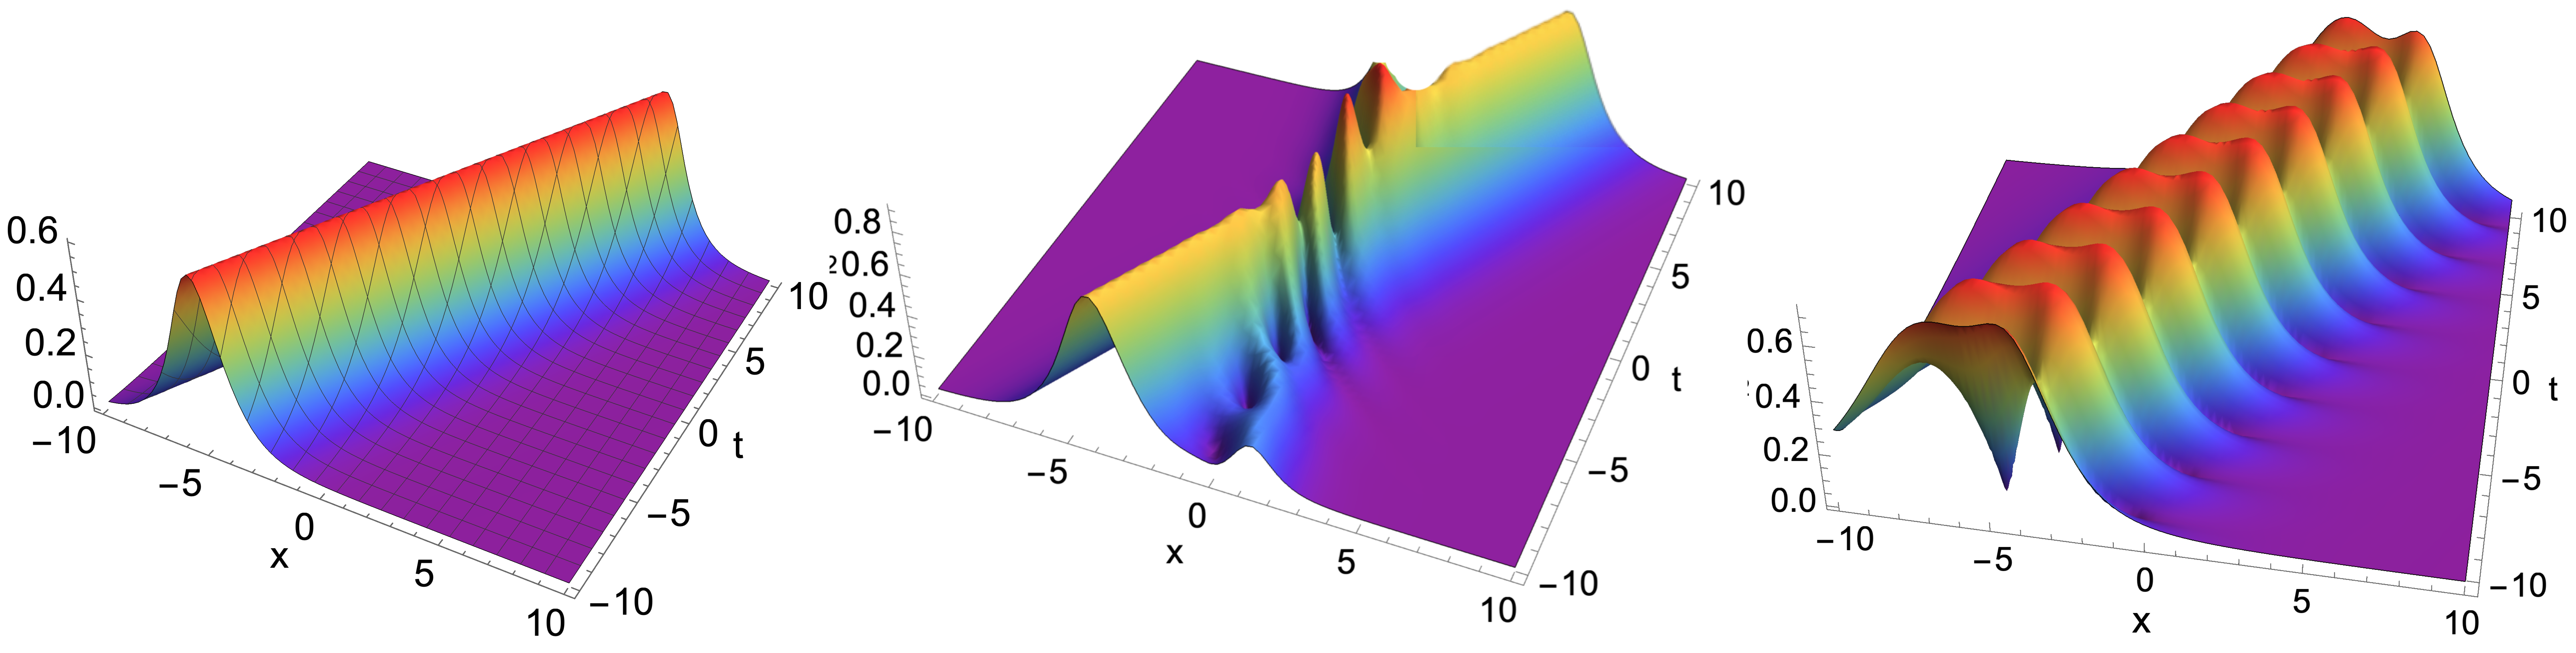
\includegraphics[width=0.9270\linewidth]{figure-Sakkaravarthi.png} 
  \caption{The dynamics of (a) single bright soliton, (b) two-soliton elastic interaction, (c) soliton molecule leading to breather formation.}\label{fig:example}
\end{figure}

%\noindent {\small Acknowledgment: The research is supported through Young Scientist Training (YST) project by APCTP.}

%\end{document}


\end{englisharticle}

 \begin{englisharticle}


\iffalse

% !TeX spellcheck = en_US
%%%%%%%%%%%%%%%%%%%%%%%%%%%%%%%%%%%%%%%%%%%%%%%%%%%%%%%%%%%%%%%%%%%%%%%%
%
% This is the template file for the 6th International conference
% NONLINEAR ANALYSIS AND EXTREMAL PROBLEMS
% June 25-30, 2018
% Irkutsk, Russia
%
%%%%%%%%%%%%%%%%%%%%%%%%%%%%%%%%%%%%%%%%%%%%%%%%%%%%%%%%%%%%%%%%%%%%%%%%
% The preparation of the article is based on the standard llncs class
% (Lecture Notes in Computer Sciences), which is adjusted with style
% file of the conference.
%
% There are two ways of compilation of the file into PDF
% 1. Use pdfLaTeX (pdflatex), (LaTeX+DVIPS will not work);
% 2. Use LuaLaTeX (XeLaTeX will work too).
% When using LuaLaTeX You will need TTF or OTF CMU fonts
% (Computer Modern Unicode). The fonts are installed with 'cm-unicode' package in
% a distribution of LaTeX % (https://www.ctan.org/tex-archive/fonts/cm-unicode),
% either by downloading and installing these fonts system wide, the address of their page is
% http://canopus.iacp.dvo.ru/%7Epanov/cm-unicode/
% The second option won't work in XeLaTeX.
%
% For MiKTeX (LaTeX distribution for Windows),
%  1. Package 'cm-unicode' is installed manually with the MiKTeX administration Console.
%  2. For the compilation of this example, namely, the stub figure, one will also need to
% download package 'pgf' manually. This package uses in the popular
% package tikz.
%  3. Tests showed that the rest of the required packages MiKTeX loads automatically (if
%     it is allowed). The 'auto download' option is
%     configured in 'Settings' section in MiKTeX Console.
%
%
% The easiest way to compile an article is to use pdfLaTeX, but
% the final layout of the book will be compiled with LuaLaTeX,
% as a result will be of better quality thanks to the package 'microtype' and
% use vector OTF instead of standard raster fonts of pdfLaTeX.
%
% In the case of questions and problems with the article compilation,
% write letters to e-mail: eugeneai@irnok.net, Cherkashin Evgeny.
%
% New version of the correcting style file will be available at the website:
%     https://github.com/eugeneai/nla-style
%     file - nla.sty
%
% Further instructions are in the text body of the template. The template itself
% is an article example.
%
% The LaTeX2e format is used!

% 12 points font size is used.
\documentclass[12pt]{llncs}

% The correcting style file is added.
\usepackage{todonotes}

\usepackage{nla} % This package is needed for compiling
                 % this template, it should be removed
                 % from your article.

% Many popular packages (amsXXX, graphicx, etc.) are already imported in the style file.
% If there is a conflict with your packages, try disabling them and compile
% the text.
%
% It would be convenient in the layout of the proceedings if the file names
% of the figures of different authors do not clash.
% To minimize the clash, the drawings can be placed in a separate subfolder
% named after the author or the title of the paper.
%
% \graphicspath{{ivanov-petrov-pics/}} % specifies the folder with images in png, pdf formats.
% or
% \graphicspath{{great-problem-solving-paper-pics/}}.

\begin{document}

 

% Text should be formatted in accordance with the 'article' class, using extensions like
% AMS.
%
\fi

\title{A scheme for numerical  solving of a bilinear optimal impulsive control problem with intermediate state constraints\thanks{This work is financially supported by the Ministry of Education and Science of the Russian Federation (state registration No.~121041300060-4.}}
\author{Olga Samsonyuk}
\institute{ISDCT SB RAS, Irkutsk, Russia\\
  \email{olga.samsonyuk@icc.ru}
}
% etc

\maketitle

\begin{abstract}
This note addresses a  scheme for numerical solving of a bilinear  optimal impulsive control problem with intermediate state constraints.  The scheme is based on optimality conditions using compound monotone functions of the Lyapunov type.

\keywords{impulsive control,  optimality conditions, numerical scheme}
\end{abstract}

Let us consider the optimal impulsive control problem  $(P)$: $\ J=l(q)\rightarrow \min,$
\begin{align}
& d{x}_1(t)=f_1(t)dt+\big(ax_2(t)+b\big)\mu_1(t),  
 \ \  d{x}_2(t)=f_2(t)dt+\big(cx_1(t)+d\big)\mu_2(t),  
 \label{nla3}\\ 
 &  x_1(0)=x_{10}, \  x_2(0)=x_{20}, \ \   q_j\in Q_j,\  j=0,\ldots,N   .\label{nla5}
\end{align}
Here, $T=[0,t_1]$ is a given time interval,  $\mu=(\mu_1, \mu_2)$ is a nonnegative bounded Borel measure on $T$,  $x_1(\cdot)$,  $x_2(\cdot)$,  $V(\cdot)$ are right continuous on $(0,t_1]$ and have bounded total variation on $T$,    $(\theta_0,\theta_1,\ldots,\theta_N)$ are given points such that $0=\theta_0<\theta_1<\ldots<\theta_N=t_1$, $q=\big(q_0,q_1,\ldots,q_N\big)$, where $ q_j=\big(x_1(\theta_j),x_2(\theta_j),V(\theta_j)\big)$, $j=0,\ldots,N$. The constraint sets $Q_j$, $j=0,\ldots,N$, are compact subsets from ${\mathbb R}^3$. The solution's concept to (\ref{nla3}) is given in \cite{samnla2}.

We propose a compound Lyapunov type function described by a continuous  piecewise smooth function $\varphi(t,x_1,x_2,V;t_0,y_{10},y_{20})$ such that $\varphi = \big\{ \varphi_i\big\}_{i=1,\ldots,7} ,$ where functions $\varphi_i$ are defined on   domains with disjoint interiors. The function $\varphi$ is such that: (i)    $\varphi_i$, $i=1,\ldots,7,$ are strongly monotone with respect to  (\ref{nla3})  on every interval $(\theta_{j-1},\theta_j]$, $j=\overline{1,N}$  ($t_0=\theta_{j-1}$); (ii)    $\varphi$ is weakly premonotone with respect to    (\ref{nla3}) on   $(\theta_{j-1},\theta_j]$, $j=\overline{1,N}$, and satisfies the condition
$
\big\{(x_1,x_2)\ |\  \varphi(t_0,x_1,x_2,0;t_0,y_{10},y_{20})\leq 0\big\}=\{y_{10},y_{20}\}.
$ 
The function $\varphi$ gives an approximation of the reachable set and allows us to use the optimality conditions with compound monotone functions of the Lyapunov type   from   \cite{samnla2,samnla1}. Based on these conditions, we propose a scheme for numerical solving of the problem $(P)$.

\begin{thebibliography}{5}
%\bibitem{MilRub2013nla3} Miller  B.M.,   Rubinovich E.Ya.  Discontinuous solutions in the optimal control problems and their representation by singular space-time transformations. Autom. Remote Control. 2013. Vol. 74. Pp. 1969--2006.
\bibitem{samnla2} Samsonyuk O.N., Sorokin S.P. Optimality conditions for impulsive
processes with intermediate state constraints.  The 15th International Conference on
Stability and Oscillations of Nonlinear Control Systems (Pyatnitskiy's Conference)
(STAB), Moscow, Russia, 3--5  June 2020.  IEEE, 2020.  %DOI: 10.1109/STAB49150.2020.9140658
\bibitem{samnla1} Samsonyuk O.N. Optimality conditions for optimal impulsive control
problems with multipoint state constraints. Journal of Global Optimization. 2020. Vol.
76, no. 3. Pp. 625--644. %DOI: 10.1007/s10898-019-00868-w 
\end{thebibliography}


%\end{document}

%%% Local Variables:
%%% mode: latex
%%% TeX-master: t
%%% End:

\end{englisharticle}


\begin{englishtitle} % Настраивает LaTeX на использование английского языка
% Этот титульный лист верстается аналогично.
\title{On a property of continuous dependence of sets\\ in the space of measures}
% First author
\author{Dmitrii Serkov\inst{}
  \and
  Alexander Chentsov\inst{}
}
\institute{Krasovskii institute of mathematics and mechanics, Yekaterinburg, RF\\
  \email{serkov@imm.uran.ru}, \email{chentsov@imm.uran.ru}}
% etc

\maketitle

\begin{abstract}
With the aim of applying to program constructions in the theory of differential games and other guarantee optimization problems, we study the dependence of the set of Borel measures on the product $X\times Y$ of metric compact sets on their marginals from some $*$-weak compact set of measures on $X$.
The continuity of such a dependence in the Hausdorff metric generated by the $*$-weak metric on the union of the specified sets of Borel measures is shown to be continuous under varying marginals in the $*$-weak compact set.
\keywords{Borel measure, Hausdorff metric} % в конце списка точка не ставится
\end{abstract}
\end{englishtitle}

\iffalse

%%%%%%%%%%%%%%%%%%%%%%%%%%%%%%%%%%%%%%%%%%%%%%%%%%%%%%%%%%%%%%%%%%%%%%%%
%
%  This is the template file for the 6th International conference
%  NONLINEAR ANALYSIS AND EXTREMAL PROBLEMS
%  June 25-30, 2018
%  Irkutsk, Russia
%
%%%%%%%%%%%%%%%%%%%%%%%%%%%%%%%%%%%%%%%%%%%%%%%%%%%%%%%%%%%%%%%%%%%%%%%%

%  Верстка статьи осуществляется на основе стандартного класса llncs
%  (Lecture Notes in Computer Sciences), который корректируется стилевым
%  файлом конференции.
%
%  Скомпилировать файл в PDF можно двумя способами:
%  1. Использовать pdfLaTeX (pdflatex), (LaTeX+DVIPS не работает);
%  2. Использовать LuaLaTeX (XeLaTeX будет работать тоже).
%  При использовании LuaLaTeX потребуются TTF- или OTF-шрифты CMU
%  (Computer Modern Unicode). Шрифты устанавливаются либо пакетом
%  дистрибутива LaTeX cm-unicode
%              (https://www.ctan.org/tex-archive/fonts/cm-unicode),
%  либо загрузкой и установкой в операционной системе, адрес страницы:
%              http://canopus.iacp.dvo.ru/%7Epanov/cm-unicode/
%  Второй вариант не будет работать в XeLaTeX.
%
%  В MiKTeX (дистрибутив LaTeX для ОС Windows):
%  1. Пакет cm-unicode устанавливается вручную в программе MiKTeX Console.
%  2. Для верстки данного примера, а именно, картинки-заглушки необходимо,
%     также вручную, загрузить пакет pgf. Этот пакет используется популярным
%     пакетом tikz.
%  3. Тест показал, что остальные пакеты MiKTeX грузит автоматически (если
%     ему разрешено автоматически грузить пакеты). Режим автозагрузки
%     настраивается в разделе Settings в MiKTeX Console.
%
%
%  Самый простой способ сверстать статью - использовать pdfLaTeX, но
%  окончательный вариант верстки сборника будет собран в LuaLaTeX,
%  так как результат получится лучшего качества, благодаря пакету microtype и
%  использованию векторных шрифтов OTF вместо растровых pdfLaTeX.
%
%  В случае возникновения вопросов и проблем с версткой статьи,
%  пишите письма на электронную почту: eugeneai@irnok.net, Черкашин Евгений.
%
%  Новые варианты корректирующего стиля будут доступны на сайте:
%        https://github.com/eugeneai/nla-style
%        файл - nla.sty
%
%  Дальнейшие инструкции - в тексте данного шаблона. Он одновременно
%  является примером статьи.
%
%  Формат LaTeX2e!

\documentclass[12pt]{llncs}  % Необходимо использовать шрифт 12 пунктов.

% При использовании pdfLaTeX добавляется стандартный набор русификации babel.
% Если верстка производится в LuaLaTeX, то следующие три строки надо
% закомментировать, русификация будет произведена в корректирующем стиле автоматом.
\usepackage{iftex}

\ifPDFTeX
\usepackage[T2A]{fontenc}
\usepackage[utf8]{inputenc} % Кодировка utf-8, cp1251 и т.д.
\usepackage[english,russian]{babel}
\fi

% Для верстки в LuaLaTeX текст готовится строго в utf-8!

% В операционной системе Windows для редактирования в кодировке utf-8
% можно использовать программы notepad++ https://notepad-plus-plus.org/,
% techniccenter http://www.texniccenter.org/,
% SciTE (самая маленькая по объему программа) http://www.scintilla.org/SciTEDownload.html
% Подойдет также и встроенный в свежий дистрибутив MiKTeX редактор
% TeXworks.

% Добавляется корректирующий стилевой файл строго после babel, если он был включен.
% В параметре необходимо указать russian, что установит не совсем стандартные названия
% разделов текста, настроит переносы для русского языка как основного и т.п.

\usepackage{todonotes} % Этот пакет нужен для верстки данного шаблона, его
                       % надо убрать из вашей статьи.

\usepackage[russian]{nla}

% Многие популярные пакеты (amsXXX, graphicx и т.д.) уже импортированы в корректирующий стиль.
% Если возникнут конфликты с вашими пакетами, попробуйте их отключить и сверстать
% текст как есть.
%
%


% Было б удобно при верстке сборника, чтобы названия рисунков разных авторов не пересекались.
% Чтоб минимизировать такое пересечение, рисунки можно поместить в отдельную подпапку с
% названием - фамилией автора или названием статьи.
%
% \graphicspath{{ivanov-petrov-pics/}} % Указание папки с изображениями в форматах png, pdf.
% или
% \graphicspath{{great-problem-solving-paper-pics/}}.


\begin{document}

% Текст оформляется в соответствии с классом article, используя дополнения
% AMS.
%
\fi

\title{Об одном свойстве непрерывной зависимости множеств\\ в пространстве мер}%\thanks{Работа выполнена при поддержке РФФИ (РНФ, другие фонды), проект \textnumero~00-00-00000.}
% Первый автор
\author{Д.~А.~Серков\inst{}  % \inst ставит циферку над автором.
  \and  % разделяет авторов, в тексте выглядит как запятая.
% Второй автор
А.~Г.~Ченцов\inst{}
  \and
} % обязательное поле

% Аффилиации пишутся в следующей форме, соединяя каждый институт при помощи \and.
\institute{ИММ УрО РАН, Екатеринбург, РФ\\
  \email{serkov@imm.uran.ru},  \email{chentsov@imm.uran.ru}
}

\maketitle

\begin{abstract}
С целью применения к программным конструкциям в теории дифференциальных игр и других задачах оптимизации гарантии, изучается зависимость множества борелевских мер на произведении $X\times Y$ метрических компактов от их маргиналов из некоторого $*$-слабого компакта мер на $X$.
Показана непрерывности такой зависимости в метрике Хаусдорфа, порождённой $*$-слабой метрикой на объединении указанных множеств борелевских мер, при изменении маргиналов в $*$-слабом компакте.

\keywords{борелевская мера, метрика Хаусдорфа} % в конце списка точка не ставится
\end{abstract}

%\section{Основные результаты} % не обязательное поле

Рассматривается декартово произведение $X\times Y$ двух непустых метрических компактов $X$, $Y$ с $\sigma$-алгебрами своих борелевских подмножеств.
На компакте $X$ задан непустой компакт $M$ борелевских (неотрицательных) мер в относительной *-слабой топологии (в этом случае каждая борелевская мера регулярна (см., например, \cite[гл. 1. \S1]{Bil})).
Каждой мере $\mu$ из этого компакта сопоставляется множество $\mathfrak{N}_\mu$ всех борелевских мер на произведении компактов $X\times Y$ с общим маргинальным распределением в виде указанной меры $\mu$;
данное множество назовем программой, отвечающей данной мере $\mu$ на метрическом компакте $X$.
Пространство знакопеременных борелевских мер на произведении $X\times Y$ оснащаем *-слабой топологией.
Объединение всех программ оказывается *-слабо замкнутым и сильно ограниченным в силу (*-слабой) компактности множества мер $M$.
Поскольку пространство непрерывных функций на произведении метрических компактов сепарабельно, то (*-слабо компактное) объединение программ, рассматриваемое как подпространство пространства (знакопеременных) борелевских мер на $X\times Y$, метризуемо \cite[Теорема 1.3.12]{Warga}.
Фиксируя некоторую метрику $\rho$, порождающую указанную относительную $*$-слабую топологию на объединении программ, получаем метрический компакт, на непустых замкнутых подмножествах которого вводим метрику Хаусдорфа.
В частности, оценивая в этой метрике различие программ $\mathfrak{N}_\mu$, $\mu\in M$, показываем, что зависимость упомянутых программ $\mathfrak{N}_\mu$ от порождающих эти программы маргинальных мер $\mu\in M$ непрерывна.

Данное утверждение существенно обобщает положение \cite[Лемма П.2]{Chentsov}, использовавшееся в конструкциях решения регулярных дифференциальных игр \cite[глава VII]{KraSub};
добавим к этому свойство непрерывной зависимости пучков обобщённых траекторий в дифференциальных играх при изменении порождающих эти пучки управлений мер одного из игроков \cite{Chentsov-VINITI}.
Свойства такого рода существенны в конструкциях \cite{KraSub} решения нелинейных дифференциальных игр, использующих понятие программного максимина.
Данные конструкции, в свою очередь, являются глубоким развитием понятия регулярности для линейных дифференциальных игр, предложенного в  \cite{Kra}.



% Рисунки и таблицы оформляются по стандарту класса article. Например,

% Современные издательства требуют использовать кавычки-елочки << >>.

% В конце текста можно выразить благодарности, если этого не было
% сделано в ссылке с заголовка статьи, например,
%Работа выполнена при поддержке РФФИ (РНФ, другие фонды), проект \textnumero~00-00-00000.
%

% Список литературы оформляется подобно ГОСТ-2008.
% Примеры оформления находятся по этому адресу -
%     https://narfu.ru/agtu/www.agtu.ru/fad08f5ab5ca9486942a52596ba6582elit.html
%

\begin{thebibliography}{9} % или {99}, если ссылок больше десяти.

\bibitem{Bil}Биллингсли П. Сходимость вероятностных мер. М.: Наука, 1977.

\bibitem{Warga} Варга Д. Оптимальное управление дифференциальными и функциональными уравнениями. М.: Наука, 1977.

\bibitem{Chentsov} Ченцов А. Г. Об одной игровой задаче управления на минимакс // Изв. АН СССР. Сер. Техн. кибернетика. 1975. № 1. С. 39--46.

\bibitem{KraSub} Красовский Н. Н., Субботин A. И. Позиционные дифференциальные игры. М.: Наука. 1974.

\bibitem{Chentsov-VINITI} Ченцов A. Г. Метод программных итераций для дифференциальной игры сближения–уклонения // Уральский политехнический институт им. С.М.Кирова. Свердловск. Рукопись депонирована в ВИНИТИ 1933–79. 1979.

\bibitem{Kra} Красовский Н. Н. Игровые задачи о встрече движений. М.: Наука, 1970.

\end{thebibliography}

% После библиографического списка в русскоязычных статьях необходимо оформить
% англоязычный заголовок.




%\end{document}

%%% Local Variables:
%%% mode: latex
%%% TeX-master: t
%%% End:


\begin{englishtitle} % Настраивает LaTeX на использование английского языка
% Этот титульный лист верстается аналогично.
\title{On the Solution of the Hamilton-Jacobi Equation with State Constraints Given by Zeros of the Coefficients at the Exponential Terms of the Hamiltonian}
% First author
\author{Lyubov Shagalova}
\institute{ IMM UrB  RAS, Yekaterinburg, Russia\\
  \email{shag@imm.uran.ru}}
  
\maketitle

\begin{abstract}
The Cauchy problem for the Hamilton-Jacobi equation with a Hamiltonian depending on the state and momentum variables is considered. In this case, the dependence on the momentum  is exponential. The state space is one-dimensional. The problem is considered in the strip determined by zeros of the monotone functions of the state variable which are the coefficients at the exponential terms of the Hamiltonian. The existence and uniqueness theorem for the viscosity solution of the problem under consideration is proved. 

\keywords{Hamilton-Jacobi equation, viscosity solution, state constraints, method of characteristics} % в конце списка точка не ставится
\end{abstract}
\end{englishtitle}


\iffalse
%%%%%%%%%%%%%%%%%%%%%%%%%%%%%%%%%%%%%%%%%%%%%%%%%%%%%%%%%%%%%%%%%%%%%%%%
%
%  This is the template file for the 6th International conference
%  NONLINEAR ANALYSIS AND EXTREMAL PROBLEMS
%  June 25-30, 2018
%  Irkutsk, Russia
%
%%%%%%%%%%%%%%%%%%%%%%%%%%%%%%%%%%%%%%%%%%%%%%%%%%%%%%%%%%%%%%%%%%%%%%%%

%  Верстка статьи осуществляется на основе стандартного класса llncs
%  (Lecture Notes in Computer Sciences), который корректируется стилевым
%  файлом конференции.
%
%  Скомпилировать файл в PDF можно двумя способами:
%  1. Использовать pdfLaTeX (pdflatex), (LaTeX+DVIPS не работает);
%  2. Использовать LuaLaTeX (XeTeX не будет работать).
%  При использовании LuaLaTeX потребуются TTF- или OTF-шрифты CMU
%  (Computer Modern Unicode). Шрифты устанавливаются либо пакетом
%  дистрибутива LaTeX cm-unicode
%              (https://www.ctan.org/tex-archive/fonts/cm-unicode),
%  либо загрузкой и установкой в операционной системе, адрес страницы:
%  http://canopus.iacp.dvo.ru/%7Epanov/cm-unicode/
%
%  В MiKTeX (дистрибутив LaTeX для ОС Windows):
%  1. Пакет cm-unicode устанавливается вручную в программе MiKTeX Console.
%  2. Для верстки данного примера, а именно, картинки-заглушки необходимо,
%     также вручную, загрузить пакет pgf. Этот пакет используется популярным
%     пакетом tikz.
%  3. Тест показал, что остальные пакеты MiKTeX грузит автоматически (если
%     ему разрешено автоматически грузить пакеты). Режим автозагрузки
%     настраивается в разделе Settings в MiKTeX Console.
%
%
%  Самый простой способ сверстать статью - использовать pdfLaTeX, но
%  окончательный вариант верстки сборника будет собран в LuaLaTeX,
%  так как результат получится лучшего качества.
%
%  В случае возникновения вопросов и проблем с версткой статьи,
%  пишите письма на электронную почту: eugeneai@irnko.net, Черкашин Евгений
%
%  Новые варианты корректирующего стиля будут доступны на сайте:
%        https://github.com/eugeneai/nla-style
%        файл - nla.sty
%
%  Дальнейшие инструкции - в тексте данного шаблона. Он одновременно
%  является примером статьи.
%
%  Формат LaTeX2e!

\documentclass[12pt]{llncs}  % Необходимо использовать шрифт 12 пунктов.

% При использовании pdfLaTeX добавляется стандартный набор русификации babel.
% Если верстка производится в LuaLaTeX, то следующие три строки надо
% закомментировать, русификация будет произведена в корректирующем стиле автоматом.
\usepackage[T2A]{fontenc}
\usepackage[cp1251]{inputenc} % Кодировка utf-8, win1251 (cp1251) не тестировалась.
\usepackage[english,russian]{babel}

% Для верстки в LuaLaTeX текст готовится строго в utf-8!

% В операционной системе Windows для редактирования в кодировки utf-8
% можно использовать программы notepad++ https://notepad-plus-plus.org/,
% techniccenter http://www.texniccenter.org/,
% SciTE (самая маленькая по объему программа) http://www.scintilla.org/SciTEDownload.html
% Подойдет также и встроенный в свежий дистрибутив MiKTeX редактор
% TeXworks.

% Добавляется корректирующий стилевой файл строго после babel, если он был включен.
% В параметре необходимо указать russian, что установит не совсем стандартные названия
% разделов текста, настроит переносы для русского языка как основного и т.п.

\usepackage{todonotes} % Удрать из вашей статьи, нужен для верстки данного шаблона.

\usepackage[russian]{nla}

% Многие популярные пакеты (amsXXX, graphicx и т.д.) уже импортированы в корректирующий стиль.
% Если возникнут конфликты с вашими пакетами, попробуйте их отключить и сверстать
% текст как есть.
%
%


% Было б удобно при верстке сборника, чтобы названия рисунков разных авторов не пересекались.
% Чтоб минимизировать такое пересечение, рисунки можно поместить в отдельную подпапку с
% названием - фамилией автора или названием статьи.
%
% \graphicspath{{ivanov-petrov-pics/}} % Указание папки с изображениями в форматах png, pdf.
% или
% \graphicspath{{great-problem-solving-paper-pics/}} % Указание папки с изображениями в форматах png, pdf.


\begin{document}

% Текст оформляется в соответствии с классом article, используя дополнения
% AMS.
%
\fi

\title{О решении уравнения Гамильтона -- Якоби с фазовыми ограничениями, задаваемыми нулями коэффициентов при экспоненциальных слагаемых гамильтониана}%\thanks{Работа выполнена при поддержке РФФИ (РНФ, другие фонды), проект \textnumero~00-00-00000.}}
% Первый автор
\author{Л.~Г.~Шагалова%\inst{1}  % \inst ставит циферку над автором.
  %\and  % разделяет авторов, в тексте выглядит как запятая.
% Второй автор
 % И.~О.~Фамилия\inst{2}
  %\and
% Третий автор
 % И.~О.~Фамилия\inst{1}
} % обязательное поле

% Аффилиации пишутся в следующей форме, соединяя каждый институт при помощи \and.
\institute{ИММ УрО РАН, Екатеринбург, Россия\\
  \email{shag@imm.uran.ru}
  %\and   % Разделяет институты и присваивает им номера по порядку.
%Институт (название в краткой форме), Город, Страна\\
%\email{email@examle.com}
% \and Другие авторы...
}

\maketitle

\begin{abstract}
Рассматривается задача Коши для уравнения Гамильтона -- Якоби с гамильтонианом, зависящим от фазовой и импульсной переменной.
При этом зависимость от импульсной переменной экспоненциальна. Фазовое пространство одномерно. Задача рассматривается в полосе, определяемой нулями монотонных функций фазовой переменной, которые являются коэффициентами при экспоненциальных слагаемых гамильтониана. Доказана теорема существования и единственности вязкостного решения рассматриваемой задачи.

\keywords{уравнение Гамильтона -- Якоби, вязкостное решение, фазовые ограничения, метод характеристик } % в конце списка точка не ставится
\end{abstract}

Рассматривается задача Коши для уравнения Гамильтона -- Якоби с фазовыми ограничениями следующего вида
\begin{equation}\label{eqn1}
\frac{\partial u}{\partial t} + H\left(x, \frac{\partial u}{\partial x}\right)=0, \quad  t \in (0,T), \, x \in [x_*, x^*]
\end{equation}
\begin{equation}\label{eqn2}
u(0,x)=u_0(x),  \quad x \in R.
\end{equation}
Здесь $T > 0$~-- заданный момент времени, $u_0(\cdot)$~-- непрерывно дифференцируемая функция.

Заданы непрерывно дифференцируемые функции $h(\cdot): R \rightarrow R$, \quad $f(\cdot): R \rightarrow R$, \quad $g(\cdot):R \rightarrow R$. При этом $f(\cdot)$ является строго возрастающей, а $g(\cdot)$ --- cтрого убывающей, и существуют точки $x_*$ и $x^*$, \quad $x_* < x^*$ такие, что
$$
f(x_*)=0, \quad g(x^*)=0.$$

Таким образом, отрезок $[x_*, x^*]$ в (\ref{eqn1}) определяется нулями функций $f(\cdot)$ и $g(\cdot)$. Задача~(\ref{eqn1}), (\ref{eqn2}) рассматривается в случае, когда гамильтониан имеет вид
\begin{equation}\label{hama}
H(x,p)=h(x)+f(x)e^p +g(x)e^{-p}.
\end{equation}
Поскольку на отрезке $[x_*, x^*]$ функции $f(\cdot)$ и $g(\cdot)$ неотрицательны, гамильтониан (\ref{hama}) является выпуклым по импульсной переменной $p$.

Задачи с экспоненциальной зависимостью гамильтониана нетипичны для теории уравнений Гамильтона -- Якоби. Вместе с тем, такие задачи возникают в прикладных исследованиях (см., например, \cite{Saak}). При этом для таких задач не выполнены известные условия, для которых доказаны теоремы существования вязкостных \cite{Crandall} решений. Для ряда подобных задач вязкостных решений не существует, поэтому приходится вводить новые обобщенные решения \cite{SubbShag}.

Для задачи (\ref{eqn1}),(\ref{eqn2}),(\ref{hama}) доказана теорема существования и единственности вязкостного решения. Доказательство теоремы базируется на решении задач вариационного исчисления с подвижными границами \cite{Clarke}, исследовании характеристической системы уравнения (\ref{eqn1}), (\ref{hama}) с начальным условием (\ref{eqn2}) и применении метода обобщенных характеристик \cite{Subbotina}.



% Современные издательства требуют использовать кавычки-елочки << >>.


% Список литературы оформляется подобно ГОСТ-2008.
% Примеры оформления находятся по этому адресу -
%     https://narfu.ru/agtu/www.agtu.ru/fad08f5ab5ca9486942a52596ba6582elit.html
%

\begin{thebibliography}{9} % или {99}, если ссылок больше десяти.

\bibitem{Saak} Saakian~D.B., Rozanova~O., Akmetzhanov~A. Dynamics of the Eigen and the Crow-Kimura models for molecular
evolution. Physical Review E. 2008. Vol~78. 041908.

\bibitem{Crandall} Crandall~M.G., Lions~P.-L. Viscosity solutions of Hamilton–Jacobi equations. Trans. Amer. Math. Soc.  1983. Vol.~277, no.~1. P.~1--42.

\bibitem{SubbShag} Cубботина~Н.Н., Шагалова~Л.Г. О решении задачи Коши для уравнения Гамильтона~-– Якоби с фазовыми ограничениями~// Труды Института математики и механики УрО РАН. 2011.  Т.~17, \textnumero~2. C.~191--208.
    
\bibitem{Clarke} Clarke~F.H. Tonelli’s regurarity theory in the calculus of variations: Recent progress. Optimization and Related Fields. Lecture Notes in Mathematics. 1986. Vol.~1190. P.~163--179.
    
\bibitem{Subbotina} Subbotina~N.N. The method of characteristics for Hamilton–Jacobi equation and its applications in dynamical optimization. Modern Mathematics and its Applications.  2004.  Vol.~20. P.~2955--3091.
    

\end{thebibliography}

% После библиографического списка в русскоязычных статьях необходимо оформить
% англоязычный заголовок.



%\end{document}

%%% Local Variables:
%%% mode: latex
%%% TeX-master: t
%%% End:


\begin{englishtitle} % Настраивает LaTeX на использование английского языка
% Этот титульный лист верстается аналогично.
\title{Fluid Storage Control with a Proportional-integrally Differentiating Solver}
% First author
\author{E.~R.~Shaihiev\inst{1}
  \and
  A.~D.~Nizamova\inst{2}
 }
\institute{USATU, Ufa, Russia\\
  \email{erik08082002@mail.ru}
  \and
Mavlyutov Institute of Mechanics, Ufa Investigation Center, RAS, Russia\\
\email{adeshka@yandex.ru}}
% etc

\maketitle

\begin{abstract}
For water and oil the PID-controller coefficients responsible for the operation of the outlet valve were found, an interface was created for controlling, automating and optimizing a given process in the open software tool "WinCC OA" by SIEMENS.

\keywords{proportional-integrally differentiating solver, proportional-integrally differentiating coefficient, fluid} % в конце списка точка не ставится
\end{abstract}
\end{englishtitle}

\iffalse

%%%%%%%%%%%%%%%%%%%%%%%%%%%%%%%%%%%%%%%%%%%%%%%%%%%%%%%%%%%%%%%%%%%%%%%%
%
%  This is the template file for the 6th International conference
%  NONLINEAR ANALYSIS AND EXTREMAL PROBLEMS
%  June 25-30, 2018
%  Irkutsk, Russia
%
%%%%%%%%%%%%%%%%%%%%%%%%%%%%%%%%%%%%%%%%%%%%%%%%%%%%%%%%%%%%%%%%%%%%%%%%

%  Верстка статьи осуществляется на основе стандартного класса llncs
%  (Lecture Notes in Computer Sciences), который корректируется стилевым
%  файлом конференции.
%
%  Скомпилировать файл в PDF можно двумя способами:
%  1. Использовать pdfLaTeX (pdflatex), (LaTeX+DVIPS не работает);
%  2. Использовать LuaLaTeX (XeLaTeX будет работать тоже).
%  При использовании LuaLaTeX потребуются TTF- или OTF-шрифты CMU
%  (Computer Modern Unicode). Шрифты устанавливаются либо пакетом
%  дистрибутива LaTeX cm-unicode
%              (https://www.ctan.org/tex-archive/fonts/cm-unicode),
%  либо загрузкой и установкой в операционной системе, адрес страницы:
%              http://canopus.iacp.dvo.ru/%7Epanov/cm-unicode/
%  Второй вариант не будет работать в XeLaTeX.
%
%  В MiKTeX (дистрибутив LaTeX для ОС Windows):
%  1. Пакет cm-unicode устанавливается вручную в программе MiKTeX Console.
%  2. Для верстки данного примера, а именно, картинки-заглушки необходимо,
%     также вручную, загрузить пакет pgf. Этот пакет используется популярным
%     пакетом tikz.
%  3. Тест показал, что остальные пакеты MiKTeX грузит автоматически (если
%     ему разрешено автоматически грузить пакеты). Режим автозагрузки
%     настраивается в разделе Settings в MiKTeX Console.
%
%
%  Самый простой способ сверстать статью - использовать pdfLaTeX, но
%  окончательный вариант верстки сборника будет собран в LuaLaTeX,
%  так как результат получится лучшего качества, благодаря пакету microtype и
%  использованию векторных шрифтов OTF вместо растровых pdfLaTeX.
%
%  В случае возникновения вопросов и проблем с версткой статьи,
%  пишите письма на электронную почту: eugeneai@irnok.net, Черкашин Евгений.
%
%  Новые варианты корректирующего стиля будут доступны на сайте:
%        https://github.com/eugeneai/nla-style
%        файл - nla.sty
%
%  Дальнейшие инструкции - в тексте данного шаблона. Он одновременно
%  является примером статьи.
%
%  Формат LaTeX2e!

\documentclass[12pt]{llncs}  % Необходимо использовать шрифт 12 пунктов.

% При использовании pdfLaTeX добавляется стандартный набор русификации babel.
% Если верстка производится в LuaLaTeX, то следующие три строки надо
% закомментировать, русификация будет произведена в корректирующем стиле автоматом.
\usepackage{iftex}

\ifPDFTeX
\usepackage[T2A]{fontenc}
\usepackage[utf8]{inputenc} % Кодировка utf-8, cp1251 и т.д.
\usepackage[english,russian]{babel}
\fi

% Для верстки в LuaLaTeX текст готовится строго в utf-8!

% В операционной системе Windows для редактирования в кодировке utf-8
% можно использовать программы notepad++ https://notepad-plus-plus.org/,
% techniccenter http://www.texniccenter.org/,
% SciTE (самая маленькая по объему программа) http://www.scintilla.org/SciTEDownload.html
% Подойдет также и встроенный в свежий дистрибутив MiKTeX редактор
% TeXworks.

% Добавляется корректирующий стилевой файл строго после babel, если он был включен.
% В параметре необходимо указать russian, что установит не совсем стандартные названия
% разделов текста, настроит переносы для русского языка как основного и т.п.

\usepackage{todonotes} % Этот пакет нужен для верстки данного шаблона, его
                       % надо убрать из вашей статьи.

\usepackage[russian]{nla}

% Многие популярные пакеты (amsXXX, graphicx и т.д.) уже импортированы в корректирующий стиль.
% Если возникнут конфликты с вашими пакетами, попробуйте их отключить и сверстать
% текст как есть.
%
%


% Было б удобно при верстке сборника, чтобы названия рисунков разных авторов не пересекались.
% Чтоб минимизировать такое пересечение, рисунки можно поместить в отдельную подпапку с
% названием - фамилией автора или названием статьи.
%
% \graphicspath{{ivanov-petrov-pics/}} % Указание папки с изображениями в форматах png, pdf.
% или
% \graphicspath{{great-problem-solving-paper-pics/}}.


\begin{document}

% Текст оформляется в соответствии с классом article, используя дополнения
% AMS.
%
\fi

\title{Контроль хранилища жидкости при помощи ПИД-регулятора}
% Первый автор
\author{Э.~Р.~Шайхиев\inst{1}  % \inst ставит циферку над автором.
  \and  % разделяет авторов, в тексте выглядит как запятая.
% Второй автор
  А.~Д.~Низамова\inst{2}
  \and
} % обязательное поле

% Аффилиации пишутся в следующей форме, соединяя каждый институт при помощи \and.
\institute{УГАТУ, Уфа, Россия \\
  \email{erik08082002@mail.ru}
  \and   % Разделяет институты и присваивает им номера по порядку.
ИМех УФИЦ РАН, Уфа, Россия\\
  \email{adeshka@yandex.ru}
% \and Другие авторы...
}

\maketitle

\begin{abstract}
Для воды и нефти найдены коэффициенты ПИД-регулятора, отвечающие за работу выходного клапана, создан интерфейс для контролирования, автоматизации и оптимизации заданного процесса в открытом программном инструменте "WinCC OA” компании SIEMENS.

\keywords{ПИД-регулятор, ПИД-коэффициент, жидкость} % в конце списка точка не ставится
\end{abstract}

%\section{Основные результаты} % не обязательное поле

Рассматривается гидродинамическая система уравнений для модели вязкой жидкости, в которой определяются параметры установившегося прямолинейного потока несжимаемой жидкости.

Для регулирования выходного потока по мере приближения уровня жидкости к заданному уровню для формирования входного сигнала с точным и качественным переходным процессом в автоматических системах управления используют пропорционально-интегрально-дифференцирующий (ПИД) регулятор.

ПИД-регулятор в управляющем контуре использует обратную связь. ПИД-закон регулирования обеспечивает достаточно высокую точность поддержания уровня жидкости. Уровень оттока жидкости рассчитывается по формуле
$$
u(t)=K_p\cdot e(t)+K_i\int_0^te(\tau)d\tau-R_d\cdot\frac{de(t)}{dt},
$$
где пропорциональный $K_p$, интегральный $K_i$, и дифференциальный $K_d$  ПИД-коэффициенты регулирования.

Слагаемое $K_p\cdot e(t)$ прямо пропорционально ошибке $e(t)$ разности установки и измененного значения уровня. Использовние только пропорциональной части зачастую приводит к ошибке между установкой и фактическим значением.

Слагаемое $K_i\int_0^te(\tau)d\tau$ учитывает прошлые значения ошибки и интегрирует их, то есть при помощи интегральной составляющей устраняет остаточную ошибку, возникающую при использовании одной пропорциональной составляющей.

Слагаемое $-R_d\cdot\frac{de(t)}{dt}$ пропорционально скорости изменения уровня с обратным знаком и должно препятствовать резким скачкам уровня, а именно, упреждает ошибку и эффективно стремится уменьшить ее.

Для достижения хорошего качества регулирования необходимо правильно подобрать коэффициенты к установке. Настройка ПИД-регулятора зачастую осуществляется  методом проб и ошибок.  

Для создания программного интерфейса будем пользоваться программой SIMATIC WinCC Open Architecture от компании SIEMENS, находящуюся в открытом доступе. ПИД-регулирование выполняется с использованием глобального скрипта Model.ctl.

С помощью программы выполняется имитация поведения системы резервуаров, контроллеров и прочего.

\begin{thebibliography}{9} % или {99}, если ссылок больше десяти.

\bibitem{Shaihiev_Sherman} Sherman~F.S. Viscous Flow. McGraw-Hill series in mechanical engineering. McGraw-Hill,~1990.

\bibitem{Shaihiev_Murt}	Муртазина~Р.Д., Кудашева~Е.Г., Низамова~А.Д., Сидельникова~Н.А. Дифференциальные уравнения в частных производных второго порядка. Устойчивость течения жидкостей в канале с линейным профилем температуры. М.:~Русайнс,~2021.


\bibitem{Shaihiev_Niza}	Nizamova~A.D., Murtazina~R.D., Kireev~V.N., Urmancheev~S.F. Features of Laminar-Turbulent Transition for the Coolant Flow in a Plane Heat-Exchanger Channel. Lobachevskii Journal of Mathematics. 2021. Vol.~42. \textnumero~9. Pp.~2211--2215.


\end{thebibliography}

% После библиографического списка в русскоязычных статьях необходимо оформить
% англоязычный заголовок.



%\end{document}

%%% Local Variables:
%%% mode: latex
%%% TeX-master: t
%%% End:


 \begin{englisharticle}
\iffalse

%%%%%%%%%%%%%%%%%%%%%%%%%%%%%%%%%%%%%%%%%%%%%%%%%%%%%%%%%%%%%%%%%%%%%%%%
%
% This is the template file for the 6th International conference
% NONLINEAR ANALYSIS AND EXTREMAL PROBLEMS
% June 25-30, 2018
% Irkutsk, Russia
%
%%%%%%%%%%%%%%%%%%%%%%%%%%%%%%%%%%%%%%%%%%%%%%%%%%%%%%%%%%%%%%%%%%%%%%%%
% The preparation of the article is based on the standard llncs class
% (Lecture Notes in Computer Sciences), which is adjusted with style
% file of the conference.
%
% There are two ways of compilation of the file into PDF
% 1. Use pdfLaTeX (pdflatex), (LaTeX+DVIPS will not work);
% 2. Use LuaLaTeX (XeLaTeX will work too).
% When using LuaLaTeX You will need TTF or OTF CMU fonts
% (Computer Modern Unicode). The fonts are installed with 'cm-unicode' package in
% a distribution of LaTeX % (https://www.ctan.org/tex-archive/fonts/cm-unicode),
% either by downloading and installing these fonts system wide, the address of their page is
% http://canopus.iacp.dvo.ru/%7Epanov/cm-unicode/
% The second option won't work in XeLaTeX.
%
% For MiKTeX (LaTeX distribution for Windows),
%  1. Package 'cm-unicode' is installed manually with the MiKTeX administration Console.
%  2. For the compilation of this example, namely, the stub figure, one will also need to
% download package 'pgf' manually. This package uses in the popular
% package tikz.
%  3. Tests showed that the rest of the required packages MiKTeX loads automatically (if
%     it is allowed). The 'auto download' option is
%     configured in 'Settings' section in MiKTeX Console.
%
%
% The easiest way to compile an article is to use pdfLaTeX, but
% the final layout of the book will be compiled with LuaLaTeX,
% as a result will be of better quality thanks to the package 'microtype' and
% use vector OTF instead of standard raster fonts of pdfLaTeX.
%
% In the case of questions and problems with the article compilation,
% write letters to e-mail: eugeneai@irnok.net, Cherkashin Evgeny.
%
% New version of the correcting style file will be available at the website:
%     https://github.com/eugeneai/nla-style
%     file - nla.sty
%
% Further instructions are in the text body of the template. The template itself
% is an article example.
%
% The LaTeX2e format is used!

% 12 points font size is used.
\documentclass[12pt]{llncs}

% The correcting style file is added.
\usepackage{todonotes}

\usepackage{nla} % This package is needed for compiling
                 % this template, it should be removed
                 % from your article.

% Many popular packages (amsXXX, graphicx, etc.) are already imported in the style file.
% If there is a conflict with your packages, try disabling them and compile
% the text.
%
% It would be convenient in the layout of the proceedings if the file names
% of the figures of different authors do not clash.
% To minimize the clash, the drawings can be placed in a separate subfolder
% named after the author or the title of the paper.
%
% \graphicspath{{ivanov-petrov-pics/}} % specifies the folder with images in png, pdf formats.
% or
% \graphicspath{{great-problem-solving-paper-pics/}}.

\begin{document}

% Text should be formatted in accordance with the 'article' class, using extensions like
% AMS.
%

\fi
\title{Tensor Invariants of Dynamical Systems with Dissipation}
% First author
\author{Maxim V.~Shamolin 
}
\institute{Lomonosov Moscow State University, Moscow, Russia\\
  \email{shamolin@rambler.ru,~shamolin@imec.msu.ru}}
% etc

\maketitle

\begin{abstract}
In this work, the complete set of tensor invariants of some classes of dynamic systems on the tangent bundles of a multidimensional
manifold is demonstrated. In this case, force fields are characterized by so-called variable dissipation
and generalize the earlier considered fields.

\keywords{dynamical system, tensor invariants, dissipation, integrability}
\end{abstract}

% at the end of the list, there should be no final dot
%\section{The main results}

In the problems of dynamics, mechanical systems
with many degrees of freedom with dissipation (position
space, multidimensional manifold) are studied.
The tangent bundles of these manifolds become their
phase spaces. Thus, for example, the study of an ndimensional
generalized spherical pendulum in a nonconservative
field of forces leads to a dynamic system
on the tangent bundles of an $(n-1)$-dimensional
sphere, and the metrics of special form on it are
induced by an additional group of symmetry \cite{1}, \cite{2}. In
this case, the dynamic systems describing the motion
of such a pendulum are characterized by alternating
dissipation, and the complete list of the first integrals
is composed of transcendental (in the sense of complex
analysis) functions, which can be expressed
through a finite combination of elementary functions.

Let us also define the class of problems about the
motion of a point over a multidimensional surface, the
metrics on which are induced by the Euclidian metrics
of the overall space. In some cases, it is also possible to
find the complete list of the first integrals composed of
transcendental functions in systems with dissipation.
The results obtained are especially important in the
sense of the presence of just a nonconservative field of
forces in a system.

In this work, the integrability of some classes of
dynamic systems on the tangent bundles of a multidimensional
manifold is demonstrated (for similar studies
on the tangent bundles of two-, three, and fourdimensional
manifolds, see \cite{3}, \cite{4}, \cite{5}). In this case, the force fields are characterized by so-called alternating
dissipation and generalize the fields considered earlier
(see also \cite{6}, \cite{7}). 

% The figures and tables are drawn according to the standard class 'article'.
%\begin{figure}[htb]
 % \centering

% Two picture formats are supported:
%\includegraphics[width=0.7\linewidth]{figure.pdf} % Raster format
%\includegraphics[width=0.7\linewidth]{figure.png} % Vector and raster format
%
% Vector drawings can be drawn in Inkscape editor
% https://inkscape.org/ru/download/
% The usual format of the editor is SVG, so the drawings must be exported in
% PDF or PNG (with a resolution of minimum 150 dpi, and maximum of 300 dpi).
%  \begin{center}
%    \missingfigure[figwidth=0.7\linewidth]{Remove me from the article!} \end{center}
%  \caption{Caption of the figure}\label{fig:example}
%\end{figure}

% At the end of the text, acknowledgments are expressed, if you haven't
% made a footnote from the title. For example, we can write
%The research is carried on with support of RFBR (RNF, other funds), project No.~00-00-00000.

\begin{thebibliography}{9} % or {99}, if there is more than ten references.
\bibitem{1} Shamolin M.V. New Case of Integrability in the Dynamics of a Multidimensional Solid in a Nonconservative Field. Doklady Physics.~2013. Vol.~58, no~11. Pp.~496--499.

\bibitem{2}  Shamolin M.V. A New Case of Integrability in the Dynamics of a Multidimensional Solid in a Nonconservative Field under the Assumption of Linear Damping. Doklady Physics.~2014. Vol.~59, no~8. Pp.~375--378.

\bibitem{3} Shamolin M.V. New Cases of Integrable Systems with Dissipation on a Tangent Bundle of a Two-Dimensional Manifold. Doklady Physics.~2017. Vol.~62, no~8. Pp.~392--396.

\bibitem{4}  Shamolin M.V. New Cases of Integrable Systems with Dissipation on the Tangent Bundle of a Three-Dimensional Manifold. Doklady Physics.~2017. Vol.~62, no~11. Pp.~517--521.

\bibitem{5} Shamolin M.V. New Cases of Integrable Systems with Dissipation on Tangent Bundles of Four-Dimensional Manifolds. Doklady Physics.~2018. Vol.~63, no~3. Pp.~132--137.

\bibitem{6} Kozlov V.V. Integrability and Nonintegrability in Hamiltonian Mechanics. Russian Mathematical Surveys.~1983. Vol.~38, no~1. Pp.~1--87.

\bibitem{7} Kozlov V.V. Tensor invariants and integration of differential equations. Russian Mathematical Surveys.~2019. Vol.~74, no~1. Pp.~111--140.

%\bibitem{DLions1976} Duvaut D., Lions J.L. Inequalities in Mechanics and Phisics. Springer, Berlin, 1976.

%\bibitem{Gur1997}  Gurman V.I. The Extension Principle in Optimal Control Problems. 2nd~ed. Fizmatlit, Moscow, 1997.~[In Russian]

%\bibitem{Moreau1977} Moreau J.-J. Evolution problem associated with a moving convex set in a Hilbert space. J. Differential Eq.~1977. Vol.~26. Pp.~347--374.

%\bibitem{BrKr2013}  Brokate M., Krej\u{c}\'{\i} P. Optimal control of ODE systems involving a rate independent variational inequality. Disc. Cont. Dyn. Syst. Ser.~B. 2013. Vol.~18, no~2. Pp.~331--348.

%\bibitem{Karpinski2014} Kapinski J., Deshmukh J, Sankaranarayanan S., Arechiga N. Simulation-guided Lyapunov analysis for hybrid dynamical systems. In Proceedings of the 17th International Conference on Hybrid Systems: Computation and Control (HSCC 2014), Berlin, Germany, 2014. Pp.~133--142.

%\bibitem{Forsman1991} Forsman K. Construction of Lyapunov functions using Grobner bases. In Proceedings of the 30th IEEE Conference on Decision and Control, Brighton, UK, 1991. Vol.~1. Pp.~798--799.

\end{thebibliography}
%\end{document}

%%% Local Variables:
%%% mode: latex
%%% TeX-master: t
%%% End:

\end{englisharticle}

 \begin{englisharticle}
\title{Impulse Response Matrix for Time-Varying System of Differential-Algebraic Equations}
\author{Alla A. Shcheglova}
\institute{ISDCT SB RAS, Irkutsk, Russia\\
  \email{shchegl@icc.ru}
}


\maketitle

\begin{abstract}
\keywords{differential-algebraic equations, impulse response  matrix, minimal realization.}
\end{abstract}


A range of questions related to the impulse response matrix \cite{reff1} for a system of linear differential-algebraic equations (DAE) \cite{reff2} is considered. For systems with infinitely differentiable coefficients, it is shown that this matrix is represented as a sum of the impulse response matrices of the differential and algebraic subsystems.  The form of  non-degenerate change of variables has been found, which does not affect the view of impulse response matrix.  Realizations of this matrix are proposed to construct  in the class of index 1 DAE, which are separated into dfferential and algebraic parts. The necessary and sufficient conditions for the realisability  of an impulse response matrix in the class of algebraic systems are obtained.

\begin{thebibliography}{9}
\bibitem{reff1}
{\sl D'Angelo H.} Linear systems with variable parameters.  Moscow:  Mashinostroenie, 1974.  
\bibitem{reff2}
{\sl Shcheglova A.A.} The solvability of the initial problem for a degenerate linear hybrid system with variable coefficients // Russian Mathematics.  2010. № 9.  P. 49--61.  
\end{thebibliography}

\end{englisharticle}


\begin{englishtitle}
\title{On the Spectrum of One Class of Integral-Functional Operators in Solving  Nonlinear Volterra  Loaded Equations}
% First author
\author{Nikolay Sidorov, 
             Lev Sidorov}
\institute{ISU, Irkutsk, Russia\\
  \email{sidorovisu@gmail.com, lev.ryan.lev@gmail.com}}
% etc

\maketitle

\begin{abstract}
	

\keywords{Integral-functional operator, eigenfunctions, integer analytic functions, Volterra equations}

~\\

The eigenvalues and eigenfunctions are constructed for the following operators:
$$ Ax = \int\limits_a^b f(x)dx + a(t)x_{\alpha},$$
where  $x_{\alpha} = x ( \alpha (t))$  or  $x_{\alpha} = \int\limits_a^bx(t)d\alpha(t)$  is Stieltjes functional  (load), $a(t)$ and  $\alpha(t)$ 
are given functions.


%В ряде простых случаев собственные функции таких операторов легко построить в классе целых аналитических функций.

\begin{example}
	For operators $Ax = \int\limits_0^bx(s)ds + x(\dfrac{t}{2})$  eigenvalue $\lambda = 1$.  Corresponding eigenfunction  $\phi(t)$  for  $ t \in \mathbb{R}$  is constructed as following series
	
	$$\sum_{n=0}^{\infty} a_n\cdot t^n$$
	
	$$a_{0} = 1, a_{n} = \frac{2^{n}}{n(2^{n}-1)}a_{n-1}, n = 1, 2, ...$$
\end{example}


%Излагаемый аналитический метод построения собственнных чисел и собственных функций оператора $A$ используется при построении разветвляющихся решений нелинейных интегральных уравнений Вольтерра рассмотренных в работе [ДифУр 2021 №12 
The presented analytical method for constructing eigennumbers and eigenfunctions of the operator $A$ is used in constructing branching solutions of the nonlinear Volterra integral equations considered in [1].

\begin{thebibliography}{99}
	\bibitem{1}
	% Format for Journal Reference
	Sidorov N.A., Sidorov D.N.  {\it Nonlinear Volterra Equations with Loads and Bifurcation Parameters: Existence Theorems and Construction of Solutions.} Diff Equat. 2021.  Vol. 57. 1640--1651.
	% Format for books
	
	% etc
\end{thebibliography}

\end{abstract}
\end{englishtitle}

\iffalse

\documentclass[12pt]{llncs}
\usepackage[T2A]{fontenc}
\usepackage[utf8]{inputenc}
\usepackage[english,russian]{babel}
\usepackage[russian]{nla}

%\usepackage[english,russian]{nla}

% \graphicspath{{pics/}} %Set the subfolder with figures (png, pdf).

%\usepackage{showframe}
\begin{document}
%\selectlanguage{russian}
\fi

\title{О роли спектра одного класса интегрально-функциональных операторов в решении нелинейных уравнений  Вольтерра с нагрузками}
% Первый автор
\author{Н.~А.~Сидоров 
  \and
% Второй автор
  Л.~Д.~Сидоров 
} % обязательное поле
\institute{Иркутский государственный университет (ИГУ), Иркутск, Россия\\
  \email{sidorovisu@gmail.com, lev.ryan.lev@gmail.com}}

\maketitle

\begin{abstract}

\keywords{ Интегрально-функциональный оператор, собственные функции, целые аналитические функции, уравнения Вольтерра }
\end{abstract}

Строятся собственные числа и собственные функции операторов вида:
$$ Ax = \int\limits_a^b f(x)dx + a(t)x_{\alpha},$$
где $x_{\alpha} = x ( \alpha (t))$  или $x_{\alpha} = \int\limits_a^bx(t)d\alpha(t)$ -- функционал Стилтьеса, называемый в приложениях нагрузкой, $a(t)$ и $\alpha(t)$ -- заданные функции.

В ряде простых случаев собственные функции таких операторов легко построить в классе целых аналитических функций.

\begin{example}
	 У оператора $Ax = \int\limits_0^bx(s)ds + x\bigl(\dfrac{t}{2}\bigr)$ собственное число $\lambda = 1$, а соответствующая собственная функция $\phi(t)$ при $ t \in \mathbb{R}$ строится в виде сходящегося ряда:
	 
	 	$$\sum_{n=0}^{\infty} a_n\cdot t^n$$
	 	
    	$$a_{0} = 1, a_{n} = \frac{2^{n}}{n(2^{n}-1)}a_{n-1}, \,\, n = 1, 2, ...$$
\end{example}


Излагаемый аналитический метод построения собственнных чисел и собственных функций оператора $A$ используется при построении разветвляющихся решений нелинейных интегральных уравнений Вольтерра, рассмотренных в работе [1].

%Sidorov, N.A., Sidorov, D.N. Nonlinear Volterra Equations with Loads and Bifurcation Parameters: Existence Theorems and Construction of Solutions. Diff Equat 57, 1640–1651 (2021). https://doi.org/10.1134/S0012266121120107

%Aida-zade, Kamil R., and Vagif M. Abdullayev. "Solution to a class of inverse problems for a system of loaded ordinary differential equations with integral conditions." Journal of Inverse and Ill-posed Problems 24.5 (2016): 543-558.

%Abdullayev, V. M., & Aida-zade, K. R. (2017). Optimization of loading places and load response functions for stationary systems. Computational Mathematics and Mathematical Physics, 57(4), 634-644.

%Kozhanov, A. I. (2004). Nonlinear loaded equations and inverse problems. Zhurnal Vychislitel'noi Matematiki i Matematicheskoi Fiziki, 44(4), 694-716.
% Список литературы.
\begin{thebibliography}{99}
\bibitem{1}
% Format for Journal Reference
Sidorov N.A., Sidorov D.N.  {  Nonlinear Volterra Equations with Loads and Bifurcation Parameters: Existence Theorems and Construction of Solutions.} Diff Equat. 2021.  Vol. 57. Pp. 1640--1651.
% Format for books

% etc
\end{thebibliography}






%\end{document}

%%% Local Variables:
%%% mode: latex
%%% TeX-master: t
%%% End:


\begin{englishtitle} % Настраивает LaTeX на использование английского языка
% Этот титульный лист верстается аналогично.
\title{On a Model of Population Dynamics  
with Several Delays \thanks{Работа выполнена в рамках государственного задания
Института математики им.~С.\,Л.~Соболева СО РАН 
(проект \textnumero~FWNF-2022-0008).
}}
% First author
\author{Maria Skvortsova%\inst{1,2}
}
\institute{Sobolev Institute of Mathematics SB RAS, Novosibirsk, Russia \\
%  \and
\email{sm-18-nsu@yandex.ru}}
% etc

\maketitle

\begin{abstract}
We consider a system of delay differential equations
describing the interaction of
$n$
species of microorganisms.
We study the asymptotic stability of stationary solutions to the system.
We establish estimates of solutions characterizing the stabilization rate at infinity
and found estimates of the attraction domains.
Lyapunov--Krasovskii functionals are used to obtain the results.

\keywords{model of interaction of populations, delay differential equations,
asymptotic stability, estimates of solutions, attraction domains,
Lyapunov--Krasovskii functionals} % в конце списка точка не ставится
\end{abstract}
\end{englishtitle}

\iffalse

%%%%%%%%%%%%%%%%%%%%%%%%%%%%%%%%%%%%%%%%%%%%%%%%%%%%%%%%%%%%%%%%%%%%%%%%
%
%  This is the template file for the 6th International conference
%  NONLINEAR ANALYSIS AND EXTREMAL PROBLEMS
%  June 25-30, 2018
%  Irkutsk, Russia
%
%%%%%%%%%%%%%%%%%%%%%%%%%%%%%%%%%%%%%%%%%%%%%%%%%%%%%%%%%%%%%%%%%%%%%%%%

%  Верстка статьи осуществляется на основе стандартного класса llncs
%  (Lecture Notes in Computer Sciences), который корректируется стилевым
%  файлом конференции.
%
%  Скомпилировать файл в PDF можно двумя способами:
%  1. Использовать pdfLaTeX (pdflatex), (LaTeX+DVIPS не работает);
%  2. Использовать LuaLaTeX (XeLaTeX будет работать тоже).
%  При использовании LuaLaTeX потребуются TTF- или OTF-шрифты CMU
%  (Computer Modern Unicode). Шрифты устанавливаются либо пакетом
%  дистрибутива LaTeX cm-unicode
%              (https://www.ctan.org/tex-archive/fonts/cm-unicode),
%  либо загрузкой и установкой в операционной системе, адрес страницы:
%              http://canopus.iacp.dvo.ru/%7Epanov/cm-unicode/
%  Второй вариант не будет работать в XeLaTeX.
%
%  В MiKTeX (дистрибутив LaTeX для ОС Windows):
%  1. Пакет cm-unicode устанавливается вручную в программе MiKTeX Console.
%  2. Для верстки данного примера, а именно, картинки-заглушки необходимо,
%     также вручную, загрузить пакет pgf. Этот пакет используется популярным
%     пакетом tikz.
%  3. Тест показал, что остальные пакеты MiKTeX грузит автоматически (если
%     ему разрешено автоматически грузить пакеты). Режим автозагрузки
%     настраивается в разделе Settings в MiKTeX Console.
%
%
%  Самый простой способ сверстать статью - использовать pdfLaTeX, но
%  окончательный вариант верстки сборника будет собран в LuaLaTeX,
%  так как результат получится лучшего качества, благодаря пакету microtype и
%  использованию векторных шрифтов OTF вместо растровых pdfLaTeX.
%
%  В случае возникновения вопросов и проблем с версткой статьи,
%  пишите письма на электронную почту: eugeneai@irnok.net, Черкашин Евгений.
%
%  Новые варианты корректирующего стиля будут доступны на сайте:
%        https://github.com/eugeneai/nla-style
%        файл - nla.sty
%
%  Дальнейшие инструкции - в тексте данного шаблона. Он одновременно
%  является примером статьи.
%
%  Формат LaTeX2e!

\documentclass[12pt]{llncs}  % Необходимо использовать шрифт 12 пунктов.

% При использовании pdfLaTeX добавляется стандартный набор русификации babel.
% Если верстка производится в LuaLaTeX, то следующие три строки надо
% закомментировать, русификация будет произведена в корректирующем стиле автоматом.
%\usepackage{iftex}

%\ifPDFTeX
\usepackage[T2A]{fontenc}
\usepackage[utf8]{inputenc} % Кодировка utf-8, cp1251 и т.д.
\usepackage[english,russian]{babel}
%\fi

% Для верстки в LuaLaTeX текст готовится строго в utf-8!

% В операционной системе Windows для редактирования в кодировке utf-8
% можно использовать программы notepad++ https://notepad-plus-plus.org/,
% techniccenter http://www.texniccenter.org/,
% SciTE (самая маленькая по объему программа) http://www.scintilla.org/SciTEDownload.html
% Подойдет также и встроенный в свежий дистрибутив MiKTeX редактор
% TeXworks.

% Добавляется корректирующий стилевой файл строго после babel, если он был включен.
% В параметре необходимо указать russian, что установит не совсем стандартные названия
% разделов текста, настроит переносы для русского языка как основного и т.п.

%\usepackage{todonotes} % Этот пакет нужен для верстки данного шаблона, его
                       % надо убрать из вашей статьи.

\usepackage[russian]{nla}

% Многие популярные пакеты (amsXXX, graphicx и т.д.) уже импортированы в корректирующий стиль.
% Если возникнут конфликты с вашими пакетами, попробуйте их отключить и сверстать
% текст как есть.
%
%


% Было б удобно при верстке сборника, чтобы названия рисунков разных авторов не пересекались.
% Чтоб минимизировать такое пересечение, рисунки можно поместить в отдельную подпапку с
% названием - фамилией автора или названием статьи.
%
% \graphicspath{{ivanov-petrov-pics/}} % Указание папки с изображениями в форматах png, pdf.
% или
% \graphicspath{{great-problem-solving-paper-pics/}}.


\begin{document}

% Текст оформляется в соответствии с классом article, используя дополнения
% AMS.
%
\fi
\title{Об одной модели динамики популяций \\
с несколькими запаздываниями}
% Первый автор
\author{М.~А.~Скворцова%\inst{1,2}  % \inst ставит циферку над автором.
} % обязательное поле

% Аффилиации пишутся в следующей форме, соединяя каждый институт при помощи \and.
\institute{Институт математики им. С.\,Л. Соболева СО РАН, Новосибирск, Россия \\
%  \and   % Разделяет институты и присваивает им номера по порядку.
  \email{sm-18-nsu@yandex.ru}
% \and Другие авторы...
}

\maketitle

\begin{abstract}
Рассматривается система дифференциальных уравнений с запаздывающим аргументом,
описывающая взаимодействие
$n$
видов микроорганизмов.
Проведены исследования асимптотической устойчивости стационарных решений системы.
Установлены оценки решений, характеризующие скорость стабилизации на бесконечности,
и найдены оценки на области притяжения.
При получении результатов использовались функционалы Ляпунова~-- Красовского.

\keywords{модель взаимодействия популяций, уравнения с запаздывающим аргументом,
асимптотическая устойчивость, оценки решений, области притяжения,
функционалы Ляпунова~-- Красовского} % в конце списка точка не ставится
\end{abstract}

%\section{Основные результаты} % не обязательное поле

Рассматривается система дифференциальных уравнений с запаздывающим аргументом следующего вида:
$$
\left\{
\begin{array}{l}
\displaystyle
\frac{d}{dt} S(t)=(S^0-S(t))D-\sum\limits_{i=1}^{n} p_i(S(t)) N_i(t),
\\
\\
\displaystyle
\frac{d}{dt} N_i(t)=-D_iN_i(t)+\alpha_i p_i(S(t-\tau_i)) N_i(t-\tau_i),
\quad i=1,2,\dots,n.
\end{array}
\right.
\eqno (1)
$$
Система описывает взаимодействие
$n$
видов микроорганизмов~[1], при этом
$N_i(t)$~---
численность популяции
$i$-го
вида,
$S(t)$~---
концентрация питательного вещества.
Коэффициенты системы
$S^0$, $D$, $D_i$, $\alpha_i$
и параметры запаздывания
$\tau_i$
предполагаются положительными и постоянными.
Также предполагается, что функции
$p_i(S)$
локально липшицевы, монотонно возрастающие и
$p_i(0)=0$.

В работе проведены исследования асимптотической устойчивости стационарных решений системы (1).
Установлены оценки решений, характеризующие скорость стабилизации на бесконечности,
и найдены оценки на области притяжения.
При получении результатов использовались функционалы Ляпунова~-- Красовского~[2].

% Современные издательства требуют использовать кавычки-елочки << >>.

% В конце текста можно выразить благодарности, если этого не было
% сделано в ссылке с заголовка статьи, например,
%Работа выполнена при поддержке РФФИ (РНФ, другие фонды), проект \textnumero~00-00-00000.
%

% Список литературы оформляется подобно ГОСТ-2008.
% Примеры оформления находятся по этому адресу -
%     https://narfu.ru/agtu/www.agtu.ru/fad08f5ab5ca9486942a52596ba6582elit.html
%

\begin{thebibliography}{9} % или {99}, если ссылок больше десяти.
\bibitem{Wolkowicz1997}
Wolkowicz~G.S.K., Xia~H.
Global asymptotic behavior of a chemostat model with discrete delays.
SIAM J. Appl. Math. 1997. Vol.~57, No.~4. Pp.~1019--1043.

\bibitem{Demidenko2005}
Демиденко~Г.В., Матвеева~И.И.
Асимптотические свойства решений дифференциальных уравнений с запаздывающим аргументом~//
Вестник НГУ. Серия: математика, механика, информатика. 2005. Т.~5, \textnumero~3. С.~20--28.

\end{thebibliography}

% После библиографического списка в русскоязычных статьях необходимо оформить
% англоязычный заголовок.



%\end{document}

%%% Local Variables:
%%% mode: latex
%%% TeX-master: t
%%% End:



\begin{englishtitle} % Настраивает LaTeX на использование английского языка
% Этот титульный лист верстается аналогично.
\title{On Numerical Solution of the Second Order Differential-algebraic Equations}
% First author
\author{Liubov Solovarova\inst{1}
  \and
  Ta Duy Phuong\inst{2}
}
\institute{ISDCT SB RAS, Irkutsk, Russia\\
  \email{soleilu@mail.ru}
  \and
Institute of Mathematics of the Vietnamese Academy of Science and Technology, Hanoi, Vietnam\\
\email{tdphuong@math.ac.vn}}
% etc

\maketitle

\begin{abstract}
A multistep method and its version based on a reformulated notation of the original problem are investigated for numerical solution of the second order differential-algebraic equations.

\keywords{differential-algebraic equations, high order} % в конце списка точка не ставится
\end{abstract}
\end{englishtitle}

\iffalse

%%%%%%%%%%%%%%%%%%%%%%%%%%%%%%%%%%%%%%%%%%%%%%%%%%%%%%%%%%%%%%%%%%%%%%%%
%
%  This is the template file for the 6th International conference
%  NONLINEAR ANALYSIS AND EXTREMAL PROBLEMS
%  June 25-30, 2018
%  Irkutsk, Russia
%
%%%%%%%%%%%%%%%%%%%%%%%%%%%%%%%%%%%%%%%%%%%%%%%%%%%%%%%%%%%%%%%%%%%%%%%%

%  Верстка статьи осуществляется на основе стандартного класса llncs
%  (Lecture Notes in Computer Sciences), который корректируется стилевым
%  файлом конференции.
%
%  Скомпилировать файл в PDF можно двумя способами:
%  1. Использовать pdfLaTeX (pdflatex), (LaTeX+DVIPS не работает);
%  2. Использовать LuaLaTeX (XeLaTeX будет работать тоже).
%  При использовании LuaLaTeX потребуются TTF- или OTF-шрифты CMU
%  (Computer Modern Unicode). Шрифты устанавливаются либо пакетом
%  дистрибутива LaTeX cm-unicode
%              (https://www.ctan.org/tex-archive/fonts/cm-unicode),
%  либо загрузкой и установкой в операционной системе, адрес страницы:
%              http://canopus.iacp.dvo.ru/%7Epanov/cm-unicode/
%  Второй вариант не будет работать в XeLaTeX.
%
%  В MiKTeX (дистрибутив LaTeX для ОС Windows):
%  1. Пакет cm-unicode устанавливается вручную в программе MiKTeX Console.
%  2. Для верстки данного примера, а именно, картинки-заглушки необходимо,
%     также вручную, загрузить пакет pgf. Этот пакет используется популярным
%     пакетом tikz.
%  3. Тест показал, что остальные пакеты MiKTeX грузит автоматически (если
%     ему разрешено автоматически грузить пакеты). Режим автозагрузки
%     настраивается в разделе Settings в MiKTeX Console.
%
%
%  Самый простой способ сверстать статью - использовать pdfLaTeX, но
%  окончательный вариант верстки сборника будет собран в LuaLaTeX,
%  так как результат получится лучшего качества, благодаря пакету microtype и
%  использованию векторных шрифтов OTF вместо растровых pdfLaTeX.
%
%  В случае возникновения вопросов и проблем с версткой статьи,
%  пишите письма на электронную почту: eugeneai@irnok.net, Черкашин Евгений.
%
%  Новые варианты корректирующего стиля будут доступны на сайте:
%        https://github.com/eugeneai/nla-style
%        файл - nla.sty
%
%  Дальнейшие инструкции - в тексте данного шаблона. Он одновременно
%  является примером статьи.
%
%  Формат LaTeX2e!

\documentclass[12pt]{llncs}  % Необходимо использовать шрифт 12 пунктов.

% При использовании pdfLaTeX добавляется стандартный набор русификации babel.
% Если верстка производится в LuaLaTeX, то следующие три строки надо
% закомментировать, русификация будет произведена в корректирующем стиле автоматом.
\usepackage{iftex}

\ifPDFTeX
\usepackage[T2A]{fontenc}
\usepackage[utf8]{inputenc} % Кодировка utf-8, cp1251 и т.д.
\usepackage[english,russian]{babel}
\fi

% Для верстки в LuaLaTeX текст готовится строго в utf-8!

% В операционной системе Windows для редактирования в кодировке utf-8
% можно использовать программы notepad++ https://notepad-plus-plus.org/,
% techniccenter http://www.texniccenter.org/,
% SciTE (самая маленькая по объему программа) http://www.scintilla.org/SciTEDownload.html
% Подойдет также и встроенный в свежий дистрибутив MiKTeX редактор
% TeXworks.

% Добавляется корректирующий стилевой файл строго после babel, если он был включен.
% В параметре необходимо указать russian, что установит не совсем стандартные названия
% разделов текста, настроит переносы для русского языка как основного и т.п.

%\usepackage{todonotes} % Этот пакет нужен для верстки данного шаблона, его
                       % надо убрать из вашей статьи.

\usepackage[russian]{nla}

% Многие популярные пакеты (amsXXX, graphicx и т.д.) уже импортированы в корректирующий стиль.
% Если возникнут конфликты с вашими пакетами, попробуйте их отключить и сверстать
% текст как есть.
%
%


% Было б удобно при верстке сборника, чтобы названия рисунков разных авторов не пересекались.
% Чтоб минимизировать такое пересечение, рисунки можно поместить в отдельную подпапку с
% названием - фамилией автора или названием статьи.
%
% \graphicspath{{ivanov-petrov-pics/}} % Указание папки с изображениями в форматах png, pdf.
% или
% \graphicspath{{great-problem-solving-paper-pics/}}.


\begin{document}

% Текст оформляется в соответствии с классом article, используя дополнения
% AMS.
%
\fi
\title{О численном решении дифференциально-алгебраических уравнений второго порядка%\thanks{}
}
% Первый автор
\author{Л.~С.~Соловарова\inst{1}  % \inst ставит циферку над автором.
  \and  % разделяет авторов, в тексте выглядит как запятая.
% Второй автор
  Т.~З.~Фыонг\inst{2}
  } % обязательное поле

% Аффилиации пишутся в следующей форме, соединяя каждый институт при помощи \and.
\institute{ИДСТУ СО РАН, Иркутск, Россия\\
  \email{soleilu@mail.ru}
  \and   % Разделяет институты и присваивает им номера по порядку.
Институт математики Вьетнамской Академии Наук и Технологий, Ханой, Вьетнам\\
\email{tdphuong@math.ac.vn}
% \and Другие авторы...
}

\maketitle

\begin{abstract}
Для численного решения дифференциально-алгебраических уравнений второго порядка исследуются многошаговый метод и его вариант, основанный на переформулированной записи исходной задачи. 

\keywords{дифференциально-алгебраические уравнения, высокий порядок} % в конце списка точка не ставится
\end{abstract}

Обыкновенные дифференциальные уравнения (ОДУ) различных порядков один из основных инструментов для моделирования важных прикладных задач. Если все уравнения одинакового порядка, то они образуют систему ОДУ. Если процесс или явление описываются взаимосвязанными ОДУ различных порядков и трансцендентными  (конечномерными) уравнениями, то, объединяя их, получим систему ОДУ с тождественно вырожденной матрицей перед старшей производной. Такие системы принято называть дифференциально-алгебраическими уравнениями (ДАУ). Если порядок такой системы выше первого, то их называют ДАУ высокого порядка. 

К настоящему времени бурно развиваются качественная теория и численные методы решения ДАУ первого порядка (как для начальной, так и для краевой задачи). Для ДАУ высокого порядка обычно применяют следующий стандартный подход \cite{MehDAE2}. Путем введения новой вектор-функции размерности $nk$ ($n$ -- размерность исходной задачи, $k$ -- порядок ДАУ) записывают эту задачу в виде ДАУ первого порядка. Такое преобразование имеет ряд недостатков: увеличивает размерность в $k$ раз и значительно ухудшает свойства полученной задачи.

В докладе для ДАУ второго порядка вида
\begin{equation}									\label{dae2nd}
A(t)x^{''}(t)+B(t)x^{'}(t)+C(t)x(t)=f(t), \;t\in[0,1],
\end{equation}
\begin{equation}									\label{ic2nd}
x(0)=x_{0},x^{'}(t)|_{t=0}=x_{0}^{'},
\end{equation}
где $A(t),B(t),C(t)$ -- $(n\times n)$-матрицы, $f(t)$ и $x(t)$ -- заданная и искомая $ n $-мерные вектор-функции, соответственно, $x_{0}, x_{0}^{'}\in  R^{n}$, $detA(t)\equiv 0$, 
предлагаются многошаговые методы, построение которых основано на идеях из \cite{BulLee}.

\begin{thebibliography}{9} % или {99}, если ссылок больше десяти.

\bibitem{MehDAE2}
Mehrmann~V., Shi~C. Transformation of high order linear differential-algebraic systems to first order. Numerical Algorithms. 2006. \textnumero~42. Pp.~281--307.

\bibitem{BulLee}
Булатов М.В., Ли Минг Гонг, Соловарова Л.С. О разностных схемах первого и второго порядков для дифференциально-алгебраических уравнений индекса не выше двух~//Журнал вычисл. математики и матем. физики. 2010. Т. 50, \textnumero~11. С.~1909--1918. 

\end{thebibliography}

% После библиографического списка в русскоязычных статьях необходимо оформить
% англоязычный заголовок.



%\end{document}

%%% Local Variables:
%%% mode: latex
%%% TeX-master: t
%%% End:


\begin{englishtitle} % Настраивает LaTeX на использование английского языка
% Этот титульный лист верстается аналогично.
\title{Combined Algorithms Based on Bioinspired and Local Search Methods for Solving Multiextremal Optimization Problems}
% First author
\author{Pavel Sorokovikov
}
\institute{Matrosov Institute for System Dynamics and Control Theory of SB RAS, Irkutsk, Russia\\
  \email{pavel@sorokovikov.ru}
}
% etc

\maketitle

\begin{abstract}
We offer an approach to the numerical study of the problems of finding the absolute optimum of multiextremal function, based on the use of globalized nature-inspired and local descent methods. Six hybrid non-convex optimization algorithms are developed and implemented. Modifications of differential evolution, genetic search, particle swarm, harmony search, biogeography, and firefly algorithms are used as nature-inspired methods. We have performed the numerical study of the properties of the proposed algorithms using a representative collection of multiextremal problems. The reached research results confirm the performance of the suggested algorithms.

\keywords{non-convex optimization, multiextremal function, global optimum, bioinspired algorithms} % в конце списка точка не ставится
\end{abstract}
\end{englishtitle}

\iffalse

%%%%%%%%%%%%%%%%%%%%%%%%%%%%%%%%%%%%%%%%%%%%%%%%%%%%%%%%%%%%%%%%%%%%%%%%
%
%  This is the template file for the 6th International conference
%  NONLINEAR ANALYSIS AND EXTREMAL PROBLEMS
%  June 25-30, 2018
%  Irkutsk, Russia
%
%%%%%%%%%%%%%%%%%%%%%%%%%%%%%%%%%%%%%%%%%%%%%%%%%%%%%%%%%%%%%%%%%%%%%%%%

%  Верстка статьи осуществляется на основе стандартного класса llncs
%  (Lecture Notes in Computer Sciences), который корректируется стилевым
%  файлом конференции.
%
%  Скомпилировать файл в PDF можно двумя способами:
%  1. Использовать pdfLaTeX (pdflatex), (LaTeX+DVIPS не работает);
%  2. Использовать LuaLaTeX (XeLaTeX будет работать тоже).
%  При использовании LuaLaTeX потребуются TTF- или OTF-шрифты CMU
%  (Computer Modern Unicode). Шрифты устанавливаются либо пакетом
%  дистрибутива LaTeX cm-unicode
%              (https://www.ctan.org/tex-archive/fonts/cm-unicode),
%  либо загрузкой и установкой в операционной системе, адрес страницы:
%              http://canopus.iacp.dvo.ru/%7Epanov/cm-unicode/
%  Второй вариант не будет работать в XeLaTeX.
%
%  В MiKTeX (дистрибутив LaTeX для ОС Windows):
%  1. Пакет cm-unicode устанавливается вручную в программе MiKTeX Console.
%  2. Для верстки данного примера, а именно, картинки-заглушки необходимо,
%     также вручную, загрузить пакет pgf. Этот пакет используется популярным
%     пакетом tikz.
%  3. Тест показал, что остальные пакеты MiKTeX грузит автоматически (если
%     ему разрешено автоматически грузить пакеты). Режим автозагрузки
%     настраивается в разделе Settings в MiKTeX Console.
%
%
%  Самый простой способ сверстать статью - использовать pdfLaTeX, но
%  окончательный вариант верстки сборника будет собран в LuaLaTeX,
%  так как результат получится лучшего качества, благодаря пакету microtype и
%  использованию векторных шрифтов OTF вместо растровых pdfLaTeX.
%
%  В случае возникновения вопросов и проблем с версткой статьи,
%  пишите письма на электронную почту: eugeneai@irnok.net, Черкашин Евгений.
%
%  Новые варианты корректирующего стиля будут доступны на сайте:
%        https://github.com/eugeneai/nla-style
%        файл - nla.sty
%
%  Дальнейшие инструкции - в тексте данного шаблона. Он одновременно
%  является примером статьи.
%
%  Формат LaTeX2e!

\documentclass[12pt]{llncs}  % Необходимо использовать шрифт 12 пунктов.

% При использовании pdfLaTeX добавляется стандартный набор русификации babel.
% Если верстка производится в LuaLaTeX, то следующие три строки надо
% закомментировать, русификация будет произведена в корректирующем стиле автоматом.
\usepackage{iftex}

\ifPDFTeX
\usepackage[T2A]{fontenc}
\usepackage[utf8]{inputenc} % Кодировка utf-8, cp1251 и т.д.
\usepackage[english,russian]{babel}
\fi

% Для верстки в LuaLaTeX текст готовится строго в utf-8!

% В операционной системе Windows для редактирования в кодировке utf-8
% можно использовать программы notepad++ https://notepad-plus-plus.org/,
% techniccenter http://www.texniccenter.org/,
% SciTE (самая маленькая по объему программа) http://www.scintilla.org/SciTEDownload.html
% Подойдет также и встроенный в свежий дистрибутив MiKTeX редактор
% TeXworks.

% Добавляется корректирующий стилевой файл строго после babel, если он был включен.
% В параметре необходимо указать russian, что установит не совсем стандартные названия
% разделов текста, настроит переносы для русского языка как основного и т.п.

%\usepackage{todonotes} % Этот пакет нужен для верстки данного шаблона, его
                       % надо убрать из вашей статьи.

\usepackage[russian]{nla}

% Многие популярные пакеты (amsXXX, graphicx и т.д.) уже импортированы в корректирующий стиль.
% Если возникнут конфликты с вашими пакетами, попробуйте их отключить и сверстать
% текст как есть.
%
%


% Было б удобно при верстке сборника, чтобы названия рисунков разных авторов не пересекались.
% Чтоб минимизировать такое пересечение, рисунки можно поместить в отдельную подпапку с
% названием - фамилией автора или названием статьи.
%
% \graphicspath{{ivanov-petrov-pics/}} % Указание папки с изображениями в форматах png, pdf.
% или
% \graphicspath{{great-problem-solving-paper-pics/}}.


\begin{document}

% Текст оформляется в соответствии с классом article, используя дополнения
% AMS.
%
\fi

\title{Комбинированные алгоритмы на основе биоинспирированных методов и методов локального поиска для решения многоэкстремальных задач оптимизации}
% Первый автор
\author{П.~С.~Сороковиков
} % обязательное поле

% Аффилиации пишутся в следующей форме, соединяя каждый институт при помощи \and.
\institute{Институт динамики систем и теории управления имени В.М. Матросова СО РАН, Иркутск, Россия\\
  \email{pavel@sorokovikov.ru}
}

\maketitle

\begin{abstract}
Предложен подход к численному исследованию задач поиска абсолютного оптимума многоэкстремальной функции, основанный на применении глобализованных биоинспирированных методов и методов локального спуска. Разработаны и реализованы шесть гибридных алгоритмов невыпуклой оптимизации. Модификации алгоритмов дифференциальной эволюции, генетического поиска, роя частиц, гармонического поиска, биогеографии и роя светлячков используются в качестве методов, инспирированных природой. Выполнено численное исследование свойств предложенных алгоритмов с использованием репрезентативной коллекции многоэкстремальных задач. Полученные результаты исследований подтверждают работоспособность разработанных алгоритмов.

\keywords{невыпуклая оптимизация, многоэкстремальная функция, глобальный оптимум, биоинспирированные алгоритмы} % в конце списка точка не ставится
\end{abstract}

Задача поиска абсолютного оптимума многоэкстремального целевого функционала остается одной из самых сложных и актуальных в теории и приложениях математического программирования и оптимизации динамических систем. Как правило, надежные процедуры нелокальной оптимизации основаны на балансе между глобальным исследованием пространства поиска и локальным улучшением полученных приближений. Соответственно, одна итерация алгоритма нахождения абсолютного экстремума должна включать два этапа: глобальный поиск в допустимом множестве и локальное уточнение градиентными методами в областях, где вероятно наличие глобального оптимума. В работе предложен подход, использующий преимущества биоинспирированных алгоритмов для исследования допустимого множества и градиентных методов для локальной оптимизации, позволяющий строить вычислительные схемы, лежащие в основе эффективных методов исследования задач нелокального поиска.

Предложенный подход к численному исследованию задач поиска абсолютного экстремума мультимодальных целевых функций основан на применении алгоритмов дифференциальной эволюции \cite{Storn}, генетического поиска \cite{Whitley}, роя частиц \cite{Liu}, гармонического поиска \cite{Geem}, биогеографии \cite{Simon}, роя светлячков \cite{Yang} и L-BFGS \cite{Mokhtari}. Предложены и реализованы в виде библиотеки алгоритмов шесть двухметодных вычислительных схем решения многоэкстремальных задач оптимизации.

Разработанные алгоритмы исследовались на наборе тестовых задач и <<задач с содержательным смыслом>>, характеризующихся различным уровнем сложности. Все варианты алгоритмов, основанные на комбинациях с методом локального поиска L-BFGS, показали существенные улучшения по сравнению с исходными биоинспирированными алгоритмами. Предложенный подход позволяет строить вычислительные схемы, лежащие в основе эффективных методов исследования задач нелокального поиска. Приводятся результаты вычислительных экспериментов.


% Список литературы оформляется подобно ГОСТ-2008.
% Примеры оформления находятся по этому адресу -
%     https://narfu.ru/agtu/www.agtu.ru/fad08f5ab5ca9486942a52596ba6582elit.html
%

\begin{thebibliography}{9} % или {99}, если ссылок больше десяти.

\bibitem{Storn} Storn~R., Price~K. Differential evolution -- a simple and efficient heuristic for global optimization over continuous spaces. J.~of~Global~Optimization. 1997. Vol.~11. Pp.~341--359.

\bibitem{Whitley} Whitley~D. A genetic algorithm tutorial. Statistics~and~computing. 1994. Vol.~4. Pp.~65--85.

\bibitem{Liu} Liu~Y., Ling~X., Shi~Z., Lv~M., Fang~J., Zhang~L. A survey on particle swarm optimization algorithms for multimodal function optimization. J.~of~Software. 2011. Vol.~6. Pp.~2449--2455.

\bibitem{Geem} Geem~Z.W., Kim~J.H., Loganathan~G.V. A new heuristic optimization algorithm: harmony search. Simulation. 2001. Vol.~76. Pp.~60--68.

\bibitem{Simon} Simon~D. Biogeography-based optimization. IEEE~Transactions~on~Evolutionary Computation. 2008. Vol.~12. Pp.~702--713.

\bibitem{Yang} Yang~X.S., He~X. Firefly algorithm: recent advances and applications. International~J.~of~Swarm Intelligence. 2013. Vol.~1. Pp.~36--50.

\bibitem{Mokhtari} Mokhtari~A., Ribeiro~A. Global convergence of online limited memory BFGS. J.~of~Machine~Learning~Research. 2015. Vol.~16. Pp.~3151--3181.

\end{thebibliography}

% После библиографического списка в русскоязычных статьях необходимо оформить
% англоязычный заголовок.




%\end{document}

%%% Local Variables:
%%% mode: latex
%%% TeX-master: t
%%% End:


 \begin{englisharticle}

\iffalse
%%%%%%%%%%%%%%%%%%%%%%%%%%%%%%%%%%%%%%%%%%%%%%%%%%%%%%%%%%%%%%%%%%%%%%%%
%
% This is the template file for the 6th International conference
% NONLINEAR ANALYSIS AND EXTREMAL PROBLEMS
% June 25-30, 2018
% Irkutsk, Russia
%
%%%%%%%%%%%%%%%%%%%%%%%%%%%%%%%%%%%%%%%%%%%%%%%%%%%%%%%%%%%%%%%%%%%%%%%%
% The preparation of the article is based on the standard llncs class
% (Lecture Notes in Computer Sciences), which is adjusted with style
% file of the conference.
%
% There are two ways of compilation of the file into PDF
% 1. Use pdfLaTeX (pdflatex), (LaTeX+DVIPS will not work);
% 2. Use LuaLaTeX (XeLaTeX will work too).
% When using LuaLaTeX You will need TTF or OTF CMU fonts
% (Computer Modern Unicode). The fonts are installed with 'cm-unicode' package in
% a distribution of LaTeX % (https://www.ctan.org/tex-archive/fonts/cm-unicode),
% either by downloading and installing these fonts system wide, the address of their page is
% http://canopus.iacp.dvo.ru/%7Epanov/cm-unicode/
% The second option won't work in XeLaTeX.
%
% For MiKTeX (LaTeX distribution for Windows),
%  1. Package 'cm-unicode' is installed manually with the MiKTeX administration Console.
%  2. For the compilation of this example, namely, the stub figure, one will also need to
% download package 'pgf' manually. This package uses in the popular
% package tikz.
%  3. Tests showed that the rest of the required packages MiKTeX loads automatically (if
%     it is allowed). The 'auto download' option is
%     configured in 'Settings' section in MiKTeX Console.
%
%
% The easiest way to compile an article is to use pdfLaTeX, but
% the final layout of the book will be compiled with LuaLaTeX,
% as a result will be of better quality thanks to the package 'microtype' and
% use vector OTF instead of standard raster fonts of pdfLaTeX.
%
% In the case of questions and problems with the article compilation,
% write letters to e-mail: eugeneai@irnok.net, Cherkashin Evgeny.
%
% New version of the correcting style file will be available at the website:
%     https://github.com/eugeneai/nla-style
%     file - nla.sty
%
% Further instructions are in the text body of the template. The template itself
% is an article example.
%
% The LaTeX2e format is used!

% 12 points font size is used.
\documentclass[12pt]{llncs}

% The correcting style file is added.
\usepackage{todonotes}

\newcommand{\mc}{\mathcal}
\newcommand{\mean}[1]{{\left\langle #1\right\rangle}}
\newcommand{\Id}{\mathinner{\mathrm{Id}}}
\newcommand{\pint}[1]{\mathaccent23{#1}}
\newcommand{\C}[1]{\mathbf{C}^{#1}}
\newcommand{\Cc}[1]{\mathbf{C}_c^{#1}}
\newcommand{\Cloc}[1]{{\mathbf{C}_{{\rm{loc}}}^{#1}}}
\newcommand{\BV}{\mathbf{BV}}
\newcommand{\PC}{\mathbf{PC}}
\renewcommand{\L}[1]{{\mathbf{L}^#1}}
\newcommand{\Lloc}[1]{{\mathbf{L}_{loc}^{#1}}}
\renewcommand{\H}[1]{{\mathbf{H}^{{#1}}}}
\newcommand{\W}[2]{{\mathbf{W}^{#1,#2}}}
\newcommand{\Wloc}[2]{{\mathbf{W}_{loc}^{#1,#2}}}
\newcommand{\modulo}[1]{{\left|#1\right|}}
\newcommand{\norma}[1]{{\left\|#1\right\|}}
\newcommand{\caratt}[1]{{\chi_{\strut#1}}}
\newcommand{\reali}{{\mathbb{R}}}
\newcommand{\naturali}{{\mathbb{N}}}
\newcommand{\interi}{{\mathbb{Z}}}
\renewcommand{\epsilon}{\varepsilon}
\renewcommand{\phi}{\varphi}
% \renewcommand{\theta}{\vartheta}
\renewcommand{\O}{\mathcal{O}(1)}
\newcommand{\tv}{\mathinner{\rm TV}}
\newcommand{\spt}{\mathop{\rm spt}}
\newcommand{\sgn}{\mathop{\rm sgn}}
\newcommand{\wto}{\rightharpoonup}
\newcommand{\Lip}{\mathinner\mathbf{Lip}}
\renewcommand{\d}[1]{\mathinner{\mathrm{d}{#1}}}
\newcommand{\Var}{\mathop{\rm Var}\nolimits}
\renewcommand{\div}{\mathop{\rm div}\nolimits}
\newcommand{\epi}{\mathop{\rm epi}}
\newcommand{\hyp}{\mathop{\rm hyp}}
\newcommand{\cor}{\mathop{\rm Cor}}
\newcommand{\intr}{\mathop{\rm int}}
\newcommand{\diam}{\mathop{\rm diam}}
\newcommand{\supp}{\mathop{\rm supp}}
\newcommand{\comp}{\mathop{\rm comp}}
\newcommand{\co}{\mathop{\rm co}}
\newcommand{\Lie}{\mathop{\rm Lie}}
\newcommand{\Vec}{\mathop{\rm Vec}}
\newcommand{\argmin}{\mathop{\rm Argmin}}
\newcommand{\argmax}{\mathop{\rm Argmax}}
\newcommand{\proj}{\mathop{\rm proj}}
\newcommand{\id}{\mathop{\rm id}}
\newcommand{\R}{\mathbb{R}}
\fi



\iffalse
\usepackage{nla} % This package is needed for compiling
                 % this template, it should be removed
                 % from your article.

% Many popular packages (amsXXX, graphicx, etc.) are already imported in the style file.
% If there is a conflict with your packages, try disabling them and compile
% the text.
%
% It would be convenient in the layout of the proceedings if the file names
% of the figures of different authors do not clash.
% To minimize the clash, the drawings can be placed in a separate subfolder
% named after the author or the title of the paper.
%
% \graphicspath{{ivanov-petrov-pics/}} % specifies the folder with images in png, pdf formats.
% or
% \graphicspath{{great-problem-solving-paper-pics/}}.

\begin{document}

% Text should be formatted in accordance with the 'article' class, using extensions like
% AMS.
%
\fi

\title{Exact Cost Increment Formula \\ for Linear Problems of Optimal Ensemble Control \\ in the Space of Probability Measures}
% First author
\author{
Nikolay Podogaev\inst{1}
  \and
Ilya Pravosudov\inst{1,3}
  \and
Maxim Staritsyn\inst{1,2}
  \and
Fernando Lobo Pereira\inst{2}
}

\institute{
Matrosov Institute for System Dynamics and Control Theory of SB~RAS, Irkutsk, Russia\\
  \email{nickpogo@gmail.com}
  \and
Faculdade de Engenharia, Universidade do Porto, Porto, Portugal\\
\email{flp@fe.up.pt, starmaxmath@gmail.com}
\and
Irkutsk National Research Technical University,
Irkutsk, Russia\\
\email{ilya.prav.mail@gmail.com}
}

\maketitle

\begin{abstract}
We promote an approach to optimal mean-field control, which is centered around an exact representation of the increment (variation) of the objective functional, based on formal duality arguments. % between conservative and non-conservative transport PDEs. %Precisely, we consider a particular (in some sense, the most general) class of problems, where such a representation exists, which are problems of the ``linear-quadratic structure": the dynamics are linear in the state-measure, and the cost involve an integral along the square of the measure. 
We show that the derived exact increment formula provides a construction of the measure-feedback control of ``potential decrease'', which can be used for numerical treatment of optimization problems at hand. We demonstrate the application of our approach to numerical analysis of several ensemble control problems of practical interest, discuss the principal feature of derived formula, and draw parallels with the classical Weierstrass increment formula from Calculus of Variation. %As we show, the increment formula .

\keywords{Optimal control, ensemble control, transport equation, Kolmogorov-Fokker-Plank equation, exact formula for the cost increment, feedback control}
\end{abstract}

% at the end of the list, there should be no final dot
\section{Problem statement} 

In the talk, we deal with problems of optimal simultaneous control of the continuum of non-interacting indistinguishable agents distributed over $\mathbb{R}^n$ and represented by the mean-field (statistical ensemble) $t \mapsto \mu_t$. Here, $\mu_t$ are probability measures on $\mathbb{R}^n$ ($\mu_t \in \mathcal P(\mathbb{R}^n)$). Given a compactly supported initial distribution $\mu_0 =\vartheta\in \mathcal P(\mathbb{R}^n)$, the measure $\mu_t$ is assumed to be transported by a given vector field $f_u: \, \mathbb{R}^n \to \mathbb{R}^n$, linearly depending on the control parameter $u$, in the presence of a linear source/sink term modulated by a given control-linear function $g_u: \, \mathbb{R}^n \to \mathbb{R}$, {with or without diffusion}. 

Precisely, we study the problem of minimization of the $\mu$-linear functional
$$
\min\mathcal I[u] = \int\ell(x) \, d \mu_T(x) + \frac{1}{2}\int_0^T |u|^2 \, d t
$$
subject to the $\mu$-linear dynamics
$$
\partial_t\mu_t + \nabla_x \cdot \left(v_{u(t)} \, \mu_t\right) = g_{\bar u(t)}\mu_t +  \alpha \nabla_{xx}^2 \mu_t, \quad \alpha\in\{0,1\},\label{eq:conteq}
$$
and poitwise constraints on the control signal
\[
u(t)\in U \quad \text{for a.e. }t \in I \doteq [0,T]; \quad U\subseteq \mathbb{R}^m \text{ is compact}.
\]
Here, $\partial_t$, $\nabla_x$ and $ \nabla_{xx}^2$ denote the partial derivative in time, gradient in $x$, and Laplacian operator, respectively (to be understood in the distributional sense), ``$\cdot$'' means the scalar product. 

Given two control functions $u$ and $\bar u$, consider the difference
\(
\Delta_{u} \mathcal I[\bar u] \doteq \mathcal I[u] - \mathcal I[\bar u].
\)
Using simple formal arguments, we show that, under sufficient regularity of the input data, this difference can be represented as 
\begin{align}
\Delta_{u} \mathcal I[\bar u]& = - \int_0^T \Big(H\left(\mu_t, \bar p_t, u(t)\right)-H\left(\mu_t, \bar p_t, \bar u(t)\right)\Big) \, d t,\label{incr}
\end{align}
where
\begin{equation*}
H(\mu, \eta, u) \doteq \int (\nabla_x \eta \cdot f_u + \eta \, g_u) \, d \mu,\label{Ham} 
\end{equation*}
and $\bar p$ is a solution of the backward balance/Kolmogorov-Fokker-Plank equation
\[
\partial_t p_t + \nabla_x p_t \cdot v_{\bar u(t)}  = - g_{\bar u(t)} \, p_t -  \alpha \nabla_{xx}^2 p_t, \quad p_T = - \ell.
\]
Expression \eqref{incr} provides an \emph{exact representation} for the increment of the cost, which is fundamentally different from the familiar first variation \cite{Bonnet}. A right parallel, one can draw here, could be the classical Weierstrass formula from Calculus of Variations, which expresses the difference of the values of a functional between a curve from a geodesic family and an arbitrary curve via the integral of the co-called Weierstrass $E$-function, see, e.g., \cite[\S~12]{Young}.

\section{Outline of the talk}


In the talk, we show that formula \eqref{incr} suggests the structure of a $\mu$-feedback control that can be used to organize a sequential descent in the value of $\mathcal I$. We discuss the main advantages and pitfalls of this approach and  illustrate its ``modus operandi'' with several simple examples of a certain practical perspective. 

% At the end of the text, acknowledgments are expressed, if you haven't
% made a footnote from the title. For example, we can write
%The research is carried on with support of RFBR (RNF, other funds), project No.~00-00-00000.

\begin{thebibliography}{9} % or {99}, if there is more than ten references.
\bibitem{Bonnet} B. Bonnet and H. Frankowska. Necessary Optimality Conditions for Optimal Control Problems in Wasserstein Spaces. Applied Mathematics \& Optimization. 2021. Vol. 84(S2). Pp. 1281--1330.

\bibitem{Young}  L.~Young. Lectures on the calculus of variations and optimal control theory, 1969.

\end{thebibliography}
%\end{document}

%%% Local Variables:
%%% mode: latex
%%% TeX-master: t
%%% End:

\end{englisharticle}




 \begin{englisharticle}
\iffalse
%%%%%%%%%%%%%%%%%%%%%%%%%%%%%%%%%%%%%%%%%%%%%%%%%%%%%%%%%%%%%%%%%%%%%%%%
%
% This is the template file for the 6th International conference
% NONLINEAR ANALYSIS AND EXTREMAL PROBLEMS
% June 25-30, 2018
% Irkutsk, Russia
%
%%%%%%%%%%%%%%%%%%%%%%%%%%%%%%%%%%%%%%%%%%%%%%%%%%%%%%%%%%%%%%%%%%%%%%%%
% The preparation of the article is based on the standard llncs class
% (Lecture Notes in Computer Sciences), which is adjusted with style
% file of the conference.
%
% There are two ways of compilation of the file into PDF
% 1. Use pdfLaTeX (pdflatex), (LaTeX+DVIPS will not work);
% 2. Use LuaLaTeX (XeLaTeX will work too).
% When using LuaLaTeX You will need TTF or OTF CMU fonts
% (Computer Modern Unicode). The fonts are installed with 'cm-unicode' package in
% a distribution of LaTeX % (https://www.ctan.org/tex-archive/fonts/cm-unicode),
% either by downloading and installing these fonts system wide, the address of their page is
% http://canopus.iacp.dvo.ru/%7Epanov/cm-unicode/
% The second option won't work in XeLaTeX.
%
% For MiKTeX (LaTeX distribution for Windows),
%  1. Package 'cm-unicode' is installed manually with the MiKTeX administration Console.
%  2. For the compilation of this example, namely, the stub figure, one will also need to
% download package 'pgf' manually. This package uses in the popular
% package tikz.
%  3. Tests showed that the rest of the required packages MiKTeX loads automatically (if
%     it is allowed). The 'auto download' option is
%     configured in 'Settings' section in MiKTeX Console.
%
%
% The easiest way to compile an article is to use pdfLaTeX, but
% the final layout of the book will be compiled with LuaLaTeX,
% as a result will be of better quality thanks to the package 'microtype' and
% use vector OTF instead of standard raster fonts of pdfLaTeX.
%
% In the case of questions and problems with the article compilation,
% write letters to e-mail: eugeneai@irnok.net, Cherkashin Evgeny.
%
% New version of the correcting style file will be available at the website:
%     https://github.com/eugeneai/nla-style
%     file - nla.sty
%
% Further instructions are in the text body of the template. The template itself
% is an article example.
%
% The LaTeX2e format is used!

% 12 points font size is used.
\documentclass[12pt]{llncs}

% The correcting style file is added.
\usepackage{todonotes}

\usepackage{nla} % This package is needed for compiling
                 % this template, it should be removed
                 % from your article.

% Many popular packages (amsXXX, graphicx, etc.) are already imported in the style file.
% If there is a conflict with your packages, try disabling them and compile
% the text.
%
% It would be convenient in the layout of the proceedings if the file names
% of the figures of different authors do not clash.
% To minimize the clash, the drawings can be placed in a separate subfolder
% named after the author or the title of the paper.
%
% \graphicspath{{ivanov-petrov-pics/}} % specifies the folder with images in png, pdf formats.
% or
% \graphicspath{{great-problem-solving-paper-pics/}}.

\begin{document}

% Text should be formatted in accordance with the 'article' class, using extensions like
% AMS.
%

\fi

\title{On Nonconvex Optimal Control Problems\thanks{The research is supported by the Ministry of Education and Science of the Russian Federation (state registration No. 121041300065-9).}}
% First author
\author{Alexander Strekalovsky}
\institute{Matrosov Institute for System Dynamics and Control Theory of SB of RAS, Irkutsk, Russia\\ 
\email{strekal@icc.ru}}
% etc


\maketitle

\begin{abstract}
We address an optimal control (OC) problem along a state-linear control system  with inequality constraints given by the Bolza functionals with state-DC data. Therefore, the problem turns out to be nonconvex, i.e. possesses a large number of locally optimal controls and Pontryaguin's extremals. 
Using the Exact Penalization Theory, the original Problem is reduced to an auxiliary penalized Problem, which is also state-DC. 
For the latter OC problem were developed new Global Optimality Conditions which possess the classical constructive property the effectiveness of that is demonstrated by examples. 

\keywords{state-convex and state-DC functionals, nonconvex optimal control problem,  exact penalty, Global Optimality Conditions, constructive property}
\end{abstract}
% at the end of the list, there should be no final dot


%\section{Statement of the problem}
Here we address the nonconvex Optimal Control (OC) Problem as follows
\begin{equation}\label{eq:1}
   \lefteqn{\hspace{-3.20cm}({\cal P})}
%\left.
%\begin{array}{c}
 J_0 (x(\cdot),u(\cdot)) \downarrow \min\limits_u, \;\;\; 
 J_i (x(\cdot),u(\cdot)) \leq 0, \;\; i\in I:=\{1,...m\}.
%\end{array}
%\right\}
\end{equation}
along the next state-linear Control System (StLCS)
\begin{equation}\label{eq:2}
\left.
  \begin{array}{c}
    \dot{x}(t) = A(t)x(t) + B(u(t),t) \;\;\; \mathop{\forall}\limits^{\circ} t \in T:= ]t_0,t_1[, \\
    x(t_0) = x_0,\;\; -\infty <t_0<t_1< +\infty;
  \end{array}
\right \}
\end{equation}
\begin{equation}\label{eq:3}
  u(\cdot) \in {\cal U} := \{u(\cdot) \in L^r_{\infty}(T) \mid u(t) \in U \;\; \mathop{\forall}\limits^{\circ} t \in T \};
\end{equation}
 under standard assumptions \cite{3ChernAnanResh2008,5KurzhVar2014}.
Here the sign $\mathop{\forall}\limits^{\circ}$ denotes "almost everywhere"$\;$in the sense of the Lebesque measure, and we consider the absolutely continuous solution 
$
x(\cdot)=x(\cdot,u) \in AC_n (T)
$
to StLCS~(\ref{eq:2}). Besides, the functionals $J_i (\cdot),\;\;i \in \{0\} \cup I$, have the Bolza form
\begin{equation}\label{eq:4}
J_i(u): = J_i (x(\cdot),u(\cdot)):=\varphi_{1i}(x(t_1)) + \int\limits_T \varphi_i (x(t),u(t),t) dt,
\end{equation}
where the functions  $\varphi_{1i}: I\!\!R^n \rightarrow I\!\!R$ are DC, i.e.
%\begin{equation}\label{eq:5}
$ \varphi_{1i}(x):=g_{1i}(x)-h_{1i}(x), \; x \in \Omega_1 \subset I\!\!R^n,$
%\end{equation}
where the reachable set ${\cal R}(t_1)$ belongs to $\Omega_1$, and the functions $g_{1i}(\cdot)$, $h_{1i}(\cdot)$ are convex on $\Omega_1$.


In addition, the functions $\varphi_i(x,u,t)$ are also state-DC, i.e. have the next DC-decomposition\linebreak
%\begin{equation}\label{eq:6}
$ \varphi_{i}(x,u,t):=g_{i}(x,u,t)-h_{i}(x,t),\;\; i \in \{0\} \cup I,$
%\end{equation}
$\forall x \in \Omega(t), \; \forall(u,t) \in U \times T$, ${\cal R}(t) \subset \Omega(t), t \in T$, 
where  the functions $g_i(\cdot)$ and  $h_i(\cdot)$ are state-convex.

Finally, we assume the data from above is state-differentiable. Clearly, the feasible region of Problem $({\cal P})$--(\ref{eq:1})--(\ref{eq:3})
and Problem $({\cal P})$ itself turn out to be nonconvex, i.e. it may possess a large number of locally optimal, stationary and critical (say, in the sense of the Pontryaguins Principle (PMP)) controls, which may be rather far from the set of globally optimal controls.

To overcome these drawbacks, we apply the popular tools of the Exact Penalization Theory  %\cite{16Eremin1966,17Zangwill1967} 
introducing the penalty functional
%\begin{equation}\label{eq:7}
$\mbox{\Large $\pi$}(u):=\mbox{\Large $\pi$}(x(\cdot),u(\cdot)):=\max\{0,J_1(u),...,J_m(u)\},$
%\end{equation}
 the penalized cost functional
%\begin{equation}\label{eq:8}
$J_\sigma (u) := J_0 (u)+\sigma\mbox{\Large $\pi$}(u),$
%\end{equation}
and addressing the auxiliary (penalized) problem
\begin{equation}\label{eq:9}
   \lefteqn{\hspace{-2.85cm}({\cal P}_\sigma)}
%\left.
%\begin{array}{c}
J_\sigma (u)  \downarrow \min\limits_u, \;\;\; u(\cdot) \in {\cal U},
%\end{array}
%\right\}
\end{equation}
along the control system (\ref{eq:1})--(\ref{eq:2}). As well-known, if there exists the so-called threshold value $\sigma_*$ of the penalty parameter, when %\cite{12JBHULemar1993,17Zangwill1967,18Zaslav2013,19Burke1991,20Dolg2016,21DolgFom2019}
\begin{equation}\label{eq:10}
{\cal V}({\cal P})={\cal V}({\cal P}_\sigma),\;\; {\rm Sol}({\cal P})={\rm Sol}({\cal P}_\sigma)\;\;\forall \sigma > \sigma_*,
\end{equation}
then  Problems $({\cal P})$ and $({\cal P}_\sigma)$ turns out to be equivalent. Furthermore, we carry out the DC-decomposition of the goal  functional $J_\sigma(u)$ and get
  \begin{equation}\label{eq:11}
%\begin{array}{c}
	J_\sigma (u):=G_\sigma (x(\cdot),u(\cdot))-F_\sigma (x(\cdot)),
%\end{array}
\end{equation}
that the functionals $G_\sigma(x,u)$ and $F_\sigma(x)$ are state-convex.

Employing the
DC structure of the penalized Problem $({\cal P}_\sigma)$--(\ref{eq:9}), we develop the new Global Optimality Conditions (GOCs) for Problems $({\cal P}_\sigma)$ and $({\cal P})$, which have the following properties.

First,they reduce the solution of the nonconvex OC Problem $({\cal P})$--(\ref{eq:1})--(\ref{eq:3}) to a solving  of Problem $({\cal P}_\sigma)$, that, in turn, is also reduced to the investigation of the family of the (partially)
linearized and state-convex problems of the form \cite{24Strek2013,25Strek2021,26Strek2019}
\begin{equation}%\label{eq:12}
\lefteqn{\hspace{-1.2cm}
	({\cal P}_\sigma L (y))\colon}
	\left.
	\begin{array}{c}
		\quad\;\Phi_{\sigma y} (x(\cdot,u),u(\cdot))\!:=\!G_\sigma(x(\cdot,u),u(\cdot))\!-\!\langle \langle \nabla F_\sigma (y(\cdot)), x(\cdot,u) \rangle \rangle\!\downarrow \min\limits_u(\cdot),  u(\cdot) \in {\cal U},
	\end{array}\right.%\}
\end{equation}
depending on the pair $(y(\cdot),\beta)\in AC_n(T)\times I\!\! R$, which fulfills the following equation
$$% \begin{equation*}%\label{eq:13}
	F_\sigma (y(\cdot))=\beta-\zeta,\;\;\zeta:=J_0(w),
$$%\end{equation}
where the control $w(\cdot)\in {\cal U}$ (feasible in Problem $({\cal P})$) and the corresponding state\linebreak  $z(t)=x(t,w),\;t\in T$ are under scrutiny.


Furthermore, the GOCs possess the classical constructive (algorithmic) property: once the GOC are violated, then one can find a feasible control $\overline{u}(\cdot)\in {\cal U}$, which is better (in the original  Problem $({\cal P})$--(\ref{eq:1})--(\ref{eq:3})) than this one in question \cite{24Strek2013,25Strek2021,26Strek2019}.

Examples demonstrate  the effectiveness of the constructive property of the GOCs.






% At the end of the text, acknowledgments are expressed, if you haven't
% made a footnote from the title. For example, we can write
%The research is carried on with support of RFBR (RNF, other funds), project No.~00-00-00000.

\begin{thebibliography}{9} % or {99}, if there is more than ten references.

\bibitem{3ChernAnanResh2008}
	Chernousko F.L., Ananievski I.M., Reshmin S.A. Control of nonlinear dynamical systems: methods and applications. Springer, Berlin, 2008.
	
\bibitem{5KurzhVar2014}
	Kurzhanski A.B., Varaiya, P. Dynamics and control of trajectory tubes: theory and computation. Birkhauser, Boston, 2014.
	
\bibitem{24Strek2013}
    Strekalovsky A.S. Global optimality conditions for optimal control problems with functions of A.D. Alexandrov. J. Optim. Theory Appl. 2013. Vol. 159. Pp. 297--321.
    
\bibitem{25Strek2021} Strekalovsky A.S. On Global Optimality Conditions for D.c. Minimization Problems With D.c. Constraints. J. Appl. Numer. Optim. 2021. Vol.~3, No.~1. Pp. 175--196

\bibitem{26Strek2019} Strekalovsky A.S. Global optimality conditions and exact penalization. Optim.	Lett.  2019.~Vol.~13. Pp. 597--615.
    
%\bibitem{DLions1976} Duvaut D., Lions J.L. Inequalities in Mechanics and Phisics. Springer, Berlin, 1976.
%
%\bibitem{Gur1997}  Gurman V.I. The Extension Principle in Optimal Control Problems. 2nd~ed. Fizmatlit, Moscow, 1997.~[In Russian]
%
%\bibitem{Moreau1977} Moreau J.-J. Evolution problem associated with a moving convex set in a Hilbert space. J. Differential Eq.~1977. Vol.~26. Pp.~347--374.
%
%\bibitem{BrKr2013}  Brokate M., Krej\u{c}\'{\i} P. Optimal control of ODE systems involving a rate independent variational inequality. Disc. Cont. Dyn. Syst. Ser.~B. 2013. Vol.~18, no~2. Pp.~331--348.
%
%\bibitem{Karpinski2014} Kapinski J., Deshmukh J, Sankaranarayanan S., Arechiga N. Simulation-guided Lyapunov analysis for hybrid dynamical systems. In Proceedings of the 17th International Conference on Hybrid Systems: Computation and Control (HSCC 2014), Berlin, Germany, 2014. Pp.~133--142.
%
%\bibitem{Forsman1991} Forsman K. Construction of Lyapunov functions using Grobner bases. In Proceedings of the 30th IEEE Conference on Decision and Control, Brighton, UK, 1991. Vol.~1. Pp.~798--799.

\end{thebibliography}
%\end{document}

%%% Local Variables:
%%% mode: latex
%%% TeX-master: t
%%% End:

\end{englisharticle}


\begin{englishtitle} % Настраивает LaTeX на использование английского языка
% Этот титульный лист верстается аналогично.
\title{Stationary Points of d.c. Lagrangians in Solving Inverse Problems of
the Control Theory}
% First author
\author{Nina Subbotina 
  \and
  Evgenii Krupennikov 
}
\institute{IMM UrB RAS, UrFU, Ekaterinburg, Russia\\
  \email{subb@uran.ru, krupennikov@imm.uran.ru}
}
% etc

\maketitle

\begin{abstract}
The talk is devoted to the problem of dynamic control reconstruction (the DCRP) for dynamical systems. In this problem, using known discrete inaccurate measurements of the observed trajectory of a dynamic system, it is necessary to approximate the observed trajectory and the control that generated it. A new approach to solving the DCRP, proposed by the authors of the report, is discussed. The proposed solution is based on finding stationary points of regularized integral residual functionals in auxiliary variational problems. The key feature of the approach is the use of the so-called d.c. Lagrangians in auxiliary problems. This approach provides a stable oscillatory character of the approximations, as well as the stability of the constructed structures with respect to measurement errors. The report discusses the properties of constructions obtained in auxiliary variational problems.

\keywords{dynamic reconstruction, d.c. functions, calculus of variations}
\end{abstract}
\end{englishtitle}

\iffalse

%%%%%%%%%%%%%%%%%%%%%%%%%%%%%%%%%%%%%%%%%%%%%%%%%%%%%%%%%%%%%%%%%%%%%%%%
%
%  This is the template file for the 6th International conference
%  NONLINEAR ANALYSIS AND EXTREMAL PROBLEMS
%  June 25-30, 2018
%  Irkutsk, Russia
%
%%%%%%%%%%%%%%%%%%%%%%%%%%%%%%%%%%%%%%%%%%%%%%%%%%%%%%%%%%%%%%%%%%%%%%%%

%  Верстка статьи осуществляется на основе стандартного класса llncs
%  (Lecture Notes in Computer Sciences), который корректируется стилевым
%  файлом конференции.
%
%  Скомпилировать файл в PDF можно двумя способами:
%  1. Использовать pdfLaTeX (pdflatex), (LaTeX+DVIPS не работает);
%  2. Использовать LuaLaTeX (XeLaTeX будет работать тоже).
%  При использовании LuaLaTeX потребуются TTF- или OTF-шрифты CMU
%  (Computer Modern Unicode). Шрифты устанавливаются либо пакетом
%  дистрибутива LaTeX cm-unicode
%              (https://www.ctan.org/tex-archive/fonts/cm-unicode),
%  либо загрузкой и установкой в операционной системе, адрес страницы:
%              http://canopus.iacp.dvo.ru/%7Epanov/cm-unicode/
%  Второй вариант не будет работать в XeLaTeX.
%
%  В MiKTeX (дистрибутив LaTeX для ОС Windows):
%  1. Пакет cm-unicode устанавливается вручную в программе MiKTeX Console.
%  2. Для верстки данного примера, а именно, картинки-заглушки необходимо,
%     также вручную, загрузить пакет pgf. Этот пакет используется популярным
%     пакетом tikz.
%  3. Тест показал, что остальные пакеты MiKTeX грузит автоматически (если
%     ему разрешено автоматически грузить пакеты). Режим автозагрузки
%     настраивается в разделе Settings в MiKTeX Console.
%
%
%  Самый простой способ сверстать статью - использовать pdfLaTeX, но
%  окончательный вариант верстки сборника будет собран в LuaLaTeX,
%  так как результат получится лучшего качества, благодаря пакету microtype и
%  использованию векторных шрифтов OTF вместо растровых pdfLaTeX.
%
%  В случае возникновения вопросов и проблем с версткой статьи,
%  пишите письма на электронную почту: eugeneai@irnok.net, Черкашин Евгений.
%
%  Новые варианты корректирующего стиля будут доступны на сайте:
%        https://github.com/eugeneai/nla-style
%        файл - nla.sty
%
%  Дальнейшие инструкции - в тексте данного шаблона. Он одновременно
%  является примером статьи.
%
%  Формат LaTeX2e!

\documentclass[12pt]{llncs}  % Необходимо использовать шрифт 12 пунктов.

% При использовании pdfLaTeX добавляется стандартный набор русификации babel.
% Если верстка производится в LuaLaTeX, то следующие три строки надо
% закомментировать, русификация будет произведена в корректирующем стиле автоматом.
\usepackage{iftex}

\ifPDFTeX
\usepackage[T2A]{fontenc}
\usepackage[utf8]{inputenc} % Кодировка utf-8, cp1251 и т.д.
\usepackage[english,russian]{babel}
\fi

% Для верстки в LuaLaTeX текст готовится строго в utf-8!

% В операционной системе Windows для редактирования в кодировке utf-8
% можно использовать программы notepad++ https://notepad-plus-plus.org/,
% techniccenter http://www.texniccenter.org/,
% SciTE (самая маленькая по объему программа) http://www.scintilla.org/SciTEDownload.html
% Подойдет также и встроенный в свежий дистрибутив MiKTeX редактор
% TeXworks.

% Добавляется корректирующий стилевой файл строго после babel, если он был включен.
% В параметре необходимо указать russian, что установит не совсем стандартные названия
% разделов текста, настроит переносы для русского языка как основного и т.п.

\usepackage{todonotes} % Этот пакет нужен для верстки данного шаблона, его
                       % надо убрать из вашей статьи.

\usepackage[russian]{nla}

% Многие популярные пакеты (amsXXX, graphicx и т.д.) уже импортированы в корректирующий стиль.
% Если возникнут конфликты с вашими пакетами, попробуйте их отключить и сверстать
% текст как есть.
%
%


% Было б удобно при верстке сборника, чтобы названия рисунков разных авторов не пересекались.
% Чтоб минимизировать такое пересечение, рисунки можно поместить в отдельную подпапку с
% названием - фамилией автора или названием статьи.
%
% \graphicspath{{ivanov-petrov-pics/}} % Указание папки с изображениями в форматах png, pdf.
% или
% \graphicspath{{great-problem-solving-paper-pics/}}.


\begin{document}

% Текст оформляется в соответствии с классом article, используя дополнения
% AMS.
%


\fi


\title{Стационарные точки d.c. Лагранжианов в решении обратных задач теории управления\thanks{Работа выполнена при поддержке РФФИ (проект 20-01-00362)}}
% Первый автор
\author{Н.~Н.~Субботина   % \inst ставит циферку над автором.
  \and  % разделяет авторов, в тексте выглядит как запятая.
% Второй автор
  Е.~А.~Крупенников
  \and
} % обязательное поле

% Аффилиации пишутся в следующей форме, соединяя каждый институт при помощи \and.
\institute{ИММ УрО РАН, УрФУ, Екатеринбург, Россия \\
  \email{subb@uran.ru}, \email{krupennikov@imm.uran.ru}
% \and Другие авторы...
}

\maketitle

\begin{abstract}
Доклад посвящен задаче динамической реконструкции управлений (ЗДРУ) для динамических систем. В этой задаче по известным дискретным неточным замерам наблюдаемой траектории динамической системы нужно аппроксимировать наблюдаемую траекторию и управление, её породившее. Обсуждается новый подход к решению ЗДРУ, предложенный авторами доклада. Предлагаемое решение опирается на нахождение стационарных точек регуляризованных интегральных функционалов невязки во вспомогательных вариационных задачах. Ключевая особенность подхода --- использование так называемых d.c. Лагранжианов во вспомогательных задачах. Такой подход обеспечивает устойчивый колебательный характер аппроксимаций, а также устойчивость построенных конструкций к погрешностям измерений. В докладе обсуждаются свойства конструкций, получаемых во вспомогательных вариационных задачах.

\keywords{динамическая реконструкция, d.c. функции, вариационное исчисление} % в конце списка точка не ставится
\end{abstract}

\section{Основные результаты} % не обязательное поле

В докладе обсуждается новый метод решения задачи динамической реконструкции управлений (ЗДРУ) для динамических управляемых систем, предложенный~\cite{Subbotina:uran,Subbotina:mian} авторами доклада. В этой задаче по известным дискретным неточным замерам наблюдаемой траектории динамической системы нужно аппроксимировать эту траекторию и управление, её породившее.

В докладе рассматриваются детерминированные управляемые системы, аффинные по управлениям. Допустимые управления --- измеримые функции, значения которых ограничены известным выпуклым компактом.

Заметим, что задача реконструкции неизвестного управления некорректна, так как одна и та же траектория может порождаться не единственным допустимым управлением. Поэтому вводится понятие нормального управления --- управления, порождающего наблюдаемую траекторию и имеющего минимальную норму в пространстве $L^2$. Показано~\cite{Subbotina:mian}, что при типичных предположениях о входных данных для любой траектории, порожденной допустимым управлением, существует единственное нормальное управление. Под ЗДРУ подразумевается задача реконструкции именно нормального управления.

Авторами доклада предложен и обоснован поход~\cite{Subbotina:uran,Subbotina:mian} к решению ЗДРУ, опирающийся на нахождение стационарных точек регуляризованного~\cite{Subbotina:tikh} интегрального функционала невязки. Отличительная особенность подхода --- использование интегральных функционалов, в которых интегрант является d.c. функцией (т. е. разностью двух выпуклых функций. См., например, ~\cite{Subbotina:strek}).

\textbf{Постановка ЗДРУ.}
Наблюдается некоторая траектория $x^*(\cdot):[0,T]\to R^n$ динамической управляемой системы вида
\begin{equation}
\begin{gathered}
\dot x(t) = G(t,x(t))u(t) + f(t,x(t)),\quad x\in R^n,\quad u\in U\subset  R^m,\quad m\geq n,\quad t\in[0,T],
\end{gathered}
\end{equation}
где $x(\cdot)$ --- вектор фазовых переменных, $u(\cdot)$ --- вектор управлений, $T<\infty$, $U$ --- выпуклый компакт. Наблюдаемая траектория порождается неизвестным допустимым управлением.

Роль входных данных в ЗДРУ играют неточные дискретные замеры наблюдаемой траектории $\{y_i^\delta:\ i=0,\ldots,N\}$, имеющие погрешность $\delta>0$ и поступающие с шагом $h^\delta>0$ в моменты времени $t_i=i h^\delta,\ i=0,\ldots,N$.

ЗДРУ ставится следующим образом: для известных параметров $\delta$ и $h^\delta$ и наборов замеров $\{y_i^\delta\}$ построить кусочно-непрерывные управления $u^\delta(\cdot): [0,T]\to R^m$, равномерно ограниченные по $\delta$ и $h^\delta$ такие, что при стремлении к нулю параметров $\delta$ и $h^\delta$ эти управления сходятся слабо со звездой к нормальному управлению, а траектории системы~(1), порожденные этими управлениями, сходятся равномерно к наблюдаемой траектории $x^*(\cdot)$.

В работах~\cite{Subbotina:uran,Subbotina:mian} разработан и обоснован пошаговый алгоритм решения ЗДРУ. На каждом шаге алгоритма (т. е. на отрезке времени $[t_{i-1},t_i]$) используются вспомогательные конструкции из задачи на поиск стационарных точек функционалов вида
\begin{equation}
I(x(\cdot),u(\cdot)) = \int \limits_{t_{i-1}}^{t_i}
 -\frac{\|x(t) - y^\delta(t)\|^2}{2}+\frac{\alpha^2\|u(t)\|^2}{2}dt,\quad i=1,\ldots,N,
\end{equation}
где $i$ --- номер шага алгоритма, $\alpha$ --- малый регуляризирующий (по Тихонову~\cite{Subbotina:tikh}) параметр. Функция $y^\delta(t)$ является гладкой интерполяцией дискретных замеров.

Отличительной особенностью алгоритма является использование стационарных точек функционала (2). Иными словами, не требуется находить экстремум функционала (2).

В докладе обсуждаются свойства стационарных точек функционалов вида (2) и использование этих свойств для построения решения ЗДРУ. Приводятся модельные примеры, наглядно демонстрирующие эти свойства.

%

\begin{thebibliography}{9}

\bibitem{Subbotina:uran} Субботина Н.Н, Крупенников Е.А. Слабые со звездой аппроксимации решения задачи динамической реконструкции // Тр. Ин-та математики и механики УрО РАН. 2021. Т. 27, № 2. С. 208-220.

\bibitem{Subbotina:mian} Субботина Н.Н, Крупенников Е.А.  Слабое со звездой решение задачи динамической реконструкции. // Труды Математического института им. В.А.Стеклова РАН, 315. 2021. С. 247–260.

\bibitem{Subbotina:tikh} Тихонов~А.Н. Об устойчивости обратных задач. // Докл. АН СССР. 1943. Т.~39, №~5. C.~195--198.

\bibitem{Subbotina:strek} Стрекаловский~А.С. Элементы невыуклой оптимизации. Новосибирск.:~Наука,~2003.

\end{thebibliography}

% После библиографического списка в русскоязычных статьях необходимо оформить
% англоязычный заголовок.




%\end{document}

%%% Local Variables:
%%% mode: latex
%%% TeX-master: t
%%% End:


\begin{englishtitle} % Настраивает LaTeX на использование английского языка
% Этот титульный лист верстается аналогично.
\title{Oskolkov Models and Sobolev-type Equations in Magnetohydrodynamics}
% First author
\author{T.G. Sukacheva}
\institute{The Yaroslav-the-Wise Novgorod State University (NovSU), 	Veliky Novgorod, Russia\\
South Ural State University (SUSU NRU), Chelyabinsk, Russia\\
  \email{tamara.sukacheva@novsu.ru}
  }
% etc

\maketitle

\begin{abstract}
Various Oskolkov models are considered that describe the motion of an incompressible viscoelastic Kelvin-Voigt fluid in the Earth's magnetic field. The study is carried out within the framework of the theory of semilinear Sobolev-type  equations based on the concept of a degenerate resolving semigroup of operators. Existence theorems for a unique solution, which is a quasi-stationary semitrajectory, are obtained. Descriptions of the corresponding phase spaces are given.

\keywords{Oskolkov models, Sobolev-type equations, phase space, quasi-stationary semi-trajectories, incompressible viscoelastic Kelvin-Voigt fluid} % в конце списка точка не ставится
\end{abstract}
\end{englishtitle}

\iffalse

%  ооооооооооооооооооооооооооооооооооооооооооооооооооооооооооооооооооооорротоооооооооооооооооооооооооооооооооооооооооооооооооооооооооооооооооооооооооооооооооооооооооооооооооооооооооооооооооооооооооооооооооооооооооооооооооооооооооооооооооооооооооооооооооооооооооооортоооо %%%%%%%%%%%%%%%%%%%%%%%%%%%%%%%%%%%%%%%%%%%%%%%%%%%%%%%%%%%%%%%%%%%%%%%%
%
%  This is the template file for the 6th International conference
%  NONLINEAR ANALYSIS AND EXTREMAL PROBLEMS
%  June 25-30, 2018
%  Irkutsk, Russia
%
%%%%%%%%%%%%%%%%%%%%%%%%%%%%%%%%%%%%%%%%%%%%%%%%%%%%%%%%%%%%%%%%%%%%%%%%

%  Верстка статьи осуществляется на основе стандартного класса llncs
%  (Lecture Notes in Computer Sciences), который корректируется стилевым
%  файлом конференции.
%
%  Скомпилировать файл в PDF можно двумя способами:
%  1. Использовать pdfLaTeX (pdflatex), (LaTeX+DVIPS не работает);
%  2. Использовать LuaLaTeX (XeTeX не будет работать).
%  При использовании LuaLaTeX потребуются TTF- или OTF-шрифты CMU
%  (Computer Modern Unicode). Шрифты устанавливаются либо пакетом
%  дистрибутива LaTeX cm-unicode
%              (https://www.ctan.org/tex-archive/fonts/cm-unicode),
%  либо загрузкой и установкой в операционной системе, адрес страницы:
%  http://canopus.iacp.dvo.ru/%7Epanov/cm-unicode/
%
%  В MiKTeX (дистрибутив LaTeX для ОС Windows):
%  1. Пакет cm-unicode устанавливается вручную в программе MiKTeX Console.
%  2. Для верстки данного примера, а именно, картинки-заглушки необходимо,
%     также вручную, загрузить пакет pgf. Этот пакет используется популярным
%     пакетом tikz.
%  3. Тест показал, что остальные пакеты MiKTeX грузит автоматически (если
%     ему разрешено автоматически грузить пакеты). Режим автозагрузки
%     настраивается в разделе Settings в MiKTeX Console.
%
%
%  Самый простой способ сверстать статью - использовать pdfLaTeX, но
%  окончательный вариант верстки сборника будет собран в LuaLaTeX,
%  так как результат получится лучшего качества.
%
%  В случае возникновения вопросов и проблем с версткой статьи,
%  пишите письма на электронную почту: eugeneai@irnko.net, Черкашин Евгений
%
%  Новые варианты корректирующего стиля будут доступны на сайте:
%        https://github.com/eugeneai/nla-style
%        файл - nla.sty
%
%  Дальнейшие инструкции - в тексте данного шаблона. Он одновременно
%  является примером статьи.
%
%  Формат LaTeX2e!

\documentclass[12pt]{llncs}  % Необходимо использовать шрифт 12 пунктов.

% При использовании pdfLaTeX добавляется стандартный набор русификации babel.
% Если верстка производится в LuaLaTeX, то следующие три строки надо
% закомментировать, русификация будет произведена в корректирующем стиле автоматом.
\usepackage[T2A]{fontenc}
\usepackage[cp1251]{inputenc} % Кодировка utf-8, win1251 (cp1251) не тестировалась.
\usepackage[english,russian]{babel}

% Для верстки в LuaLaTeX текст готовится строго в utf-8!

% В операционной системе Windows для редактирования в кодировки utf-8
% можно использовать программы notepad++ https://notepad-plus-plus.org/,
% techniccenter http://www.texniccenter.org/,
% SciTE (самая маленькая по объему программа) http://www.scintilla.org/SciTEDownload.html
% Подойдет также и встроенный в свежий дистрибутив MiKTeX редактор
% TeXworks.

% Добавляется корректирующий стилевой файл строго после babel, если он был включен.
% В параметре необходимо указать russian, что установит не совсем стандартные названия
% разделов текста, настроит переносы для русского языка как основного и т.п.

%\usepackage{todonotes} % Удрать из вашей статьи, нужен для верстки данного шаблона.

\usepackage[russian]{nla}

% Многие популярные пакеты (amsXXX, graphicx и т.д.) уже импортированы в корректирующий стиль.
% Если возникнут конфликты с вашими пакетами, попробуйте их отключить и сверстать
% текст как есть.
%
%


% Было б удобно при верстке сборника, чтобы названия рисунков разных авторов не пересекались.
% Чтоб минимизировать такое пересечение, рисунки можно поместить в отдельную подпапку с
% названием - фамилией автора или названием статьи.
%
% \graphicspath{{ivanov-petrov-pics/}} % Указание папки с изображениями в форматах png, pdf.
% или
% \graphicspath{{great-problem-solving-paper-pics/}} % Указание папки с изображениями в форматах png, pdf.


\begin{document}

% Текст оформляется в соответствии с классом article, используя дополнения
% AMS.
%
\fi

\title{Модели Осколкова и уравнения соболевского типа в магнитогидродинамике}
% Первый автор
\author{Т.~Г.~Сукачева}  % \inst ставит циферку над автором.



% Аффилиации пишутся в следующей форме, соединяя каждый институт при помощи \and.
\institute{Новгородский государственный университет имени Ярослава Мудрого (НовГУ), Великий Новгород, Российская Федерация\\
Южно-Уральский государственный университет (ЮУрГУ НИУ),
Челябинск, Российская федерация\\
  \email{tamara.sukacheva@novsu.ru}}

\maketitle

\begin{abstract}
Рассматриваются различные модели Осколкова, описывающие движение несжимаемой вязкоупругой жидкости Кельвина-Фойгта в магнитном поле Земли. Исследование проводится в рамках теории полулинейных уравнений соболевского типа на основе понятия вырожденной разрешающей полугруппы операторов. Получены теоремы существования единственного решения, являющегося квазистационарной полутраекторией. Приводятся описания соответствующих фазовых пространств.

\keywords{модели Осколкова, уравнения соболевского типа, фазовое пространство, квазистационарные полутраектории, несжимаемая вязкоупругая жидкость Кельвина--Фойгта} % в конце списка точка не ставится
\end{abstract}


Система уравнений Осколкова
\begin{equation}
\begin{array}{l}
(1-\kappa\nabla^2)v_t=\nu\nabla^2v-(v\cdot\nabla)v+\displaystyle\sum_{l=1}^K \beta_{l}\nabla^{2} w_{l}-\frac{1}{\rho}\nabla p-2\Omega\times v+
\\  \frac{1}{\rho\mu}(\nabla\times b)\times b+f^{1},  \\
\mathop{\mathop\nabla\cdot v=0, \quad \nabla\cdot b=0, \quad b_t=\delta\nabla^2b+\nabla\times(v\times b)+f^{2}.
\quad}\limits^{\ }\\
\mathop{\mathop{\dfrac{\partial w_{l}}{\partial t}=v+\alpha_{l}w_{l}, \quad \alpha_{l}\in {\mathbb{R_-}}, \quad \beta_{l}\in {\mathbb{R_+}}, \quad l=\overline{1,~K},\quad}\limits^{\ }}
\limits^{\ }
\end{array}
\label{u1}
\end{equation}%(1)
моделирует поток несжимаемой вязкоупругой жидкости Кельвина--Фойгта  ненулевого порядка $K$ \cite{OAPN} в магнитном поле Земли.  Здесь вектор-функции $v=(v_1(x,t),
\ldots,v_n(x,t))$ и $b=(b_1(x,t),
\ldots,b_n(x,t))$
характеризуют скорость жидкости и магнитную индукцию соответственно, $p=p(x,t)$~-- давление, $\kappa$~-- коэффициент упругости, $\nu$~-- коэффициент вязкости, $\Omega$~-- угловая
скорость, $\delta$~-- магнитная вязкость, $\mu$~-- магнитная проницаемость, $\rho$~-- плотность, параметры $\beta_{l}, \quad l=\overline{1,~K}$~-- определяют время ретардации (запаздывания) давления. Свободные члены
$f^{1}=(f^{1}_{1},\ldots , f^{1}_{n}),~ f^{1}_{i}=f^{1}_{i}(x,t), f^{2}=f^{2}(x,t)$
отвечают внешнему воздействию на жидкость.

Рассмотрим первую начально-краевую задачу для системы (1)
\begin{equation}
\begin{array}{l}
v(x,0)=v_0(x), \quad b(x,0)=b_0(x),  \quad  w_{l}(x,0)=w_{l0}(x) \quad x\in D,\\
\mathop{\mathop{
v(x,t)=0, \quad b(x,t)=0, \quad  w_{l}(x,t)=0 \quad  (x,t)\in\partial D\times\mathbb{R}_+.
%, \quad l=\overline{1,~K}
\quad}\limits^{\ }}
\end{array}
\label{u2}
\end{equation}%(2)
Здесь $l=\overline{1,~K};$ \quad $D\subset\mathbb{R}^n,$
$n=2,3,$~-- ограниченная область с границей $\partial D$ класса ~$C^\infty.$

Заметим, что задачи такого типа возникают, например, в геофизике \cite{HROP}.
Ранее вырожденные автономные модели магнитогидродинамики
%в автономном случае
изучались в работах \cite{STGF}, \cite{STGFN}. В неавтономном случае исследование проводилось, например, в
%было начато в
%\cite{KAOTGS}  и продолжено в
\cite{KS19}.

Задача (1), (2) исследуется в рамках теории полулинейных уравнений соболевского типа.
%Основным ннструментом исследования служит
Исследование проводится
на основе понятия относительно $p$-секториального оператора и порожденной им разрешающей вырожденной полугруппы операторов %\cite{SGAKOT},
\cite{SGALST}. Доказана теорема существования единственного решения указанной задачи, являющегося квазистационарной полутраекторией, и получено описание ее расширенного фазового пространства.
% Полученная теорема обобщает соответствующие результаты \cite{KAOTGS}.
 Обзор %этих и других
 результатов по исследованию моделей Осколкова в рамках теории уравнений соболевского типа содержится в   \cite{STG22}.
 % Список литературы оформляется подобно ГОСТ-2008.
% Примеры оформления находятся по этому адресу -
%     https://narfu.ru/agtu/www.agtu.ru/fad08f5ab5ca9486942a52596ba6582elit.html
%

\begin{thebibliography}{99} % или {99}, если ссылок больше десяти.
\bibitem{OAPN}
 Осколков~А. П. Начально-краевые задачи для уравнений движения жидкостей Кельвина-Фойгта и Олдройта// Тр. Мат. института им. В. А. Стеклова. 1988. Т. 179. С. 126-164.

\bibitem{HROP}
Hide~R.
On planetary atmospheres and interiors// Mathematical Problems in the Geophisical Sciences, 1, W.H.Raid, ed. Am. Math. Soc., Providence R.I., 1971.

\bibitem{STGF}
Sukacheva~T.G., Kondyukov~A.O.
Phase Space of a Model of Magnetohydrodynamics. 
%Differentsial’nye Uravneniya,
Differential Equations.
2015.  Vol.~51, №~4. Pp.~502-509. %DOI: 10.1134/S0012266115040072

%\bibitem{KSIKAO}
%{\it Kadchenko~S.~I.} Numerical study of a flow of viscoelastic fluid of Kelvin-Voigt having zero order in a magnetic field/  S. I. Kadchenko  A. O %Kondyukov // Journal of Computational and Engineering Mathematics.   2016.   Vol.~3, №~2.   P.~40--47.

\bibitem{STGFN}
Сукачева~Т.Г.,  Кондюков~А.О.
Фазовое пространство модели магнитогидродинамики ненулевого порядка // Дифф. уравнения.  2017.  Т.~53, №~8.  С.~1083--1090.

%\bibitem{KAOTGS}
%Kondyukov~A.O.,  Sukacheva~T. G., Kadchenko~S. I. ,  Ryazanova~L. S.
%Computational experiment for a class of mathematical models of magnetohydrodynamics // Вестник ЮУрГУ. Серия: Математическое моделирование и %программирование. 2017. Т.~10, №~1.   С.~149--155.

\bibitem{KS19}
Kondyukov~A.O., Sukacheva~T.G. A Non-stationary Model of the Incompressible Viscoelastic Kelvin-Voigt Fluid of Non-zero Order in the  Magnetic Field of the Earth // Вестник ЮУрГУ. Серия: Математическое моделирование и программирование. 2019.
  Т.~12,  №~3.  С.~42-51.

%\bibitem{SGAKOT}
%{\it Свиридюк Г.А.}
%К общей теории полугрупп операторов/Г.А. Свиридюк/ УМН.   1994.   Т.~49, № 4.   С.~47~--~74.

\bibitem{SGALST}
Sviridyuk~G.A., Fedorov V.E.
Linear Sobolev Type Equations and Degenerate Semigroups of Operators -- Utrecht. Boston. K\"oln. Tokyo. : VSP, 2003.
% -- 179~p.

\bibitem{STG22}
 Sukacheva~T.G. Oskolkov models and Sobolev-type equations. Bulletin of the South Ural State University. Ser. Mathematical Modelling, Programming
\& Computer Software (Bulletin SUSU MMCS). 2022. Vol. 15, № 1. Pp. 5--22.
%DOI: 10.14529/mmp220101



\end{thebibliography}

% После библиографического списка в русскоязычных статьях необходимо оформить
% англоязычный заголовок.




%\end{document}

%%% Local Variables:
%%% mode: latex
%%% TeX-master: t
%%% End:


\begin{englishtitle} % Настраивает LaTeX на использование английского языка
% Этот титульный лист верстается аналогично.
\title{On the Numerical Solution of Linear Multidimensional Differential-algebraic Systems\thanks{Работа выполнена в рамках базового проекта ``Теория и методы исследования эволюционных уравнений и управляемых систем с их приложениями'', \textnumero~121041300060-4.}}
% First author
\author{Svetlana Svinina}
\institute{ISDCT 	SB RAS, Irkutsk, Russia\\
  \email{svinina@icc.ru}}
% etc

\maketitle

\begin{abstract}
An initial-boundary value problem for a linear multidimensional differential-algebraic system of hyperbolic and parabolic types is considered. For its numerical solution, an additive spline-collocation difference scheme is used. The results of numerical experiments are presented.

\keywords{differential-algebraic system, additive difference schemes, index, spline-collocation method, hyperbolic and parabolic systems} 
\end{abstract}
\end{englishtitle}


\iffalse
\documentclass[12pt]{llncs}  
\usepackage[T2A]{fontenc}
\usepackage[cp1251]{inputenc} 
\usepackage[english,russian]{babel}
\usepackage{todonotes}
\usepackage[russian]{nla}

\begin{document}
\fi

\title{О численном решении линейных многомерных дифференциально-алгебраических систем}
\author{С.~В.~Свинина 
 }

% Аффилиации пишутся в следующей форме, соединяя каждый институт при помощи \and.
\institute{ ИДСТУ СО РАН, Иркутск, Россия\\
  \email{svinina@icc.ru}}

\maketitle

\begin{abstract}
Рассматривается начально-краевая задача для линейной многомерной диф\-фе\-рен\-ци\-аль\-но-алгебраической системы гиперболического и параболического типов. Для её численного решения применяются аддитивная сплайн-кол\-ло\-ка\-ци\-онная разностная схема. Представлены результаты численных экспериментов.


\keywords{дифференциально-алгебраическая система, аддитивные разностные схемы, индекс, сплайн-коллокационный метод, гиперболические и параболические системы} 
\end{abstract}

Среди уравнений газовой динамики хорошо известны системы с вырожденной матрицей при старшей производной. Такие системы называют не разрешёнными относительно старшей производной и относят к системам более общего вида, которые в современной литературе получили название дифференциально-алгебраических систем. 
В докладе рассматривается линейная многомерная дифференциально-алгебраическая система: 
\begin{equation}\label{e_1}
A(x,t) \frac{\partial u}{\partial t}+Lu=f(x,t), \ \ \mbox{где}\ \ Lu=\sum_{\alpha=1}^{p}B_{\alpha}(x,t) \frac{\partial u}{\partial x_{\alpha}} +C(x,t)u,
\end{equation}
заданная в цилиндре $\mathcal{U}_{T}=G\times\{t:\ t_{0}\leq t\leq T\}$, основанием которого является $p$-мерный прямоугольный параллелепипед
$G=\{x=(x_{1},x_{2},\dots,x_{p}):\ x_{\alpha,0}\leq x_{\alpha}\leq I_{\alpha},\ \ \alpha=\overline{1,p}\}$, $(x,t)\in \mathcal{U}_{T}$. 
В системе (\ref{e_1}) $f(x,t)$ и $u(x,t)$ -- заданная и искомая, соответственно, $n$-мерные  вектор-функ\-ции: 
$f(x,t)=(f^{1}(x,t),f^{2}(x,t),\dots,f^{n}(x,t))^{\top}$ и
$u(x,t)=(u^{1}(x,t),u^{2}(x,t),\dots,u^{n}(x,t))^{\top}$;
$A(x,t)$, $B_{\alpha}(x,t)$ и $C(x,t)$ -- заданные квадратные матрицы-функции порядка $n$:
$$
\det A(x,t)=0,\ \ \ \det B_{\alpha}(x,t)=0\ \ \forall \alpha=\overline{1,p},\ (x,t)\in \mathcal{U}_{T}.
$$
Начально-краевые условия имеют следующий вид:
$$
\begin{array}{c}
u(x,t_{0})=\phi(x), \\
u(x_{1},\dots,x_{\alpha,0},\dots,x_{p},t)=\psi_{\alpha}(x_{1},\dots,x_{\alpha-1},x_{\alpha+1},\dots,x_{p},t),
\ \ \alpha=\overline{1,p}.
\end{array}
$$
При численном решении многомерных систем наиболее популярны методы расщепления~\cite{Sam}-\cite{Vab}. К ним относят методы переменных направлений и локально-одномерные методы. 
В этом случае система (\ref{e_1}) записывается в расщеплённом виде
$$
\sum_{\alpha=1}^{p}\mathfrak{L}_{\alpha}u=0,\ \ \ \mathfrak{L}_{\alpha}u=\frac{1}{p}A(x,t)\frac{\partial u}{\partial t}+L_{\alpha}u-f_{\alpha}(x,t), 
$$
где
$L_{\alpha}u=B_{\alpha}(x,t) \frac{\partial u}{\partial x_{\alpha}} +C_{\alpha}(x,t)u$,
$\sum_{\alpha=1}^{p}C_{\alpha}(x,t)=C(x,t),\ \ \ \sum_{\alpha=1}^{p}f_{\alpha}(x,t)=f(x,t)$.
На каждом отрезке $\Delta_{\alpha}$, где $\alpha=\overline{1,p}$ последовательно решаются одномерные диф\-фе\-рен\-ци\-аль\-но-алгебраические системы
\begin{equation}\label{e_2} 
\sum_{\alpha=1}^{p}\mathfrak{L}_{\alpha}v_{(\alpha)}=\frac{1}{p}A(x,t)\frac{\partial v_{(\alpha)}}{\partial t}+L_{\alpha}v_{(\alpha)}-f_{\alpha}(x,t)=0,\ \ x\in G,\ \ t\in \Delta_{\alpha},\ \ \alpha=\overline{1,p}
\end{equation}
с начально-краевыми условиями: 
$$
v_{(\alpha)}(x_{1},\dots,x_{\alpha, 0},\dots,x_{p},t)=\psi_{\alpha}(x_{1},\dots,x_{\alpha-1},x_{\alpha+1},\dots,x_{p},t),
$$
$$
v_{(1)}(x,t_{0})=\phi(x),\ \ \ \ v_{(\alpha)}(x,t_{i_{0}+(\alpha-1)/p})=v_{(\alpha-1)}(x,t_{i_{0}+(\alpha-1)/p}),\ \ \ \alpha=\overline{2,p},
$$
$$
v_{(1)}(x,t_{i_{0}})=v_{(p)}(x,t_{i_{0}}).
$$
Каждая система из (\ref{e_2}) аппроксимируется сплайн-коллокационной разносной схемой~\cite{Sv}. В итоге получаются разностные схемы, которые названы аддитивными сплайн-кол\-ло\-ка\-ци\-он\-ными разностными схемами. Такие разностные схемы имеют высокий порядок точности по временной и пространственным переменным. 

\begin{thebibliography}{9} 
\bibitem{Sam} Самарский~А.А. Об одном экономичном разностном методе решения многомерного параболического уравнения в произвольной области~// Ж. вычисл. матем. и матем. физ. 1962. Т.~2. \textnumero~5. C.~787--811.
\bibitem{Kov} Ковеня~В.М. Разностные методы решения многомерных задач: Курс лекций~/ Новосиб. гос. ун-т. Новосибирск,~2004.
\bibitem{Vab} Вабищевич~П.Н. Аддитивные операторно-разностные схемы (схемы расщепления). М.:~КРАСАНД,~2013.
\bibitem{Sv}  Гайдомак С.В. Об устойчивости неявной сплайн-коллокационной разностной схемы для линейных дифференциально-алгебраических уравнений с частными производными~// Ж. вычисл. матем. и матем. физ. 2013.  Т.~53. \textnumero~9. C.~1460--1479.   
\end{thebibliography}

% После библиографического списка в русскоязычных статьях необходимо оформить
% англоязычный заголовок.




%\end{document}

%%% Local Variables:
%%% mode: latex
%%% TeX-master: t
%%% End:



 \begin{englisharticle}

\iffalse
%%%%%%%%%%%%%%%%%%%%%%%%%%%%%%%%%%%%%%%%%%%%%%%%%%%%%%%%%%%%%%%%%%%%%%%%
%
% This is the template file for the 6th International conference
% NONLINEAR ANALYSIS AND EXTREMAL PROBLEMS
% June 25-30, 2018
% Irkutsk, Russia
%
%%%%%%%%%%%%%%%%%%%%%%%%%%%%%%%%%%%%%%%%%%%%%%%%%%%%%%%%%%%%%%%%%%%%%%%%
% The preparation of the article is based on the standard llncs class
% (Lecture Notes in Computer Sciences), which is adjusted with style
% file of the conference.
%
% There are two ways of compilation of the file into PDF
% 1. Use pdfLaTeX (pdflatex), (LaTeX+DVIPS will not work);
% 2. Use LuaLaTeX (XeLaTeX will work too).
% When using LuaLaTeX You will need TTF or OTF CMU fonts
% (Computer Modern Unicode). The fonts are installed with 'cm-unicode' package in
% a distribution of LaTeX % (https://www.ctan.org/tex-archive/fonts/cm-unicode),
% either by downloading and installing these fonts system wide, the address of their page is
% http://canopus.iacp.dvo.ru/%7Epanov/cm-unicode/
% The second option won't work in XeLaTeX.
%
% For MiKTeX (LaTeX distribution for Windows),
%  1. Package 'cm-unicode' is installed manually with the MiKTeX administration Console.
%  2. For the compilation of this example, namely, the stub figure, one will also need to
% download package 'pgf' manually. This package uses in the popular
% package tikz.
%  3. Tests showed that the rest of the required packages MiKTeX loads automatically (if
%     it is allowed). The 'auto download' option is
%     configured in 'Settings' section in MiKTeX Console.
%
%
% The easiest way to compile an article is to use pdfLaTeX, but
% the final layout of the book will be compiled with LuaLaTeX,
% as a result will be of better quality thanks to the package 'microtype' and
% use vector OTF instead of standard raster fonts of pdfLaTeX.
%
% In the case of questions and problems with the article compilation,
% write letters to e-mail: eugeneai@irnok.net, Cherkashin Evgeny.
%
% New version of the correcting style file will be available at the website:
%     https://github.com/eugeneai/nla-style
%     file - nla.sty
%
% Further instructions are in the text body of the template. The template itself
% is an article example.
%
% The LaTeX2e format is used!

% 12 points font size is used.
\documentclass[12pt]{llncs}

% The correcting style file is added.
\usepackage{todonotes}

\usepackage{nla} % This package is needed for compiling
                 % this template, it should be removed
                 % from your article.

% Many popular packages (amsXXX, graphicx, etc.) are already imported in the style file.
% If there is a conflict with your packages, try disabling them and compile
% the text.
%
% It would be convenient in the layout of the proceedings if the file names
% of the figures of different authors do not clash.
% To minimize the clash, the drawings can be placed in a separate subfolder
% named after the author or the title of the paper.
%
% \graphicspath{{ivanov-petrov-pics/}} % specifies the folder with images in png, pdf formats.
% or
% \graphicspath{{great-problem-solving-paper-pics/}}.

\begin{document}

% Text should be formatted in accordance with the 'article' class, using extensions like
% AMS.
%
\fi
\title{Control Optimization in Systems \\with Phase Constraints	%\thanks{The research is supported by RFBR (RNF, other funds), project No.~00-00-00000.}
}
% First author
\author{Alexander Tyatyushkin%\inst{1}
%  \and
%  Alexander Gornov%\inst{2}
%  \and
%  Name FamilyName3\inst{1}
}
\institute{Matrosov Institute for System Dynamics and Control Theory of SB RAS, Irkutsk, Russia\\
  \email{tjat@icc.ru}
 % \and
%Affiliation, City, Country\\
%\email{email@example.com}
}
% etc

\maketitle

\begin{abstract}
The optimal control problem with phase constraints is considered. A method proposed for solving this problem is based on using a modified Lagrange function and a procedure for constraints linearization.

\keywords{Optimal control problem, phase constraints, Lagrange function}
\end{abstract}
% at the end of the list, there should be no final dot
%\section{The main results}
The paper proposes a numerical method for solving the optimal control problems with phase constraints. The gradients of the functionals are calculated using the Pontryagin function and solutions of the conjugate system with boundary conditions. To solve the considered problem, some initial approximation of the control and the corresponding phase trajectory are selected, and in its vicinity the linearization of terminal and phase constraints is carried out.

The main idea of the approach is to use the modified Lagrange function to construct a minimized functional and apply a procedure for linearization of terminal and phase constraints. Iterations of the proposed method solve the problem of minimizing the corresponding functional on the solutions of the original controlled system with linearized constraints on phase coordinates and controls. The results contain the values of Lagrange multipliers, the relationship between the values of which on neighboring iterations is established by the necessary optimality condition.


% At the end of the text, acknowledgments are expressed, if you haven't
% made a footnote from the title. For example, we can write
%The research is carried on with support of RFBR (RNF, other funds), project No.~00-00-00000.

%\begin{thebibliography}{9} % or {99}, if there is more than ten references.
%\bibitem{Pub1} Gornov A.Y., Zarodnyuk T.S., Madzhara T.I., Daneyeva A.V., Veyalko I.A. A collection of test multiextremal optimal control problems. Springer Optimization and Its Applications.~2013. Vol.~76. Pp.~257--274.

%\end{thebibliography}
%\end{document}

%%% Local Variables:
%%% mode: latex
%%% TeX-master: t
%%% End:

\end{englisharticle}


\begin{englishtitle}
\title{Nonlinear Analysis
Mixed Boundary Value Problem for the Sophie Germain Equation
}
% First author
\author{A.L. Ushakov }
%Name FamilyName2\inst{2}}
\institute{South Ural State University (National Research University), Chelyabinsk,   Russia\\
    \email{ushakov\_al@inbox.ru}}
    
\maketitle

\begin{abstract}
A mixed boundary value problem for the Sophie Germain equation is considered. A fictitious continuation of this problem across the boundary with Dirichlet boundary conditions is carried out. The finite element method is used to approximate the continued problem. A generalization of the fictitious component method is proposed for the numerical solution of the problem under consideration. The numerical method for solving the problem is implemented as an iterative algorithm with the choice of its parameters while minimizing the residuals. The algorithm automatically selects the iterative parameters and provides a stopping criterion. Conditions sufficient for the convergence of the algorithm are indicated. Nonlinear analysis is used to optimize the rate of convergence of an iterative process. The iterative process converges at the rate of an infinitely decreasing geometric progression. The developed method is asymptotically optimal.
\keywords{Sophie Germain equation, mixed boundary value problem, fictitious component method %\emph{etc.}
}
\end{abstract}
\end{englishtitle}

\iffalse



\documentclass[12pt]{llncs}
\usepackage[T2A]{fontenc}
\usepackage[utf8]{inputenc}
\usepackage[english,russian]{babel}
\usepackage[russian]{nla}

%\usepackage[english,russian]{nla}

% \graphicspath{{pics/}} %Set the subfolder with figures (png, pdf).

%\usepackage{showframe}
\begin{document}
%\selectlanguage{russian}
\fi

\title{Нелинейный анализ
смешанной краевой задачи для уравнения Софи Жермен}
% Первый автор
\author{А.~Л.~Ушаков}
%  \and
% Второй автор
%  И.~О.~Фамилия\inst{2}
%  \and
% Третий автор
%  И.~О.~Фамилия\inst{2}
%} % обязательное поле
\institute{Южно-Уральский государственный университет\\ (национальный исследовательский университет) \\ (ЮУрГУ (НИУ)), Челябинск, Россия\\
    \email{ushakov\_al@inbox.ru}}

\maketitle

\begin{abstract}
Рассматривается смешанная краевая задача для уравнения Софи Жермен. Проводится фиктивное продолжение этой задачи через границу с краевыми условиями Дирихле. Применяется метод конечных элементов для аппроксимации продолженной задачи. Предлагается обобщение метода фиктивных компонент для численного решения рассматриваемой задачи. Численный метод решения задачи реализуется в виде итерационного алгоритма с выбором его параметров при минимизации невязок. В алгоритме производится автоматический выбор итерационных параметров и приводится критерий остановки. Указываются условия достаточные для сходимости алгоритма. Нелинейный анализ применяется для оптимизации скорости сходимости итерационного процесса. Итерационный процесс сходится со скоростью бесконечно убывающей геометрической прогрессии. Разработанный метод является асимптотически оптимальным.

\keywords{уравнение Софи Жермен, смешанная краевая задача, метод фиктивных компонент}
\end{abstract}

\section{Основные результаты} % не обязательное поле

Рассматривается математическую модель перемещений точек пластины под действием давления. Это смешанная краевая задача для уравнения Софи Жермен при общих предположениях обеспечивающих существование и единственность ее решения [1, 2]. Проводится фиктивное продолжение этой задачи в вариационной форме через участок границы с однородными краевыми условиями Дирихле [3]. Применяются кусочно-параболические конечные элементы для аппроксимации продолженной задачи, Предлагается обобщение метода фиктивных компонент не использующее построение явных операторов продолжения сеточных функций для численного решения рассматриваемой задачи [4]. Реализуется численный метод решения задачи в виде  итерационного алгоритма с выбором его параметров на основе метода минимальных невязок. В алгоритме указывается способ автоматического выбора итерационных параметров и критерий остановки итерационного процесса при достижении заранее задаваемых  допустимых погрешностей искомого решения рассматриваемой задачи, на основе данных получаемых в процессе вычислений. Указываются  условия достаточные для сходимости метода на основе возможности продолжения  функций с сохранением их более сильной нормы, чем энергетическая норма, возникающей задачи. Можно отметить, что решаемая задача является линейной и стационарной, но метод ее решения нелинейный и нестационарный. Нелинейный анализ применяется для оптимизации скорости сходимости итерационного процесса при обобщении метода фиктивных компонент. Последовательность относительных ошибок предлагаемого итерационного процесса мажорируется бесконечно убывающей геометрической прогрессией. Разработанный метод имеет скорость сходимости не зависящую от параметров дискретизации, является асимптотически оптимальным по вычислительным затратам. Численное решение задачи сводится к численному решению систем линейных алгебраических уравнений, получаемых при аппроксимации краевых задач для уравнения Пуассона в прямоугольной области для которых известны оптимальные по вычислительным затратам маршевые методы [5]. Теоретические результаты подтверждаются вычислительными экспериментами на ЭВМ.

% Список литературы.
\begin{thebibliography}{99}
\bibitem{1} Aubin J.-P. Approximation of elliptic boundary-value problems. New York: Wiley-Interscience, 1972.
% Format for Journal Reference
%Author1 N., Author2 N.  {\it Article title}. Journal. Year. Vol.~Volume, No~Number. Pp.~Page numbers.
% Format for books
\bibitem{2} Оганесян Л.А., Руховец Л.А. Вариационно-разностные методы решения эллиптических уравнений. Ереван: изд–во АН АрмССР, 1979.
%Author N. Book title. Place: Publisher, year.
% Format for Russian Journal Reference
\bibitem{3} Ushakov A.L. {\it Research of the boundary value problem for the Sophie Germain Equationinin in a cyber-physical system}. Studies in Systems, Decision and Control. Springer, 2021. Vol.~338. Pp.~51–63.
%Фамилия И.О. {\it Название статьи}. Журнал. Год. Т.~том,  \textnumero~номер. С.~страницы.
\bibitem{31} Мацокин А.М., Непомнящих С.В. {\it Метод фиктивного пространства и явные операторы продолжения}. Ж. вычисл. матем. и матем. физ. 1993.  Т.~33, \textnumero~1.  С.~52–68.
%Фамилия И.О. Название статьи. Журнал. Год. Т.~том,  \textnumero~номер. С.~страницы.
\bibitem{32} Bank R.E., Rose D.J. {\it Marching algorithms for elliptic boundary value problems}. SIAM J. on Numer. Anal. 1977. Vol.~14, No~5, Pp.~792–829.
%Фамилия И.О. {\it Название статьи}. Журнал. Год. Т.~том,  \textnumero~номер. С.~страницы.
\end{thebibliography}





%\end{document}

%%% Local Variables:
%%% mode: latex
%%% TeX-master: t
%%% End:



 \begin{englisharticle}

\iffalse
%%%%%%%%%%%%%%%%%%%%%%%%%%%%%%%%%%%%%%%%%%%%%%%%%%%%%%%%%%%%%%%%%%%%%%%%
%
% This is the template file for the 6th International conference
% NONLINEAR ANALYSIS AND EXTREMAL PROBLEMS
% June 25-30, 2018
% Irkutsk, Russia
%
%%%%%%%%%%%%%%%%%%%%%%%%%%%%%%%%%%%%%%%%%%%%%%%%%%%%%%%%%%%%%%%%%%%%%%%%
% The preparation of the article is based on the standard llncs class
% (Lecture Notes in Computer Sciences), which is adjusted with style
% file of the conference.
%
% There are two ways of compilation of the file into PDF
% 1. Use pdfLaTeX (pdflatex), (LaTeX+DVIPS will not work);
% 2. Use LuaLaTeX (XeLaTeX will work too).
% When using LuaLaTeX You will need TTF or OTF CMU fonts
% (Computer Modern Unicode). The fonts are installed with 'cm-unicode' package in
% a distribution of LaTeX % (https://www.ctan.org/tex-archive/fonts/cm-unicode),
% either by downloading and installing these fonts system wide, the address of their page is
% http://canopus.iacp.dvo.ru/%7Epanov/cm-unicode/
% The second option won't work in XeLaTeX.
%
% For MiKTeX (LaTeX distribution for Windows),
%  1. Package 'cm-unicode' is installed manually with the MiKTeX administration Console.
%  2. For the compilation of this example, namely, the stub figure, one will also need to
% download package 'pgf' manually. This package uses in the popular
% package tikz.
%  3. Tests showed that the rest of the required packages MiKTeX loads automatically (if
%     it is allowed). The 'auto download' option is
%     configured in 'Settings' section in MiKTeX Console.
%
%
% The easiest way to compile an article is to use pdfLaTeX, but
% the final layout of the book will be compiled with LuaLaTeX,
% as a result will be of better quality thanks to the package 'microtype' and
% use vector OTF instead of standard raster fonts of pdfLaTeX.
%
% In the case of questions and problems with the article compilation,
% write letters to e-mail: eugeneai@irnok.net, Cherkashin Evgeny.
%
% New version of the correcting style file will be available at the website:
%     https://github.com/eugeneai/nla-style
%     file - nla.sty
%
% Further instructions are in the text body of the template. The template itself
% is an article example.
%
% The LaTeX2e format is used!

% 12 points font size is used.
\documentclass[12pt]{llncs}
% The correcting style file is added.
\usepackage{todonotes}
\usepackage{nla} % This package is needed for compiling
                 % this template, it should be removed
                 % from your article.

% Many popular packages (amsXXX, graphicx, etc.) are already imported in the style file.
% If there is a conflict with your packages, try disabling them and compile
% the text.
%
% It would be convenient in the layout of the proceedings if the file names
% of the figures of different authors do not clash.
% To minimize the clash, the drawings can be placed in a separate subfolder
% named after the author or the title of the paper.
%
% \graphicspath{{ivanov-petrov-pics/}} % specifies the folder with images in png, pdf formats.
% or
% \graphicspath{{great-problem-solving-paper-pics/}}.

\begin{document}

\fi

\title{Traps in Quantum Control Landscapes}
\author{Boris Volkov  \and Alexander Pechen }
\institute{Steklov Mathematical Institute of Russian Academy of Sciences, Moscow, Russia
\and
The National University of Science and Technology MISIS, Moscow, Russia\\
\email{borisvolkov1986@gmail.com}, \email{apechen@gmail.com}
}
\maketitle

\begin{abstract} Traps in quantum control landscapes are controls that complicate the search of globally optimal controls of the quantum objective functional. In particular, points of local but not global optima of the objective functional are traps. In this talk, we discuss the classification of traps and their presence or absence for various quantum control problems.
\keywords{quantum control, control landscape, qubit, phase shift gate}
\end{abstract}

Quantum control, that is control of single quantum systems such as atoms or molecules, is an important tool necessary for modern quantum technologies~\cite{Glaser2015,Koch2022,Moore2011}. A particularly important problem in quantum control is to develop methods for finding globally optimal controls, that is, controls which are the best for achieving a desired control objective~\cite{Rabitz2004}. Traps are controls which complicate the search for such globally optimal controls.

In our talk we discuss our results on the analysis of traps for closed quantum controlled system whose dynamics is described by the Schr\"odinger equation:
\begin{equation}
\label{Shred}
i\frac{dU^f_t}{dt}=(H_0+f(t)V)U^f_t,\qquad U^f_{t=0}=\mathbb I.
\end{equation}
Here $H_0$ and $V$ ($[H_0,V]\neq 0$) are the free and interaction Hamiltonians (i.e., Hermitian $n\times n$-matrices) and $f\in L^2([0,T],\mathbb{R})$ is coherent control. 
A typical problem of quantum control can be formulated as the problem 
of maximizing  the objective functional  which is determined by the state of the quantum system. Some examples of  objective functionals are the following.
\begin{enumerate}
\item Let $O$ be a quantum observable (system’s Hermitian operator) and $\rho_0$ an initial quantum density matrix (so that $\rho_0\geq 0$ and $\mathrm{Tr}(\rho_0)=1$). The objective functional of the expectation of a system observable $O$ is:
\begin{equation}
\label{JO}
J_O[f]=\mathrm{Tr}(O U^f_T\rho_0 U^{f \dagger}_T)\to\max. \
\end{equation}
\item The  objective functional  of the generation of a quantum gate  $W\in \mathrm{SU}(n)$ is:
\begin{equation}
\label{JW}
J_W[f]=|\mathrm{Tr}(W^\dagger U^f_T)|^2\to\max.\; 
\end{equation}
\end{enumerate}

Traps (real traps) are  point of local but not global optima of the objective functional~\cite{Rabitz2004,PechenTannor2011}. In more general sense traps are singular controls  that  could complicate the search for global optima of the objective functional. We provide a classification of traps, in which the $n$-th order trap is determined by the Taylor expansion of the objective functional up to the $n$-th order.  Examples of $n$-th order  traps in the landscape of the problem of maximizing the quantum functional~(\ref{JO}) for some special multilevel quantum systems were found in~\cite{PechenTannor2011,PechenTannor2012}. Some examples of real traps for multilevel quantum systems were found in~\cite{deFouquieresSchirmer}.
It is known that traps are absent in the quantum control landscapes for 2-level systems for sufficiently large time (see~\cite{PechenIl'in2014,PechenIl'in2016}).
We consider the problem of  controlled generation of single-qubit phase shift quantum gates. In this case  without loss of generality we can consider the objective functional~(\ref{JW}) with  $W=e^{i\varphi_W\sigma_z}$, where  $\sigma_z$ is  the Pauli $z$-matrix and $\varphi_W\in(0,\pi]$.  We show that control landscape for this problem for short times is also free of traps. We also discuss the detailed structure of quantum control landscape for this problem~\cite{VolkovMorzhinPechen,VolkovPechen}. 

The work is partially supported by the projects of the Ministry of Science and Higher Education of the Russian Federation No. 075-15-2020-788 and 0718-2020-0025 and by the Russian Science Foundation grant No. 22-11-00330.

\begin{thebibliography}{99} % or {99}, if there is more than ten references.
\bibitem{Glaser2015}  Glaser~S.J., Boscain~U., Calarco~T., Koch~C.P., K\"{o}ckenberger~W., Kosloff~R., Kuprov~I., Luy~B., Schirmer~S., Schulte-Herbr\"{u}ggen~T., Sugny~D., Wilhelm~F.K. Training Schr\"{o}dinger's cat: Quantum optimal control. Eur.~Phys.~J.~D.~2015. Vol.~69. P.~279.

\bibitem{Koch2022} Koch~C.P., Boscain~U., Calarco~T., Dirr G., Filipp S., Glaser~S.J., Kosloff~R., Montangero S.,
Schulte-Herbr\"{u}ggen~T.,  Sugny~D., Wilhelm~F.K.  Quantum optimal control in quantum technologies. Strategic report on current status, visions and goals for research in Europe, arXiv:2205.12110

\bibitem{Moore2011}
K. W. Moore, A. Pechen, X.-J. Feng, J. Dominy, V.J. Beltrani, H. Rabitz, “Why is chemical synthesis and property optimization easier than expected?”, Physical Chemistry Chemical Physics, 13:21 (2011), 10048–10070

\bibitem{Rabitz2004} Rabitz~H.\,A., Hsieh~M.\,M., Rosenthal\,C.\,M.  Quantum optimally controlled transition landscapes. Science. 2004. Vol.~303, no 5666. Pp.~1998--2001.

\bibitem{PechenTannor2011} Pechen~A.\,N., Tannor~D.\,J. Are there traps in quantum control landscapes? Phys. Rev. Lett.~2011. Vol.~106. P.~120402.

\bibitem{PechenTannor2012}
Pechen~A.\,N., Tannor~D.\,J. Quantum control landscape for a Lambda-atom in the vicinity of second-order traps. Israel Journal of Chemistry.~2012.  Vol.~52. Pp.~467--472.

\bibitem{deFouquieresSchirmer}
de Fouquieres~P., Schirmer~S.\,G. A closer look at quantum control landscapes and their implication for control optimization. Infin. Dimens. Anal. Quantum Probab. Relat. Top.~2013. Vol.~16, no 3. P. 1350021.

\bibitem{PechenIl'in2014}
Pechen~A.\,N., Il'in~N.\,B. Coherent control of a qubit is trap-free. Proc. Steklov Inst. Math.~2014 Vol.~285, no~1.  Pp.~233--240. 

\bibitem{PechenIl'in2016}
Il'in~N.B., Pechen~A.N.  On extrema of the objective functional for short-time generation of single-qubit quantum gates. Izvestiya: Mathematics.~2016 Vol.~80, no~6. Pp.~1200--1212

\bibitem{VolkovMorzhinPechen} Volkov~B.\,O.,  Morzhin~O.\,V., Pechen~A.\,N. Quantum control landscape for ultrafast generation of single-qubit phase shift quantum gates. J. Phys. A: Math. Theor. 2021. Vol. 54, no~21. P. 215303.

\bibitem{VolkovPechen} Volkov~B.\,O., Pechen~A.\,N. On the detailed structure of quantum control landscape for fast single qubit phase-shift gate generation, arXiv:2204.13671.

\end{thebibliography}
%\end{document}

\end{englisharticle}


\begin{englishtitle} % Настраивает LaTeX на использование английского языка
% Этот титульный лист верстается аналогично.
\title{Optimization of Sphere Partitions and Estimates of the Chromatic Number for a Forbidden Interval of Distances\thanks{Работа выполнена при поддержке гранта ``Ведущие научные школы''  \textnumero~НШ-775.2022.1.1.}}
% First author
\author{Vsevolod Voronov 
  \and
  Viktoria Svistunova}
\institute{Caucasus Mathematical Center of ASU, Maikop, Russia\\
  \email{v-vor@yandex.ru}}
% etc

\maketitle

\begin{abstract}
The talk is devoted to the problem of optimization of some function on the set of partitions of the two-dimensional sphere into $s$ spherical polygons colored in $k$ colors. The objective is to maximize the ratio of the minimum of distances between polygons of the same color to the maximum of the diameters of polygons. The local minima can be found by the stochastic gradient descent algorithm. If the value of the function is strictly greater than one, one can derive an upper estimate of the chromatic number of the sphere with a forbidden interval of distances, i.e. the number of colors required to color an infinite graph whose vertices are points of the sphere, and whose edges connect points the distance between which belongs to some interval.

\keywords{distance geometry, chromatic number of sphere, stochastic gradient descent, SAT approach} % в конце списка точка не ставится
\end{abstract}
\end{englishtitle}


\iffalse

\documentclass[12pt]{llncs}  % Необходимо использовать шрифт 12 пунктов.


\usepackage{iftex}

\ifPDFTeX
\usepackage[T2A]{fontenc}
\usepackage[utf8]{inputenc} % Кодировка utf-8, cp1251 и т.д.
\usepackage[english,russian]{babel}
\fi



\usepackage{todonotes} % Этот пакет нужен для верстки данного шаблона, его
                       % надо убрать из вашей статьи.

\usepackage[russian]{nla}



\begin{document}

\fi

\title{Оптимизация разбиений сферы и оценки  хроматических чисел при запрещенном интервале расстояний}
% Первый автор
\author{В.~А.~Воронов   % \inst ставит циферку над автором.
  \and  % разделяет авторов, в тексте выглядит как запятая.
% Второй автор
  В.~Р.~Свистунова  % обязательное поле
}
% Аффилиации пишутся в следующей форме, соединяя каждый институт при помощи \and.
\institute{Кавказский математический центр АГУ, Майкоп, Россия \\
  \email{v-vor@yandex.ru}
% \and Другие авторы...
}

\maketitle

\begin{abstract}
Работа посвящена  задаче оптимизации некоторой функции на множестве разбиений  двумерной сферы на $s$ сферических многоугольников, раскрашенных в $k$ цветов. Требуется максимизировать отношение минимума расстояний между многоугольниками одного цвета к максимальному из диаметров многоугольников. Локальные минимумы в данной задаче могут быть найдены алгоритмом стохастического градиентного спуска. В том случае, если значение минимизируемой функции строго больше единицы, разбиение позволяет оценить хроматическое число сферы с запрещенным интервалом расстояний, т.е. количество цветов, необходимое для раскраски континуального графа, вершинами которого являются точки сферы, а ребрами соединены точки, расстояние между которыми принадлежит некоторому интервалу.

\keywords{метрическая геометрия, хроматическое число сферы, стохастический градиентный спуск, SAT-решатели} % в конце списка точка не ставится
\end{abstract}

%\section{Постановка задачи} % не обязательное поле

Рассматривается задача о поиске локально оптимального  (в указанном далее смысле) разбиения  сферы $S^{2}$ единичного радиуса на сферические многоугольники $Q_1, \dots, Q_s$, раскрашенные в $k \geq 8$ цветов, причем $s>k$. Обозначим разбиение $\mathcal{Q}=\{Q_1, \dots, Q_s \}$. Пусть $C=(c_1, \dots, c_s)$, $c_i \in \{1,2 \dots, k \}$---  цвет многоугольника $P_i$. Целевую функцию определим следующим образом:

\begin{equation}
    F(\mathcal{Q}; C) = \frac{\min_{i \neq j:\, c_i = c_j} \operatorname{dist}(Q_i,Q_j)}{\max_{1 \leq i \leq s} \operatorname{diam} Q_i} \rightarrow \operatorname{max}.
\end{equation}

Предложен следующий подход к поиску локально оптимальных решений:  каждой триангуляции сферы   можно сопоставить двойственное разбиение с вершинами $v_1, \dots , v_m$, определить некоторую раскраску и найти минимум в конечномерной задаче оптимизации с кусочно-гладкой функцией

\begin{equation}
    F_{\mathcal{Q},C}(V) = \frac{\min_{(i, j) \in E_1} \operatorname{dist}(v_i,v_j)}{\max_{(i,j) \in E_2} \operatorname{dist}(v_i,v_j)} \rightarrow \operatorname{max},     
\end{equation}
\[
    v_i \in S^2, \quad i=1, \dots, m.
\]

\noindent где $E_1$ включает пары индексов вершин, выбранных из каждого отдельно взятого многоугольника, а $E_2$ содержит пары индексов вершин, принадлежащих двум несовпадающим одноцветным многоугольникам. 

Отметим, что число локальных минимумов в задаче (1) как функция $s$ при фиксированом $k$ растет заведомо быстрее, чем число (двойственных) триангуляций сферы с $s$ вершинами и минимальной степенью вершины 5 (OEIS A081621). Каждой триангуляции $T$, кроме того, можно сопоставить некоторое множество допустимых раскрасок. Если предполагать, что диаметры $P_i$ отличаются достаточно мало, то раскраски, для которых целевая функция достигает глобального максимума, могут быть получены как раскраски степени графа $T^p$, где  $p>1$ --- целое число.  Тогда  одноцветные вершины находятся в графе $T$ на расстоянии строго больше $p$. 

В том случае, если для некоторого разбиения $\mathcal{Q}$ и раскраски $C$ выполнено $F(\mathcal{Q}; C) = \alpha>1$, данная раскраска сферы не содержит пары одноцветных точек на расстоянии из некоторого интервала $(r_0, r_1)$, $r_1/r_0 = \alpha$, и, таким образом, позволяет получить некоторую верхнюю оценку хроматического числа двумерной сферы с запрещенным интервалом расстояний, а также измеримого хроматического числа сферы \cite{Simmons,Malen,Sirgedas}. В конечномерной задаче оптимизации (2) достаточно высокую эффективность показал алгоритм стохастического градиентного спуска и развивающий его алгоритм Adam \cite{Adam}. Для поиска раскрасок степени триангуляции использовался SAT-решатель Glucose 4.1 \cite{Glucose}. Последняя задача может представлять интерес в качестве бенчмарка для SAT-решателей: во некоторых случаях она является весьма трудоемкой, но доступной для существующих алгоритмов при использовании параллельных и распределенных вычислений. 


\begin{thebibliography}{9} % или {99}, если ссылок больше десяти.

\bibitem{Simmons} Simmons~G.J.  The chromatic number of the sphere. Journal of the Australian Mathematical Society. 1976. Vol.~21(4). Pp.~473--480.

\bibitem{Malen} Malen~G. Measurable Chromatic Number of Spheres. arXiv preprint arXiv:1412.2091. 2014.

\bibitem{Sirgedas} Sirgedas~T. The surface of a sufficiently large sphere has chromatic number at most 7~// arXiv preprint arXiv:2107.11900. 2021.

\bibitem{Adam} Kingma~D.P., Ba~J. Adam: A method for stochastic optimization. arXiv preprint arXiv:1412.6980.  2014.

\bibitem{Glucose} Audemard~G., Simon~L. On the glucose SAT solver. International Journal on Artificial Intelligence Tools. 2018. Vol. 27, no. 01. Pp. 1840001.

\end{thebibliography}

% После библиографического списка в русскоязычных статьях необходимо оформить
% англоязычный заголовок.



%\end{document}

%%% Local Variables:
%%% mode: latex
%%% TeX-master: t
%%% End:


\begin{englishtitle} % Настраивает LaTeX на использование английского языка
% Этот титульный лист верстается аналогично.
\title{About Exponential Stability of Solutions to
Systems of Differential Equations of Neutral Type with Distributed
Delay\thanks{Работа выполнена в рамках государственного задания Института математики им. С.Л. Соболева СО РАН (проект \textnumero~FWNF-2022-0008).}}
% First author
\author{Timur Yskak  
}
\institute{Sobolev Institute of Mathematics SB RAS, Novosibirsk, Russia\\
  \email{istima92@mail.ru}
% etc
}
\maketitle

\begin{abstract}
We consider a class of systems of nonlinear non-autonomous differential equations of neutral type with distributed delay. For this class of systems, the Lyapunov~-- Krasovskii functional is proposed, with the help of which it is possible to obtain sufficient conditions for exponential stability of the zero solution, estimates of the norms of solutions that characterize the rate of decrease, and estimates of the attraction set.

\keywords{exponential stability, distributed delay, Lyapunov~-- Krasovskii functional, nonlinear differential equations, estimates of solutions} % в конце списка точка не ставится
\end{abstract}
\end{englishtitle}

\iffalse
%%%%%%%%%%%%%%%%%%%%%%%%%%%%%%%%%%%%%%%%%%%%%%%%%%%%%%%%%%%%%%%%%%%%%%%%
%
%  This is the template file for the 6th International conference
%  NONLINEAR ANALYSIS AND EXTREMAL PROBLEMS
%  June 25-30, 2018
%  Irkutsk, Russia
%
%%%%%%%%%%%%%%%%%%%%%%%%%%%%%%%%%%%%%%%%%%%%%%%%%%%%%%%%%%%%%%%%%%%%%%%%

%  Верстка статьи осуществляется на основе стандартного класса llncs
%  (Lecture Notes in Computer Sciences), который корректируется стилевым
%  файлом конференции.
%
%  Скомпилировать файл в PDF можно двумя способами:
%  1. Использовать pdfLaTeX (pdflatex), (LaTeX+DVIPS не работает);
%  2. Использовать LuaLaTeX (XeLaTeX будет работать тоже).
%  При использовании LuaLaTeX потребуются TTF- или OTF-шрифты CMU
%  (Computer Modern Unicode). Шрифты устанавливаются либо пакетом
%  дистрибутива LaTeX cm-unicode
%              (https://www.ctan.org/tex-archive/fonts/cm-unicode),
%  либо загрузкой и установкой в операционной системе, адрес страницы:
%              http://canopus.iacp.dvo.ru/%7Epanov/cm-unicode/
%  Второй вариант не будет работать в XeLaTeX.
%
%  В MiKTeX (дистрибутив LaTeX для ОС Windows):
%  1. Пакет cm-unicode устанавливается вручную в программе MiKTeX Console.
%  2. Для верстки данного примера, а именно, картинки-заглушки необходимо,
%     также вручную, загрузить пакет pgf. Этот пакет используется популярным
%     пакетом tikz.
%  3. Тест показал, что остальные пакеты MiKTeX грузит автоматически (если
%     ему разрешено автоматически грузить пакеты). Режим автозагрузки
%     настраивается в разделе Settings в MiKTeX Console.
%
%
%  Самый простой способ сверстать статью - использовать pdfLaTeX, но
%  окончательный вариант верстки сборника будет собран в LuaLaTeX,
%  так как результат получится лучшего качества, благодаря пакету microtype и
%  использованию векторных шрифтов OTF вместо растровых pdfLaTeX.
%
%  В случае возникновения вопросов и проблем с версткой статьи,
%  пишите письма на электронную почту: eugeneai@irnok.net, Черкашин Евгений.
%
%  Новые варианты корректирующего стиля будут доступны на сайте:
%        https://github.com/eugeneai/nla-style
%        файл - nla.sty
%
%  Дальнейшие инструкции - в тексте данного шаблона. Он одновременно
%  является примером статьи.
%
%  Формат LaTeX2e!

\documentclass[12pt]{llncs}  % Необходимо использовать шрифт 12 пунктов.

% При использовании pdfLaTeX добавляется стандартный набор русификации babel.
% Если верстка производится в LuaLaTeX, то следующие три строки надо
% закомментировать, русификация будет произведена в корректирующем стиле автоматом.
\usepackage{iftex}

\ifPDFTeX
\usepackage[T2A]{fontenc}
\usepackage[utf8]{inputenc} % Кодировка utf-8, cp1251 и т.д.
\usepackage[english,russian]{babel}
\fi

% Для верстки в LuaLaTeX текст готовится строго в utf-8!

% В операционной системе Windows для редактирования в кодировке utf-8
% можно использовать программы notepad++ https://notepad-plus-plus.org/,
% techniccenter http://www.texniccenter.org/,
% SciTE (самая маленькая по объему программа) http://www.scintilla.org/SciTEDownload.html
% Подойдет также и встроенный в свежий дистрибутив MiKTeX редактор
% TeXworks.

% Добавляется корректирующий стилевой файл строго после babel, если он был включен.
% В параметре необходимо указать russian, что установит не совсем стандартные названия
% разделов текста, настроит переносы для русского языка как основного и т.п.

\usepackage{todonotes} % Этот пакет нужен для верстки данного шаблона, его
                       % надо убрать из вашей статьи.

\usepackage[russian]{nla}

% Многие популярные пакеты (amsXXX, graphicx и т.д.) уже импортированы в корректирующий стиль.
% Если возникнут конфликты с вашими пакетами, попробуйте их отключить и сверстать
% текст как есть.
%
%


% Было б удобно при верстке сборника, чтобы названия рисунков разных авторов не пересекались.
% Чтоб минимизировать такое пересечение, рисунки можно поместить в отдельную подпапку с
% названием - фамилией автора или названием статьи.
%
% \graphicspath{{ivanov-petrov-pics/}} % Указание папки с изображениями в форматах png, pdf.
% или
% \graphicspath{{great-problem-solving-paper-pics/}}.


\begin{document}

% Текст оформляется в соответствии с классом article, используя дополнения
% AMS.
%
\fi

\title{Об экспоненциальной устойчивости решений систем дифференциальных уравнений нейтрального типа с распределенным запаздыванием}
% Первый автор
\author{Т.~Ыскак   % \inst ставит циферку над автором.
%  \and  % разделяет авторов, в тексте выглядит как запятая.
% Второй автор
%  И.~О.~Фамилия\inst{2}
 % \and
% Третий автор
%  И.~О.~Фамилия\inst{1}
} % обязательное поле

% Аффилиации пишутся в следующей форме, соединяя каждый институт при помощи \and.
\institute{ИМ СО РАН, Новосибирск, Россия \\
  \email{istima92@mail.ru}
 % \and   % Разделяет институты и присваивает им номера по порядку.
%Институт (название в краткой форме), Город, Страна\\
 % \email{email@example.com}
% \and Другие авторы...
}

\maketitle

\begin{abstract}
В работе рассматривается класс систем нелинейных неавтономных дифференциальных уравнений с распределенным запаздыванием нейтрального типа. 
Для данного класса систем предложен функционал Ляпунова~-- Красовского, с помощью которого удается получить достаточные условия экспоненциальной устойчивости нулевого решения, оценки норм решений, которые характеризуют скорость убывания, и оценки множества притяжения.  

\keywords{экспоненциальная устойчивость, распределенное запаздывание, функционал Ляпунова~-- Красовского, нелинейные дифференциальные уравнения, оценки решений} % в конце списка точка не ставится
\end{abstract}

\section{Основные результаты} % не обязательное поле

Рассмотрим класс систем дифференциальных уравнений с распределенным запаздыванием следующего вида 
$$
\frac{d}{dt}(y(t)+D(t) y(t-\tau)) = A(t)y(t)
+\int\limits^t_{t-\tau}B(t,t-s)y(s)ds, 
$$
$$
+F\left(t,y(t),\int\limits^t_{t-\tau}y(s)ds\right),
\eqno(1)
$$
где
$D(t)$~--- матрица размера $n\times n$ с непрерывно дифференцируемыми
$T$-периодическими элементами,
$A(t)$~--- матрица размера $n\times n$ с непрерывными
$T$-периодическими элементами,
$B(t,s)$~--- матрица размера $n\times n$ с непрерывными элементами,
$T$-периодическими по первой переменной, т.~е.
$$
D(t+T)\equiv D(t),\quad A(t+T)\equiv A(t),\quad B(t+T,s)\equiv B(t,s),
$$
$F(t,u_1,u_2)$~--- вещественнозначная непрерывная вектор-функция, удовлетворяющая локальному условию Липшица по $(u_1,u_2)$  и следующей оценке:
$$
\|F(t,u_1,u_2)\| \le q_1 \|u_1\|^{1+\omega_1}+
q_2\|u_2\|^{1+\omega_2}, \quad t\ge 0,
$$
где
$$
q_1,\,q_2\ge 0,\quad \omega_1,\,\omega_2>0\, -\, const.
$$



При исследовании устойчивости нулевого решения системы (1)  используется
 функционал Ляпунова~-- Красовского, предложенный в [2]: 
$$
v(t,y) = \langle H(t)\bigl(y(t)+ D(t) y(t-\tau) \bigr),
\bigl(y(t)+D(t) y(t-\tau)\bigr) \rangle
$$
$$ +\int\limits^\tau_0 \int\limits^t_{t-\eta}
 \langle K(t-s)y(s), y(s) \rangle \, dsd\eta
 +\int\limits^t_{t-\tau}
 \langle M(t-s,s)
y(s), y(s) \rangle \, ds.
$$
Данный функционал является аналогом функционала Ляпунова~-- Красовского из [1].

Используя этот функционал, получены достаточные условия экспоненциальной устойчивости нулевого решения в терминах матричных и интегральных неравенств, указаны оценки норм решений, которые характеризуют скорость убывания, и оценки множества притяжения.  

% Рисунки и таблицы оформляются по стандарту класса article. Например,

% Современные издательства требуют использовать кавычки-елочки << >>.

% В конце текста можно выразить благодарности, если этого не было
% сделано в ссылке с заголовка статьи, например,

%

% Список литературы оформляется подобно ГОСТ-2008.
% Примеры оформления находятся по этому адресу -
%     https://narfu.ru/agtu/www.agtu.ru/fad08f5ab5ca9486942a52596ba6582elit.html
%

\begin{thebibliography}{9} % или {99}, если ссылок больше десяти.
\bibitem{DemMat_2005} Демиденко\,Г.\,В., Матвеева\,И.\,И.
	 Асимптотические свойства решений дифференциальных уравнений
	с запаздывающим аргументом~//
	Вестник НГУ. Серия: Математика, механика, информатика.
	2005. Т.~5, \textnumero~3.\ С.~20--28.
 

\bibitem{Yskak_2020} Ыскак Т.   Оценки решений одного класса систем уравнений нейтрального типа с распределенным запаздыванием~// Сиб. электрон. матем. изв. 2020. T.~17. С.~416--427.


\end{thebibliography}

% После библиографического списка в русскоязычных статьях необходимо оформить
% англоязычный заголовок.




%\end{document}

%%% Local Variables:
%%% mode: latex
%%% TeX-master: t
%%% End:


\begin{englisharticle}
%%%%%%%%%%%%%%%%%%%%%%%%%%%%%%%%%%%%%%%%%%%%%%%%%%%%%%%%%%%%%%%%%%%%%%%%
%
% This is the template file for the 6th International conference
% NONLINEAR ANALYSIS AND EXTREMAL PROBLEMS
% June 25-30, 2018
% Irkutsk, Russia
%
%%%%%%%%%%%%%%%%%%%%%%%%%%%%%%%%%%%%%%%%%%%%%%%%%%%%%%%%%%%%%%%%%%%%%%%%
%\documentclass[12pt]{llncs}
% The correcting style file is added.
%\usepackage{todonotes}
%\usepackage{nla}
%
%
%-------------------------------------------
%\RequirePackage{algorithm}
%\RequirePackage{algpseudocode}


%---------------------------------------------
%\begin{document}
%
\title{Decentralized Computation of Wasserstein Barycenter over Time-Varying Networks\thanks{The work of A. Gasnikov was funded by Russian Science Foundation (project 18-71-10108).  The work of O. Yufereva was performed as part of research conducted in the Ural Mathematical Center with the financial support of the Ministry of Science and Higher Education of the Russian Federation (Agreement number 075-02-2022-874).}}
%
\titlerunning{Wasserstein Barycenter Problem}  % abbreviated title (for running head)
%                                     also used for the TOC unless
%                                     \toctitle is used
%
\author{Olga Yufereva\inst{1} \and
Michael~Persiianov\inst{2} \and
Pavel~Dvurechensky\inst{3} \and \\
Alexander~Gasnikov\inst{2} \and
Dmitry Kovalev\inst{4}}
%
\authorrunning{Olga Yufereva et al.} % abbreviated author list (for running head)
%
%%%% list of authors for the TOC (use if author list has to be modified)
%\tocauthor{Ivar Ekeland, Roger Temam, Jeffrey Dean, David Grove,Craig Chambers, Kim B. Bruce, and Elisa Bertino}
%
\institute{N.\,N. Krasovski Institute of Mathematics and Mechanics, Yekaterinburg, 620108, Russia\\
\email{olga.o.yufereva@gmail.com}
\and
Moscow Institute of Physics and Technology, Moscow 141701, Russia\\
\and 
Weierstrass Institute for Applied Analysis and Stochastics, Berlin 10117, Germany\\
\and 
King Abdullah University of Science and Technology, Thuwal 23955-6900, Kingdom of Saudi Arabia\\}
%ОО Юферева, МИ Персиянов, ПЕ Двуреченский, АВ Гасников, ДА Ковалев

\maketitle              % typeset the title of the contribution

\begin{abstract}
We propose a distributed computation algorithm for the Wasserstein barycenter problem for the case of time-varying communication networks. The study is motivated by features of the Wasserstein barycenter problem including the efficiency of distributed methods for it. However, no straightforward generalization of existent distributed methods for Wasserstein barycenter fits the case of time-varying networks. Our approach is novel and based on relaxation of non-smooth optimization problems and on a projected accelerated algorithm with inexact consensus-based projection. We prove non-asymptotic accelerated, in the sense of Nesterov convergence, rates and explicitly characterize their dependence on the parameters of the network and its dynamics. In the experiments, we demonstrate the efficiency of the proposed algorithm.
%Inspired by recent advances in distributed algorithms for approximating Wasserstein barycenters, we propose a novel distributed algorithm for this problem. The main novelty is that we consider time-varying computational networks, which are motivated by examples when only a subset of sensors can make an observation at each time step, and yet, the goal is to average signals (e.g., satellite pictures of some area) by approximating their barycenter. We prove non-asymptotic accelerated in the sense of Nesterov convergence rates and explicitly characterize their dependence on the parameters of the network and its dynamics. Our approach is based on our novel distributed non-smooth optimization method on time-varying networks, which may be of separate interest. In the experiments, we demonstrate the efficiency of the proposed algorithm.
\keywords{time-varying networks, Wasserstein barycenter, accelerated decentralized optimization, regularization technique}
\end{abstract}

\section*{Introduction}

Starting with \cite{uribe2018distributed} it was observed that decentralized methods with dual oracle are well suited for Wasserstein barycenter (WB) problem. In the cycle of subsequent papers (e.g., \cite{dvurechenskii2018decentralize,kroshnin2019complexity,dvinskikh2020improved,rogozin2021decentralized}) different decentralized accelerated (randomized) algorithms were proposed for dual WB problem. However, since accelerated methods have potential functions that depend on target functions it is difficult to generalize directly algorithms from these works for time-varying networks. On the other hand, for time-varying networks \cite{kovalev2021adom} proposed ADOM with dual oracle, that is an optimal decentralized algorithm for smooth strongly convex unconstrained problems.
Since WB problem
is not smooth, is not strongly convex, and is not unconstrained, 
 ADOM is not directly applicable for WB problem. 
The main result of this paper is generalization of ADOM for general convex decentralized optimization problem (with simple constraints).


\section{Problem setting}

\subsection{Wasserstein barycenter problem}

Since we deal with numerical experiments we take into consideration only finite-supported distributions. So most definitions below are simplified to this case.  
For instance, as a probability distribution with support on a finite set of points  we take a vectors from $d$-dimensional simplex $S_1(d) =  \{p\in [0,1]^d \mid p\ensuremath{^{\top}} \mathbf{1}_d = 1\}$, where $\mathbf{1}_d = (1,\ldots,1)\ensuremath{^{\top}}$. Let $M$ be a non-negative symmetric matrix with zeros on the diagonal.  The matrix $M$ is called cost (or loss) matrix and its elements $[M]_{ij}$ represent the cost of moving a unit mass from $i$-th to $j$-th points of the support. For two probability distributions $p, q \in S_1(d)$, the set of {\it transport plans} between them is defined as \begin{align*}
		U(p,q)  := \left\lbrace X \in \mathbb{R}_+^{d \times d} \mid X \mathbf{1} = p, X^T\mathbf{1} = q \right\rbrace.
		\end{align*}
Then  Wasserstein distances between $p,q\in S_1(d)$ is \[\mathcal{W} (p,q)  := \min_{X \in U(p,q)}  \langle M, X \rangle. \]
It is more proper to call $\mathcal{W} (p,q)$ as Kantorovich-–Rubinstein metric \cite{vershik2013long}, but unfortunately it is less common.
The Wasserstein barycenter of the family of  $q_i\in S_1(d)$ for $i=1,\ldots,m$ is defined as the solution to the following optimization problem 
{\begin{align}
		\label{w_barycenter}
			 \frac{1}{m}\sum\limits_{i=1}^{m} \mathcal{W}_{q_i}(p) \to \min_{p \in S_1(d)}
\end{align}}
where $\mathcal{W}_{q_i}(p)$ is one-argument function that equals to $\mathcal{W}(q_i,p)$.  
%===============================================================

\subsection{Decentralized optimization problem over time-varying networks}

Let a set $S$ be non-empty and convex, let functions $f_i\colon S\to S$  be convex for $i=1,\ldots,m$, and let networks $W_k$ be of $m$ nodes for $k=1,\ldots$. Consider a decentralized optimization problem 
\[\frac{1}{m}\sum\limits_{i=1}^m f_i(x) \to \min\limits_{x\in S}\] 
%that is to be solved by a stepwise procedure with communication networks $W_k$ at $k$-th step  
where $m$  agents, interconnected at $k$-th step as nodes of the corresponding network $W_k$, are minimizing the sum of their individual functions $f_i\colon S\to S$. Each $f_i$ is assumed to be known only by agent $i$.  Each agent can perform computations based on its local state and data, and can directly communicate with its neighbors (according to $W_k$) only. Then $W_k$ are called communication networks.


%=============================================================
\section{Result}

Assume that Laplacians $W_k$ of time-varying communication networks satisfy 
\[\lambda_{\min}^{+} \leq \lambda_{\min}^{+}({W}_k) \leq \lambda_{\max}({W}_k) \leq \lambda_{\max} \qquad \forall k=1,2,\ldots\]
for some $\lambda_{\min}^{+}, \lambda_{\max}>0$, where $\lambda_{\min}^{+}({W}_k)$ is the smallest positive eigenvalue of $W_k$ and $\lambda_{\max}({W}_k)$ is the biggest one.
For finite-supported and bounded away from zero initial probability distributions $\{q_i\}_{i=1}^{m}$,
we propose a method for distributed computation Wasserstein barycenter over communication matrices $W_k$; we prove that it approximates the minimum of the sum $\frac{1}{m}\sum\limits_{i=1}^{m}  \mathcal{W}_{q_i}(\cdot)$ and that it requires $n=\mathcal{O}\left(\frac{1}{\varepsilon}\ln \frac{1}{\varepsilon}\right)$ iteration for the accuracy  of $\varepsilon$.

%\section{Acknowledgment} The work of A. Gasnikov was funded by Russian Science Foundation (project 18-71-10108).  The work of O. Yufereva was performed as part of research conducted in the Ural Mathematical Center with the financial support of the Ministry of Science and Higher Education of the Russian Federation (Agreement number 075-02-2022-874).


\begin{thebibliography}{9}



\bibitem{uribe2018distributed}  Uribe C.A.,  Dvinskikh D.,  Dvurechensky
P.,  Gasnikov A., and  Nedic A.   Distributed
computation of Wasserstein barycenters over networks.  In: 2018 IEEE
Conference on
Decision and Control (CDC), pp. 6544–6549, IEEE, 2018.
\bibitem{dvurechenskii2018decentralize}     Dvurechensky
P., Dvinskikh D., Gasnikov A., Uribe C.A., and  Nedic A.   Decentralize and randomize: Faster algorithm for Wasserstein barycenters.  In: Advances in Neural Information Processing Systems, Vol. 31, 2018.
\bibitem{kroshnin2019complexity}  Kroshnin, A., Tupitsa, N., Dvinskikh, D., Dvurechensky, P., Gasnikov, A., and Uribe, C. On the complexity of approximating Wasserstein barycenters. In: International conference on machine learning, pp. 3530-3540, PMLR, 2019.
\bibitem{dvinskikh2020improved}  Dvinskikh D., Tiapkin D. Improved complexity bounds in Wasserstein barycenter problem. In: International Conference on Artificial Intelligence and Statistics, pp. 1738--1746, PMLR, 2021.
\bibitem{rogozin2021decentralized} Rogozin A., Beznosikov A., Dvinskikh D., Kovalev D., Dvurechensky P., and Gasnikov A.  Decentralized distributed optimization for saddle point problems. arXiv preprint arXiv:2102.07758. 2021
\bibitem{kovalev2021adom}   Kovalev D.,   Shulgin E.,   Richtarik P.,   
Rogozin A.V., and   Gasnikov A. ADOM: accelerated decentralized
optimization method for time-varying networks. In: International
Conference on Machine Learning, pp. 5784–5793, PMLR, 2021.
\bibitem{vershik2013long} Vershik A.M.  Long history of the
Monge-Kantorovich transportation problem.  The
Mathematical Intelligencer.   2013. Vol. 35, no. 4. Pp. 1--9.
\end{thebibliography}
%
% ---- Bibliography ----
%
%\bibliographystyle{abbrvnat}
%\bibliographystyle{plain}
%\bibliographystyle{ieeetr}
%\bibliography{bibfile}



%\end{document}

\end{englisharticle}


 \begin{englisharticle}
\iffalse

% This is samplepaper.tex, a sample chapter demonstrating the
% LLNCS macro package for Springer Computer Science proceedings;
% Version 2.20 of 2017/10/04
%
\documentclass[12pt]{llncs}
\usepackage{iftex}
\usepackage{nla,amsmath,amssymb}
% Used for displaying a sample figure. If possible, figure files should
% be included in EPS format.
%
% If you use the hyperref package, please uncomment the following line
% to display URLs in blue roman font according to Springer's eBook style:
% \renewcommand\UrlFont{\color{blue}\rmfamily}

\begin{document}
%

\fi

\title{Variant of the Objective Function Parametrization Method for a Convex Programming Problem}
%
\titlerunning{Variant of the objective...}
% If the paper title is too long for the running head, you can set
% an abbreviated paper title here
%
\author{I.Ya. Zabotin  \and
K.E. Kazaeva  \and
O.N. Shulgina }
%
\authorrunning{I Ya Zabotin, K E Kazaeva, O N Shulgina}
% First names are abbreviated in the running head.
% If there are more than two authors, 'et al.' is used.
%
\institute{Kazan (Volga Region) Federal University, Kazan, Russia \\
\email{iyazabotin@mail.ru}, \email{k.e.kazaeva@gmail.com}}
%
\maketitle              % typeset the header of the contribution
%
%\begin{abstract}
%
%\keywords{First keyword  \and Second keyword \and Another keyword.}
%\end{abstract}
%
%
%
This article proposes a method of conditional minimization of a convex function, which is ideologically close to the well\,-\,known method of parametrizing the objective function functions (e.g., \cite{1,2}). In the mentioned well\,-\,known method, each iteration point is found by solving the minimization problem of some auxiliary function on the entire space or on the set of simple structure. These auxiliary functions are based on a parameterized objective function and constraint functions. The parameter values vary from step to step, but they do not have to exceed the optimal value of the objective function. To satisfy this requirement, it is necessary to solve an auxiliary problem precisely at each step. This circumstance indicates that the method is hard to implement. In contrast to the mentioned well\,-\,known method, the method proposed here does not have such problems with the choice of parameter values.

The problem
$$\min \left\{ {f\left( x \right):\:x \in D} \right\},
$$
is solved, where $D = \left\{ {x \in {R_n}:\:F\left( x \right) \leqslant 0} \right\}$, the functions $f(x)$ and $F(x)$ are convex in ${R_n}$, the set $D$ is bounded,
$${f^*} = \min \left\{ {f\left( x \right):\:x \in D} \right\} < 0.
$$

Assume that ${X^*} = \left\{ {x \in D:\:f\left( x \right) = {f^*}} \right\}$, ${F^ + }\left( x \right) = \max \left\{ {F\left( x \right),\;0} \right\}$, \break $K = \left\{ {0,1, \ldots } \right\}$. 

The proposed method for solving this problem generates a sequence of approximations $x_k$, $k \in K$, as follows. Choose a convex closed set ${D_0} \subseteq {R_n}$, which satisfies the inclusion $D \subset {D_0}$, and the numbers ${\delta _0} > 0$, ${\alpha _0} = 0$. Set $i = 0$, $k = 0$.

\begin{itemize}
	\item [1.] It is assumed that
	$${f_i}\left( x \right) = f\left( x \right) + {\alpha _i},\quad {\Phi _i}\left( x \right) = \max \left\{ {{f_i}\left( x \right),\;{F^ + }\left( x \right)} \right\}.
	$$
	
	\item [2.] If
	$$\Phi _i^* = \min \left\{ {{\Phi _i}\left( x \right):\:x \in {D_0}} \right\} = 0,
	$$
	then set ${i_k} = i$, ${x_k} = {y_{{i_k}}} = \operatorname{argmin} \left\{ {{\Phi _i}\left( x \right):\:x \in {D_0}} \right\}$, $r = {i_k}$, ${\alpha _{i + 1}} = {\alpha _i} + {\delta _{i + 1}}$, where ${\delta _{i + 1}} = {\delta _i}$, the value of $k$ is increased by one and proceeds to step 3. Otherwise, i.e. on occasion
	\begin{equation}\label{F1}
		\Phi _i^* > 0
	\end{equation}
	${\alpha _{i + 1}} = {\alpha _r} + {\delta _{i + 1}}$ is assumed, where ${\delta _{i + 1}} = {\delta _i}/p$, $p > 1$, and step 3 is performed.
	
	\item [3.] The value of $i$ is increased by one, and the process proceeds to step 1.
\end{itemize} 

We emphasize that due to the condition ${f^*} < 0$, when $i = 0$, the equality $\Phi _0^* = 0$ holds. Consequently, for the first of the numbers $i > 0$, at which inequality \eqref{F1} holds, the value of ${\alpha _r}$ will be already determined.

Also, note that if at the $i$\,-\,th step of the process of solving the problem
\begin{equation}\label{F2}
	\min \left\{ {{\Phi _i}\left( x \right):\:x \in {D_0}} \right\}
\end{equation}
it turns out that inequality \eqref{F1} is guaranteed, then the value of $\Phi _i^*$ and the point $y_i$ the minimum of the function ${\Phi _i}\left( x \right)$ at $D_0$ might be not found. If there is a point ${y_i} \in {D_0}$ such that ${\Phi _i}\left( {{y_i}} \right) = 0$, while solving problem \eqref{F2}, then $\Phi _0^* = 0$ due to the inequality ${\Phi _i}\left( x \right) \geqslant 0$, $x \in {R_n}$, and the point $y_i$ can be taken as the point ${x_k}$ of the main sequence.

Let us explore some features of the method. Set
$$Y_i^* = \operatorname{Argmin} \left\{ {{\Phi _i}\left( x \right):\:x \in {D_0}} \right\},\quad {y_i} \in Y_i^*,\quad i \in K.
$$
It is easy to prove that if ${\Phi _i}\left( {{y_i}} \right) = 0$, then ${y_i} \in D$.

\begin{theorem}
	\label{theor_01}
	Suppose that for some $i \in K$ the relations ${\Phi _i}\left( {{y_i}} \right) > 0$, ${F^ + }\left( {{y_i}} \right) = 0$ are satisfied for a point $y_i$. Then ${y_i} \in {X^*}$. 
\end{theorem}

Let ${K^*} = \left\{ {k \in K:\:\Phi _{{i_k}}^* = 0,\;{\Phi _{{i_k} + 1}} > 0} \right\}$. According to the method of specifying the sequence $\left\{ {{\delta _i}} \right\}$, $i \in K$, the set ${K^*}$ is infinite.

\begin{theorem}
	\label{theor_02}
	Any limit point of the sequence $\left\{ {{x_k}} \right\}$, $k \in {K^*}$, belongs to the set ${X^*}$. 
\end{theorem}

A procedure based on the principles of cutting methods is proposed. It allows for each fixed $i \in K$ to determine the fulfillment of relations \eqref{F1}, \eqref{F2} in a finite number of steps.

%
% ---- Bibliography ----
%
% BibTeX users should specify bibliography style 'splncs04'.
% References will then be sorted and formatted in the correct style.
%
%\bibliographystyle{splncs04}
%\bibliography{biblio}
%
\begin{thebibliography}{99}
\bibitem{1}
Evtushenko Yu. Methods of Solving Extremal Problems and Their Application in Optimization Systems. Moscow: Nauka, p. 432.

\bibitem{2}
Sukharev A. G., Timokhov A. V., Fedorov V. V. Course of optimization methods (in Russian). Moscow: Nauka, 1986. 328p.
\end{thebibliography}
%\end{document}

\end{englisharticle}


 \begin{englisharticle}
\iffalse
%%%%%%%%%%%%%%%%%%%%%%%%%%%%%%%%%%%%%%%%%%%%%%%%%%%%%%%%%%%%%%%%%%%%%%%%
%
% This is the template file for the 6th International conference
% NONLINEAR ANALYSIS AND EXTREMAL PROBLEMS
% June 25-30, 2018
% Irkutsk, Russia
%
%%%%%%%%%%%%%%%%%%%%%%%%%%%%%%%%%%%%%%%%%%%%%%%%%%%%%%%%%%%%%%%%%%%%%%%%
% The preparation of the article is based on the standard llncs class
% (Lecture Notes in Computer Sciences), which is adjusted with style
% file of the conference.
%
% There are two ways of compilation of the file into PDF
% 1. Use pdfLaTeX (pdflatex), (LaTeX+DVIPS will not work);
% 2. Use LuaLaTeX (XeLaTeX will work too).
% When using LuaLaTeX You will need TTF or OTF CMU fonts
% (Computer Modern Unicode). The fonts are installed with 'cm-unicode' package in
% a distribution of LaTeX % (https://www.ctan.org/tex-archive/fonts/cm-unicode),
% either by downloading and installing these fonts system wide, the address of their page is
% http://canopus.iacp.dvo.ru/%7Epanov/cm-unicode/
% The second option won't work in XeLaTeX.
%
% For MiKTeX (LaTeX distribution for Windows),
%  1. Package 'cm-unicode' is installed manually with the MiKTeX administration Console.
%  2. For the compilation of this example, namely, the stub figure, one will also need to
% download package 'pgf' manually. This package uses in the popular
% package tikz.
%  3. Tests showed that the rest of the required packages MiKTeX loads automatically (if
%     it is allowed). The 'auto download' option is
%     configured in 'Settings' section in MiKTeX Console.
%
%
% The easiest way to compile an article is to use pdfLaTeX, but
% the final layout of the book will be compiled with LuaLaTeX,
% as a result will be of better quality thanks to the package 'microtype' and
% use vector OTF instead of standard raster fonts of pdfLaTeX.
%
% In the case of questions and problems with the article compilation,
% write letters to e-mail: eugeneai@irnok.net, Cherkashin Evgeny.
%
% New version of the correcting style file will be available at the website:
%     https://github.com/eugeneai/nla-style
%     file - nla.sty
%
% Further instructions are in the text body of the template. The template itself
% is an article example.
%
% The LaTeX2e format is used!

% 12 points font size is used.
\documentclass[12pt]{llncs}

% The correcting style file is added.
\usepackage{todonotes}

\usepackage{nla} % This package is needed for compiling
                 % this template, it should be removed
                 % from your article.

% Many popular packages (amsXXX, graphicx, etc.) are already imported in the style file.
% If there is a conflict with your packages, try disabling them and compile
% the text.
%
% It would be convenient in the layout of the proceedings if the file names
% of the figures of different authors do not clash.
% To minimize the clash, the drawings can be placed in a separate subfolder
% named after the author or the title of the paper.
%
% \graphicspath{{ivanov-petrov-pics/}} % specifies the folder with images in png, pdf formats.
% or
% \graphicspath{{great-problem-solving-paper-pics/}}.

\begin{document}

% Text should be formatted in accordance with the 'article' class, using extensions like
% AMS.
%
\fi

\title{One variant of the Two-Stage Cutting-Plane Method}
% First author
\author{Igor Zabotin 
  \and
  Oksana Shulgina 
  \and
  Rashid Yarullin 
}
\institute{ Kazan (Volga region) Federal University, Kazan, Russia\\
  \email{iyazabotin@mail.ru, onshul@mail.ru, yarullinrs@gmail.com}}
% etc

\maketitle

\begin{abstract}
We propose a cutting-plane method for solving conditional minimization problem. In this method each main iteration point is constructed by two stage. 
A set is fixed to approximate the feasible set at the first stage, and it is performed an approximation of the epigraph of the objective function on the basis of some auxiliary points. 
The first stage is finished, when the approximation quality of the epigraph is quite good. 
At the second stage, the next main iteration point is constructed by cutting the previous ones from the set which approximates the feasible set, and it is performed a process to update the set which approximates the epigraph. 
Computational aspects of the proposed method are discussed.

\keywords{cutting-plane method, epigraph, convex function, nonlinear programming problem}
\end{abstract}

% at the end of the list, there should be no final dot
\section{Introduction}
The method proposed here belongs to the class of cutting-plane methods (for example, [1,\,2]).
The developed method uses approximation by polyhedral sets of both the feasible set and the epigraph of the objective function in the optimization process. 
Each point of the main sequence is constructed in two stages. 
Some set is fixed to approximate the feasible set at the first stage, and it is performed an approximation of the epigraph of the objective function on the basis of some auxiliary points.
When the approximation quality of the epigraph becomes acceptable in a certain sense, the first stage is completed. 
Further, the main iteration point is found at the second stage, and by cutting this point another set is constructed which approximates the feasible set.
Note that after finding the main iteration point, it is possible to update the set which approximates the epigraph by discarding any number of previously constructed cutting planes.

 
\section{Problem Settings and Minimization Method}
We solve the following optimization problem:
$$
\min\, \{ f(x) : x \in D\},
$$
where 
$D=\bigcap \limits_{j\in J=\{1, \dots m\}} D_j$,
the sets $D_j$, $j\in J$, are convex and closed from an $n$-dimensional Euclidian space $R_n$, 
${\rm int}\, D_j \ne \emptyset$, $f(x)$ is a convex function on the 
$R^n$.
Note that it is possible to put 
${\rm int}\, D =\emptyset$.

Suppose that $X^*=\{x\in D : f(x) = f^*\}\ne\emptyset$, $x^*\in X^*$, ${\rm epi}\, (f, R_n)$
$= \{ (x, \gamma) \in$ $R_{n+1}$ $: x \in R_n, \gamma \ge f(x) \}$, $W(z, Q)$ is a set of normalized generalized support vectors for the set $Q$ at the point $z$, 
$K=\{0, 1, \dots\}$.

The proposed method constructs a points $x_k$, $k\in K$, for solving the optimization problem as follows. 
Choose points $v^j \in {\rm int }\, D_j$, $j\in J$, and $v \in {\rm int\, epi} \, (f, R_n)$. Construct  a  convex closed bounded set $M_0 \subset R_n$ and a convex closed set $G_0 \subseteq$ $R_{n+1}$ such that $x^* \in M_0$, ${\rm epi} \, (f, R_n)\subset G_0$. 
Define numbers 
$\bar{\gamma}$, $\varepsilon_k$, $\tau_k$, $k\in K$ such that 
$\bar{\gamma}\le f(x)$ for all $x\in M_0$, $\varepsilon_k > 0$, $\tau_k \ge 0$, $k\in K$,
$\varepsilon_k \to 0$, $k\to \infty$, $\tau_k \to 0$, $k \to \infty$,
$1\le q < +\infty$. Assign $i=0$, $k=0$.

%1
1. Find a solution $u_i = (y_i, \gamma_i)$, where $y_i \in R_n$, $\gamma_i \in R_1$, of the problem
$
\min \{ \gamma : x\in M_k, (x, \gamma)\in G_i, \gamma \ge \bar{\gamma}\}.
$
If $y_i\in D$, $f(y_i) = \gamma_i$, then $y_i\in X^*$, and the method is stopped.

%2
2. A point $\bar{u}_i\notin {\rm int \, epi}\, (f, R_n)$ is found from the interval $(v, u_i]$ such that there exists a point $z_i \in {\rm epi\,} (f, R_n)$ satisfied
$\|u_i - z_i \| \le q \| u_i - \bar{u_i}\|$.
Choose a finite set $A_i \subset W(\bar{u_i}, {\rm epi\,}(f, R_n)).$

%3
3. If the inequality
\begin{equation}\label{eqno4}
\|u_i - \bar{u}_i \| > \varepsilon_k \| v - \bar{u}_i\|
\end{equation}
is determined, then 
$G_{i+1} = G_i \cap \{u \in R_{n+1} : \langle a, u - \bar{u}_i\rangle \le 0 \,\forall a \in A_i \},$
and go to Step 1 by incrementing $i$. Otherwise, Step 4 is performed.

%4
4. Choose $r_i\le i$ and $\tilde{y}_i\in M_k$ such that 
$f(\tilde{y}_i)\le f(y_i) + \tau_k$.
Assign $i_k=i$, $x_k=\tilde{y}_i$, $\sigma_k=\gamma_i$,
\begin{equation}\label{eqno5}
G_{i+1} = G_{r_i} \cap \{ u\in R_{n+1} : \langle a, u - \bar{u}_i\rangle \le 0 \, \forall a \in A_i\}.
\end{equation}

5. If $x_k \in D$, then assign $M_{k+1} = M_k$, and go to Step 9. Otherwise, Step 6 is performed.

%6
6. Form a set
$J_k = \{ j \in J : x_k \notin D_j\}$.
For each $j\in J_k$ the point $\bar{x}_k^j \notin {\rm int\,} D_j$ is chosen from the interval $(v^j, x_k)$ such that there exists a point $z_k^j\in D_j$ satisfied
$\|x_k - z_k^j\|\le q \|x_k - \bar{x}_k^j\|$.

%7
7. Find a number $j_k \in J_k$ according to 
$\| x_k - \bar{x}_k^{j_k}\|=\max \limits_{j\in J_k} \| x_k - \bar{x}_k^j\|.$

%8
8. Choose a finite set 
$B_k \subset W(\bar{x}_k^{j_k}, D_{j_k})$.
$M_{k+1} = M_k \cap \{ x\in R_n : \langle b, x - \bar{x}_k^{j_k}\rangle \le 0 \, \forall b \in B_k\}$.

9. Increment $i$ and $k$ by one, and go to Step 1.

$M_0$, $G_0$ are naturally chosen as polyhedral sets. Then for all $i$, $k\in K$ the problem 
$\min \{ \gamma : x\in M_k, (x, \gamma)\in G_i, \gamma \ge \bar{\gamma}\}$ will be a linear programming problem. Note that this problem is solvable, because $x^*\in M_k$, $(x^*, f^*)\in G_i$ for all $i$, $k\in K$. The optimality criterion introduced in Step 1 of the method follows from the obvious inequality $\gamma_i\le f^*$, $i\in K$.

It is possibility to choose the points $\bar{u}_i$  and $\bar{x}_k^j$, $j \in J_k$, according to Steps 2, 6. In particular, they can be boundary points of the sets ${\rm epi}\, (f, R_n)$ and $D_j$ respectively. In Step 5 it is admissible  to assign, for example,  $x_k=\tilde{y}_{i_k}=y_{i_k}$.

The above-mentioned updates of the set which approximates the epigraph can be performed at iterations $i = i_k$ as follows. When performing (\ref{eqno4}), the approximation quality of the epigraph is considered unsatisfactory, and $G_{i + 1}$ is constructed on the basis of $G_i$.
If 
$\|u_i - \bar{u}_i \| \le \varepsilon_k \| v - \bar{u}_i\|,$
then the main iteration point $x_k$ is fixed and the set $G_{i_k+1}$ is constructed according to (\ref{eqno5}) on the basis of any sets $G_0, \dots, G_{i_k}$. In accordance with $r_{i_k} < i_k$ discarding of the cutting planes occurs. It is proved that for each $k\in K$ inequality (\ref{eqno4}) is performed  for a finite amount of numbers $i\in K$. This means that for each $k\in K$ the number $i_k$ will be fixed, i.e. it will be possible to update the set $G_{i_k+1}$, and, in addition, the point $x_k$ will be constructed.

In accordance with [3] the following assertions are proved.
\begin{theorem}
Any limit point of the sequence $\{x_k\}$, $k\in K$, belongs to $D$.
If $(\tilde{x}, \tilde{\sigma})$ is a limit point of the sequence $\{(x_k, \sigma_k)\}$, $k\in K$, then $\tilde{x}\in X^*$, $\tilde{\sigma}=f^*$.
\end{theorem}



\begin{thebibliography}{3} % or {99}, if there is more than ten references.
\bibitem{Bulatov1977}
Bulatov V.P. Embedding Methods in Optimization Problems. Nauka, Novosibirsk, 1977.~[In Russian]

\bibitem{Zabotin2015}
Zabotin I.Ya., Yarullin R.S. Cutting-plane method based on epigraph approximation with discarding the cutting planes. Autom. Remote Control.~2015. Vol.~76. Pp.~1966--1975.

\bibitem{Zabotin2011}
Zabotin I.Ya. On the several algorithms of immersion-severances for the problem of mathematical programming. Izv. Irk. gos. un.~2011. Vol. 4, no~2. Pp.~91--101. [In Russian]

\end{thebibliography}
%\end{document}

%%% Local Variables:
%%% mode: latex
%%% TeX-master: t
%%% End:

\end{englisharticle}


\begin{englishtitle} % Настраивает LaTeX на использование английского языка
% Этот титульный лист верстается аналогично.
\title{On Matrix Eigenvalue Spectrum Assignment for High-order Linear Systems by Static Output Feedback\thanks{Работа выполнена при поддержке Минобрнауки РФ в рамках государственного задания \textnumero~075-01265-22-00, проект FEWS-2020-0010.}}
% First author
\author{Vasilii Zaitsev 
  \and
  Inna Kim 
 % \and
 % Name FamilyName3\inst{1}
}
\institute{UdSU, Izhevsk, Russia\\
  \email{verba@udm.ru, kimingeral@gmail.com}
  %\and
%Affiliation, City, Country\\
%\email{email}
}
% etc

\maketitle

\begin{abstract}
For linear time-invariant control systems defined by a linear differential equation of the $n$th order with a multidimensional state, input and output, necessary and sufficient conditions for the solvability of the problem of assigning an arbitrary matrix spectrum by means of static output feedback are obtained.

\keywords{linear control system, eigenvalue spectrum assignment,
linear static output feedback} % в конце списка точка не ставится
\end{abstract}
\end{englishtitle}

\iffalse

%%%%%%%%%%%%%%%%%%%%%%%%%%%%%%%%%%%%%%%%%%%%%%%%%%%%%%%%%%%%%%%%%%%%%%%%
%
%  This is the template file for the 6th International conference
%  NONLINEAR ANALYSIS AND EXTREMAL PROBLEMS
%  June 25-30, 2018
%  Irkutsk, Russia
%
%%%%%%%%%%%%%%%%%%%%%%%%%%%%%%%%%%%%%%%%%%%%%%%%%%%%%%%%%%%%%%%%%%%%%%%%

%  Верстка статьи осуществляется на основе стандартного класса llncs
%  (Lecture Notes in Computer Sciences), который корректируется стилевым
%  файлом конференции.
%
%  Скомпилировать файл в PDF можно двумя способами:
%  1. Использовать pdfLaTeX (pdflatex), (LaTeX+DVIPS не работает);
%  2. Использовать LuaLaTeX (XeTeX не будет работать).
%  При использовании LuaLaTeX потребуются TTF- или OTF-шрифты CMU
%  (Computer Modern Unicode). Шрифты устанавливаются либо пакетом
%  дистрибутива LaTeX cm-unicode
%              (https://www.ctan.org/tex-archive/fonts/cm-unicode),
%  либо загрузкой и установкой в операционной системе, адрес страницы:
%  http://canopus.iacp.dvo.ru/%7Epanov/cm-unicode/
%
%  В MiKTeX (дистрибутив LaTeX для ОС Windows):
%  1. Пакет cm-unicode устанавливается вручную в программе MiKTeX Console.
%  2. Для верстки данного примера, а именно, картинки-заглушки необходимо,
%     также вручную, загрузить пакет pgf. Этот пакет используется популярным
%     пакетом tikz.
%  3. Тест показал, что остальные пакеты MiKTeX грузит автоматически (если
%     ему разрешено автоматически грузить пакеты). Режим автозагрузки
%     настраивается в разделе Settings в MiKTeX Console.
%
%
%  Самый простой способ сверстать статью - использовать pdfLaTeX, но
%  окончательный вариант верстки сборника будет собран в LuaLaTeX,
%  так как результат получится лучшего качества.
%
%  В случае возникновения вопросов и проблем с версткой статьи,
%  пишите письма на электронную почту: eugeneai@irnko.net, Черкашин Евгений
%
%  Новые варианты корректирующего стиля будут доступны на сайте:
%        https://github.com/eugeneai/nla-style
%        файл - nla.sty
%
%  Дальнейшие инструкции - в тексте данного шаблона. Он одновременно
%  является примером статьи.
%
%  Формат LaTeX2e!

\documentclass[12pt]{llncs}  % Необходимо использовать шрифт 12 пунктов.

% При использовании pdfLaTeX добавляется стандартный набор русификации babel.
% Если верстка производится в LuaLaTeX, то следующие три строки надо
% закомментировать, русификация будет произведена в корректирующем стиле автоматом.
\usepackage[T2A]{fontenc}
\usepackage[cp1251]{inputenc} % Кодировка utf-8, win1251 (cp1251) не тестировалась.
\usepackage[english,russian]{babel}

% Для верстки в LuaLaTeX текст готовится строго в utf-8!

% В операционной системе Windows для редактирования в кодировки utf-8
% можно использовать программы notepad++ https://notepad-plus-plus.org/,
% techniccenter http://www.texniccenter.org/,
% SciTE (самая маленькая по объему программа) http://www.scintilla.org/SciTEDownload.html
% Подойдет также и встроенный в свежий дистрибутив MiKTeX редактор
% TeXworks.

% Добавляется корректирующий стилевой файл строго после babel, если он был включен.
% В параметре необходимо указать russian, что установит не совсем стандартные названия
% разделов текста, настроит переносы для русского языка как основного и т.п.

\usepackage{todonotes} % Удрать из вашей статьи, нужен для верстки данного шаблона.

\usepackage[russian]{nla}

% Многие популярные пакеты (amsXXX, graphicx и т.д.) уже импортированы в корректирующий стиль.
% Если возникнут конфликты с вашими пакетами, попробуйте их отключить и сверстать
% текст как есть.
%
%


% Было б удобно при верстке сборника, чтобы названия рисунков разных авторов не пересекались.
% Чтоб минимизировать такое пересечение, рисунки можно поместить в отдельную подпапку с
% названием - фамилией автора или названием статьи.
%
% \graphicspath{{ivanov-petrov-pics/}} % Указание папки с изображениями в форматах png, pdf.
% или
% \graphicspath{{great-problem-solving-paper-pics/}} % Указание папки с изображениями в форматах png, pdf.


\begin{document}

% Текст оформляется в соответствии с классом article, используя дополнения
% AMS.
%
\fi

\title{О назначении матричного спектра \\ линейных систем высших порядков \\ статической обратной связью по выходу}
% Первый автор
\author{В.~А.~Зайцев   % \inst ставит циферку над автором.
  \and  % разделяет авторов, в тексте выглядит как запятая.
% Второй автор
  И.~Г.~Ким 
 % \and
% Третий автор
  %И.~О.~Фамилия\inst{1}
} % обязательное поле

% Аффилиации пишутся в следующей форме, соединяя каждый институт при помощи \and.
\institute{УдГУ, Ижевск, Россия\\
  \email{verba@udm.ru, kimingeral@gmail.com}
%  \and   % Разделяет институты и присваивает им номера по порядку.
%Институт (название в краткой форме), Город, Страна\\
%\email{email@examle.com}
% \and Другие авторы...
}

\maketitle

\begin{abstract}
Для линейных стационарных управляемых систем высших порядков получены необходимые и достаточные условия разрешимости задачи назначения произвольного матричного спектра
посредством статической обратной связи по выходу.

\keywords{линейная система управления, управление спектром, обратная связь по выходу} % в конце списка точка не ставится
\end{abstract}

Пусть $\mathbb{K}=\mathbb{C}$ или $\mathbb{K}=\mathbb{R}$; $\mathbb{K}^n=\{x={\rm col}\,(x_1,\ldots,x_n): x_i\in\mathbb{K}\}$~--- линейное пространство вектор-столбцов над полем $\mathbb{K}$; $M_{m,n}(\mathbb{K})$~--- пространство матриц размерности $m\times n$ над полем $\mathbb{K}$; $M_n(\mathbb{K}):=M_{n,n}(\mathbb{K})$; $I\in M_n(\mathbb{K})$~--- единичная матрица.

Рассмотрим линейную управляемую систему \cite{LAIA}
\begin{gather}\label{010}
x^{(n)}+\sum\limits_{i=1}^n
A_{i}x^{(n-i)}=\sum\limits_{\alpha=1}^m\sum\limits_{l=p}^n
B_{l\alpha}u_{\alpha}^{(n-l)},\\
\label{020}
 y_{\beta}=\sum\limits_{\nu=1}^p C_{\nu \beta}x^{(\nu-1)},\quad
\beta=\overline{1,k}.
\end{gather}
Здесь $s,n,m,k\in\mathbb{N}$ --- заданные числа, $p\in\{\overline{1,n}\}$;
$x\in\mathbb{K}^s$ --- фазовый вектор,
$u_{\alpha}\in\mathbb{K}^s$~--- векторы управления,
$y_{\beta}\in\mathbb{K}^s$ --- векторы выходных сигналов, $A_i$,
$B_{l\alpha}$, $C_{\nu\beta}\in M_{s}(\mathbb{K})$, $i=\overline{1,n}$,
$l=\overline{p,n}$, $\nu=\overline{1,p}$, $\alpha=\overline{1,m}$,
$\beta=\overline{1,k}$. Построим векторы $u={\rm
col}(u_1,\ldots,u_m)\in\mathbb{K}^{ms}$, $y={\rm
col}(y_1,\ldots,y_k)\in\mathbb{K}^{ks}$. 
Будем строить управление в системе \eqref{010}, \eqref{020} по принципу линейной статической обратной связи по выходу
\begin{gather}\label{025}
u=Qy.
\end{gather}
Здесь $Q=\{Q_{\alpha\beta}\}\in M_{ms,ks}(\mathbb{K})$,
$Q_{\alpha\beta}\in M_s(\mathbb{K})$, $\alpha=\overline{1,m}$,
$\beta=\overline{1,k}$.


{\bf Определение 1.} Скажем, что для системы
\eqref{010}, \eqref{020} {\it разрешима задача назначения
произвольного матричного спектра посредством линейной статической
обратной связи по выходу} \eqref{025}, если для любых матриц
$\Gamma_i\in M_s(\mathbb{K})$, $i=\overline{1,n}$, существует
матрица обратной связи $Q\in M_{ms,ks}(\mathbb{K})$ такая, что
замкнутая система \eqref{010}, \eqref{020}, \eqref{025}
имеет вид 
\begin{equation*}\label{53-050}
x^{(n)}+\Gamma_{1}x^{(n-1)}+ \ldots  + \Gamma_{n}x  = 0.
\end{equation*}

По системе \eqref{010}, \eqref{020} построим блочные матрицы $B=\{B_{l\alpha}\}\in
M_{ns,ms}(\mathbb{K})$, $l=\overline{1,n}$, $\alpha=\overline{1,m}$,
$C=\{C_{\nu \beta}\}\in M_{ns,ks}(\mathbb{K})$, $\nu=\overline{1,n}$,
$\beta=\overline{1,k}$, где $B_{l\alpha}=0\in
M_s(\mathbb{K})$ при $l<p$ и $C_{\nu \beta}=0\in
M_s(\mathbb{K})$ при
$\nu>p$. 

Обозначим  $\mathcal{J}:=J\otimes I\in M_{ns}(\mathbb{K})$, где
$I\in M_s(\mathbb{K})$, $J\in M_n(\mathbb{K})$~--- первый единичный
косой ряд, $\otimes$ --- прямое (кронекерово) произведение матриц. 

Пусть $X$, $Y$ --- блочные
матрицы с блоками размерности $s$ такие, что число (блочных)
столбцов матрицы $X$ совпадает с числом (блочных) строк матрицы $Y$:
\begin{gather*}
\begin{aligned}
X&=\{X_{ij}\}\in M_{qs,rs}(\mathbb{K}), && X_{ij}\in M_s(\mathbb{K}), && i=\overline{1,q}, && j=\overline{1,r}; \\
Y&=\{Y_{j\nu}\}\in M_{rs,ts}(\mathbb{K}), && Y_{j \nu}\in
M_s(\mathbb{K}), && j=\overline{1,r}, && \nu=\overline{1,t}.
\end{aligned}
\end{gather*}
 Для матриц $X$ и $Y$ определим операцию блочного умножения по следующему правилу:
$$
Z=X \star Y:=\{Z_{i\nu}\}, \quad Z_{i\nu}:=\sum_{j=1}^r
X_{ij}\otimes Y_{j \nu} \quad i=\overline{1,q},  \quad
\nu=\overline{1,t}.
$$
Имеем $Z_{i\nu}\in M_{s^2}(\mathbb{K})$, $i=\overline{1,q}$,
$\nu=\overline{1,t}$, поэтому $Z:=X \star Y \in M_{qs^2,
ts^2}(\mathbb{K})$. 

Введем отображение %${\rm VECCR}_s,\,
${\rm VECRR}_s:M_{qs,rs}(\mathbb{K})\to M_{s,qrs}(\mathbb{K})$,
которое разворачивает матрицу $X=\{X_{ij}\}\in
M_{qs,rs}(\mathbb{K})$ по
блочным строкам 
в блочную строку с блоками размерности $s$:
$
%{\rm VECCR}_s\,X=[X_{11},\ldots,X_{q1},\ldots,X_{1r},\ldots,X_{qr}], \\
{\rm VECRR}_s\,X=[X_{11},\ldots,X_{1r},\ldots,X_{q1},\ldots,X_{qr}].
$
 Рассмотрим матрицы
$C^T\star B$, $C^T\star \mathcal{J}B$, $\ldots$, 
$C^T\star \mathcal{J}^{n-1}B$.
%Имеем  $C^T\in M_{ks,ns}(\mathbb{K})$, $B\in M_{ns,ms}(\mathbb{K})$,
%следовательно, $C^T\star \mathcal{J}^{i-1}B \in$
%$M_{ks^2,ms^2}(\mathbb{K})$ для всех $i=\overline{1,n}$. 
Построим матрицы ${\rm VECRR}_{s^2}(C^T\star \mathcal{J}^{i-1}B) \in
M_{s^2,kms^2}(\mathbb{K})$, $i=\overline{1,n}$, и матрицу
\begin{equation*}\label{030}
\Theta=\left[\begin{matrix}
{\rm VECRR}_{s^2}(C^T\star B)\\
{\rm VECRR}_{s^2}(C^T\star \mathcal{J}B)\\
\ldots\ldots\ldots\ldots\ldots\ldots\ldots \\
{\rm VECRR}_{s^2}(C^T\star \mathcal{J}^{n-1}B)
\end{matrix}\right]\in M_{ns^2,kms^2}(\mathbb{K}).
\end{equation*}


{\bf Теорема 1.} {\it Для системы \eqref{010},
\eqref{020} разрешима задача назначения произвольного матричного
спектра посредством линейной статической обратной связи по выходу
\eqref{025} тогда и только тогда, когда}
\begin{equation*}
 {\rm rank}\,\Theta = ns^2.
\end{equation*}







% Современные издательства требуют использовать кавычки-елочки << >>.

% В конце текста можно выразить благодарности, если этого не было
% сделано в ссылке с заголовка статьи, например,
%Работа выполнена при поддержке Минобрнауки РФ в рамках государственного задания \textnumero~075-01265-22-00, проект FEWS-2020-0010.
%

% Список литературы оформляется подобно ГОСТ-2008.
% Примеры оформления находятся по этому адресу -
%     https://narfu.ru/agtu/www.agtu.ru/fad08f5ab5ca9486942a52596ba6582elit.html
%

\begin{thebibliography}{9} % или {99}, если ссылок больше десяти.
\bibitem{LAIA} Zaitsev~V., Kim~I. Matrix eigenvalue spectrum assignment for linear control systems by
static output feedback. Linear Algebra and its Applications. 2021.
Vol.~613. Pp.~115--150. 

\end{thebibliography}

% После библиографического списка в русскоязычных статьях необходимо оформить
% англоязычный заголовок.




%\end{document}

%%% Local Variables:
%%% mode: latex
%%% TeX-master: t
%%% End:





 \begin{englisharticle}
\iffalse

%%%%%%%%%%%%%%%%%%%%%%%%%%%%%%%%%%%%%%%%%%%%%%%%%%%%%%%%%%%%%%%%%%%%%%%%
%
% This is the template file for the 6th International conference
% NONLINEAR ANALYSIS AND EXTREMAL PROBLEMS
% June 25-30, 2018
% Irkutsk, Russia
%
%%%%%%%%%%%%%%%%%%%%%%%%%%%%%%%%%%%%%%%%%%%%%%%%%%%%%%%%%%%%%%%%%%%%%%%%
% The preparation of the article is based on the standard llncs class
% (Lecture Notes in Computer Sciences), which is adjusted with style
% file of the conference.
%
% There are two ways of compilation of the file into PDF
% 1. Use pdfLaTeX (pdflatex), (LaTeX+DVIPS will not work);
% 2. Use LuaLaTeX (XeLaTeX will work too).
% When using LuaLaTeX You will need TTF or OTF CMU fonts
% (Computer Modern Unicode). The fonts are installed with 'cm-unicode' package in
% a distribution of LaTeX % (https://www.ctan.org/tex-archive/fonts/cm-unicode),
% either by downloading and installing these fonts system wide, the address of their page is
% http://canopus.iacp.dvo.ru/%7Epanov/cm-unicode/
% The second option won't work in XeLaTeX.
%
% For MiKTeX (LaTeX distribution for Windows),
%  1. Package 'cm-unicode' is installed manually with the MiKTeX administration Console.
%  2. For the compilation of this example, namely, the stub figure, one will also need to
% download package 'pgf' manually. This package uses in the popular
% package tikz.
%  3. Tests showed that the rest of the required packages MiKTeX loads automatically (if
%     it is allowed). The 'auto download' option is
%     configured in 'Settings' section in MiKTeX Console.
%
%
% The easiest way to compile an article is to use pdfLaTeX, but
% the final layout of the book will be compiled with LuaLaTeX,
% as a result will be of better quality thanks to the package 'microtype' and
% use vector OTF instead of standard raster fonts of pdfLaTeX.
%
% In the case of questions and problems with the article compilation,
% write letters to e-mail: eugeneai@irnok.net, Cherkashin Evgeny.
%
% New version of the correcting style file will be available at the website:
%     https://github.com/eugeneai/nla-style
%     file - nla.sty
%
% Further instructions are in the text body of the template. The template itself
% is an article example.
%
% The LaTeX2e format is used!

% 12 points font size is used.
\documentclass[12pt]{llncs}

% The correcting style file is added.
\usepackage{todonotes}

\usepackage{nla} % This package is needed for compiling
                 % this template, it should be removed
                 % from your article.

% Many popular packages (amsXXX, graphicx, etc.) are already imported in the style file.
% If there is a conflict with your packages, try disabling them and compile
% the text.
%
% It would be convenient in the layout of the proceedings if the file names
% of the figures of different authors do not clash.
% To minimize the clash, the drawings can be placed in a separate subfolder
% named after the author or the title of the paper.
%
% \graphicspath{{ivanov-petrov-pics/}} % specifies the folder with images in png, pdf formats.
% or
% \graphicspath{{great-problem-solving-paper-pics/}}.

\begin{document}

% Text should be formatted in accordance with the 'article' class, using extensions like
% AMS.
%
\fi
\title{The Modified Monowave Method \\for the Reachable Set Approximation of \\the Nonlinear Controlled System on the Plane
	%\thanks{The research is supported by RFBR (RNF, other funds), project No.~00-00-00000.}
}
% First author
\author{Tatiana Zarodnyuk%\inst{1}
  \and
  Alexander Gornov%\inst{2}
%  \and
%  Name FamilyName3\inst{1}
}
\institute{Matrosov Institute for System Dynamics and Control Theory of SB RAS, Irkutsk, Russia\\
  \email{tzarodnyuk@gmail.com, gornov@icc.ru}
 % \and
%Affiliation, City, Country\\
%\email{email@example.com}
}
% etc

\maketitle

\begin{abstract}
The paper deals with the monowave method allowed to construct the boundary of the reachable set for controlled dynamical system. It is presented the results of numerical experiments for nonconvex optimal control test problems.

\keywords{controlled dynamical system, monowave method, reachable set}
\end{abstract}
% at the end of the list, there should be no final dot
%\section{The main results}
We propose the numerical technique based on the approximation of the reachable set boundary for controlled dynamical system. The presented monowave method uses the given sequence of the control functions with a variable switching point. To build ''the wave'' of the control function, the time interval is divided into equal parts. Then we construct the control functions as relay functions with the switching point selected at the nodes of the resulting grid. 

To study the computational properties of the proposed method, the series of computational experiments have been carried out. Test examples are presented in which it was possible to simply set the boundary of the reachable set,  it is impossible to recreate the boundaries correctly, and examples in which the construction of the boundary of the reachable set deteriorates with an increase in the time interval. 

It is found that too few points may not be enough to construct the boundary of the reachable set. As the number of points increases, the boundary of the set can be built better (Fig.~\ref{zzfig:example}).

% The figures and tables are drawn according to the standard class 'article'.
\begin{figure}[htb]
  \centering

% Two picture formats are supported:
%\includegraphics[width=0.7\linewidth]{figure.pdf} % Raster format
%\includegraphics[width=0.7\linewidth]{figure.png} % Vector and raster format
%
% Vector drawings can be drawn in Inkscape editor
% https://inkscape.org/ru/download/
% The usual format of the editor is SVG, so the drawings must be exported in
% PDF or PNG (with a resolution of minimum 150 dpi, and maximum of 300 dpi).
   \includegraphics[width=0.29\linewidth]{zarodnyuk_fig01.png}
   \includegraphics[width=0.29\linewidth]{zarodnyuk_fig02.png}
   \includegraphics[width=0.29\linewidth]{zarodnyuk_fig03.png}
   \caption{The well-known reachable set for the optimal control problem of the nonlinear pendulum oscillations \cite{Pub1}}\label{zzfig:example}
\end{figure}

% At the end of the text, acknowledgments are expressed, if you haven't
% made a footnote from the title. For example, we can write
%The research is carried on with support of RFBR (RNF, other funds), project No.~00-00-00000.

\begin{thebibliography}{9} % or {99}, if there is more than ten references.
\bibitem{Pub1} Gornov A.Y., Zarodnyuk T.S., Madzhara T.I., Daneyeva A.V., Veyalko I.A. A collection of test multiextremal optimal control problems. Springer Optimization and Its Applications.~2013. Vol.~76. Pp.~257--274.

\end{thebibliography}
%\end{document}

%%% Local Variables:
%%% mode: latex
%%% TeX-master: t
%%% End:

\end{englisharticle}


\begin{englishtitle} % Настраивает LaTeX на использование английского языка
% Этот титульный лист верстается аналогично.
\title{Lower Bounds for Area Complexity of Decoder in Model of Cellular Circuits}
% First author
\author{Vadim Zizov 
}
\institute{CMC MSU M.V.Lomonosov, Moscow, Russia\\
  \email{vzs815@gmail.com}
}
% etc

\maketitle

\begin{abstract}
In general the cellular circuit of functional and commutation elements (CC) is a mathematical model of integrated circuits (IC), which takes into account the features of their
physical synthesis. The fundamental difference of this model from the wellstudied classes of boolean circuit (BC) is the presence of additional requirements to the geometry of the circuit, which take into account necessary routing resources when creating an IC. The subject of many
authors study became the complexity of implementation of decoder. Lower bounds for the area complexity of boolean circuits implementing decoder with repeating inputs are
shown in this paper.

\keywords{cellular circuit, boolean circuit, decoder, planar schemes, lower bounds}
\end{abstract}
\end{englishtitle}

\iffalse
%%%%%%%%%%%%%%%%%%%%%%%%%%%%%%%%%%%%%%%%%%%%%%%%%%%%%%%%%%%%%%%%%%%%%%%%
%
%  This is the template file for the 6th International conference
%  NONLINEAR ANALYSIS AND EXTREMAL PROBLEMS
%  June 25-30, 2018
%  Irkutsk, Russia
%
%%%%%%%%%%%%%%%%%%%%%%%%%%%%%%%%%%%%%%%%%%%%%%%%%%%%%%%%%%%%%%%%%%%%%%%%

%  Верстка статьи осуществляется на основе стандартного класса llncs
%  (Lecture Notes in Computer Sciences), который корректируется стилевым
%  файлом конференции.
%
%  Скомпилировать файл в PDF можно двумя способами:
%  1. Использовать pdfLaTeX (pdflatex), (LaTeX+DVIPS не работает);
%  2. Использовать LuaLaTeX (XeLaTeX будет работать тоже).
%  При использовании LuaLaTeX потребуются TTF- или OTF-шрифты CMU
%  (Computer Modern Unicode). Шрифты устанавливаются либо пакетом
%  дистрибутива LaTeX cm-unicode
%              (https://www.ctan.org/tex-archive/fonts/cm-unicode),
%  либо загрузкой и установкой в операционной системе, адрес страницы:
%              http://canopus.iacp.dvo.ru/%7Epanov/cm-unicode/
%  Второй вариант не будет работать в XeLaTeX.
%
%  В MiKTeX (дистрибутив LaTeX для ОС Windows):
%  1. Пакет cm-unicode устанавливается вручную в программе MiKTeX Console.
%  2. Для верстки данного примера, а именно, картинки-заглушки необходимо,
%     также вручную, загрузить пакет pgf. Этот пакет используется популярным
%     пакетом tikz.
%  3. Тест показал, что остальные пакеты MiKTeX грузит автоматически (если
%     ему разрешено автоматически грузить пакеты). Режим автозагрузки
%     настраивается в разделе Settings в MiKTeX Console.
%
%
%  Самый простой способ сверстать статью - использовать pdfLaTeX, но
%  окончательный вариант верстки сборника будет собран в LuaLaTeX,
%  так как результат получится лучшего качества, благодаря пакету microtype и
%  использованию векторных шрифтов OTF вместо растровых pdfLaTeX.
%
%  В случае возникновения вопросов и проблем с версткой статьи,
%  пишите письма на электронную почту: eugeneai@irnok.net, Черкашин Евгений.
%
%  Новые варианты корректирующего стиля будут доступны на сайте:
%        https://github.com/eugeneai/nla-style
%        файл - nla.sty
%
%  Дальнейшие инструкции - в тексте данного шаблона. Он одновременно
%  является примером статьи.
%
%  Формат LaTeX2e!

\documentclass[12pt]{llncs}  % Необходимо использовать шрифт 12 пунктов.

% При использовании pdfLaTeX добавляется стандартный набор русификации babel.
% Если верстка производится в LuaLaTeX, то следующие три строки надо
% закомментировать, русификация будет произведена в корректирующем стиле автоматом.
\usepackage{iftex}

\ifPDFTeX
\usepackage[T2A]{fontenc}
\usepackage[utf8]{inputenc} % Кодировка utf-8, cp1251 и т.д.
\usepackage[english,russian]{babel}
\fi

% Для верстки в LuaLaTeX текст готовится строго в utf-8!

% В операционной системе Windows для редактирования в кодировке utf-8
% можно использовать программы notepad++ https://notepad-plus-plus.org/,
% techniccenter http://www.texniccenter.org/,
% SciTE (самая маленькая по объему программа) http://www.scintilla.org/SciTEDownload.html
% Подойдет также и встроенный в свежий дистрибутив MiKTeX редактор
% TeXworks.

% Добавляется корректирующий стилевой файл строго после babel, если он был включен.
% В параметре необходимо указать russian, что установит не совсем стандартные названия
% разделов текста, настроит переносы для русского языка как основного и т.п.

\usepackage{todonotes} % Этот пакет нужен для верстки данного шаблона, его
% надо убрать из вашей статьи.
\usepackage{amssymb }

\usepackage[russian]{nla}

% Многие популярные пакеты (amsXXX, graphicx и т.д.) уже импортированы в корректирующий стиль.
% Если возникнут конфликты с вашими пакетами, попробуйте их отключить и сверстать
% текст как есть.
%
%


% Было б удобно при верстке сборника, чтобы названия рисунков разных авторов не пересекались.
% Чтоб минимизировать такое пересечение, рисунки можно поместить в отдельную подпапку с
% названием - фамилией автора или названием статьи.
%
% \graphicspath{{ivanov-petrov-pics/}} % Указание папки с изображениями в форматах png, pdf.
% или
% \graphicspath{{great-problem-solving-paper-pics/}}.


\begin{document}

% Текст оформляется в соответствии с классом article, используя дополнения
% AMS.
%
\fi

\title{Нижние оценки сложности длинных дешифраторов в модели клеточных схем}
% Первый автор
\author{В.~С.~Зизов   % \inst ставит циферку над автором.
}

% Аффилиации пишутся в следующей форме, соединяя каждый институт при помощи \and.
\institute{ВМК МГУ, Москва, Российская Федерация\\
  \email{vzs815@gmail.com}
}

\maketitle

\begin{abstract}
В общем случае клеточная схема (КС) представляет собой математическую модель интегральных схем (ИС), которая учитывает особенности их физического синтеза. Предметом изучения многих авторов стала сложность реализации дешифратора в различных классах схем. В настоящей работе устанавливаются асимптотически некоторые нижние оценки для площади КС, реализующих дешфираторы в модели с повторяющимися входами.
\keywords{плоские схемы, клеточные схемы, схемы из функциональных элементов, дешифратор, нижние оценки}
\end{abstract}

Модель клеточных схем (\textbf{КС}) впервые была предложена в 1967 году С.С. Кравцовым в работе \cite{Kravcov}, в которой для неё был получен порядок функции Шеннона. Функция Шеннона характеризует сложность самой <<сложной>> функции алгебры логики (ФАЛ) от $n$ переменных. Модель \textbf{КС} является математической моделью интегральных схем (ИС), учитывающей особенности физического синтеза. Наличие требований на геометрию схемы, обеспечивающих учёт необходимых трассировочных ресурсов при создании ИС, представляет собой принципиальное отличие от хорошо изученных классов схем из функциональных элементов (СФЭ).
В работе А. Альбрехта \cite{Albrecht} продемонстрировано, что функция Шеннона для \textbf{КС} имеет вид $\sigma2^n, \sigma = const$ при $n \to \infty$, но остается неизвестным точное значение $\sigma$ в настоящий момент.

Аналогичная математическая модель в зарубежных источниках была описана в 1980 году К.Д. Томпсоном в работе \cite{Thompson}. Для исследований, связанных с ИС, модель является основополагающей. Исследование \cite{Chazelle} показало, что модель плоских схем Томпсона является удовлетворительным приближением для ИС.%, по крайней мере для монокристаллических систем.
Более того, она остаётся точным приближением для небольших участков (отдельных компонентов) ИС в случаях, когда модель не может верно отразить все особенности проектируемых систем.

Ранее в работе \cite{Kazan} были показаны асимптотические верхние и нижние оценки для площади схем, реализующих дешифратор порядка $n$ без повторяющихся входов. Более того, данные оценки совпадают в первом члене разложения, имеют вид $n2^{n-1}\bigl(1 + O\Bigl(\frac{1}{n}\Bigr)\bigr)$. В настоящей работе устанавливаются некоторые асимптотические нижние оценки площади схем, реализующих дешифраторы порядка $n$ с повторяющимися входами.

В рамках модели клеточных схем были получены также точные по порядку роста нижние оценки сложности для некоторых специальных функций и систем булевых функций. Так, Н.А. Шкаликова установила \cite{Shkalikova} порядок роста вида $n2^n$ для сложности дешифратора, то есть системы из всех $2^n$ элементарных конъюнкций ранга $n$ от $n$ переменных. В работе Ю. Хромковича, С.А. Ложкина и др. \cite{Lozhkin} получены нижняя и верхняя оценки для одной конкретной булевой функции от $n$ переменных, с порядком роста $n^2$. В работе А.Ю. Яблонской \cite{Yablonskaja} была установлена асимптотика площади $C \frac{2^n}{log n}$ для площади \textbf{КС} с ограниченной высотой и кратными входами, реализующих функции из ненулевого инвариантного класса, где константа $C$ зависит от мощности этого класса.

\paragraph{Определение модели.} Предметом изучения настоящей работы являются клеточные схемы (\textbf{КС}), они же плоские прямоугольные схемы. \textbf{КС} является прямоугольной решёткой на плоскости, состоящей из клеток - единичных квадратов. Каждая клетка представляет собой элемент. Модель подробно рассматривается в работе \cite{Kazan}.

\paragraph{Длинные клеточные схемы} -- это выделенный класс клеточных схем, который характеризуется следующими свойствами. Данными \textbf{КС} реализуется одна существенная ФАЛ либо семейство ФАЛ, выходы которых расположены либо на одной, либо на двух заранее выбранных сторонах, и входы которых могут дублироваться сколь угодно большое число раз.

Определение. Сложностью системы ФАЛ $F$ от $n$ переменных в модели клеточных схем с повторяющимися входами называется минимальная площадь $A$ клеточной схемы $S$, реализующую данную систему ФАЛ $F$, в которой произвольные входы повторяются произвольное число раз, общим числом не превосходя $kn$.

$$  A^k(F(n)) = \min_{k} A(F(n)) = \min_{k} \min_{S: S \text{реал.} F(n)} A(S)$$

Теорема 1. В модели клеточных схем с повторяющимися входами при ограничении $kn = O(\frac{2^n}{n})$, т.е. $\exists C: kn \leqslant C\frac{2^n}{n}$ верно
$$  A^k(Q_n) \geqslant 2^{n}\log_2(n) - O(\frac{2^n \log^2(n)}{n}).$$

Теорема 2. В модели клеточных схем с повторяющимися входами при ограничении $kn = \Omega(2^n \log(n) \log\log(n))$, т.е. $\forall C : C2^n\log(n) \log\log(n) < kn$ верно
$$  A^k(Q_n) \geqslant \Omega(2^n \log(n)\log\log(n)).$$

% Современные издательства требуют использовать кавычки-елочки << >>.

% В конце текста можно выразить благодарности, если этого не было
% сделано в ссылке с заголовка статьи, например,
% Работа выполнена при поддержке РФФИ (РНФ, другие фонды), проект \textnumero~00-00-00000.
%

% Список литературы оформляется подобно ГОСТ-2008.
% Примеры оформления находятся по этому адресу -
%     https://narfu.ru/agtu/www.agtu.ru/fad08f5ab5ca9486942a52596ba6582elit.html
%

\begin{thebibliography}{99} % или {99}, если ссылок больше десяти.
\bibitem{Kravcov} Кравцов~С.С. О реализации функций алгебры логики в одном классе схем из функциональных и коммутационных элементов. // Проблемы кибернетики. М.:~Наука,~1967. Вып.~19. С.~285--292.

\bibitem{Albrecht} Альбрехт~А. О схемах из клеточных элементов // Проблемы кибернетики. М.:~Наука,~1975. Вып.~33. С.~209--214.

\bibitem{Thompson} Thompson~Clark~D. A complexity theory for VLSI (1980)

\bibitem{Chazelle} Chazelle~B., Louis~M. A model of computation for VLSI with related complexity results.   Journal ACM. 32~№3 (July~1985), С.~573--588.

\bibitem{Kazan} Ложкин~С.~А.,~Зизов~В.~С. Уточненные оценки сложности дешифратора в модели клеточных схем из функциональных и коммутационных элементов~// Учен. зап. Казан. ун-та. Сер. Физ.-матем. науки. 2020 Т.~162~№3. С.~322--334. DOI: 10.26907/2541-7746.2020.3.

\bibitem{Shkalikova} Шкаликова~Н.А. О реализации булевых функций схемами из клеточных элементов // Математические вопросы кибернетики. Вып. 2. М.: Наука, 1989. С. 177--197.

\bibitem{Lozhkin} Hromkovich~Yu., Lozhkin~S., Rybko~A., Sapozhenko~A., Shkalikova~N. Lower bounds on the area complexity of Boolean circuits. Theoretical Computer Science. 97 (1992) С.~285--300.

\bibitem{Yablonskaja} Яблонская~А.Ю. О сложности реализации булевых функций из инвариантных классов клеточными схемами ограниченной высоты с кратными входами // Вестник ННГУ. 2012. Т. 1б № 4. С. 225--231.

\end{thebibliography}

% После библиографического списка в русскоязычных статьях необходимо оформить
% англоязычный заголовок.




%\end{document}

%%% Local Variables:
%%% mode: latex
%%% TeX-master: t
%%% End:


\begin{englishtitle} % Настраивает LaTeX на использование английского языка
% Этот титульный лист верстается аналогично.
\title{Laplace Cascade Method}
% First author
\author{E.~I.~Zotova\inst{1}
  \and
  R.~D.~Murtazina\inst{2}
 }
\institute{USATU, Ufa, Russia\\
  \email{zot-kate83@yandex.ru}
  \and
USATU, Ufa, Russia\\
\email{reginaufa@yandex.ru}}
% etc

\maketitle

\begin{abstract}
The equation $z_{xy}+mxz_{x}+nyz_{y}+(2m-n+mnxy)z=0$ is integrated by the Laplace cascade method.

\keywords{invariant, cascade integration method, Laplace transforms} % в конце списка точка не ставится
\end{abstract}
\end{englishtitle}

\iffalse
%%%%%%%%%%%%%%%%%%%%%%%%%%%%%%%%%%%%%%%%%%%%%%%%%%%%%%%%%%%%%%%%%%%%%%%%
%
%  This is the template file for the 6th International conference
%  NONLINEAR ANALYSIS AND EXTREMAL PROBLEMS
%  June 25-30, 2018
%  Irkutsk, Russia
%
%%%%%%%%%%%%%%%%%%%%%%%%%%%%%%%%%%%%%%%%%%%%%%%%%%%%%%%%%%%%%%%%%%%%%%%%

%  Верстка статьи осуществляется на основе стандартного класса llncs
%  (Lecture Notes in Computer Sciences), который корректируется стилевым
%  файлом конференции.
%
%  Скомпилировать файл в PDF можно двумя способами:
%  1. Использовать pdfLaTeX (pdflatex), (LaTeX+DVIPS не работает);
%  2. Использовать LuaLaTeX (XeLaTeX будет работать тоже).
%  При использовании LuaLaTeX потребуются TTF- или OTF-шрифты CMU
%  (Computer Modern Unicode). Шрифты устанавливаются либо пакетом
%  дистрибутива LaTeX cm-unicode
%              (https://www.ctan.org/tex-archive/fonts/cm-unicode),
%  либо загрузкой и установкой в операционной системе, адрес страницы:
%              http://canopus.iacp.dvo.ru/%7Epanov/cm-unicode/
%  Второй вариант не будет работать в XeLaTeX.
%
%  В MiKTeX (дистрибутив LaTeX для ОС Windows):
%  1. Пакет cm-unicode устанавливается вручную в программе MiKTeX Console.
%  2. Для верстки данного примера, а именно, картинки-заглушки необходимо,
%     также вручную, загрузить пакет pgf. Этот пакет используется популярным
%     пакетом tikz.
%  3. Тест показал, что остальные пакеты MiKTeX грузит автоматически (если
%     ему разрешено автоматически грузить пакеты). Режим автозагрузки
%     настраивается в разделе Settings в MiKTeX Console.
%
%
%  Самый простой способ сверстать статью - использовать pdfLaTeX, но
%  окончательный вариант верстки сборника будет собран в LuaLaTeX,
%  так как результат получится лучшего качества, благодаря пакету microtype и
%  использованию векторных шрифтов OTF вместо растровых pdfLaTeX.
%
%  В случае возникновения вопросов и проблем с версткой статьи,
%  пишите письма на электронную почту: eugeneai@irnok.net, Черкашин Евгений.
%
%  Новые варианты корректирующего стиля будут доступны на сайте:
%        https://github.com/eugeneai/nla-style
%        файл - nla.sty
%
%  Дальнейшие инструкции - в тексте данного шаблона. Он одновременно
%  является примером статьи.
%
%  Формат LaTeX2e!

\documentclass[12pt]{llncs}  % Необходимо использовать шрифт 12 пунктов.

% При использовании pdfLaTeX добавляется стандартный набор русификации babel.
% Если верстка производится в LuaLaTeX, то следующие три строки надо
% закомментировать, русификация будет произведена в корректирующем стиле автоматом.
\usepackage{iftex}

\ifPDFTeX
\usepackage[T2A]{fontenc}
\usepackage[utf8]{inputenc} % Кодировка utf-8, cp1251 и т.д.
\usepackage[english,russian]{babel}
\fi

% Для верстки в LuaLaTeX текст готовится строго в utf-8!

% В операционной системе Windows для редактирования в кодировке utf-8
% можно использовать программы notepad++ https://notepad-plus-plus.org/,
% techniccenter http://www.texniccenter.org/,
% SciTE (самая маленькая по объему программа) http://www.scintilla.org/SciTEDownload.html
% Подойдет также и встроенный в свежий дистрибутив MiKTeX редактор
% TeXworks.

% Добавляется корректирующий стилевой файл строго после babel, если он был включен.
% В параметре необходимо указать russian, что установит не совсем стандартные названия
% разделов текста, настроит переносы для русского языка как основного и т.п.

\usepackage{todonotes} % Этот пакет нужен для верстки данного шаблона, его
                       % надо убрать из вашей статьи.

\usepackage[russian]{nla}

% Многие популярные пакеты (amsXXX, graphicx и т.д.) уже импортированы в корректирующий стиль.
% Если возникнут конфликты с вашими пакетами, попробуйте их отключить и сверстать
% текст как есть.
%
%


% Было б удобно при верстке сборника, чтобы названия рисунков разных авторов не пересекались.
% Чтоб минимизировать такое пересечение, рисунки можно поместить в отдельную подпапку с
% названием - фамилией автора или названием статьи.
%
% \graphicspath{{ivanov-petrov-pics/}} % Указание папки с изображениями в форматах png, pdf.
% или
% \graphicspath{{great-problem-solving-paper-pics/}}.


\begin{document}

% Текст оформляется в соответствии с классом article, используя дополнения
% AMS.
%
\fi

\title{Каскадный метод Лапласа}
% Первый автор
\author{Е.~И.~Зотова\inst{1}  % \inst ставит циферку над автором.
  \and  % разделяет авторов, в тексте выглядит как запятая.
% Второй автор
  Р.~Д.~Муртазина\inst{2}
  % \and
} % обязательное поле

% Аффилиации пишутся в следующей форме, соединяя каждый институт при помощи \and.
\institute{УГАТУ, Уфа, Россия \\
  \email{zot-kate83@yandex.ru}
  \and   % Разделяет институты и присваивает им номера по порядку.
УГАТУ, Уфа, Россия\\
  \email{reginaufa@yandex.ru}
% \and Другие авторы...
}

\maketitle

\begin{abstract}
В работе проинтегрировано уравнение $$z_{xy}+mxz_{x}+nyz_{y}+(2m-n+mnxy)z=0$$ каскадным методом Лапласа.

\keywords{инвариант, метод каскадного интегрирования, преобразования Лапласа} % в конце списка точка не ставится
\end{abstract}

%\section{Основные результаты} % не обязательное поле



Уравнение $		u_{xy}+a(x, y)u_{x}+b(x, y)u_{y}+c(x, y)u=0$
 можно записать в двух равносильных формах
	$$
		\begin{array}{l}
			u_{xy}+au_{x}+bu_{y}+(a_{x}+ab-h)u=\left( \dfrac{\partial}{\partial x}+b\right) \left(\dfrac{\partial}{\partial y}+a\right)u-hu=0,\\
			u_{xy}+au_{x}+bu_{y}+(a_{x}+ab-k)u=\left(\dfrac{\partial}{\partial y}+a\right)\left(\dfrac{\partial}{\partial x}+b\right)u-ku=0.
		\end{array}
	$$
	Поэтому исходное уравнение  эквивалентно каждой из систем
$$
\begin{array}{l}
		\left(\dfrac{\partial}{\partial y}+a\right)u=u_{1},\qquad \left(\dfrac{\partial}{\partial x}+b\right)u_{1}-hu=0,\\
		\left(\dfrac{\partial}{\partial x}+b\right)u=u_{-1},\qquad \left(\dfrac{\partial}{\partial y}+a\right)u_{-1}-ku=0,
		\end{array}
$$
показыващих, что если хотя бы один из инвариантов $h$ или $k$ тождественно равен нулю, то исходное уравнение интегрируется в квадратурах.

Таким образом, $X$- преобразование Лапласа генерирует из исходного уравения $E_{0}$ уравнения $E_{i}$ вида
$$
	 	\dfrac{\partial^{2}u_{i}}{\partial x\partial y}+a_{i}\dfrac{\partial u_{i}}{\partial x}+\dfrac{\partial u_{i}}{\partial y}+c_{i}u_{i}=0,\qquad i= 1, 2,\ldots,
$$
коэффициенты и инварианты которых связаны между собой соотношениями
$$
	  	\begin{array}{l}
	  		a_{i}=a_{i-1}-(\ln h_{i-1})_{y},\quad b_{i}=b_{i-1},\quad c_{i}=a_{i}b_{i}-(b_{i})_{y}-h_{i-1},\\
	  		h_{i}=2h_{i-1}-k_{i-1}-(\ln h_{i-1})_{xy},\quad 	k_{i}=h_{i-1}.
	  	\end{array}
$$
Здесь $a_{0}=a$, $b_{0}=b$, $c_{0}=c$. Аналогично $y$- преобразование Лапласа дает цепочку уравнений $E_{-i}$
$$
  	 	\dfrac{\partial^{2}u_{-i}}{\partial x\partial y}+a_{-i}\dfrac{\partial u_{-i}}{\partial x}+\dfrac{\partial u_{-i}}{\partial y}+c_{-i}u_{-i}=0,\qquad i= 1, 2,\ldots,
$$
	  где
$$
	  	\begin{array}{l}
	  		a_{-i-1}=a_{-i},\quad b_{-i-1}=b_{-i}-(\ln k_{-i})_{x},\quad c_{-i-1}=a_{-i-1}b_{-i-1}-(a_{-i})_{x}-k_{-i},\\
	  		h_{-i-1}=k_{-i},\quad 	k_{-i-1}=2k_{-i}-h_{-i}-(\ln k_{-i})_{xy}.
	  	\end{array}
$$
	  
		Для уравнений $E_i$ и $E_{-i}$ системы первого порядка имеют вид
$$
\begin{array}{l}
	  		\left(\dfrac{\partial}{\partial y}+a_{i}\right)u_{i}=u_{i+1},\qquad  \left(\dfrac{\partial}{\partial x}+b\right)u_{i+1}-h_{i}u_{i}=0,\\
  	  	\left(\dfrac{\partial}{\partial x}+b_{-i}\right)u_{-i}=u_{-i-1},\qquad  \left(\dfrac{\partial}{\partial y}+a\right)u_{-i-1}-k_{-i}u_{-i}=0,
				\end{array}
$$
 а  их инварианты $h_i$, $k_i$ и $h_{-i}$, $k_{-i}$ выражаются через инварианты предыдущих уравнений 
$$
\begin{array}{l}
 	  	h_i=(i+1)h-ik-\dfrac{\partial^{2}}{\partial x\partial y}\ln (h^ih_1^{i-1}\ldots h_{i-2}^{2} h_{i-1}),\\
 	  	k_{i}=ih-(i-1)k-\dfrac{\partial^{2}}{\partial x\partial y}\ln (h^{i-1} h_1^{i-2}\ldots h_{i-3}^{2} h_{i-2}),\\
 	  		h_{-i}=ih_{-1}-(i-1)-\dfrac{\partial^{2}}{\partial x\partial y}\ln (h^{i-1}_{-1}h_{-2}^{i-2}\ldots h_{-i+2}^{2} h_{-i+1}),\\
 	  		k_{-i}=h_{-i-1}=(i+1)h_{-1}-ih-\dfrac{\partial^{2}}{\partial x\partial y}\ln (h^i_{-1}h_{-2}^{i-1}\ldots h_{-i+1}^{2} h_{-i}).
 	  	\end{array}
 	  $$ 

Общее решение уравнения
$$
z_{xy}+mxz_{x}+nyz_{y}+(2m-n+mnxy)z=0
$$
имеет вид 
$$
z=\dfrac{e^{-nxy}}{n-m}\dfrac{\partial}{\partial x}\left(e^{(n-m)xy}\left(X(x)+\int Y(y)e^{(m-n)xy}dy \right) \right).
$$


\begin{thebibliography}{9} % или {99}, если ссылок больше десяти.

\bibitem{Zot_Sokolov} Соколов~В.В. Алгебраические структуры в теории интегрируемых систем. Новосибирск:~Наука,~2021.

\bibitem{Zot_Murt}	Муртазина~Р.Д., Кудашева~Е.Г., Низамова~А.Д., Сидельникова~Н.А. Дифференциальные уравнения в частных производных второго порядка. Устойчивость течения жидкостей в канале с линейным профилем температуры. М.:~Русайнс,~2021.


\bibitem{Zot_Zhiber}	Жибер~А.В., Муртазина~Р.Д., Хабибуллин~И.Т., Шабат~А.Б.  Характеристические кольца Ли и нелинейные интегрируемые уравнения. М.:~Юрайт,~2022.


\end{thebibliography}

% После библиографического списка в русскоязычных статьях необходимо оформить
% англоязычный заголовок.




%\end{document}

%%% Local Variables:
%%% mode: latex
%%% TeX-master: t
%%% End:

























\newpage

\newpage
\thispagestyle{empty}
 \begin{englisharticle}
\begin{center}
${}$
\vfill




{\bf  Proceedings of the 7th International Conference on\\[0.3em]
 Nonlinear Analysis and Extremal Problems\\[0.3em]  (NLA-2022)}

\vfill\vfill


%Passed for printing June 30, 2022.\\ Format $60\times 84$ $1/8$. Conventional printed sheets 19,65.\\[0.5em]

Published in Matrosov Institute for System Dynamics and Control Theory  
of\\ the Siberian Branch of the Russian Academy of Science\\[0.5em]

Publisher's address: 134, Lermontova str., Irkutsk, Russia, 664033

%\label{lastpage}
\end{center}

 \end{englisharticle}

\iffalse
\clearpage
\addtocmark[2]{Author Index} % additional numbered TOC entry
\renewcommand{\indexname}{Author Index}
%\printindex
\clearpage
\addtocmark[2]{Subject Index} % additional numbered TOC entry
\markboth{Subject Index}{Subject Index}
\renewcommand{\indexname}{Subject Index}
%\input{subjidx.ind}
\fi

\end{document}

%%% Local Variables:
%%% mode: latex
%%% TeX-master: t
%%% End:
